%\documentclass[12pt]{book}
\documentclass[12pt,plainheader,pnumplain]{abnt}
\usepackage[brazil,brazilian]{babel}
\usepackage[ansinew]{inputenc}
\usepackage{mathtools}
\usepackage{amssymb}
\usepackage[portuguese,ruled]{algorithm2e}
\usepackage{url}
\usepackage[num]{abntcite}
\usepackage{acronym}
\usepackage{hyperref}
\usepackage{listings}
\usepackage{framed}
\usepackage{xcolor}
\usepackage{pgfplots}
\usepackage{pdfpages}
\usepackage{bookmark}
\usepackage{enumerate}

% in�cio da configura��o de listagens
\lstset{basicstyle=\small, frame=single}

\lstset{emph={%  
    MOVE24, DELAY, GOTO%
    },emphstyle={\color{blue}\bfseries}%
}

\renewcommand{\lstlistingname}{Listagem}
\renewcommand{\lstlistlistingname}{Lista de Listagens}
% fim da configura��o de listagens

% A setting that would be applied to all pgfplots
\pgfplotsset{every axis/.append style={
        scaled y ticks = false, 
        scaled x ticks = false, 
        y tick label style={/pgf/number format/.cd, fixed, fixed zerofill,
                            int detect,1000 sep={\;},precision=3},
        x tick label style={/pgf/number format/.cd, fixed, fixed zerofill,
                            int detect, 1000 sep={},precision=3}
    }
}


\begin{document}


\includepdf{capa_tg.pdf}
\bookmark[level=0, page=1]{Capa}

% TODO: Colocar numero de folhas (tem dois lugares que precisam desse numero.. ficar atento)
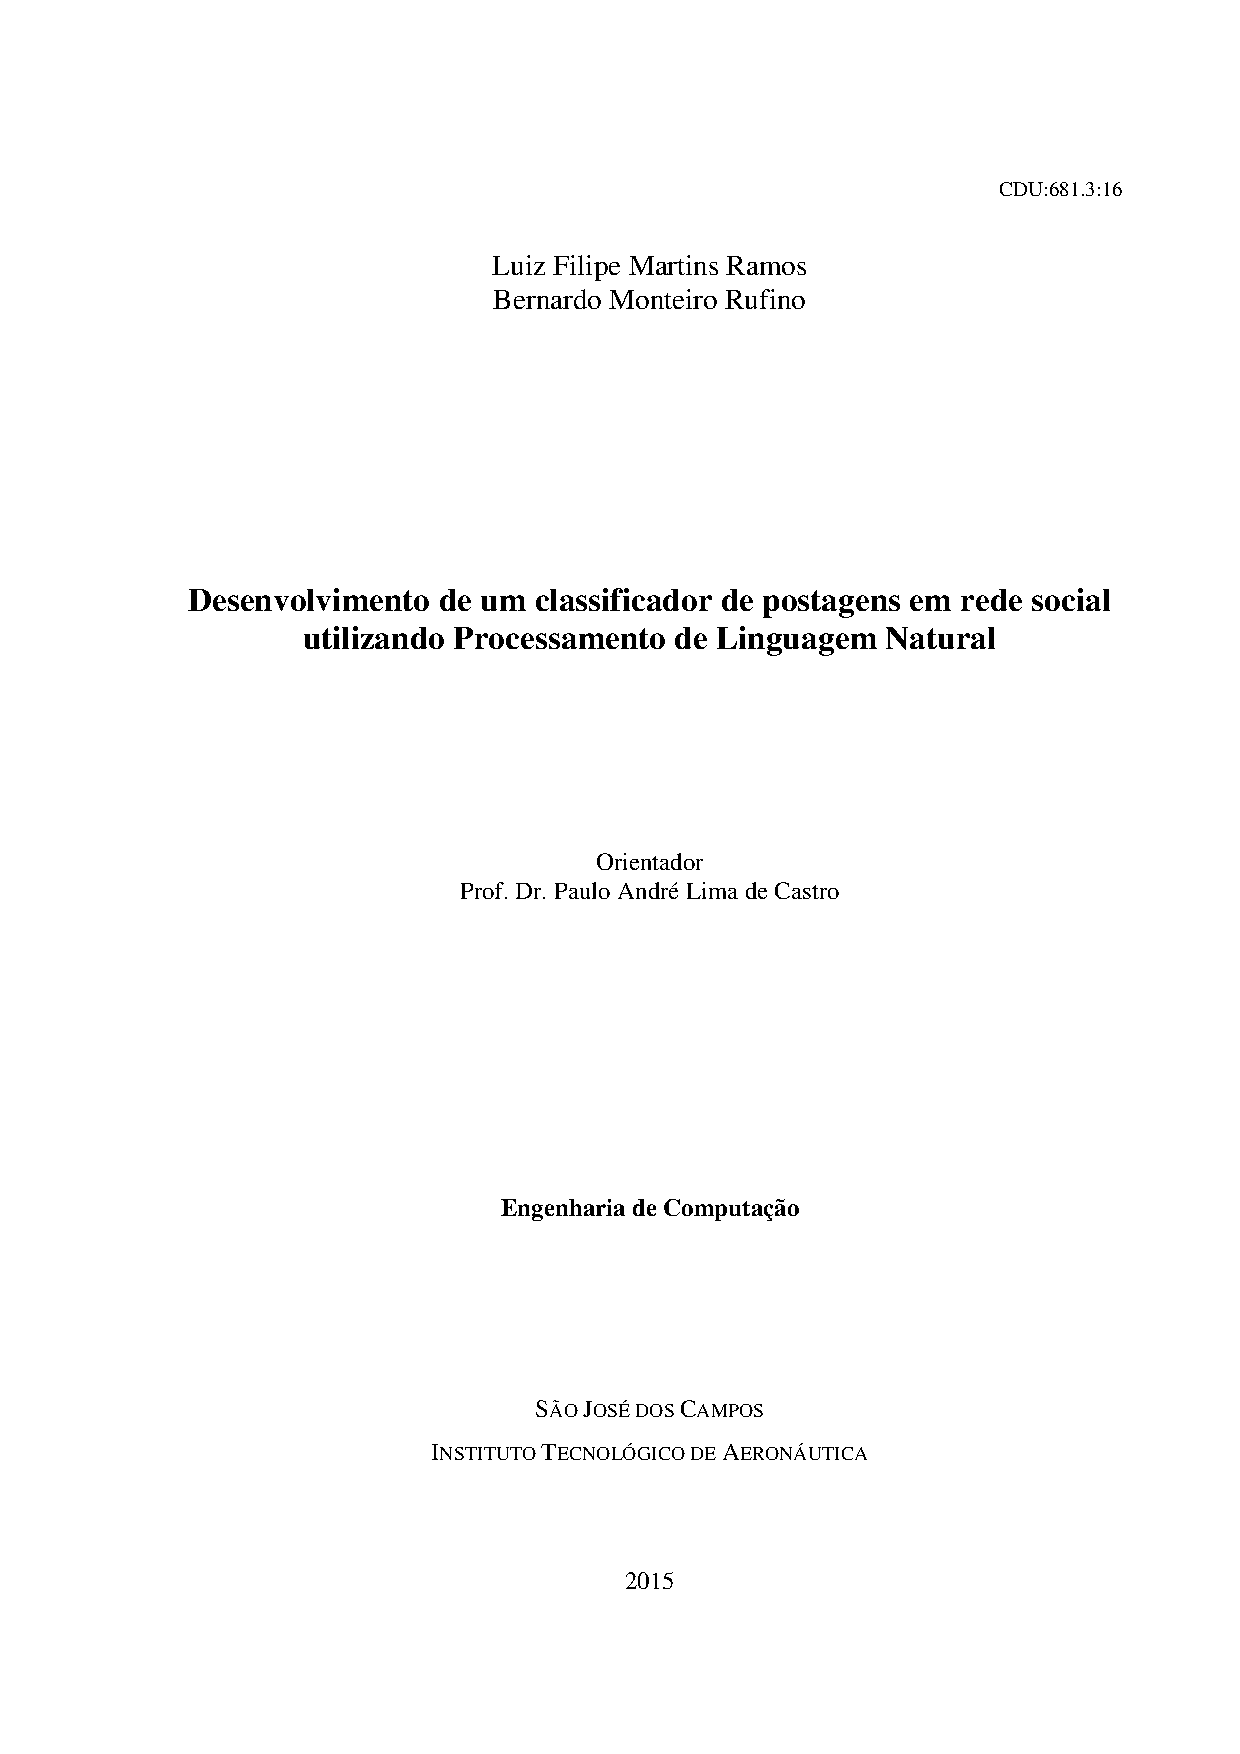
\includepdf{folha_rosto_tg.pdf}
\bookmark[level=0, page=2]{Folha de Rosto}

% TODO: Colocar numero da CDU na folha de rosto
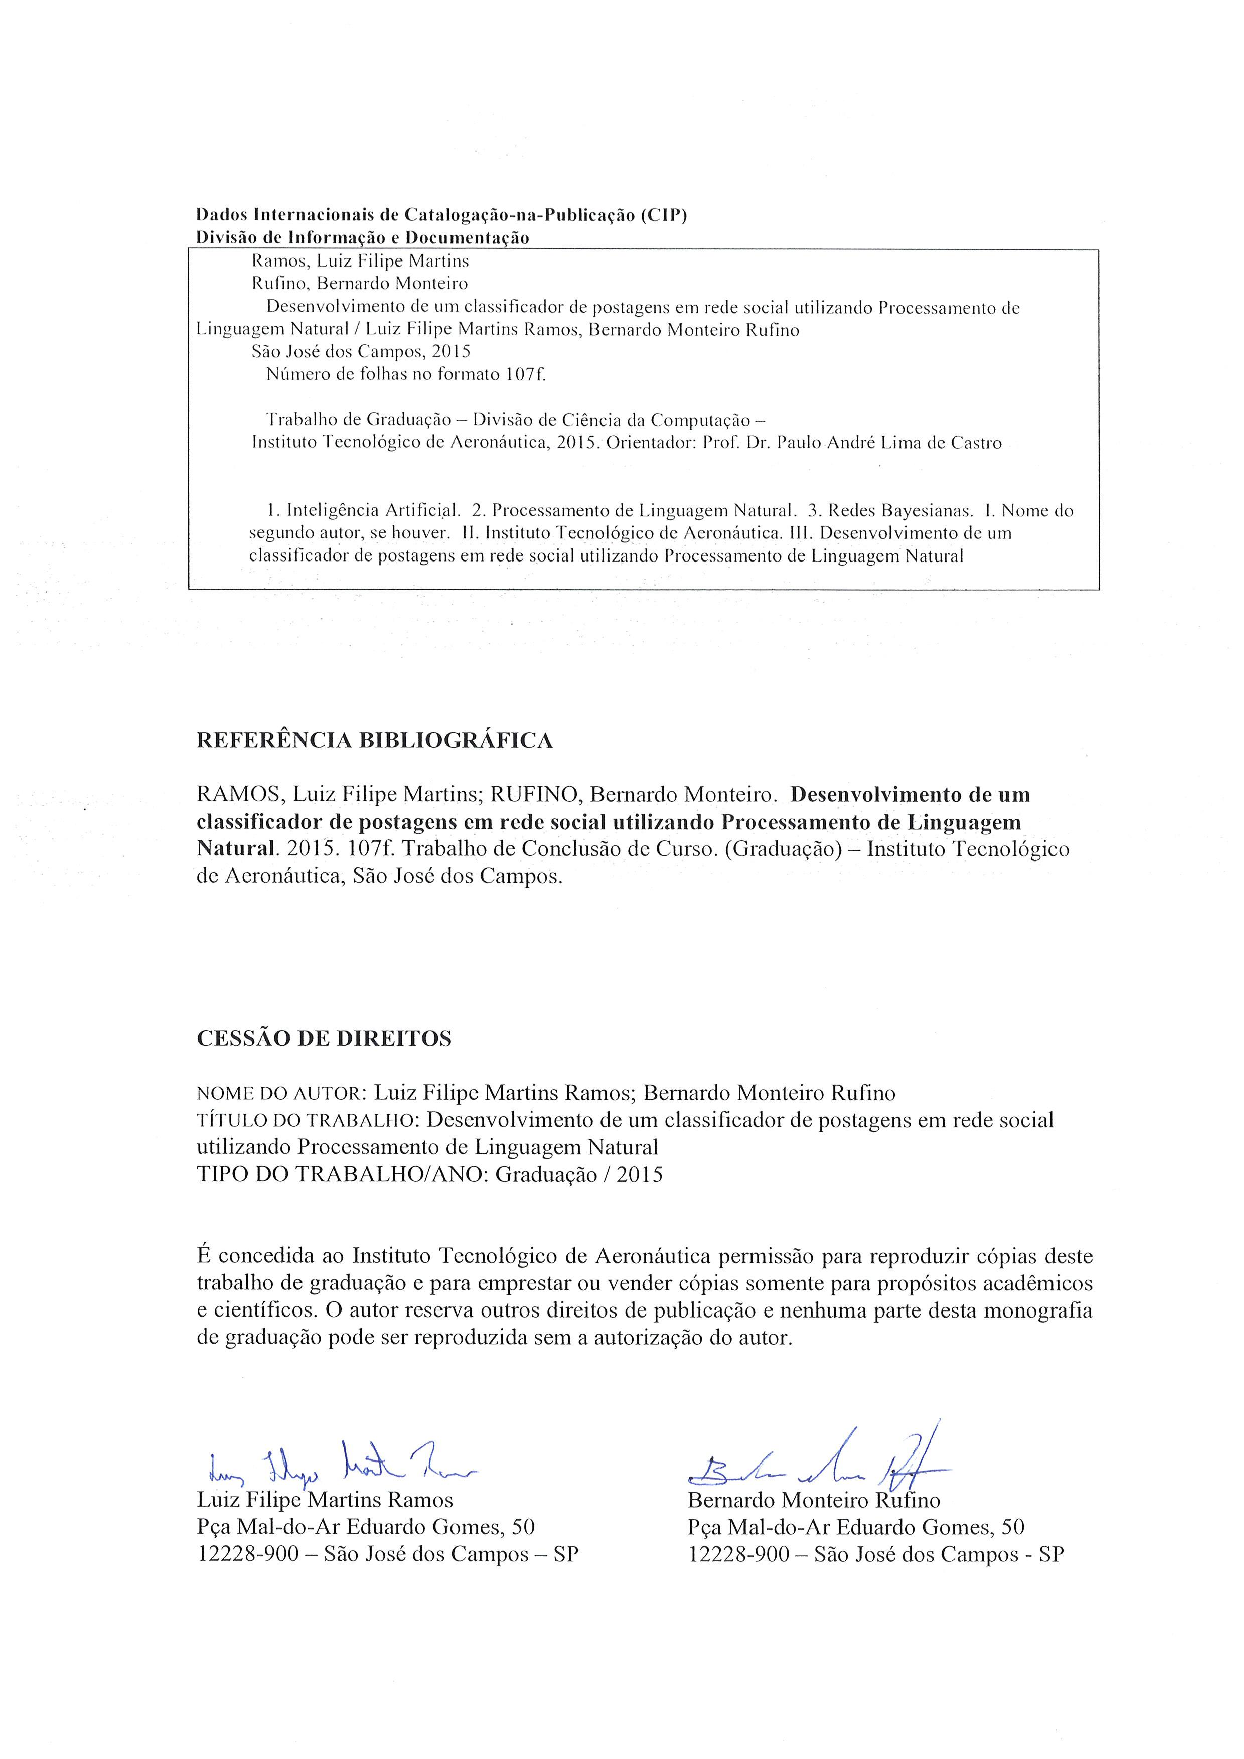
\includepdf{verso_folha_rosto_tg.pdf}
\bookmark[level=0, page=3]{Verso da Folha de Rosto}

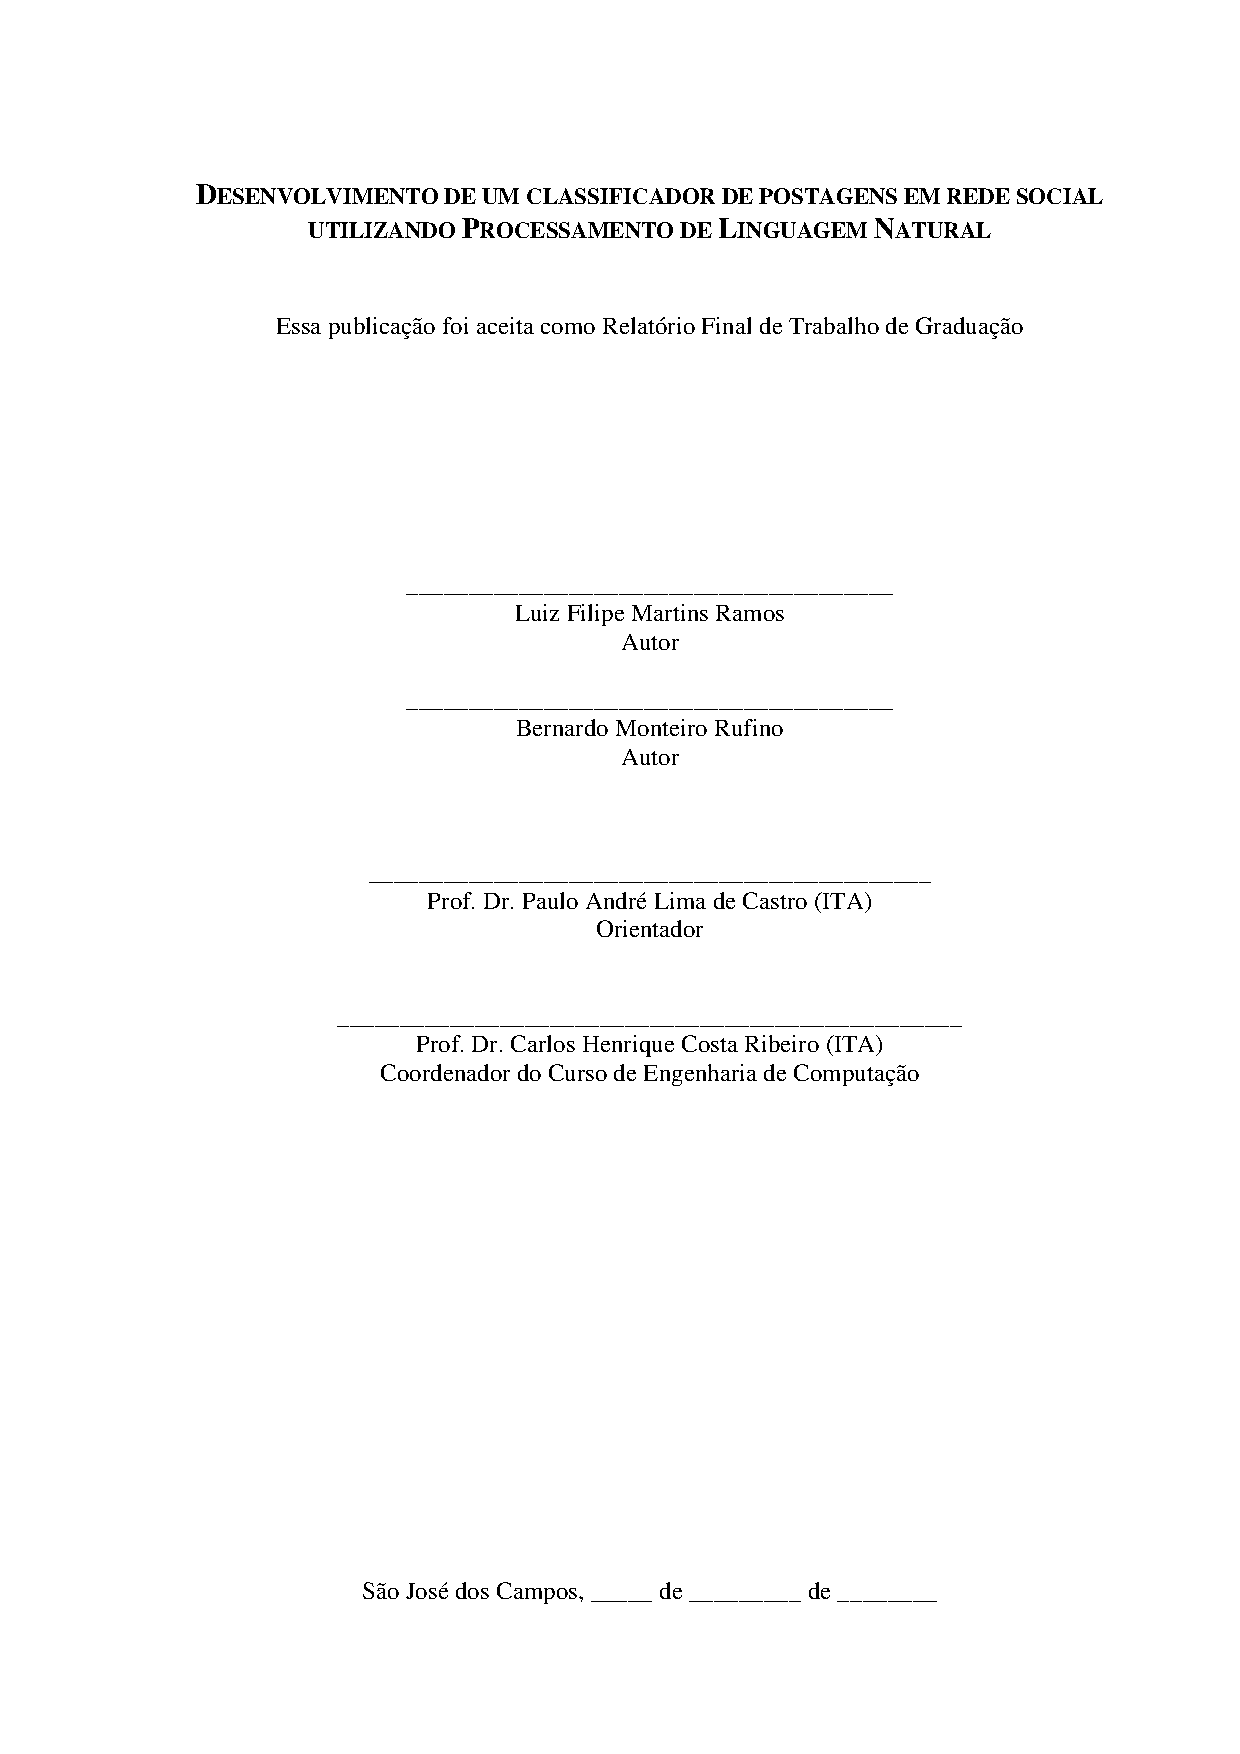
\includepdf{folha_aprovacao_tg.pdf}
\bookmark[level=0, page=4]{Folha de Aprova��o}

\vspace*{18cm}

\begin{flushright}
\begin{minipage}[t]{7.0 cm}
% TODO: Add dedicatoria
\end{minipage}
\end{flushright}
\thispagestyle{empty}
\bookmark[level=0, page=5]{Dedicat�ria}

\chapter*{Agradecimentos}
%TODO: Add agradecimentos

\newpage
\thispagestyle{empty}

\vspace*{15.0 cm}

% TODO: Change citacao
\textit{The question of whether a computer can think is no more interesting than the question of whether a submarine can swim.}

\begin{flushright}
Edsger W. Dijkstra
\end{flushright}

\iffalse
\vspace*{14.0 cm}

\noindent\textit{Dear Moore,}

\indent\textit{Your letter annoyed me. When I wrote Logik I didn't consult the Regulations, and therefore I think it would only be fair if you gave me my degree without consulting them so much either! As to a Preface and Notes; I think my examiners will easily see how much I have cribbed from Bosanquet. - If I'm not worth your making an exception for me even in some STUPID details then I may as well go to Hell directly; and if I am worth it and you don't do it then - by God - you might go there.}

\indent\textit{The whole business is too beastly to go on writing about it so -}

\noindent\textit{L.W.}

\begin{flushright}
(Carta de Ludwig Wittgenstein a George Moore)
\end{flushright}
\fi
\thispagestyle{empty}
\bookmark[level=0, page=7]{Cita��o}

\chapter*{Resumo}
Esta disserta��o prop�e-se a analisar o problema de classifica��o de textos no contexto de redes sociais (mais especificamente o Facebook). Inicialmente foram implementadas Multinomial Na�ve Bayes, utilizando como feature as palavras dos textos, e posteriormente foram inclu�dos metadados das postagens. Como os resultados n�o foram satisfat�rios, explorou-se um modelo de Weighted Na�ve Bayes com pesos baseados na Teoria da Informa��o, o que trouxe melhoras significativas na qualidade dos resultados.

A partir do classificador criado, desenvolveu-se uma extens�o para o navegador Chrome que modifica o feed de not�cias do Facebook adicionando um cabe�alho a cada postagem que contem o seu assunto. O usu�rio pode modificar o assunto, caso discorde da classifica��o automatizada, dando um feedback que permite uma aprendizagem online para as Redes Bayesianas constru�das.
\thispagestyle{empty}

\chapter*{Abstract}
This work analyses the problem of text classification in the context of social networks (Facebook, specifically). Multinomial Naïve Bayes were implemented using only words as features at first, and then some post's metadata too. As the results were not satisfying, a Weighted Naïve Bayes model was implemented with weights based on Information Theory, which really improved the classifier performance.

Afterwards, a chrome extension, that modifies the News Feed adding headers to each post with a corresponding tag, was developed. The user can modify this tag if he disagrees with the automatic classification and his feedback allows the Bayesian Network to learn online.
\thispagestyle{empty}

\tableofcontents
\bookmark[level=0, page=10]{Sum�rio}
\addtocontents{sumario}{\protect\thispagestyle{empty}}
%\thispagestyle{empty}
% TODO: Descobrir como tirar numera��o do Sum�rio

\listoffigures
%\thispagestyle{empty}
% TODO: Descobrir como tirar numera��o da lista de figuras

\listoftables
\thispagestyle{empty}

\listofalgorithms
\thispagestyle{empty}

\lstlistoflistings
\thispagestyle{empty}

% TODO: Completar lista de abreviaturas
\chapter*{Lista de Abreviaturas}
\begin{acronym}
\acro{NB}{Na�ve Bayes}
\end{acronym}
\thispagestyle{empty}

\chapter{Introdu��o}
\label{introducao}

% TODO: Write Initial Introduction

\section{Motiva��o}

% TODO: Write Motivacao

\section{Objetivos}

% TODO: Write Objetivos

\section{Organiza��o do Texto}

% TODO: Write Organizacao do Texto

\chapter{Defini��o do Problema}
Antes de se abordarem as solu��es propostas, � necess�rio entender com detalhes o problema que est� sendo analisado.

\section{O Problema de Classifica��o}
Em aprendizado de m�quina, o problema de classifica��o consiste na tarefa de atribuir a objetos uma ou mais das diversas categorias pr�-definidas \cite{introduction_to_datamining}. Ou seja, dado um objeto, o classificador deve ser capaz de identificar em qual categoria tal objeto se encaixa melhor, como pode ser visualizado na Figura \ref{fig:esquema_classificador}.

O problema de classifica��o em geral � o exemplo cl�ssico de aprendizado de m�quina supervisionado. A partir de um conjunto de exemplos previamente classificados por um supervisor experiente (em geral um ou mais humanos com conhecimento de dom�nio), o classificador � capaz de aprender e generalizar, podendo assim categorizar corretamente novos objetos encontrados.

Existem v�rios tipos diferentes de classifica��o baseados na quantidade de categorias pr�-definidas bem como na quantidade de classes �s quais cada objeto pode pertencer.

\begin{figure}[ht!]
	\centering
	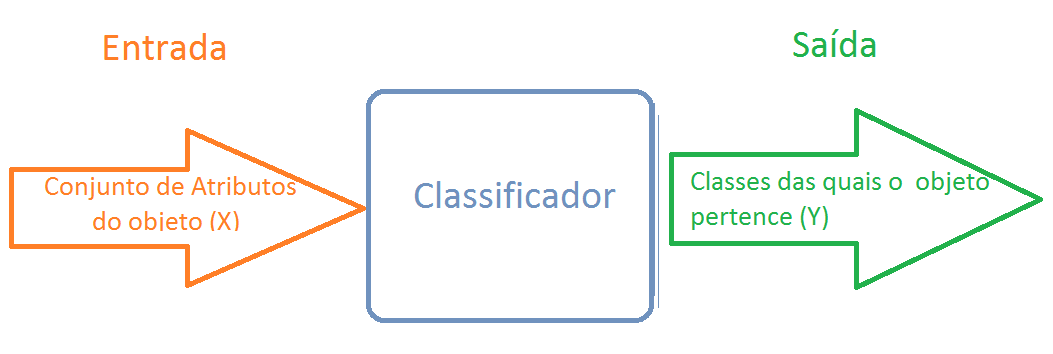
\includegraphics[width=0.9\textwidth]{esquema_classificador.png}
	\caption{Esquema ilustrativo da fun��o de um classificador}
	\label{fig:esquema_classificador}
\end{figure}

\subsection{Classifica��o Bin�ria}

A classifica��o bin�ria � o caso mais simples que pode ser estudado. Neste problema, h� apenas duas classes diferentes e cada objeto pertence a exatamente uma delas. 

Exemplos comuns que podem ser citados s�o a classifica��o de emails em spam ou n�o-spam, a classifica��o de tumores em benignos ou malignos, a determina��o de quais produtos dever�o ser descartados em uma linha de produ��o, a detec��o de transa��es financeiras fraudulentas, etc.

\subsection{Classifica��o \emph{Multi-Class}}
Quando h� mais de duas classes poss�veis, chama-se o problema de classifica��o \emph{multi-class}. Neste caso, cada objeto deve pertencer a exatamente uma dentre as v�rias categorias pr�-definidas. O classificador deve ser capaz de determinar qual � a categoria de cada objeto.

V�rios exemplos de classifica��o podem ser considerados. Dadas imagens de frutas (que podem ser ma��s, peras, ou laranjas) determinar qual � o tipo de cada fruta. Ou ent�o dadas imagens de telesc�pio de galaxias distantes, determinar o tipo da galaxia em quest�o (el�ptica, espiral, etc).

\subsection{Classifica��o \emph{Multi-Class / Multi-Label}}
Quando h� v�rias classes poss�veis (mais de duas) e cada objeto pode pertencer a mais de uma classe, chama-se o problema de \emph{multi-class / multi-label}. Este � o mais dif�cil dos tr�s problemas apresentados, uma vez que h� diversas poss�veis combina��es de classes para cada objeto.

A classifica��o de textos � um cl�ssico exemplo de classifica��o \emph{multi-class / multi-label}, j� que o texto pode pertencer a uma ou varias classes simultaneamente.

Para resolver o problema de classifica��o \emph{multi-class / multi-label} podem ser utilizadas duas abordagens diferentes. Uma delas � a abordagem \emph{one vs all} e a outra � a abordagem dos subconjuntos.

Na abordagem \emph{one vs all}, para cada classe, realiza-se a classifica��o bin�ria do objeto em \emph{pertence} ou \emph{n�o pertence} a esta classe. Desta forma, determina-se todas as classes �s quais o dado objeto pertence. O problema desta abordagem � que pequenos erros que fa�am com que o classificador de uma das classes n�o fique bom (dados ruins para uma classe por exemplo) torna o resultado inteiro ruim.

Na abordagem de subconjuntos, consideram-se todos os poss�veis subconjuntos das classes (com 1, 2, 3, ..., L elementos, onde L � o total de classes) e escolhe-se o subconjunto desejado (utilizando um classificador multi-class). O grande problema desta abordagem � que ha $2^{L - 1}$ poss�veis subconjuntos da classes (o que pode ser muito).

\section{Objeto de Estudo deste Trabalho}
Como foi visto, a classifica��o de textos � um problema do tipo \emph{multi-class / multi-label}, entretanto seria necess�ria uma quantidade muito grande de dados para se obter resultados satisfat�rios neste problema. Portanto, fez-se a simplifica��o de considerar o problema apenas \emph{multi-class}, ou seja, cada texto s� ser� classificado em um �nica classe.
% TODO: Talvez tentar multi class multi label com 1/2/3 classes?



\chapter{Fundamenta��o Te�rica}
\section{Defini��o formal}
Utilizando a nota��o adotada por Dan Jurafsky e Christopher Manning em seu curso de Processamento de Linguagem Natural para Stanford \cite{text_classification}, define-se o problema da classifica��o supervisionada de textos da seguinte forma.

Seja $C=\{c_1, c_2, ..., c_J\}$ um conjunto fixo de classes, $D=\{d_1, d_2, ..., d_n\}$ um conjunto de documentos, e $\mathcal{T}=\{(d_1, c_{d_1}), (d_2, c_{d_2}), ... , (d_m, c_{d_m})\}$ um conjunto de treinamento (subconjunto de $D$) com $m$ documentos classificados manualmente, o classificador consiste em uma fun��o $\gamma :D\rightarrow C$ que relaciona um documento a uma classe, e um algoritmo de aprendizado de m�quina supervisionado � um algoritmo que recebe como par�metros $C$ e $\mathcal{T}$ e retorna $\gamma$.

\section{Tipos de classificadores}
Existem diversos tipos diferentes de classificadores que possuem resultados muito bons dependendo do problema analisado. Segue abaixo uma lista dos principais classificadores existentes.

\begin{itemize}	
	\item �rvores de Decis�o
	\item Na�ve Bayes
	\item Regress�o Log�stica
	\item Support Vector Machines
	\item k-Nearest Neightbors
	\item Redes Neurais
	\item Dentre outros
\end{itemize}

A performance de todos estes m�todos varia consideravelmente dependendo da aplica��o. Estudos mostram que para bases de dados grandes o suficiente, �timos resultados podem ser atingidos independentemente do m�todo utilizado \cite{practical_issues}. Entretanto, para uma quantidade pequena de dados as Na�ve Bayes apresentam resultados bons por serem classificadores de alto \emph{bias} / baixa vari�ncia \cite{quora_classifier}. 

As NB possuem as vantagens de serem f�ceis de se implementar, serem bem r�pidas na hora da execu��o e mostrarem bons resultados pr�ticos.

\section{Redes Bayesianas}

\subsection{Defini��o}
Em modelagem gr�fica probabil�stica, Redes Bayesianas s�o grafos direcionados que representam rela��es de depend�ncia condicionais entre diferentes vari�veis aleat�rias \cite{introduction_to_graphical_models}. A partir da visualiza��o de uma Rede Bayesiana � poss�vel utilizar a regra de Bayes para realizar infer�ncias e descobrir a probabilidade de eventos, dadas algumas vari�veis observadas.As arestas direcionadas representam as no��es de causalidade entre as vari�veis aleat�rias e geram as depend�ncias condicionais. Para cada n� do gr�fico deve haver uma tabela de probabilidades condicionais para a vari�vel em quest�o.

A Figura \ref{fig:bayesian_networks}, retirada do curso de Modelagem Gr�fica Probabil�stica da professora Daphne Koller de Stanford \cite{probabilistic_graphical_models}, ilustra um exemplo de uma Rede Bayesiana simples. Neste caso, pode-se ver que a nota do aluno � influenciada pela dificuldade da prova e pela sua inteligencia. Alem disso A possibilidade do professor escrever uma carta de recomenda��o depende apenas da nota do aluno e o SAT do aluno depende apenas de sua inteligencia. Em cada n� do grafo h� uma tabela de distribui��es de probabilidades condicionais.

\begin{figure}[ht!]
	\centering
	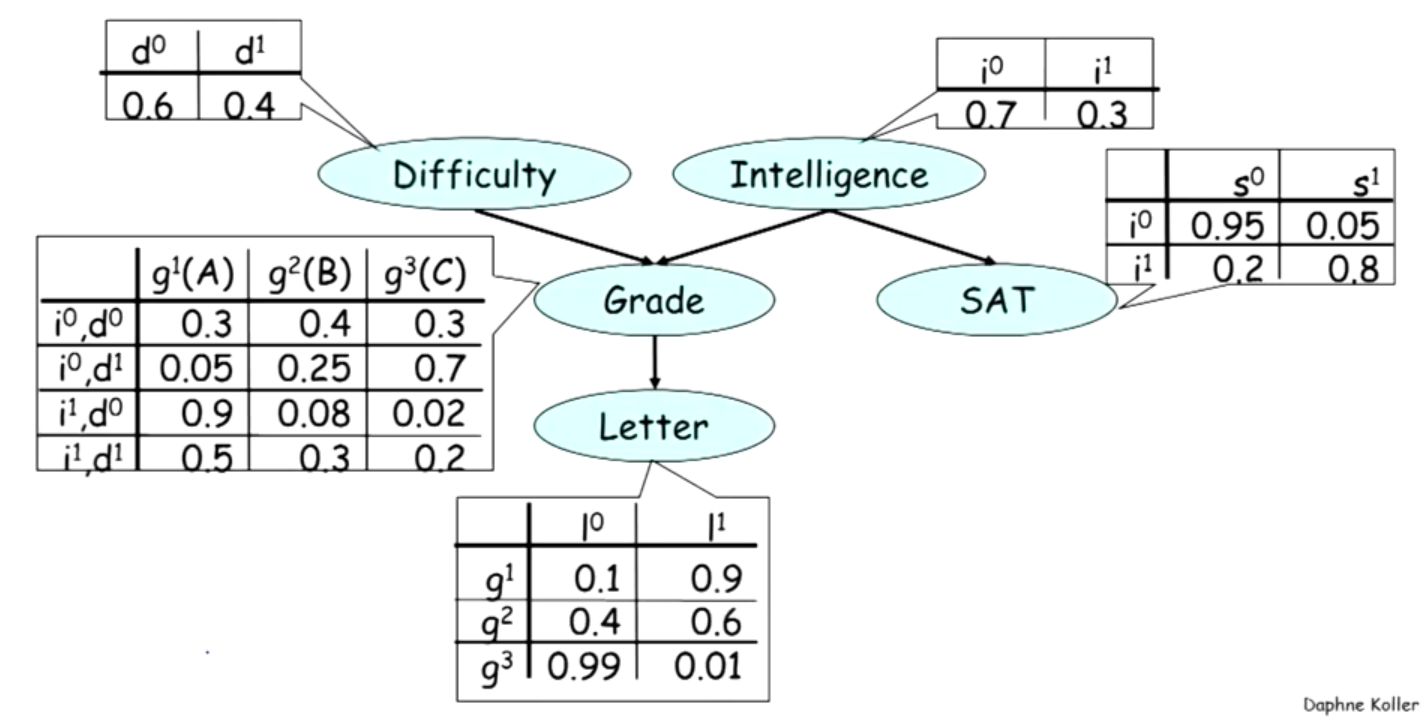
\includegraphics[width=0.9\textwidth]{bayesian_networks.png}
	\caption{Exemplo de Redes Bayesianas}
	\label{fig:bayesian_networks}
\end{figure}


\subsection{Regra de Bayes}
Para realizar infer�ncias nas redes Bayesianas utiliza-se a regra de Bayes, como definida a seguir.

Sejam $A$ e $B$ dois eventos com probabilidades de ocorr�ncia $P(A)$ e $P(B)$ e sendo $P(A|B)$ e $P(B|A)$ as probabilidades condicionais de $A$ dado $B$ e de $B$ dado $A$, respectivamente, tem-se que:

$P(A|B) = \frac{{P(A) P(B|A)}}{P(B)}$

Esse resultado parte da no��o probabilidade conjunta $P(A,B)$.

$P(A,B)=P(A) P(B|A) = P(B) P(A|B) \rightarrow P(A|B) = \frac{{P(A) P(B|A)}}{P(B)}$

No caso do exemplo da Figura \ref{fig:bayesian_networks}, podemos calcular a probabilidade conjunta da rede da seguinte forma:

$P(D,I,G,S,L)=P(D)P(I)P(G|I,D)P(S|I)P(L|G)$ 

Onde $D=Difficulty$, $G=Grade$, $I=Intelligence$, $S=SAT$ e $L=Letter$.

\subsection{Na�ve Bayes}
\subsubsection{Problema a ser resolvido}
Redes Bayesianas s�o ferramentas excelentes para modelar problemas complexos, entretanto elas possuem um grande problema pr�tico. A realiza��o de infer�ncias em redes gen�ricas � um problema NP-hard, conforme demonstrado por Cooper \cite{inference_bayesian_networks}.

O que � realizado na pr�tica �, ou realizar infer�ncias aproximadas nas redes com algoritmos polinomiais, ou simplificar as redes a alguns tipos espec�ficos mais simples.

\subsubsection{O que s�o Na�ve Bayes}
As Na�ve Bayes (bayes ing�nuas) s�o simplifica��es feitas na modelagem de um problema por redes Bayesianas de modo a tornar poss�vel realizar a infer�ncia de forma r�pida. Elas assumem que as vari�veis do problema s�o condicionalmente independentes (mesmo que na pr�tica elas n�o sejam, o que explica o nome \emph{ing�nuas}).

A Figura \ref{fig:naive_bayes_example} mostra um exemplo de uma NB comum. Ela possui uma vari�vel $Classe$ que depende de um s�rie de outras var�veis $x_1, x_2, x_3, ... , x_n$ (que ser�o chamadas a partir daqui de features). � importante notar que a estrutura da rede mostra que as features s�o condicionalmente independentes umas das outras e a $Classe$ depende de cada uma das features individualmente. � f�cil entender a grande vantagem desta abordagem. Cada tabela de probabilidades condicionais ser� pequena. Alem disso a infer�ncia da vari�vel classe, dadas algumas das features ser� bem simples, como ser� mostrado nas pr�ximas se��es.

\begin{figure}[ht!]
	\centering
	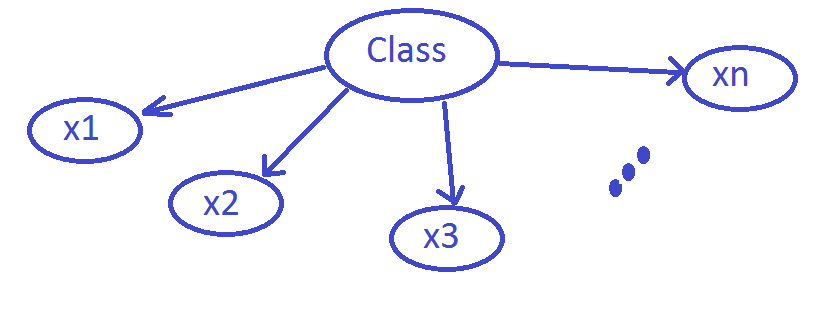
\includegraphics[width=0.9\textwidth]{naive_bayes_example.png}
	\caption{Exemplo de uma Na�ve Bayes}
	\label{fig:naive_bayes_example}
\end{figure}

Na pr�tica o NB � um �timo classificador de textos, pois, al�m de ser simples, traz resultados compar�veis a outros classificadores substancialmente mais complexos e lentos.

\subsubsection{Independ�ncia Condicional}
Antes de explicar a infer�ncia em NB � importante entender o que significa o conceito de independ�ncia condicional.

Dados dois eventos $A$ e $B$, dizemos que eles s�o independentes se a probabilidade de ocorr�ncia de um deles n�o � influenciada pelo fato do outro ter ocorrido. Ou seja:

$P(A|B) = P(A)$
$P(B|A) = P(B)$

Esta propriedade � muito relevante na simplifica��o de express�es pois podemos usar o fato de que a probabilidade conjunta � igual ao produto das probabilidades individuais.

$P(A,B) = P(A)P(B|A) = P(A)P(B)$

\subsubsection{Infer�ncia}
A regra de Bayes seguida pela propriedade de independ�ncia condicional pode ser utilizada para a realiza��o de infer�ncia em NB da seguinte forma.

Sejam $C=\{c_1,c_2,c_3, ..., c_J\}$ um conjunto de classes e $x_1, x_2, x_3, ..., x_n$ as features a serem analisadas. Como trata-se de NB, assume-se independ�ncia condicional das features. Deseja-se saber para cada $i$:

$P(C=c_i|x_1,x_2,...,x_n)$

Ou seja, deseja-se saber qual a probabilidade da classe possuir o valor $c_i$, dadas as features observadas.

Pela regra de Bayes temos:

\begin{equation}
P(C=c_i|x_1,x_2,...,x_n) = \frac{P(x_1,x_2,...,x_n|C=c_i)P(C=c_i)}{P(x_1,x_2,...,x_n)}
\label{eq:bayes_inference}
\end{equation}

Como $x_1, x_2, x_3, ..., x_n$ s�o condicionalmente independentes entre si, temos:


\begin{equation}
\begin{split}
P(x_1,x_2,...,x_n|C=c_i) &= P(x_1,x_2,...,x_{n-1}|x_n,C=c_i)P(x_n|C=c_i) \\ 
&= P(x_1,x_2,...,x_{n-1}|C=c_i)P(x_n|C=c_i) \\
&= P(x_1,x_2,...,x_{n-2}|x_{n-1},C=c_i)P(x_{n-1}|C=c_i)P(x_n|C=c_i) \\
&= P(x_1,x_2,...,x_{n-2}|C=c_i)P(x_{n-1}|C=c_i)P(x_n|C=c_i) \\
&= ... = P(x_1|C=c_i)P(x_2|C=c_i)P(x_3|C=c_i)...P(x_n|C=c_i)  \\
&= \prod_{j=1}^{n}P(x_j|C=c_i)
\end{split}
\label{eq:produtorio}
\end{equation}


Substituindo \ref{eq:produtorio} em \ref{eq:bayes_inference} temos:

\begin{equation}
P(C=c_i|x_1,x_2,...,x_n) = \frac{P(C=c_i)({\prod_{j=1}^{n}P(x_j|C=c_i)})}{P(x_1,x_2,...,x_n)}
\label{eq:naive_bayes_probability}
\end{equation}

\subsubsection{Classifica��o utilizando Na�ve Bayes}
No problema de classifica��o temos um documento $d$ que ser� representado pelas features $x_1,x_2,...,x_n$ e deseja-se saber de qual classe $c \in C$ este documento pertence.

Matematicamente, deseja-se saber de qual classe � mais prov�vel que o documento perten�a. Isto �, a classe que maximiza $P(d|c)$.

$\gamma(d)=argmax_c(P(d|c))=argmax_c(P(x_1,x_2,...,x_n|c))$

Pela equa��o \ref{eq:naive_bayes_probability}, temos que:

$argmax_c(P(x_1,x_2,...,x_n|c)) = argmax_c(\frac{P(C=c_i)({\prod_{j=1}^{n}P(x_j|C=c_i)})}{P(x_1,x_2,...,x_n)})$

Como $P(x_1,x_2,...,x_n)$ n�o depende de c, pode-se cort�-lo do denominador, chegando em:

$\gamma(d) = argmax_c(P(C=c_i)({\prod_{j=1}^{n}P(x_j|C=c_i)})$

Agora, para descobrir a classe do documento, basta calcular $P(C=c_i)$ e $P(x_k|C=c_i)$ e ambas estas probabilidades s�o f�ceis de serem estimadas (se tivermos um conjunto de treino suficientemente grande).

Assumindo que as features sejam binarias, isto �, ou est�o presentes no documento, ou n�o est�o. Seja $\#(x)$ um operador que indica quantas vezes a feature x aparece no conjunto de treinamento e $\#(c)$ quantos documentos do conjunto de treinamento possuem a classe c. Al�m disso, seja $\#(x \wedge c)$ a quantidade de vezes que a feature x aparece num documento de classe c e seja N o total de documentos do conjunto de treinamento. � f�cil ver que:

$P(C=c_i) \simeq \frac{\#(c_i)}{N}$

e

$P(x_j|C=c_i) \simeq \frac{\#(x_j \wedge c_i)}{\#(c_i)}$

Ou seja, o problema de classifica��o se tornou basicamente um problema de contagem.

\subsubsection{Smoothing}
Um dos problemas pr�ticos encontrados por NB � a ocorr�ncia de contagens nulas. O grande problema do 0 � que se ele for apenas um dos fatores da multiplica��o o resultado inteiro ser� 0, inutilizando o m�todo.

Isto n�o � algo incomum, principalmente se o conjunto de treinamento for pequeno. Basta ter uma palavra no conjunto de teste que nunca ocorreu em uma determinada classe no conjunto de treinamento.

Existem t�cnicas que s�o utilizadas para resolver este problema e elas s�o chamadas de Smoothing. Neste trabalho utilizou-se uma das mais comuns: o Laplace Smoothing.

O Laplace consiste em assumir que todas as features foram vistas pelo menos $\alpha$ vezes em cada uma das classes. Isso se traduz nas seguintes formulas, sendo $L$ o n�mero total de classes e $V$ o numero total de features.

$P(C=c_i) \simeq \frac{\#(c_i) + \alpha}{N + \alpha L}$

e

$P(x_j|C=c_i) \simeq \frac{\#(x_j \wedge c_i) + \alpha}{\#(c_i) + \alpha V}$

No caso especial em que $\alpha = 1$, tem-se o \emph{Add-One Smoothing}.

\subsection{Modelagens para classifica��o de texto}
Uma vez que j� foi entendida a forma de classificar o texto, resta apenas represent�-lo por um conjunto de features.

\subsubsection{Na�ve Bayes Bin�ria}
Uma forma comum de representar um texto em features � consider�-lo como um conjunto de palavras. Assume-se que cada palavra � uma feature que pode estar presente ou n�o no documento. Nesta representa��o a ordem das palavras n�o � importante.

Esta representa��o n�o leva em considera��o a frequ�ncia com a qual cada palavra aparece no texto. A f�rmula para calcular a classe mais prov�vel � aquela que foi desenvolvida acima.

% TODO: Continuar essa explica��o

\subsubsection{Na�ve Bayes de Bernoulli}

\subsubsection{Multinomial Na�ve Bayes}
� interessante levar em considera��o a frequ�ncia da ocorr�ncia das palavras uma vez que esta pode trazer informa��o relevante sobre a classe.
% TODO: Entender multinomial bayes e continuar


\subsubsection{Outras features}
� poss�vel enriquecer o classificador utilizando outras features (que n�o sejam as pr�prias palavras do texto). Exemplos de features que podem ser utilizadas s�o: combina��es de palavras, o tamanho do texto, quantidade de sinais de pontua��o, quantidade de palavras com iniciais mai�sculas, etc.

Para o caso espec�fico de postagens em redes sociais existem ainda outras features que podem ser inclu�das. Pode-se considerar o autor da postagem, o momento em que ela foi publicada, a presen�a de fotos, v�deos ou links, etc.

\section{Weighted Na�ve Bayes}
Um dos problemas das NB � que muitas vezes nas aplica��es reais n�o � poss�vel assumir a independ�ncia condicional das features. Muitas vezes uma das features tem um peso maior que as outras, por exemplo.

Um modo inicial de relaxar essa hip�tese de independ�ncia, � eliminar features com alta correla��o, fazendo com que o subconjunto restante se encaixe melhor na hip�tese de independ�ncia condicional. Isto � chamado de sele��o de features.

Neste caso temos:

$\gamma(d) = argmax_c(P(C=c_i)({\prod_{j=1}^{n}P(x_j|C=c_i)^{I(j)}})$

Onde:

$I(j) \in \{0,1\}$

Uma abordagem mais gen�rica � ponderar cada feature de acordo com sua relev�ncia. Ou seja:

$\gamma(d) = argmax_c(P(C=c_i)({\prod_{j=1}^{n}P(x_j|C=c_i)^{w(j)}})$

Onde:

$w(j) \in \mathbb{R}^+$

Nota-se que a sele��o de features � um caso espec�fico da pondera��o de features (onde $w(j)$ s� pode ser 0 ou 1).

Agora o grande problema passa a ser determinar os pesos $w(j)$ das features. H� diversos algoritmos que ja foram propostos para realizar esta tarefa.

% TODO: Escrever sobre outros approachs the feature weighting (tem naquele artigo)

Neste trabalho, estudou-se a utiliza��o de um m�todo baseado na Teoria da Informa��o, que al�m de ser comum na literatura, possui fundamentos te�ricos bem embasados \cite{weighted_naive_bayes}. 

% TODO: Escrever sobre feature weighting


\section{M�todos de avalia��o de um classificador}
Uma vez desenvolvido o classificador � importante ser capaz de avali�-lo a fim de determinar o qu�o bom ele �. A utiliza��o de m�tricas num�ricas para avaliar os classificadores � interessante pois permite a realiza��o de compara��es entre as diferentes vers�es implementadas, tornando poss�vel determinar se as modifica��es que foram feitas est�o fazendo efeito.

Existem diversas m�tricas que podem ser utilizadas para avaliar classificadores, algumas delas ser�o analisadas nesta se��o.

\subsection{Classificador Bin�rio}

\subsubsection{Acur�cia}

\subsubsection{Precis�o}

\subsubsection{Abrang�ncia (\emph{Recall})}

\subsubsection{Medida F1}

\subsection{Classificador \emph{Multi-Class}}

\subsubsection{Matriz de Confus�o (\emph{Confusion Matrix})}

\subsubsection{M�dias micro e macro (\emph{Micro and Macro Averaging})}

\subsubsection{Medida Kappa}





\chapter{Metodologia}
\section{Plano de desenvolvimento}

Dividiu-se o desenvolvimento do projeto em diversas etapas.

\subsection{Estudo basico sobre Processamento de Linguagem Natural}
Inicialmente realizou-se um estudo aprofundado sobre o assunto do projeto para aproveitar o conhecimento j� desenvolvido ao longo dos anos pela comunidade cient�fica e garantir que as melhores tecnologias e t�cnicas fossem adotadas.
O plano de estudos adotado foi:

\begin{enumerate}[(a)]
\item Express�es regulares
\item Processamento de texto
\item Normaliza��o
\item Tokeniza��o das strings
\item Modelagem lingu�stica e simplifica��o de N-gramas
\item Classifica��o de texto
\item Na�ve Bayes
\item M�tricas de performance (Precis�o, Abrang�ncia, Acur�cia, etc)
\item Melhorias para Na�ve Bayes
\end{enumerate}

\subsection{Coleta de dados}
Como trata-se de um projeto de Intelig�ncia Artificial, � essencial que se obtenha uma base de dados grande o suficiente para que o sistema desenvolvido seja capaz de realizar as generaliza��es necess�rias para um bom funcionamento sem que haja overfit.

Esta base de dados consiste em um conjunto de postagens (vari�vel X) e o assunto da mesma (vari�vel Y).

Foram propostas duas formas poss�veis de aquisi��o de dados.

\begin{itemize}
\item Uma delas foi desenvolver um plugin que colete as postagens e pergunte o assunto para o usu�rio. A utiliza��o deste plugin por v�rias pessoas permitiu a aquisi��o de uma base de dados consider�vel.
\item Paralelamente desenvolveram-se crawlers para vasculhar sites que contenham artigos e textos sobre cada assunto que se deseja classificar. � importante ter a capacidade de classificar artigos de sites gen�ricos, pois muitas das postagens em rede social possuem links para tais sites.
\end{itemize}

\subsection{Pr�-processamento dos textos e normaliza��o}
Como trata-se de linguagem natural e ainda por cima coloquial, para atingir um bom resultado com o classificador � essencial que haja um bom pr�-processamento do texto corrigindo palavras erradas, frases mal-constru�das, normalizando termos parecidos, etc.


\subsection{Cria��o dos classificadores de Redes Bayesianas}
Foram criados classificadores de NB e suas performances foram avaliadas contra um conjunto de valida��o. Os m�todos mais efetivos foram selecionados, combinando os classificadores de postagens e de artigos e ajustando seus par�metros para obter um bom resultado final.

\subsection{Estudo dos resultados obtidos no conjunto de valida��o para diferentes features e par�metros}
\label{sec:validacao}
Foi realizado um estudo detalhado dos resultados obtidos pelos classificadores para diferentes features, par�metros e t�cnicas de classifica��o (NB e NB com pesos). A avalia��o final da rede foi realizada em um conjunto de teste separado. 

Separou-se a base de dados total em dois conjuntos. Um de treinamento e um de valida��o de forma aleat�ria, sendo 25\% para valida��o e 75\% para treinamento. Para a an�lise da qualidade do classificador realizou-se a m�dia das estat�sticas avaliadas para varias divis�es aleat�rias diferentes de modo a obter um resultado est�vel.

\subsection{Defini��o da arquitetura do classificador e sua implementa��o}
Definiu-se que a rede seria treinada e armazenada em um servidor central. Considerou-se tamb�m a possibilidade da rede ser din�mica (ou seja, se a intera��o com o usu�rio fazer com
que a rede aprenda online com as novas informa��es).

\subsection{Desenvolvimento do plugin}
Por fim desenvolveu-se o plugin para o Google Chrome, com uma interface gr�fica amig�vel para o usu�rio para que ele entenda de forma f�cil como filtrar as postagens em seu feed de not�cias. %TODO: Nao fizemos isto ainda

\subsection{Testes de usabilidade}
% TODO: Tirar isso daqui?
Por fim foram realizados testes de usabilidade com colegas de turma baseados nas heur�sticas de Nielsen.


\section{Aquisi��o de dados}
Como j� foi dito, foram desenvolvidas duas formas diferente de realizar a aquisi��o de dados. Uma delas consiste numa extens�o para o Google Chrome que possibilita o usu�rio classificar cada postagens � qual ele se depara no Facebook, enviando os dados e a classifica��o da mesma para o banco de dados. A outra forma de aquisi��o de dados � o desenvolvimento de um crawler que faz o download diversos artigos online.

\subsection{Extens�o do Chrome de classifica��o de postagens}
\label{sec:plugin_chrome}
\subsubsection{Funcionamento de extens�es do Chrome}
Extens�es s�o softwares que melhoram as funcionalidades de um navegador. O Google Chrome disponibiliza um Framework de desenvolvimento de extens�es com muitas capacidades \cite{chrome_extension}.

A extens�o consiste em um conjuntos de arquivos zipados que incluem HTML, Javascript, CSS, imagens, etc. O Javascript de uma extens�o pode ser dividido em 3 partes diferentes: c�digo de extens�o (\emph{extension code}), scripts de conte�do (\emph{content scripts}) e scripts injetados (\emph{injected scripts}). Estes tr�s modos foram descritos abaixo.

\begin{itemize}
\item \textbf{C�digo de extens�o:} Trata-se do c�digo injetado diretamente no browser, tendo portanto acesso a todas as funcionalidades da API do Chrome, como tabs de background, pop-ups do navegador (aqueles pequenos �cones das extens�es que ficam no canto superior direito do chrome), etc.

\item \textbf{Scripts de conte�do:} Trata-se de um c�digo que � executado quando uma determinada p�gina � carregada pelo usu�rio. Este script possui um escopo entre o do c�digo de extens�o e o do script injetado. Os scripts de conte�do t�m acesso � algumas das funcionalidades da API do Chrome e ao mesmo tempo pode acessar e modificar o DOM da p�gina. Por estar em um escopo diferente ao escopo do javascript da pr�pria p�gina ele n�o tem acesso �s fun��es e objetos definidos no mesmo. Por outro lado, ele n�o possui diversas das restri��es de seguran�a que scripts injetados possuem. O script de conte�do pode, por exemplo, executar cross-origin requests (ou seja, acessar servidores de outra origem).

\item \textbf{Scripts injetados:} Scripts injetados s�o, como o nome diz, peda�os de c�digo javascript que s�o injetados numa determinada p�gina, executando em seu escopo. Desta forma eles tem acesso � todas as fun��es e vari�veis definidos pelo javascript original da p�gina. Tamb�m podem modificar como eles quiserem estas vari�veis e o pr�prio DOM.

\end{itemize}

No caso da aplica��o deste trabalho, � necess�rio ser capaz de mandar os dados das postagens com suas classifica��es para um servidor central (que obviamente n�o � do pr�prio Facebook), logo scripts injetados n�o s�o uma boa solu��o (uma vez que o javascript do Facebook impede a execu��o de cross-origin requests). Ou seja, a extens�o foi desenvolvida predominantemente com scripts de conte�do. 

Uma observa��o importante � que scripts de conte�do ainda possuem algumas restri��es de seguran�a ao fazer requests para outros dom�nios. Se o site principal for https, o script de conte�do s� poder� realizar requests para outros servidores por https tamb�m. Para tal, o servidor desenvolvido neste trabalho deve ser capaz de responder requests https.

\subsubsection{Manifesto da extens�o}
As extens�es do Chrome possuem um arquivo de configura��o chamado de manifesto. Este arquivo encontra-se no formato de JSON.

\begin{lstlisting}[language=json, firstnumber=1, caption={Manifesto da extens�o do Chrome para coleta de dados}, label={lst:manifest_chrome_extension}]
{
  "manifest_version": 2,
  "name": "Demeter",
  "version": "1.0.0",
  "description": "Collect data from facebook to use in NLP studies. This plugin has academic purposes.",

  "icons": {
    "128" : "icon_128.png",
    "180" : "icon_180.png"
  },

  "content_scripts": [{
    "matches": [ "https://*.facebook.com/*" ],
    "js": [ 
      "jquery-1.11.3.min.js", 
      "poo_utilities.js",
      "facebook_tree.js",
      "demeter_dom.js",
      "story_classification.js",
      "contentscript.js" 
    ],
    "css": [ "demeter.css" ]
  }],

  "permissions": [ "tabs", "https://*.facebook.com/*", "https://demeter-1075.appspot.com/*" ],

  "web_accessible_resources": [ 
    "contentscript.js", 
    "jquery-1.11.3.min.js", 
    "poo_utilities.js", 
    "facebook_tree.js",
    "story_classification.js",
    "demeter_dom.js",
    "demeter.css",
    "three-dots.png"
  ]
}

\end{lstlisting}

O c�digo \ref{lst:manifest_chrome_extension} ilustra o manifesto da extens�o desenvolvida. Ele identifica o nome da extens�o (Demeter), a sua vers�o, os �cones utilizados, os scripts de conte�do e as permiss�es (acessar o facebook e o servidor desenvolvido).

Note que al�m dos c�digos desenvolvidos, utilizou-se a biblioteca do JQuery para facilitar a manipula��o do DOM.

\subsubsection{Estrutura do DOM do Facebook}
Para injetar um peda�o de HTML no meio do Feed de not�cias do Facebook, � importante entender a sua estrutura, b�sica. 

Este projeto foi feito assumindo que o Facebook n�o iria realizar grandes mudan�as em seu design e em sua estrutura b�sica de HTML em um curto prazo. Caso houvesse tal modifica��o, a extens�o desenvolvida iria parar de funcionar, sendo necess�rio realizar algumas adapta��es para que ela fosse consertada. Todo c�digo foi desenvolvido de forma modularizada de modo a tentar diminuir as dificuldades de adapta��o caso este evento infort�nio ocorresse. Todavia, desde o come�o at� o final do desenvolvimento do projeto isto n�o aconteceu.

O HTML do Facebook passa por um processo de ofusca��o e compress�o antes de ser enviado para as m�quinas cliente. Essa ofusca��o troca as classes e ids dos elementos por nomes aleat�rios e curtos. Ent�o um elemento HTML que originalmente tinha uma classe `facebook{\_}feed', por exemplo, passar� a ter a classe `{\_}u{\_}s8v4'. Este processo atrapalha um pouco no desenvolvimento de uma extens�o que se acople ao site do Facebook (pois esses ids e classes s�o aleat�rios e podem mudar). Entretanto, por algum motivo (provavelmente se trata de um c�digo antigo), algumas classes e ids continuam com nomes leg�veis. Considerou-se que estes nomes leg�veis s�o mais est�veis e portanto, baseou-se a extens�o desenvolvida em elementos HTML que possu�am estes nomes.

\begin{figure}[ht!]
	\centering
	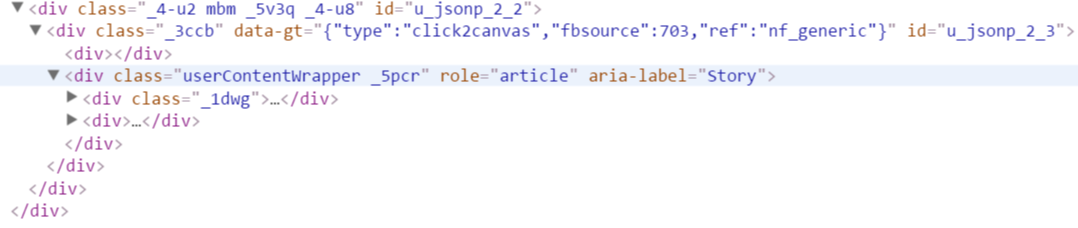
\includegraphics[width=0.9\textwidth]{facebook_html_example.png}
	\caption{Exemplo de HTML do Facebook, com algumas classes aleat�rias e algumas de nome leg�vel}
	\label{fig:facebook_html_example}
\end{figure}

A Figura \ref{fig:facebook_html_example} ilustra o que foi explicado no par�grafo anterior. Algumas das classes s�o strings aleat�rias(`{\_}5pcr', `{\_}3ccb', `{\_}1dwg', etc), enquanto que algumas possuem valores leg�veis (`userContentWrapper').

Observando estes elementos nomeados, chegou-se � seguinte estrutura simplificada para o DOM do Facebook. Todo o conte�do do site, exceto a barra azul superior e o chat que fica ao lado direito, se encontra dentro de um div chamado de mainContainer. Dentro deste mainContainer h� um div chamado de feed{\_}stream, que possui todas as postagens do feed de not�cias. O feed{\_}stream contem um ou mais substreams. Cada substream � um conjunto de postagens. Quando o usu�rio desce a p�gina at� a parte inferior, um novo substream � criado com as novas postagens. Cada substream possui uma ou mais postagens que s�o representadas por divs chamados de userContentWrapper. � poss�vel que userContentWrapper's contenham outros userContentWrapper's (por exemplo quando uma pessoa compartilha a postagem de outra pessoa). A Figura \ref{fig:facebook_dom_structure} mostra um exemplo de uma �rvore de DOM simplificada para o Facebook.

\begin{figure}[ht!]
	\centering
	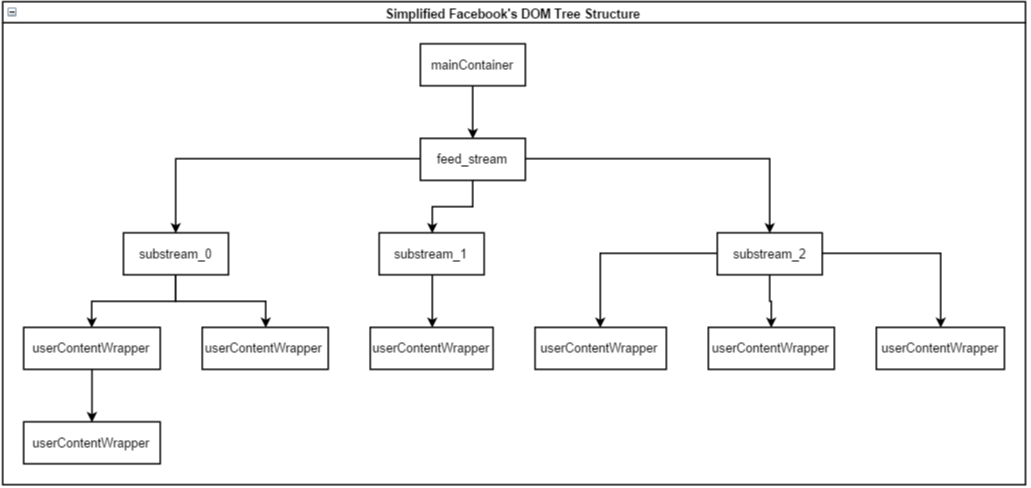
\includegraphics[width=0.9\textwidth]{facebook_dom_structure.png}
	\caption{Exemplo ilustrativo da estrutura b�sica da �rvore de DOM do Facebook}
	\label{fig:facebook_dom_structure}
\end{figure}

\subsubsection{UI desenvolvida}
A extens�o desenvolvida utiliza a API de javascript JQuery para injetar um peda�o de HTML logo acima do userContentWrapper, de modo a colocar um cabe�alho no topo de cada postagem com as classes pr� definidas. O usu�rio dever� agir como um supervisor para o classificador indicando qual o assunto da postagem em quest�o. A Figura \ref{fig:chrome_extension_header_example} ilustra o cabe�alho em uma postagem.

\begin{figure}[ht!]
	\centering
	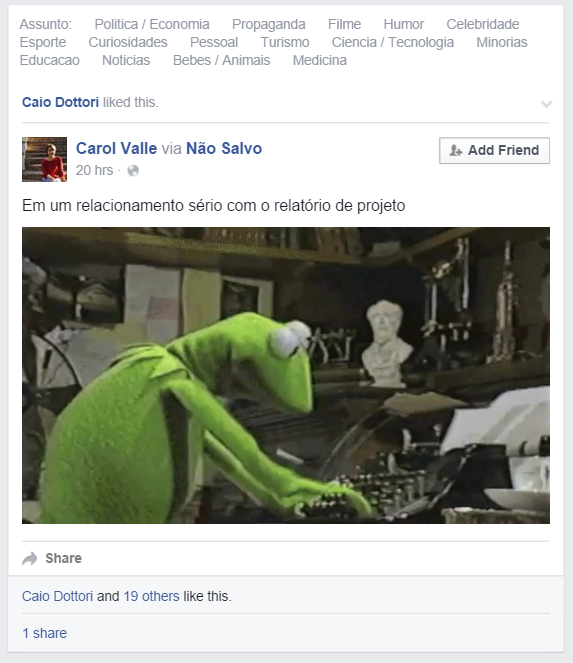
\includegraphics[width=0.9\textwidth]{chrome_extension_header_example.png}
	\caption{Exemplo em uma postagem do cabe�alho contendo as poss�veis classes}
	\label{fig:chrome_extension_header_example}
\end{figure}

Uma vez que o usu�rio clique na classe � qual a postagem pertence, o cabe�alho passa a conter apenas o nome da classe escolhida e uma barra op��es a direita que pode ser expandida, conforme a Figura \ref{fig:chrome_extension_header_classified}

\begin{figure}[ht!]
	\centering
	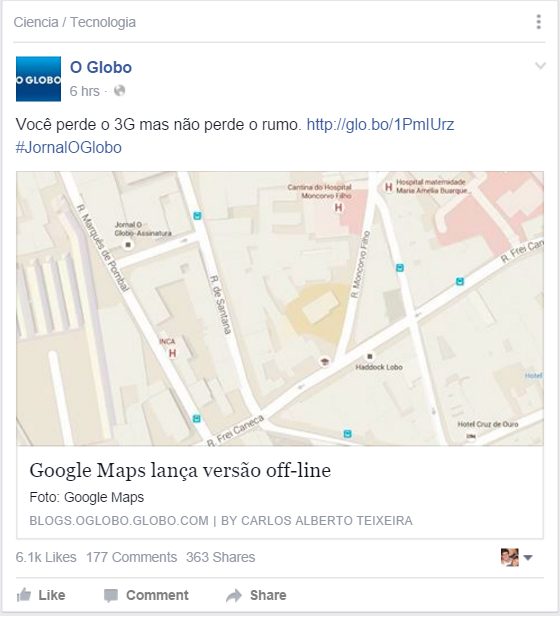
\includegraphics[width=0.9\textwidth]{chrome_extension_header_classified.png}
	\caption{Exemplo da UI de uma postagem classificada pelo usu�rio}
	\label{fig:chrome_extension_header_classified}
\end{figure}

A barra de op��es possui duas poss�veis a��es: `Mudar Assunto' ou `Adicionar Assunto'. Se o usu�rio clicar na primeira op��o ele poder� escolher um novo assunto para a postagem. Se o usu�rio clicar na segunda op��o ele poder� adicionar um novo assunto para a postagem (que ent�o possuir� duas classes). A Figura \ref{fig:barra_de_opcoes_extencao} ilustra a barra de op��es.

\begin{figure}[ht!]
	\centering
	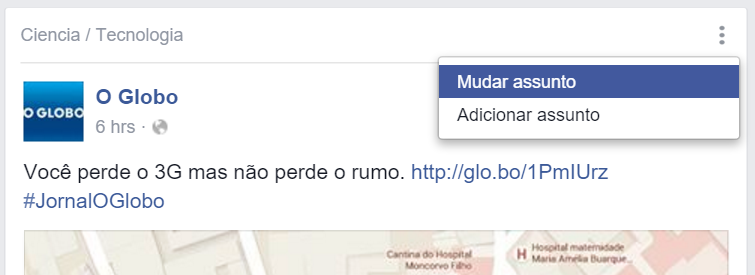
\includegraphics[width=0.9\textwidth]{barra_de_opcoes_extencao.png}
	\caption{Barra de op��es para modificar a escolha do assunto na extens�o do Chrome}
	\label{fig:barra_de_opcoes_extencao}
\end{figure}

Observe que apesar de na hora de realizar a classifica��o foi feita a simplifica��o de que o problema se trata apenas de \emph{multi-class} (n�o \emph{multi-class / multi-label}), na hora da coleta de dados � poss�vel classificar uma �nica postagem em v�rios assuntos diferentes. Isto foi feito primordialmente por dois motivos. Primeiramente, � interessante j� possuir uma base de dados com postagens com classifica��es m�ltiplas para se poder estudar o classificador \emph{multi-class / multi-label} em trabalhos futuros. Al�m disto, v�rios usu�rios diferentes podem classificar as postagens de forma distinta (n�o concordam entre si). Neste caso, o servidor guarda a contagem de classifica��es para cada classe e � considerado que a postagem pertence � classe mais frequente (empates s�o quebrados manualmente).

\subsubsection{Servidor}
Sempre que um usu�rio seleciona uma classe para uma determinada postagem, � realizada uma requisi��o POST para o servidor do Demeter (nome do projeto), contendo as informa��es relevantes. O servidor salva estas informa��es em um banco de dados.

O banco de dados contem postagens indexadas por sua url (que � um valor �nico para cada postagem) e � associado a um conjunto de classes e frequ�ncias. Por exemplo, se um post foi classificado 5 vezes como Pol�tica e 2 como educa��o, essa informa��o ficar� registrada no banco de dados.

� importante notar que n�o � apenas o texto da postagem que � salva no banco de dados. Tamb�m armazena-se o usu�rio que realizou criou a postagem, o momento em que ela foi publicada (timestamp), a presen�a de fotos ou v�deos, a exist�ncia de informa��es sobre o local de onde o usu�rio postou, etc. Essas informa��es podem ser relevantes na hora de se criar features para a NB.


\subsubsection{Crawler}

% TODO: Write about crawler

\section{Processamento do texto}
\label{sec:processamento_do_texto}

Um bom pr� processamento do texto � essencial para um bom resultado de classifica��o. Isso � especificamente v�lido em um ambiente como uma rede social, onde muitas vezes h� abrevia��es, interjei��es, utiliza��o de linguagem informal, etc.

\subsection{Tokeniza��o}
Muitas vezes as palavras puras n�o s�o muito boas para utilizar como features na classifica��o. Por isso para cada palavra associa-se um token. Este processo � chamado de tokeniza��o. Deve-se decidir o que ser� feito com a pontua��o, se palavras ser�o modificadas, etc. As vezes um token pode ser um conjunto de palavras. Por exemplo `Rio de Janeiro' pode ser um �nico token.

Outros exemplos de tokeniza��o s�o trocar todos os n�meros por um �nico token (normalmente para um classificador n�o � t�o importante o valor num�rico, mas sim a presen�a de um n�mero em si). O mesmo vale para datas, porcentagens, links, etc.

\subsection{Normaliza��o}
Normaliza��o � o processo de se criar classes de equival�ncia de palavras. Por exemplo: as palavras U.S.A e USA s�o a mesma, por�m escritas de forma diferente. Alem disso palavras possuem a primeira letra mai�scula quando iniciam uma frase ou podem estar completamente escritas em caixa alta (se o escritor quer passar a no��o de que est� gritando, por exemplo). Transformar todas as letras para caixa baixa � um tipo de normaliza��o.

\subsection{Stemming}
Stemming � o processo de trocar todas as palavras que possuem sentidos parecidos por um mesmo radical. Por exemplo, os verbos escrevo, escrevi, escrevemos, escreverei, escrevera e escreveu podem ser substitu�dos pelo radicar escrev.

\subsection{Processamento utilizado}

%TODO: Se implementarmos stemming ele tem que entrar nessa secao
Para este trabalho foram feitas as seguintes etapas de pr� processamento do texto.

\begin{itemize}
\item \textbf{Remover caracteres unicode:} Acentos, cedilhas, tremas e outros caracteres unicode s�o substitu�dos por seus equivalentes em ASCII.
\item \textbf{Remover letras mai�scula:} Todas as letras mai�sculas s�o mudadas para min�scula.
\item \textbf{Remo��o n�meros:} Quando h� um n�mero no texto, seu valor exato n�o importa muito para o classificador. O que importa � a sua presen�a. O mesmo vale para datas, porcentagens, urls, valores de dinheiro e datas. No caso, os n�meros s�o substitu�dos por `\{number\}', as datas por `\{date\}' e assim por diante.
\item \textbf{Remover a pontua��o:} Toda a pontua��o � removida.
\item \textbf{Encontrar risadas:} Todas as ocorr�ncias de risadas (que puderam ser identificadas com algumas heur�sticas simples) s�o substitu�das por `{laughter}'
\item \textbf{Remover letras duplas:} Em redes sociais � muito comum o usu�rio repetir a mesma letras diversas vezes para enfatizar a palavra. Por exemplo: `Que FOOOOOOOOOOFO!'. Isto atrapalharia o classificador. Por isso letras repetidas s�o removidas. Note que, apesar de ser permitido no portugu�s `r' e `s' duplos, remov�-los n�o atrapalhar� muito o classificador.
\item \textbf{Filtrar palavras comuns e que n�o agregam muito valor ao classificador:} Palavras comuns do portugu�s como artigos, preposi��es, etc, s�o desconsideradas.
\end{itemize} 

\section{Tecnologias utilizadas}

Para o desenvolvimento deste projeto, foram utilizadas diversas tecnologias e ferramentas computacionais diferentes.

O versionamento de c�digo foi feito utilizando o Git, com reposit�rio p�blico hospedado no Github.

Para se desenvolver a extens�o do Chrome utilizou-se o framework disponibilizado pelo pr�prio Google. As linguagens adotadas para tal foram Javascript, HTML e CSS.

O servidor foi feito no Google App Engine, que permite a utiliza��o da infraestrutura do Google de forma gratuita e simples. O utilizou-se a API do NDB para o gerenciamento do banco de dados.

O classificador foi inteiramente desenvolvido em Python 2.7 por conta de sua versatilidade e facilidade de programa��o.


\chapter{Proposta de Classificador}
\label{sec:proposta_de_classificador}

\externaldocument{fundamentacao_teorica}
\externaldocument{metodologia}

Foram propostas diversas formas diferentes de classificadores, e cada uma ser� posteriormente avaliada e comparada.

\section{Classes adotadas}
\label{ref:classes_adotadas}
Foram consideradas as seguintes classes para todos os classificadores desenvolvidos:

\begin{itemize}
	\item Politica / Economia 
	\item Propaganda
	\item Filmes / Series
	\item Humor
	\item Celebridade
	\item Esporte
	\item Pessoal
	\item Turismo
	\item Ciencia / Tecnologia / Meio Ambiente
	\item Minorias
	\item Educacao
	\item Noticias
	\item Bebes / Animais
	\item Saude
\end{itemize}

\section{Na�ve Bayes utilizando apenas o texto}
O classificador mais simples que pode ser criado utilizando NB, consiste em utilizar apenas as palavras do texto como features. 

Neste caso, realizou-se primeiramente o processamento conforme o descrito na Se��o \ref{sec:processamento_do_texto}, normalizando as palavras de forma apropriada. Durante o processo de normaliza��o, foram realizadas as seguintes modifica��es.

\begin{itemize}
	\item Todos os links foram trocados pelo token '\{link\}'
	\item Todas as refer�ncias feitas com @ (por exemplo @NomeDaPessoa) foram trocadas pelo token '\{tag\}'
	\item Todos os valores monet�rios (tanto em real como em d�lar) foram trocados pelo token '{money}'
	\item Todas as percentagens foram trocadas pelo token '\{percentage\}'
	\item Todas as datas foram trocadas pelo token '\{date\}'
	\item Todos os outros n�meros foram trocados pelo token '\{number\}'
\end{itemize}

Em seguida, realizou-se o treinamento utilizando base de dados obtida, realizando-se a contagem da ocorr�ncia dos tokens em cada uma das classes. Finalmente testou-se a performance do classificador obtido em um conjunto de testes.

\section{Na�ve Bayes com Features Adicionais}
\label{sec:bayes_features_adicionais}
V�rias outras features foram adicionadas na tentativa de melhorar a performance do classificador. As postagens em redes sociais em geral contem muito mais informa��es do que o texto escrito. Tentaram-se captur�-las utilizando as seguintes features:

\begin{itemize}
	\item Usu�rio ou p�gina que � autor(a) da postagem
	\item Tipo de compartilhamento (se � apenas um status update, ou se � um v�deo ou uma foto que est�o sendo compartilhados)
	\item Se a postagem possui uma localiza��o de origem (o valor do local em si de onde a postagem foi feita n�o foi considerado, pois seria necess�ria uma base de dados muito grande para que este local fizesse diferen�a)
	\item Se h� algum outro usu�rio marcado na postagem (considerou-se esta feature interessante pelo fato de que postagens pessoas costumam ter pessoas marcadas).
	\item Se a postagem foi promovida por meio de pagamentos (tem a tag Sponsor no Facebook) ou n�o
	\item O tamanho do texto (discretizou-se o tamanho em 4 categorias: tiny, small, medium, large)
\end{itemize}

� importante notar que o ideal seria recuperar informa��es a partir das imagens e v�deos compartilhados, entretanto este problema foge ao escopo deste trabalho.



\section{Weighted Na�ve Bayes utilizando apenas o texto}
Utilizaram-se as Weighted Na�ve Bayes descritas na Se��o \ref{sec:weighted_naive_bayes} para ponderar a import�ncia das features relevando a no��o independ�ncia condicional das NBs.

\section{Weighted Na�ve Bayes com Features Adicionais}

Repetiu-se a mesma ideia exposta na Se��o \ref{sec:bayes_features_adicionais}, porem desta vez com a NB ponderada.

\section{Utiliza��o dos links}
At� agora, o conte�do dos links compartilhados tinha sido completamente ignorado. Por exemplo, se algu�m postasse um link sobre economia e escrevesse algo do tipo `Muito interessante esta an�lise', o classificador iria tentar classificar a potagem utilizando apenas o texto (o que � bem complicado). Para evitar este problema, fez-se um HTTP GET request para o link, extraiu-se o texto principal e ele foi classificado por um segundo classificador. O resultado deste segundo classificador passa a ser uma feature do classificador de postagens.

Este segundo classificador (que ser� referenciado como classificador de artigos) foi treinado a partir da base de dados adquirida pelo crawler.
 
\section{Concatena��o do texto dos links}
% TODO: Falar da concatena��o do texto dos links no post (se a gente efetivamente fizer isto)
% Uma outra abordagem utilizada foi a de concatenar o texto contido no link com o texto da postagem. Desta forma ambos s�o treinados e classificados simultaneamente.

\section{Fus�o de classes pequenas}
% TODO: Falar das classes pouco frequentes
% Uma outra mudan�a considerada para melhorar a qualidade do classificador foi a fus�o de classes pequenas.

% Muitas das classes consideradas n�o s�o t�o recorrentes no Facebook dos supervisores e portanto conseguiram poucos exemplos para os conjuntos de treinamento e teste. Isto faz com que o classificador n�o possua informa��o suficiente para realizar a classifica��o de forma adequada.

% Al�m disso, existem algumas classes que possuem dom�nios bem proximos que, muitas vezes, s�o de dif�cil distin��o at� para um ser humado (cita-se como exemplo `Celebridades' vs `Filmes'). Isto tambem aumenta a taxa de errodo classificador.

% A solu��o adotada foi a fus�o destas classes em outra mais abrangentes.


\chapter{Tecnologias Utilizadas}
\input{tecnologias_utilizadas}

\chapter{Valida��o - Experimentos, resultados e an�lise}
\externaldocument{metodologia}
\externaldocument{fundamentacao_teorica}
\externaldocument{proposta_de_classificador}

\section{Base de dados}
A base de dados para a classifica��o de postagens foi adquirida a partir da extens�o do Chrome descrita na Se��o \ref{sec:plugin_chrome}. A classifica��o foi feita manualmente por diversos supervisores, classificando cada postagem nas diferentes categorias explicitadas na Se��o \ref{ref:classes_adotadas}. 

O gr�fico da Figura \ref{fig:classes_freq} ilustra a propor��o entre as diferentes classes na base de dados obtida.

\begin{figure}[ht!]
	\centering
	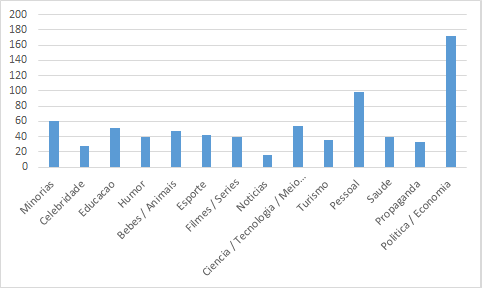
\includegraphics[width=0.9\textwidth]{classes_freq.png}
	\caption{Histograma representativo da base de dados de postagens adquirida}
	\label{fig:classes_freq}
\end{figure}

A menor base � de `Not�cias', com apenas 16 postagens, e a maior � `Pol�tica / Economia' com 172 postagens. O total de postagens � 757. Observa-se que este n�o � um n�mero muito grande para uma base de dados, ainda mais com um total de 14 classes, mas foi o que foi poss�vel de se adquirir.

\section{Na�ve Bayes utilizando apenas o texto}

Nesta primeira abordagem, o classificador obteve uma acur�cia m�dia (ao longo de 100 parti��es aleat�rias diferentes da base de dados em treinamento e valida��o, conforme o explicado na Se��o \ref{sec:validacao}) de 49.7\%, ou seja, o classificador acerta basicamente 1 a cada 2 postagens. Como j� foi dito na Se��o \ref{sec:acuracia}, a acur�cia � uma m�trica bem ruim para avaliar um classifiador. Desta forma, foram consideradas as outras estat�sticas explicadas no cap�tulo de metodologia, para uma an�lise mais profunda.

A acur�cia esperada para este classificador, utilizando a Equa��o \ref{eq:acuracia_esperada}, � de 14.16\%. O $Kappa$ neste caso foi de 41.4\%. Segundo o benchmark de Landis e Koch \cite{landis1977measurement}, trata-se de um resultado moderado. Note que a estat�stica $Kappa$ agrega muito mais informa��o que uma simples acur�cia.

� interessante observar como o Kappa e a acur�cia variam conforme se aumenta o tamanho da base de dado. Para tal, repetiu-se o processo de treinamento e valida��o com a base de dados de tamanho vari�vel (pegando-se subconjuntos aleat�rios da base de dados original). Manteve-se sempre uma propor��o de 75\% pra treinamento e 25\% para valida��o. A Figura \ref{fig:nb_apenas_com_texto_accuracy_graph} mostra o crescimento da acur�cia, enquanto que a Figura \ref{fig:nb_apenas_com_texto_kappa_graph} mostra o crescimento do Kappa.

\begin{figure}[ht!]
	\centering	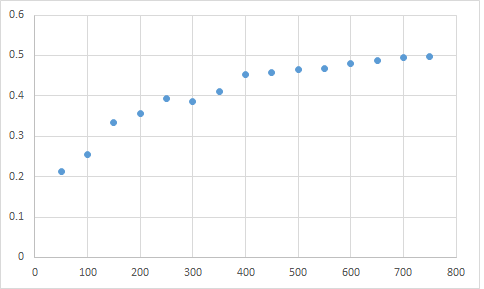
\includegraphics[width=0.9\textwidth]{nb_apenas_com_texto_accuracy_graph.png}
	\caption{Acur�cia em fun��o da quantidade de postagens na base de dados (treinamento + valida��o) para NB simples}
	\label{fig:nb_apenas_com_texto_accuracy_graph}
\end{figure}

\begin{figure}[ht!]
	\centering	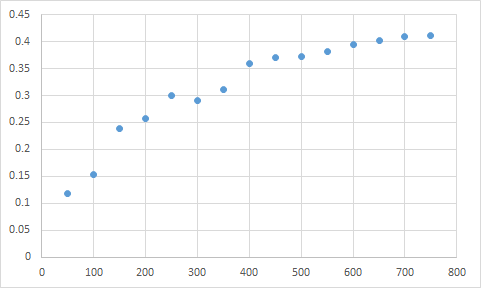
\includegraphics[width=0.9\textwidth]{nb_apenas_com_texto_kappa_graph.png}
	\caption{Kappa em fun��o da quantidade de postagens na base de dados (treinamento + valida��o) para NB simples}
	\label{fig:nb_apenas_com_texto_kappa_graph}
\end{figure}

Para se compreender onde exatamente o classificador est� ruim, rodou-se novamente o programa com apenas uma itera��o e construiu-se a matriz de confus�o para os resultados obtidos, como pode ser visto na Tabela \ref{tab:nb_apenas_com_o_texto}.

Para este exemplo tem-se:

$acuracia=0.529101$

$acuracia\_esperada=0.138154$

$Kappa=0.453615$


A Tabela \ref{tab:nb_apenas_com_o_texto} apresenta a matriz de confusao.


\begin{table}[tph]
	\begin{center}
		\begin{tabular}{ c  c  c  c  c  c  c  c  c  c  c  c  c  c }
			\hline
			Beb & Cel & Cie & Edu & Esp & Fil & Hum & Min & Not & Pes & Pol & Pro & Sau & Tur\\
			\hline
			7 & 0 & 1 & 0 & 0 & 0 & 0 & 0 & 0 & 1 & 0 & 2 & 0 & 0\\
			0 & 1 & 0 & 0 & 0 & 1 & 0 & 0 & 0 & 0 & 0 & 0 & 0 & 0\\
			0 & 1 & 2 & 0 & 0 & 0 & 1 & 0 & 0 & 0 & 1 & 0 & 0 & 0\\
			0 & 0 & 2 & 8 & 0 & 1 & 1 & 0 & 0 & 0 & 1 & 0 & 1 & 0\\
			0 & 0 & 0 & 1 & 5 & 0 & 0 & 0 & 0 & 0 & 0 & 1 & 0 & 0\\
			0 & 0 & 1 & 0 & 0 & 4 & 1 & 0 & 0 & 1 & 0 & 0 & 0 & 0\\
			0 & 0 & 1 & 0 & 0 & 0 & 1 & 0 & 0 & 0 & 0 & 0 & 0 & 0\\
			0 & 1 & 1 & 1 & 0 & 1 & 1 & 9 & 1 & 3 & 2 & 1 & 0 & 1\\
			0 & 0 & 0 & 0 & 0 & 0 & 0 & 0 & 0 & 0 & 0 & 0 & 0 & 0\\
			3 & 3 & 0 & 1 & 2 & 0 & 0 & 1 & 0 & 21 & 0 & 3 & 0 & 1\\
			1 & 1 & 4 & 2 & 2 & 1 & 7 & 4 & 3 & 1 & 38 & 2 & 4 & 1\\
			0 & 1 & 1 & 0 & 0 & 0 & 0 & 0 & 0 & 0 & 0 & 0 & 0 & 1\\
			0 & 0 & 0 & 0 & 0 & 0 & 0 & 0 & 1 & 0 & 1 & 2 & 1 & 2\\
			0 & 0 & 0 & 0 & 0 & 0 & 0 & 0 & 0 & 0 & 0 & 0 & 0 & 3\\
			\hline
		\end{tabular}
	\end{center}
	\caption{Matriz de confusao para a NB apenas com o texto}
	\label{tab:nb_apenas_com_o_texto}
\end{table}


A Figura \ref{fig:nb_apenas_com_o_texto} consiste numa representa��o gr�fica da matriz de confus�o.

\begin{figure}[ht!]
	\centering	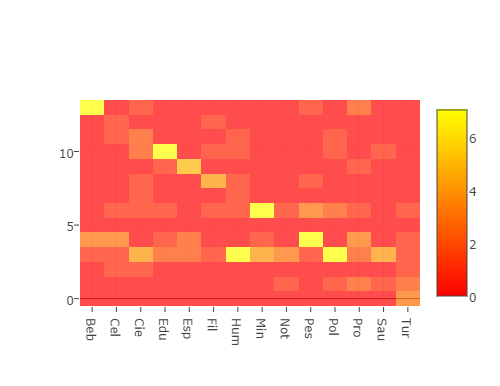
\includegraphics[width=0.9\textwidth]{nb_apenas_com_o_texto.png}
	\caption{Heatmap da matriz de confus�o da Tabela \ref{tab:nb_apenas_com_o_texto}}
	\label{fig:nb_apenas_com_o_texto}
\end{figure}

Outras estat�sticas analisadas s�o as precis�es, as abrang�ncias e os f1scores para cada uma das classes, conforme relacionado na Tabela \ref{tab:nb_apenas_com_o_texto_prec_rec}.

\begin{table}[tph]
	\begin{center}
		\begin{tabular}{ c  c  c  c }
			\hline
			Classe & Precisao & Abrangencia & F1score \\
			\hline
			Bebes & 0.636364 & 0.636364 & 0.636364 \\
			Celebridade & 0.500000 & 0.125000 & 0.200000 \\
			Ciencia & 0.400000 & 0.153846 & 0.222222 \\
			Educacao & 0.571429 & 0.615385 & 0.592593 \\
			Esporte & 0.714286 & 0.555556 & 0.625000 \\
			Filmes & 0.571429 & 0.500000 & 0.533333 \\
			Humor & 0.500000 & 0.083333 & 0.142857 \\
			Minorias & 0.409091 & 0.642857 & 0.500000 \\
			Noticias & 1.000000 & 0.000000 & 1.000000 \\
			Pessoal & 0.600000 & 0.777778 & 0.677419 \\
			Politica & 0.535211 & 0.883721 & 0.666667 \\
			Propaganda & 0.000000 & 1.000000 & 0.000000 \\
			Saude & 0.142857 & 0.166667 & 0.153846 \\
			Turismo & 1.000000 & 0.333333 & 0.500000 \\
			Media Micro & 0.529101 & 0.529101 & 0.529101 \\
			Media Macro & 0.541476 & 0.462417 & 0.498833 \\
			\hline
		\end{tabular}
	\end{center}
	\caption{Precis�o e abrangencia para NB apenas com o texto}
	\label{tab:nb_apenas_com_o_texto_prec_rec}
\end{table}


\section{Na�ve Bayes com Features Adicionais}
% Isso piora o classificador pois adiciona redundancia (e quebra a nocao de independencia condicional)

% citar a secao que explica essas features

A acur�cia m�dia obtida depois da adi��o das features extras foi de 51.1\%. A m�trica Kappa foi de 42.5\%. Observa-se portanto que houve uma pequena melhora em rela��o as redes Bayesianas com o texto puro(o Kappa variou de 41.4\% para 42.5\%). 

O motivo da melhoria ser t�o pequena � que ocorrem dois efeitos opostos quando se adicionam essas novas features. Por um lado, essas novas features adicionam novas informa��es que possibilitam que haja uma melhor classifica��o. Por outro lado, essas novas features s�o muitas vezes dependentes condicionalmente das palavras do texto. Como as NB assumem, independ�ncia condicional, a adi��o de features dependentes pode piorar a rede. O resultado da soma desses dois efeitos foi ligeiramente positivo neste caso.

A Figura \ref{fig:nb_features_extras_accuracy_graph} abaixo mostra a evolu��o da acur�cia das NB com features extras em fun��o do tamanho da base de dados. A Figura \ref{fig:nb_features_extras_kappa_graph} mostra a rela��o do Kappa com o tamanho da base de dados. A Figura \ref{fig:nb_features_extras_vs_apenas_texto_kappa_graph} compara os gr�ficos do Kappa para as NB com e sem features extras.

\begin{figure}[ht!]
	\centering	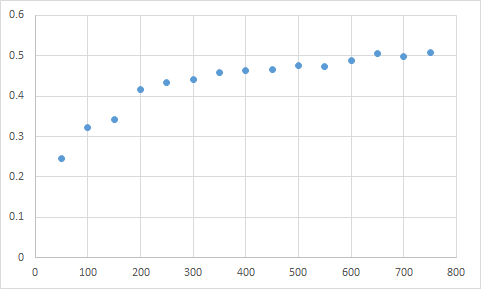
\includegraphics[width=0.9\textwidth]{nb_features_extras_accuracy_graph.png}
	\caption{Acur�cia em fun��o da quantidade de postagens na base de dados (treinamento + valida��o) para NB com features extras (alem das palavras do texto)}
	\label{fig:nb_features_extras_accuracy_graph}
\end{figure}


\begin{figure}[ht!]
	\centering	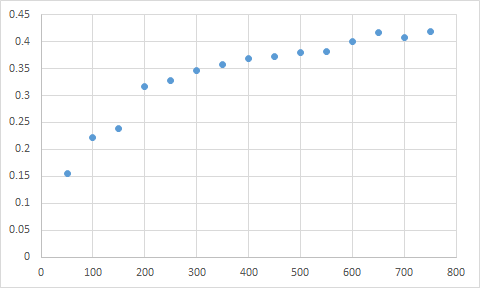
\includegraphics[width=0.9\textwidth]{nb_features_extras_kappa_graph.png}
	\caption{Kappa em fun��o da quantidade de postagens na base de dados (treinamento + valida��o) para NB com features extras (alem das palavras do texto)}
	\label{fig:nb_features_extras_kappa_graph}
\end{figure}

\begin{figure}[ht!]
	\centering	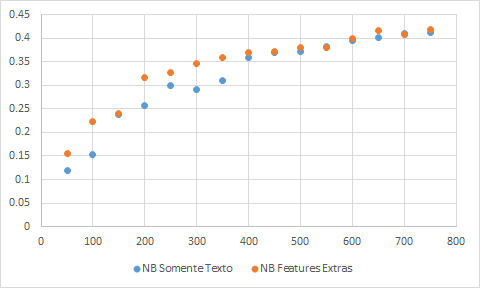
\includegraphics[width=0.9\textwidth]{nb_features_extras_vs_apenas_texto_kappa_graph.png}
	\caption{Sobreposi��o dos gr�ficos do Kappa em fun��o da quantidade de postagens na base de dados para NB com e sem as features extras}
	\label{fig:nb_features_extras_vs_apenas_texto_kappa_graph}
\end{figure}

Para este exemplo tem-se:

$acuracia=0.513228$

$acuracia\_esperada=0.140058$

$Kappa=0.433948$


A Tabela \ref{tab:nb_com_features_adicionais} apresenta a matriz de confusao.


\begin{table}[tph]
	\begin{center}
		\begin{tabular}{ c  c  c  c  c  c  c  c  c  c  c  c  c  c }
			\hline
			Beb & Cel & Cie & Edu & Esp & Fil & Hum & Min & Not & Pes & Pol & Pro & Sau & Tur\\
			\hline
			6 & 0 & 0 & 0 & 0 & 0 & 1 & 0 & 0 & 0 & 0 & 0 & 0 & 1\\
			0 & 0 & 0 & 0 & 0 & 0 & 0 & 0 & 0 & 0 & 0 & 0 & 0 & 0\\
			0 & 1 & 3 & 0 & 0 & 1 & 0 & 0 & 1 & 0 & 0 & 1 & 1 & 0\\
			0 & 0 & 3 & 3 & 1 & 0 & 0 & 0 & 0 & 0 & 0 & 1 & 0 & 0\\
			0 & 0 & 0 & 0 & 1 & 0 & 0 & 0 & 0 & 0 & 0 & 0 & 0 & 0\\
			0 & 0 & 0 & 0 & 0 & 3 & 0 & 0 & 0 & 0 & 0 & 0 & 0 & 0\\
			0 & 0 & 0 & 0 & 0 & 0 & 5 & 0 & 0 & 0 & 0 & 0 & 0 & 0\\
			1 & 0 & 0 & 2 & 1 & 1 & 0 & 6 & 2 & 1 & 1 & 0 & 1 & 0\\
			0 & 0 & 0 & 0 & 0 & 0 & 0 & 0 & 0 & 0 & 0 & 0 & 0 & 0\\
			4 & 3 & 0 & 3 & 6 & 3 & 4 & 2 & 1 & 22 & 1 & 1 & 1 & 2\\
			0 & 2 & 2 & 4 & 1 & 2 & 2 & 5 & 5 & 2 & 39 & 0 & 7 & 0\\
			0 & 0 & 1 & 0 & 1 & 3 & 0 & 0 & 0 & 0 & 0 & 3 & 0 & 1\\
			0 & 0 & 0 & 0 & 0 & 0 & 0 & 0 & 0 & 0 & 1 & 0 & 2 & 0\\
			0 & 0 & 0 & 0 & 0 & 0 & 0 & 0 & 0 & 0 & 0 & 0 & 0 & 4\\
			\hline
		\end{tabular}
	\end{center}
	\caption{Matriz de confusao para a NB com features adicionais}
	\label{tab:nb_com_features_adicionais}
\end{table}


A Figura \ref{fig:nb_com_features_adicionais} consiste numa representa��o gr�fica da matriz de confus�o.

\begin{figure}[ht!]
	\centering	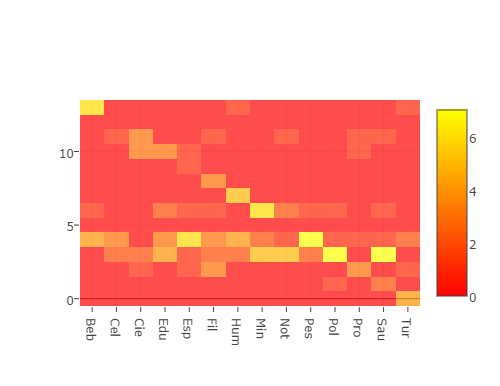
\includegraphics[width=0.9\textwidth]{nb_com_features_adicionais.png}
	\caption{Heatmap da matriz de confus�o da Tabela \ref{tab:nb_com_features_adicionais}}
	\label{fig:nb_com_features_adicionais}
\end{figure}

Outras estat�sticas analisadas s�o as precis�es, as abrang�ncias e os f1scores para cada uma das classes, conforme relacionado na Tabela \ref{tab:nb_com_features_adicionais_prec_rec}.

\begin{table}[tph]
	\begin{center}
		\begin{tabular}{ c  c  c  c }
			\hline
			Classe & Precisao & Abrangencia & F1score \\
			\hline
			Bebes & 0.750000 & 0.545455 & 0.631579 \\
			Celebridade & 1.000000 & 0.000000 & 0.000000 \\
			Ciencia & 0.375000 & 0.333333 & 0.352941 \\
			Educacao & 0.375000 & 0.250000 & 0.300000 \\
			Esporte & 1.000000 & 0.090909 & 0.166667 \\
			Filmes & 1.000000 & 0.230769 & 0.375000 \\
			Humor & 1.000000 & 0.416667 & 0.588235 \\
			Minorias & 0.375000 & 0.461538 & 0.413793 \\
			Noticias & 1.000000 & 0.000000 & 0.000000 \\
			Pessoal & 0.415094 & 0.880000 & 0.564103 \\
			Politica & 0.549296 & 0.928571 & 0.690265 \\
			Propaganda & 0.333333 & 0.500000 & 0.400000 \\
			Saude & 0.666667 & 0.166667 & 0.266667 \\
			Turismo & 1.000000 & 0.500000 & 0.666667 \\
			Media Micro & 0.513228 & 0.513228 & 0.513228 \\
			Media Macro & 0.702814 & 0.378850 & 0.492317 \\
			\hline
		\end{tabular}
	\end{center}
	\caption{Precis�o e abrangencia para NB com features adicionais}
	\label{tab:nb_com_features_adicionais_prec_rec}
\end{table}


\section{Weighted Na�ve Bayes utilizando apenas o texto}
%notar que apesar da acuracia ter melhorado pouco, o Kappa melhorou muito

A acur�cia m�dia obtida, depois da adi��o de pesos nas features e utilizando apenas as palavras do texto, foi de 53.5\%. A m�trica Kappa foi de 48.2\%. Observa-se portanto que houve uma melhora consider�vel na m�trica Kappa em rela��o �s abordagens anteriores e uma melhora pequena na acur�cia.

\begin{figure}[ht!]
	\centering	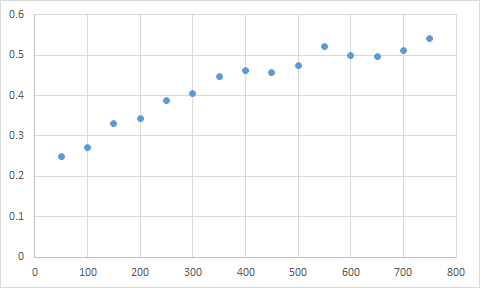
\includegraphics[width=0.9\textwidth]{wnb_somente_texto_accuracy_graph.png}
	\caption{Acur�cia em fun��o da quantidade de postagens na base de dados (treinamento + valida��o) para a Weighted NB utilizando apenas o texto}
	\label{fig:wnb_somente_texto_accuracy_graph}
\end{figure}


\begin{figure}[ht!]
	\centering	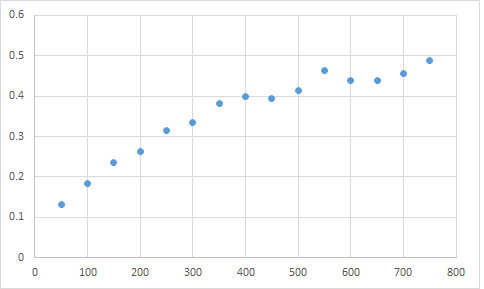
\includegraphics[width=0.9\textwidth]{wnb_somente_texto_kappa_graph.png}
	\caption{Kappa em fun��o da quantidade de postagens na base de dados (treinamento + valida��o) para a Weighted NB utilizando apenas o texto}
	\label{fig:wnb_somente_texto_kappa_graph}
\end{figure}

\begin{figure}[ht!]
	\centering	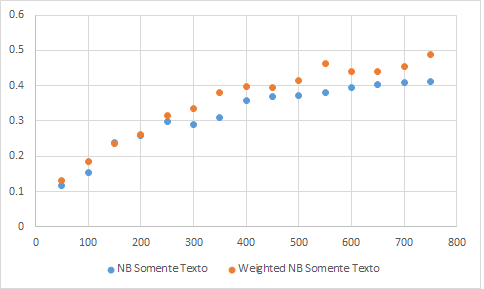
\includegraphics[width=0.9\textwidth]{nb_somente_texto_vs_wnb_kappa_graph.png}
	\caption{Sobreposi��o dos gr�ficos do Kappa em fun��o da quantidade de postagens na base de dados para o NB Simples e o Weighted NB}
	\label{fig:nb_somente_texto_vs_wnb_kappa_graph}
\end{figure}

Para este exemplo tem-se:

$acuracia=0.544974$

$acuracia\_esperada=0.104000$

$Kappa=0.492158$


A Tabela \ref{tab:weighted_nb_apenas_com_texto} apresenta a matriz de confusao.


\begin{table}[tph]
	\begin{center}
		\begin{tabular}{ c  c  c  c  c  c  c  c  c  c  c  c  c  c }
			\hline
			Beb & Cel & Cie & Edu & Esp & Fil & Hum & Min & Not & Pes & Pol & Pro & Sau & Tur\\
			\hline
			7 & 0 & 1 & 0 & 0 & 1 & 0 & 2 & 0 & 1 & 0 & 1 & 0 & 0\\
			0 & 1 & 0 & 0 & 1 & 0 & 0 & 0 & 0 & 0 & 0 & 0 & 0 & 0\\
			0 & 0 & 6 & 1 & 0 & 0 & 1 & 0 & 0 & 0 & 1 & 0 & 1 & 1\\
			1 & 0 & 3 & 8 & 1 & 0 & 0 & 1 & 0 & 0 & 2 & 1 & 2 & 0\\
			0 & 0 & 0 & 0 & 8 & 0 & 0 & 0 & 0 & 0 & 2 & 1 & 0 & 0\\
			0 & 1 & 0 & 0 & 0 & 12 & 0 & 0 & 0 & 1 & 2 & 1 & 0 & 2\\
			0 & 0 & 0 & 0 & 0 & 0 & 2 & 0 & 0 & 0 & 0 & 0 & 0 & 0\\
			2 & 1 & 1 & 1 & 0 & 0 & 2 & 9 & 1 & 4 & 12 & 0 & 0 & 2\\
			0 & 0 & 0 & 0 & 0 & 0 & 0 & 0 & 0 & 0 & 0 & 0 & 0 & 0\\
			1 & 0 & 0 & 0 & 2 & 0 & 1 & 1 & 0 & 12 & 0 & 0 & 0 & 1\\
			1 & 2 & 0 & 1 & 0 & 1 & 3 & 0 & 0 & 2 & 24 & 0 & 2 & 1\\
			0 & 0 & 0 & 1 & 0 & 1 & 1 & 1 & 0 & 0 & 1 & 3 & 0 & 0\\
			0 & 0 & 0 & 0 & 0 & 0 & 0 & 0 & 0 & 0 & 0 & 0 & 6 & 0\\
			0 & 0 & 0 & 1 & 1 & 0 & 0 & 0 & 0 & 0 & 1 & 0 & 0 & 5\\
			\hline
		\end{tabular}
	\end{center}
	\caption{Matriz de confusao para a Weighted NB apenas com texto}
	\label{tab:weighted_nb_apenas_com_texto}
\end{table}


A Figura \ref{fig:weighted_nb_apenas_com_texto} consiste numa representa��o gr�fica da matriz de confus�o.

\begin{figure}[ht!]
	\centering	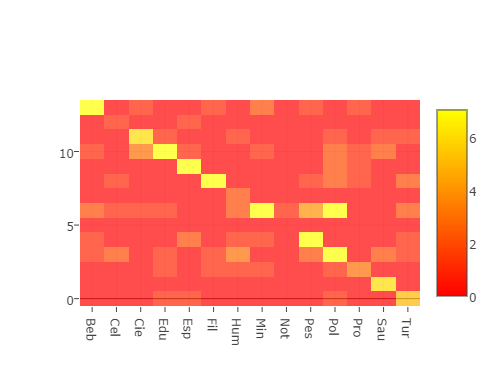
\includegraphics[width=0.9\textwidth]{weighted_nb_apenas_com_texto.png}
	\caption{Heatmap da matriz de confus�o da Tabela \ref{tab:weighted_nb_apenas_com_texto}}
	\label{fig:weighted_nb_apenas_com_texto}
\end{figure}

Outras estat�sticas analisadas s�o as precis�es, as abrang�ncias e os f1scores para cada uma das classes, conforme relacionado na Tabela \ref{tab:weighted_nb_apenas_com_texto_prec_rec}.

\begin{table}[tph]
	\begin{center}
		\begin{tabular}{ c  c  c  c }
			\hline
			Classe & Precisao & Abrangencia & F1score \\
			\hline
			Bebes & 0.538462 & 0.583333 & 0.560000 \\
			Celebridade & 0.500000 & 0.200000 & 0.285714 \\
			Ciencia & 0.545455 & 0.545455 & 0.545455 \\
			Educacao & 0.421053 & 0.615385 & 0.500000 \\
			Esporte & 0.727273 & 0.615385 & 0.666667 \\
			Filmes & 0.631579 & 0.800000 & 0.705882 \\
			Humor & 1.000000 & 0.200000 & 0.333333 \\
			Minorias & 0.257143 & 0.642857 & 0.367347 \\
			Noticias & 1.000000 & 0.000000 & 0.000000 \\
			Pessoal & 0.666667 & 0.600000 & 0.631579 \\
			Politica & 0.648649 & 0.533333 & 0.585366 \\
			Propaganda & 0.375000 & 0.428571 & 0.400000 \\
			Saude & 1.000000 & 0.545455 & 0.705882 \\
			Turismo & 0.625000 & 0.416667 & 0.500000 \\
			Media Micro & 0.544974 & 0.544974 & 0.544974 \\
			Media Macro & 0.638306 & 0.480460 & 0.548248 \\
			\hline
		\end{tabular}
	\end{center}
	\caption{Precis�o e abrangencia para Weighted NB apenas com texto}
	\label{tab:weighted_nb_apenas_com_texto_prec_rec}
\end{table}


\section{Weighted Na�ve Bayes com Features Adicionais}
% Nesse caso nao tem problema adicionar features redundantes pois os pesos aliviam a hipotese de independencia condicional

\begin{figure}[ht!]
	\centering	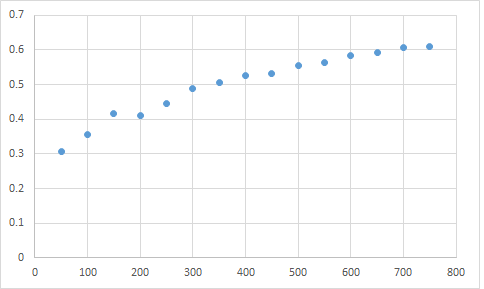
\includegraphics[width=0.9\textwidth]{wnb_features_extras_accuracy_graph.png}
	\caption{Acur�cia em fun��o da quantidade de postagens na base de dados (treinamento + valida��o) para a Weighted NB com features extras}
	\label{fig:wnb_features_extras_accuracy_graph}
\end{figure}


\begin{figure}[ht!]
	\centering	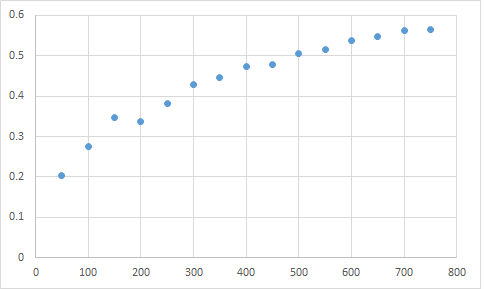
\includegraphics[width=0.9\textwidth]{wnb_features_extras_kappa_graph.png}
	\caption{Kappa em fun��o da quantidade de postagens na base de dados (treinamento + valida��o) para a Weighted NB com features extras}
	\label{fig:wnb_features_extras_kappa_graph}
\end{figure}

\begin{figure}[ht!]
	\centering	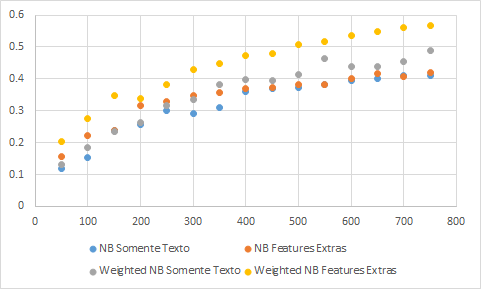
\includegraphics[width=0.9\textwidth]{nb_vs_wnb.png}
	\caption{Compara��o dos quatro classificadores propostos, mostrando o Kappa de cada um como uma fun��o do tamanho da base de dados.}
	\label{fig:nb_vs_wnb}
\end{figure}


Para este exemplo tem-se:

$acuracia=0.656085$

$acuracia\_esperada=0.108060$

$Kappa=0.614419$


A Tabela \ref{tab:weighted_nb_com_features_extras} apresenta a matriz de confusao.


\begin{table}[tph]
	\begin{center}
		\begin{tabular}{ c  c  c  c  c  c  c  c  c  c  c  c  c  c }
			\hline
			Beb & Cel & Cie & Edu & Esp & Fil & Hum & Min & Not & Pes & Pol & Pro & Sau & Tur\\
			\hline
			5 & 1 & 1 & 1 & 0 & 0 & 0 & 0 & 0 & 0 & 0 & 1 & 0 & 0\\
			0 & 3 & 0 & 0 & 0 & 0 & 0 & 0 & 0 & 0 & 0 & 0 & 0 & 0\\
			0 & 0 & 6 & 0 & 0 & 0 & 0 & 0 & 1 & 1 & 1 & 0 & 0 & 0\\
			0 & 0 & 5 & 7 & 1 & 1 & 0 & 3 & 0 & 0 & 4 & 1 & 1 & 0\\
			0 & 0 & 1 & 0 & 7 & 0 & 0 & 0 & 0 & 0 & 0 & 0 & 0 & 1\\
			0 & 0 & 0 & 1 & 0 & 7 & 0 & 0 & 0 & 0 & 0 & 1 & 1 & 0\\
			0 & 0 & 0 & 0 & 0 & 0 & 5 & 0 & 0 & 0 & 0 & 0 & 0 & 0\\
			2 & 1 & 0 & 0 & 0 & 0 & 0 & 14 & 2 & 0 & 5 & 0 & 1 & 0\\
			0 & 0 & 0 & 0 & 0 & 0 & 0 & 0 & 1 & 0 & 1 & 0 & 0 & 0\\
			2 & 1 & 0 & 0 & 0 & 0 & 0 & 1 & 0 & 24 & 1 & 2 & 0 & 2\\
			1 & 0 & 0 & 0 & 0 & 1 & 0 & 1 & 0 & 0 & 30 & 0 & 1 & 1\\
			0 & 0 & 1 & 1 & 0 & 1 & 0 & 0 & 0 & 1 & 1 & 4 & 0 & 0\\
			0 & 0 & 0 & 1 & 0 & 1 & 0 & 0 & 1 & 0 & 2 & 0 & 6 & 0\\
			0 & 1 & 0 & 0 & 0 & 0 & 0 & 0 & 0 & 0 & 0 & 0 & 0 & 5\\
			\hline
		\end{tabular}
	\end{center}
	\caption{Matriz de confusao para a Weighted NB com features extras}
	\label{tab:weighted_nb_com_features_extras}
\end{table}


A Figura \ref{fig:weighted_nb_com_features_extras} consiste numa representa��o gr�fica da matriz de confus�o.

\begin{figure}[ht!]
	\centering	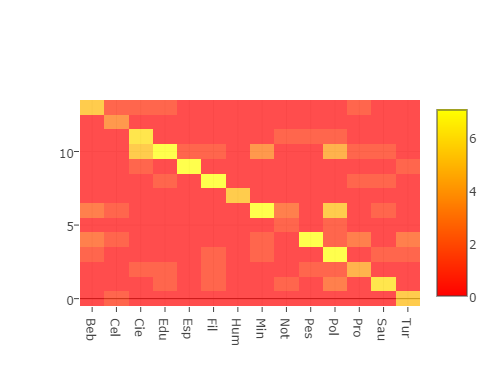
\includegraphics[width=0.9\textwidth]{weighted_nb_com_features_extras.png}
	\caption{Heatmap da matriz de confus�o da Tabela \ref{tab:weighted_nb_com_features_extras}}
	\label{fig:weighted_nb_com_features_extras}
\end{figure}

Outras estat�sticas analisadas s�o as precis�es, as abrang�ncias e os f1scores para cada uma das classes, conforme relacionado na Tabela \ref{tab:weighted_nb_com_features_extras_prec_rec}.

\begin{table}[tph]
	\begin{center}
		\begin{tabular}{ c  c  c  c }
			\hline
			Classe & Precisao & Abrangencia & F1score \\
			\hline
			Bebes & 0.555556 & 0.500000 & 0.526316 \\
			Celebridade & 1.000000 & 0.428571 & 0.600000 \\
			Ciencia & 0.666667 & 0.428571 & 0.521739 \\
			Educacao & 0.304348 & 0.636364 & 0.411765 \\
			Esporte & 0.777778 & 0.875000 & 0.823529 \\
			Filmes & 0.700000 & 0.636364 & 0.666667 \\
			Humor & 1.000000 & 1.000000 & 1.000000 \\
			Minorias & 0.560000 & 0.736842 & 0.636364 \\
			Noticias & 0.500000 & 0.200000 & 0.285714 \\
			Pessoal & 0.727273 & 0.923077 & 0.813559 \\
			Politica & 0.857143 & 0.666667 & 0.750000 \\
			Propaganda & 0.444444 & 0.444444 & 0.444444 \\
			Saude & 0.545455 & 0.600000 & 0.571429 \\
			Turismo & 0.833333 & 0.555556 & 0.666667 \\
			Media Micro & 0.656085 & 0.656085 & 0.656085 \\
			Media Macro & 0.676571 & 0.616533 & 0.645158 \\
			\hline
		\end{tabular}
	\end{center}
	\caption{Precis�o e abrangencia para Weighted NB com features extras}
	\label{tab:weighted_nb_com_features_extras_prec_rec}
\end{table}

\section{Utiliza��o dos links}
 
\section{Concatena��o do texto dos links}

\section{Fus�o de classes pequenas}

\section{Extens�o final desenvolvida}

\section{Teste de usabilidade}
% Usamos as heuristicas de Nielsen

\chapter{Conclus�es e Trabalhos Futuros}
\section{Conclus�es}

Este trabalho prop�s e analisou solu��es baseadas em Na�ve Bayes para se resolver o problema de classifica��o de postagens em redes sociais (especificamente no Facebook). Foram estudadas formas de se aliviar as considera��es de independ�ncia condicional, fazendo uso de pesos para as caracter�sticas.

Os resultados finais obtidos mostraram a viabilidade de se realizar este tipo de classifica��o, uma vez que foi poss�vel obter acur�cias superiores a 60\% (com F1score macro tamb�m superior a 60\%) utilizando-se uma base de dados relativamente pequena. Um aumento consider�vel na base de dados melhoraria muito a performance obtida.

Muitos dos erros cometidos pelo classificador final s�o justific�veis por terem ocorrido em postagens que na pr�tica poderiam pertencer a mais de uma classe. Deste modo, como trabalho futuro prop�e-se a realiza��o de um estudo semelhante com classificadores do tipo \emph{multi-class / multi-label}.

\section{Trabalhos Futuros}

\begin{itemize}
	\item \textbf{Aumentar a base de dados}\\
		Conforme os gr�ficos mostram, acredita-se que aumentando a base de dados os resultados melhorar�o. Para realizar isso pode-se executar o \emph{Crawler} mais vezes para obter mais dados e divulgar o plugin para mais pessoas e, assim, conseguir mais exemplos.
	\item \textbf{Utilizar \emph{Multi-class / Multi-label}}\\
		Muitos posts podem ser considerados como pertencendo a mais de uma categoria, o que indica que utilizando \emph{Multi-class / Multi-label} a qualidade do classificador possa aumentar significativamente.
	\item \textbf{Utilizar mais caracter�sticas da rede social}\\
		Foram utilizadas algumas caracter�sticas como autor do post, se � publicidade ou n�o, etc. Por�m ainda h� bastantes caracter�sticas que poderiam ser utilizadas, como, por exemplo, quem comentou em determinado post, o pr�prio texto dos coment�rios, entre outros.
		Um ponto interessante � que foi utilizado apenas o autor dos posts como caracter�stica, contudo, seria poss�vel aprofundar as informa��es sobre o autor de forma a capturar um pouco a estrutura da pr�pria rede social, como por exemplo quem s�o os amigos do autor, de quais grupos ele pertence, assim em diante.
	\item \textbf{Utilizar Informa��o M�tua para reconhecimento de novas classes}\\
		Outra sugest�o � utilizar o conceito de Informa��o M�tua para cria��o de novas classes sob o escopo do usu�rio. Se alguns dos posts do usu�rio fa�am com que a Informa��o M�tua entre duas classes seja grande isso talvez signifique que uma nova classe derivada seja melhor, como por exemplo os t�picos Sa�de e Engenharia para alguns posts pudessem ser substitu�dos por Bio-tecnologia.
		\item \textbf{Utilizar Informa��o M�tua para classes com poucos exemplos}\\
		Enquanto uma classe n�o atinja n�mero de exemplos significativo (que � obtido por meio do plugin sendo utilizado por "supervisores") pode-se utilizar a classe entre cuja Informa��o M�tua seja maior para efeitos de classifica��o de novos posts para n�o degradar a qualidade. Uma vez atingido um n�mero m�nimo de exemplos passa-se a utilizar a pr�pria classe.
\end{itemize}

% TODO: Tirar capitulos do Manga
\chapter{Instrumentos analisados}
\label{chap:instrumentos_analisados}
Todo programa de computador �, essencialmente, um algoritmo que transforma um sinal de entrada em um sinal de sa�da, portanto, entender os sinais de entrada � fundamental para o desenvolvimento e a depura��o de qualquer programa de computador.

No desenvolvimento deste trabalho diversos limites ter�o de ser impostos aos sinais sonoros de entrada. Ser�o estabelecidos limites, por exemplo � quantidade m�xima de notas tocadas por segundo, � nota mais grave e mais alta, � intensidade m�nima para um som ser considerado uma nota, etc. Entretanto, dada a multitude de instrumentos existente, � virtualmente imposs�vel estabelecer limites para os exemplos dados que satisfa�am aos sinais gerados por todos os instrumentos.

Assim, embora o escopo deste trabalho seja a transcri��o musical autom�tica de instrumentos monof�nicos temperados, independentemente da forma com que o som � gerado neles, as an�lises feitas a partir deste cap�tulo ser�o voltadas a um sub-conjunto espec�fico de instrumentos. Espera-se que este sub-conjunto seja representativo o bastante para que o algoritmo final desenvolvido seja tamb�m aplic�vel a diversos outros instrumentos. Este cap�tulo apresenta os instrumentos escolhidos e justifica as escolhas.

\section{Caracter�sticas de interesse}

Ao escolher os instrumentos, algumas caracter�sticas desejadas foram levantadas, essas s�o apresentadas a seguir:

\subsection{Mec�nismo de produ��o de som}

Deseja-se que os instrumentos analisados possuam mec�nismos de produ��o de som simples e para os quais j� existam modelos matem�ticos confi�veis. Isso tornar� poss�vel embasar as decis�es tomadas em modelos matem�ticos que representam o mundo real, e n�o apenas em suposi��es feitas com base em teoria musical.

\subsection{Timbre}

O timbre �, talvez, a caracter�stica mais marcante de um instrumento, e pode variar muito mesmo entre instrumentos de uma mesma fam�lia. Por esses motivos, deseja-se que os instrumentos analisados possuam timbres consideravelmente distintos. Isso ajudar� a elaborar algoritmos que funcionem em uma gama diversa de instrumentos.

\subsection{Tom}

Em um �nico instrumento, uma mesma nota pode ser tocada de diversas formas, ou tons, dependendo da sensa��o que o m�sico deseja transmitir. Por exemplo, uma nota pode ser suave ou agressiva; viva ou fria. � interessante que os instrumentos escolhidos sejam capazes de gerar uma vasta gama de tons, tamb�m para que os algoritmos elaborados sejam pouco espec�ficos aos instrumentos escolhidos.

\subsection{Popularidade}

Para que os algoritmos desenvolvidos possuam aplica��es reais, � interessante que eles funcionem bem para instrumentos populares, portanto faz sentido escolher instrumentos que sejam conhecidos e bastante utilizados.

\section{Instrumentos escolhidos}

Com base nas caracter�sticas levantadas, a classe dos instrumentos de sopro foi escolhida. Al�m de populares, a produ��o de som por esses instrumentos j� � um processo bem conhecido e que pode ser aproximado por modelos majoritariamente lineares \cite{fletcher_1979}. Estes instrumentos tamb�m possuem timbres bastante caracter�sticos e distintos uns dos outros. Ainda, instrumentos como a flauta transversal permitem ao instrumentista realizar uma vasta gama de tonalidades dependendo de sua enbocadura, controle de respira��o, etc.

Dentro da classe dos instrumentos de sopro, os seguintes instrumentos foram selecionados:

\begin{enumerate}
    \item Flauta doce
    \item \textit{Tin whistle}
    \item P�fano
    \item Flauta transversal ocidental
    \item Flauta transversal chinesa (\textit{dizi})
    \item Ocarina
\end{enumerate}

Cada instrumento ser� apresentado partindo de uma breve descri��o hist�rica, seguida de caracter�sticas de interesse para o trabalho e de uma an�lise espectral de algumas notas tocadas no instrumento. Nota-se que o espectro gerado por cada instrumento pode variar de acordo com a habilidade do instrumentista e com as t�cnicas que ele deseja executar \cite{fletcher_1975}. Entretanto, consideramos que essas varia��es s�o desprez�veis quando comparadas �s causadas pelo uso de instrumentos diferentes e, portanto, podem ser desconsideradas nesse cap�tulo, cujo prop�sito � apenas comparar o espectro de diferentes instrumentos e discutir os resultados esperados para cada um.

\section{Flauta doce}

A flauta doce � um instrumento de origem medieval, sua popularidade em apresenta��es diminuiu consideravelmente com o surgimento de instrumentos voltados para orquestras. Hoje, por ser um instrumento relativamente simples e f�cil de se tocar, a flauta doce � amplamente utilizada no ensino de m�sica.

Neste trabalho, ser� utilizada uma flauta doce soprano germ�nica afinada em d� maior (modelo Yamaha YRS-23Y). Este modelo possui oito buracos, � feito de pl�stico e � amplamente utilizado por iniciantes. O termo "soprano" remete ao fato da nota mais grave produzida por esta flauta ser um C5, enquanto o termo "germ�nica" remete � forma com que os buracos na flauta devem ser utilizados para produzir notas espec�ficas.

\subsection{Caracter�sticas}

A flauta doce utilizada � capaz de produzir 3 oitavas crom�ticas\footnote{A maioria dos instrumentos de sopro n�o possui um limite superior para as notas produzidas \cite{fletcher_1979}. Os limites apresentados aqui s�o os dados pelo fabricante do modelo utilizado, e refletem o que � pedido no repert�rio cl�ssico.} a partir do C5.

Uma caracter�stica que facilitar� este trabalho � que a estrutura geom�trica da flauta doce � totalmente controlada pelo fabricante \cite{auvray_2014}. Seu bocal � feito de forma a direcionar o jato de ar produzido pelo flautista contra uma superf�cie afiada. Com isso, o flautista n�o precisa se preocupar em direcionar o jato de ar gerado, e tem que apenas controlar a press�o exercida. O bocal da flauta doce tamb�m � projetado para facilitar o controle da press�o exercida e, como resultado, o flautista � capaz de produzir duas oitavas com modifica��es m�nimas no jato de ar que produz, e sem ter de modificar sua geometria. Isso tamb�m significa que a tonalidade da flauta doce varia pouco, embora fatores como resson�ncia na cavidade oral do instrumentista ainda permitam a ele leves modifica��es no tom \cite{auvray_2014}.

Por outro lado, a flauta doce n�o possui nenhum mecanismo para ajudar o flautista a pressionar os buracos em seu corpo. Assim, embora seja relativamente f�cil produzir e alternar entre as notas da escala de d� maior, produzir uma escala crom�tica � uma tarefa dif�cil que requer muito controle do posicionamento dos dedos, sendo necess�rio encobrir certos buracos levemente, com um alto grau de precis�o. Ainda, pode ser necess�rio alternar muitos dedos entre notas crom�ticas, o que facilmente produz estados transientes desagrad�veis em frases tocadas em \textit{legato}.

\subsection{An�lise espectral}

\begin{figure}[ht!]
    \centering	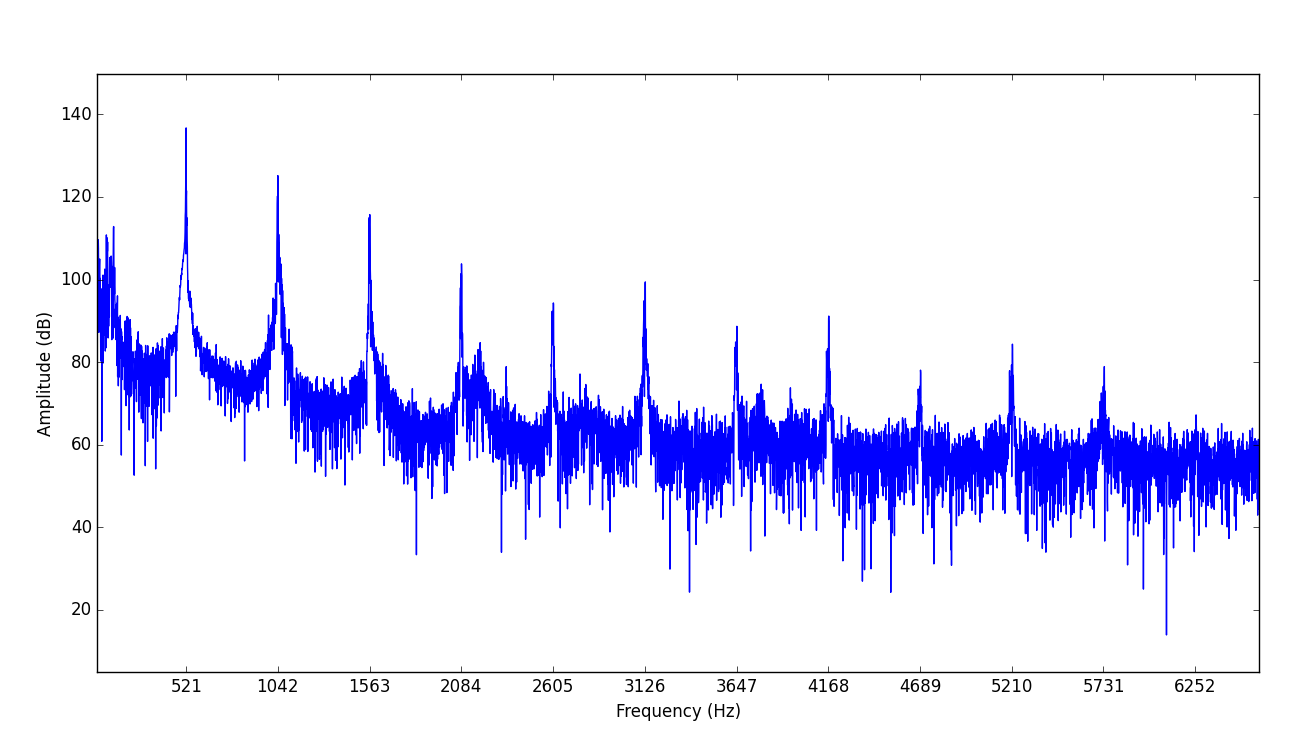
\includegraphics[width=1.0\textwidth]{FlautaDoce-C5.png}
    \caption{Espectro para a nota C5 tocada em uma flauta doce Yamaha YRS-23Y obtido a partir da FFT em 1 segundo de grava��o.}
    \label{fig:FlautaDoce-C5}
\end{figure}

A figura \ref{fig:FlautaDoce-C5} mostra o espectro obtido em 1 segundo de grava��o da nota mais grave produzida pela flauta doce (C5). Observa-se que na flauta doce o componente fundamental � o mais acentuado, sendo seguido por quatro harm�nicos cuja amplitude decai em cerca de $10 \textnormal{dB}/\textnormal{harm�nico}$. A partir do quinto harm�nico o comportamento deixa de seguir um padr�o simples. Ainda, o m�ximo em $521 Hz$ indica que a flauta doce utilizada est� afinada com o A4 em cerca de $438 	Hz$, o que sugere a afina��o padr�o de $440 Hz$ com uma pequena margem de erro que pode ter sido causada, por exemplo, por diferen�as de temperatura. Por fim, � interessante observar que os harm�nicos da flauta doce seguem a s�rie:

\begin{equation}
H_n = H_0(n+1)
\end{equation}

Sendo $H_0$ o harm�nico fundamental. Outros instrumentos podem seguir a s�rie:

\begin{equation}
H_n = H_0(2n+1)
\end{equation}

Uma explica��o f�sica para os instrumentos de sopro gerarem uma s�rie ou a outra pode ser encontrada em \cite{fletcher_1979}.

\begin{figure}[ht!]
    \centering	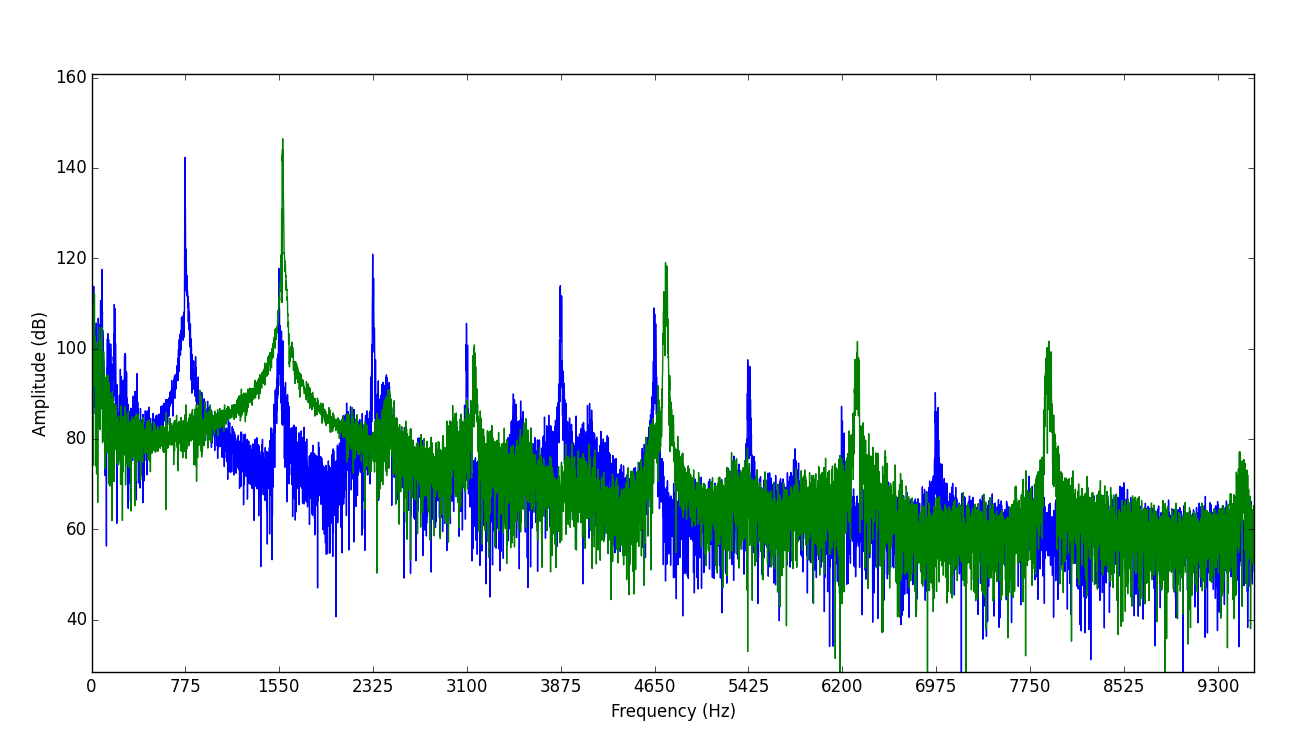
\includegraphics[width=1.0\textwidth]{FlautaDoce-G5G6.png}
    \caption{Espectro para um G5 (azul) e um G6 (verde) tocados em uma flauta doce Yamaha YRS-23Y obtido a partir da FFT em 1 segundo de grava��o.}
    \label{fig:FlautaDoce-G5G6}
\end{figure}

J� a figura \ref{fig:FlautaDoce-G5G6} compara o espectro de um G5 e de um G6 uma oitava acima. � interessante observar que a amplitude relativa entre os harm�nicos � bastante diferente da amplitude relativa para a nota C5 da figura \ref{fig:FlautaDoce-C5}, sendo o segundo harm�nico mais intenso que o primeiro. Apesar disso, tanto o G5 quanto o G6 possuem amplitudes relativas semelhantes entre si. Outro fator interessante � que os harm�nicos produzidos n�o s�o posicionados exatamente nas mesmas frequ�ncias.

Por fim, observamos que a nota G6 tem uma leve tend�ncia de gerar componentes posicionados nos harm�nicos de um G5 que n�o s�o seus pr�prios harm�nicos. Isso pode ser visto na frequ�ncia de ($2325 Hz$), que � um m�ltiplo da frequ�ncia fundamental do G5 $775 Hz$, mas n�o � um m�ltiplo do G6 ($1550 Hz$). Isto dificultar� a distin��o dessas duas notas no algoritmo de detec��o de frequ�ncia fundamental.

\subsection{Conclus�es}

Espera-se que o programa desenvolvido nesse trabalho seja capaz de identificar muito bem m�sicas em d� maior tocadas nessa flauta, mas que encontre dificuldades em m�sicas crom�ticas, especialmente se houver muitas frases em \textit{legato}. Espera-se que essa dificuldade seja mais relacionada � erros cometidos pelo instrumentista do que de erros do algoritmo.

\section{\textit{Tin Whistle}}

O \textit{tin whistle} � um instrumento de sopro popular na m�sica celta, seu corpo costuma ser feito de estanho, da� o nome. A m�sica popular celta � conhecida por ritmos r�pidos e frases com muitos ornamentos, e isso se reflete nas caracter�sticas do \textit{whistle}.

Nesse trabalho ser� utilizado um \textit{whistle} Clarke SBDC afinado em R� maior, que possui 6 buracos.

\subsection{Caracter�sticas}

O \textit{whistle} utilizado � capaz de produzir 2 oitavas nas escalas de R� maior ou Sol maior, a partir de um D5.

O \textit{whistle} � bastante semelhante � flauta doce, mas � um instrumento de confec��o mais simples e seu bocal ajuda muito menos o instrumentista a controlar o jato de ar, sendo mais f�cil gerar notas desafinadas ou desagrad�veis. Por outro lado, os buracos no corpo do \textit{whistle} s�o mais simples, e � muito f�cil transitar entre as notas na escala para a qual ele foi afinado. Isso permite ao instrumentista tocar passagens muito r�pidas e com diversos ornamentos sem gerar muitos transientes desagrad�veis.

\subsection{An�lise espectral}

\begin{figure}[ht!]
    \centering	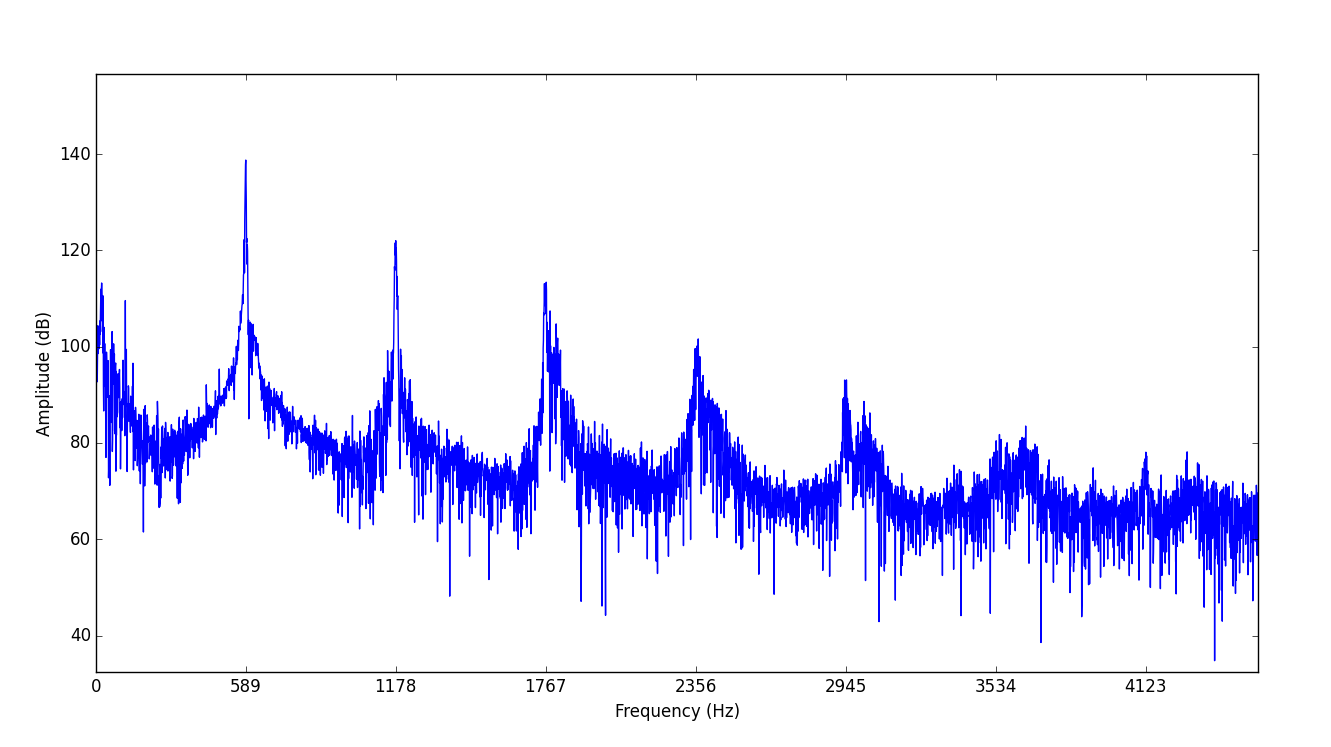
\includegraphics[width=1.0\textwidth]{TinWhistle-D5.png}
    \caption{Espectro para a nota D5 tocada em um \textit{whistle} Clarke SBDC obtido a partir da FFT em 1 segundo de grava��o.}
    \label{fig:TinWhistle-D5}
\end{figure}

Na figura \ref{fig:TinWhistle-D5} podemos ver que, relativamente � flauta doce, o \textit{whistle} gera menos harm�nicos significativos. Al�m disso, os picos nas frequ�ncias dos harm�nicos "vazam" mais para as frequ�ncias vizinhas. Isso pode ser atribu�do ao bocal mais primitivo do \text{whistle}, que direciona menos o jato de ar produzido pelo instrumentista, fazendo com que parte da energia do jato seja desperdi�ada e gere componentes indesejados.

\begin{figure}[ht!]
    \centering	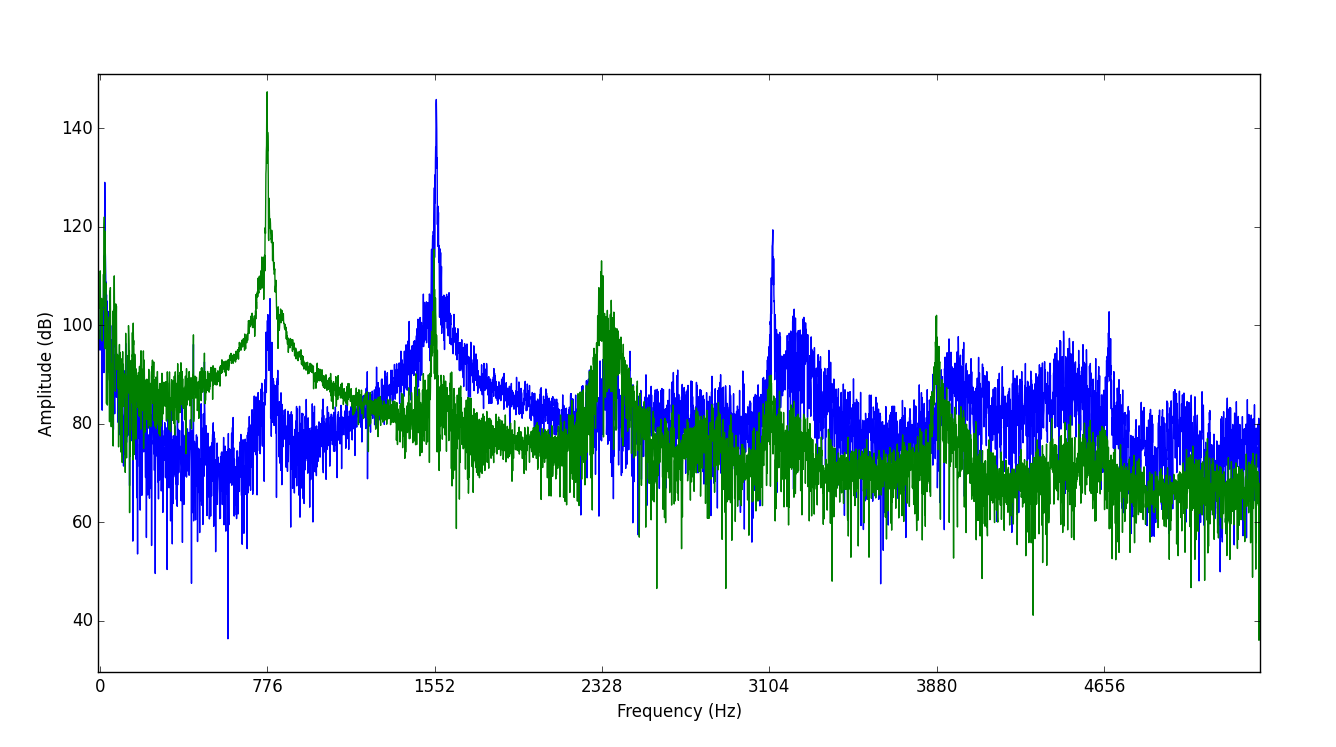
\includegraphics[width=1.0\textwidth]{TinWhistle-G5G6.png}
    \caption{Espectro para um G5 (verde) e um G6 (azul) tocados em um \textit{whistle} Clarke SBDC obtido a partir da FFT em 1 segundo de grava��o.}
    \label{fig:TinWhistle-G5G6}
\end{figure}

Na figura \ref{fig:TinWhistle-G5G6} podemos comparar a nota G6 com a nota G5 no \textit{whistle}. � interessante observar que na nota G6 os ru�dos s�o muito mais intensos do que na G5, lembramos que no \textit{whistle} � necess�rio aumentar consideravelmente a intensidade do jato de ar para trocar entre oitavas, como o bocal do whistle n�o faz nenhum ajuste no jato de ar, a maior intensidade causa um desperd�cio maior de energia, que se reflete no r�ido.

Adicionalmente, nota-se que a nota G6 gera um componente harm�nico na frequ�ncia fundamental da nota G5, mas com amplitude reduzida. Isso � esperado pois as duas notas possuem o mesmo dedilhado e, portanto, a forma geom�trica do instrumento permite que esse componente seja formado. Esse datalhe pode causar erros na classifica��o correta da oitava de uma nota tocada.

\subsection{Conclus�es}

Relativamente a flauta doce, espera-se que nos sinais provenientes do \textit{whistle} seja mais f�cil identificar passagens r�pidas e com ornamentos, mas que para m�sicas lentas a precis�o seja menor, devido a maior dificuldade em se controlar o jato de ar. Ainda, espera-se uma dificuldade adicional nas notas mais agudas, que possuem mais ru�do e componentes nas mesmas frequ�ncias das notas correspondentes na oitava inferior.

\section{P�fano}

O p�fano � uma flauta transversal pequena com timbre estridente. � um instrumento bastante simples, sendo desprovido de um bocal e, portanto, delegando o controle do jato de ar totalmente ao instrumentista.

Nesse trabalho ser� utilizado um p�fano Yamaha YRF-21 afinado em D� maior, que � feito de pl�stico e possui 9 buracos em seu corpo, sendo um destinado ao sopro.

\subsection{Caracter�sticas}

O p�fano utilizado � capaz de produzir cromaticamente as notas entre C5 e E7.

O p�fano escolhido � bastante semelhante � flauta doce, tanto em material quanto na posi��o dos dedilhados. A maior diferen�a � o fato do p�fano ser desprovido de um bocal e de ser empunhado transversalmente. A aus�ncia de um bocal permite ao instrumentista controlar sua embocadura de forma a variar muito o tom do instrumento. Assim, as dificuldades apresentadas para a flauta doce se mant�m, sendo acrescentadas dificuldades em identificar precisamente as notas, que podem sofrer muitas varia��es de tom.

Nota-se, em especial, que a transi��o entre oitavas no p�fano � muito mais dif�cil de se realizar do que nos instrumentos apresentados anteriormente. Tanto na flauta doce quando no \textit{whistle} essa transi��o pode ser feita usando um dedilhado levemente diferente e acelerando um pouco o jato de ar. Entretanto, como o p�fano n�o possui um bocal para direcionar o jato de ar, o instrumentista precisa alterar consideravelmente a sua embocadura de forma a gerar um jato mais r�pido que continua atingindo a superf�cie do instrumento no �ngulo correto e com a largura adequada. Esse aspecto ser� analisado espectralmente a seguir.

\subsection{An�lise espectral}

\begin{figure}[ht!]
    \centering	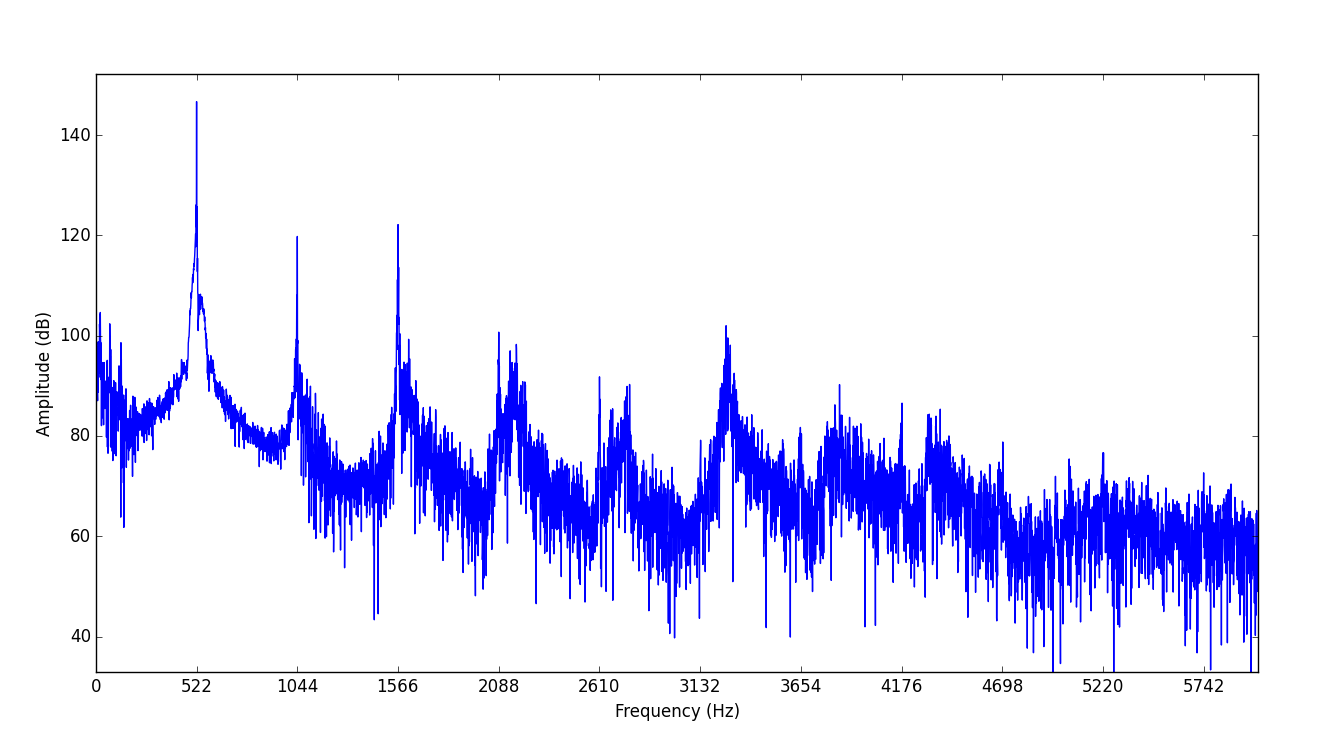
\includegraphics[width=1.0\textwidth]{Fife-C5.png}
    \caption{Espectro para a nota C5 tocada em um p�fano Yamaha YRF-21 obtido a partir da FFT em 1 segundo de grava��o.}
    \label{fig:Fife-C5}
\end{figure}

Na figura \ref{fig:Fife-C5} temos o espectro para um C5, a nota mais grave atingida pelo p�fano. � poss�vel reconhecer cerca de $8$ harm�nicos, sendo os $3$ primeiros bem mais significativos. Ainda, nota-se que os harm�nicos a partir do terceiro s�o acompanhados de amplitudes consider�veis em suas redondezas, de forma semelhante ao que ocorre no \textit{whistle}, e contr�ria � flauta doce.

\subsection{Conclus�es}

Relativamente a flauta doce, espera-se que nos sinais provenientes do p�fano seja mais dif�cil identificar precisamente a frequ�ncia fundamental das notas, e que ocorram erros relativos � oitava da nota tocada. Esses problemas se reduzem de acordo com a habilidade do instrumentista.

\section{Flauta transversal ocidental}

A flauta transversal ocidental � um dos instrumentos de sopro mais populares em orquestras. Foi feito a partir da modifica��o de flautas transversais medievais (semelhantes ao p�fano). As principais melhorias introduzidas foram um corpo de metal, que � capaz de gerar notas muito mais altas e que podem ser carregadas sobre os demais instrumentos de uma orquestra, e um mecanismo de bot�es e molas que deixa os dedilhados muito mais confort�veis, pois os bot�es podem ser projetados para ocuparem posi��es confort�veis sem prejudizar a afina��o do instrumento, al�m de facilitarem a tarefa de encobrir  totalmente os buracos.

Nesse trabalho ser� utilizada uma flauta transversal afinada em D� maior, modelo Hallelu HFL-200.

\subsection{Caracter�sticas}

A flauta transversal utilizada � capaz de produzir cromaticamente tr�s oitavas a partir do C4.

Em rela��o aos instrumentos apresentados anteriormente, nota-se que a flauta transversal escolhida � capaz de produzir notas mais graves. Analisar essas notas ser� uma tarefa mais dif�cil, primeiro porque a diferen�a absoluta da frequ�ncia entre duas notas separadas por um semitom ser� menor e, segundo, porque a frequ�ncia menor aumenta o tempo em que o instrumento se encontra em estados transit�rios \cite{fletcher_1979}.

Em rela��o � flauta doce e ao \textit{whistle}, a aus�ncia de um bocal dificulta a identifica��o das notas tocadas, pois h� uma variedade muito maior de tons que podem ser produzidos, assim como no p�fano. Por outro lado, a constru��o mais cuidadosa do instrumento e os bot�es mec�nicos ajudar�o a produzir tons mais limpos do que no p�fano, e facilitar�o a identifica��o de notas em passagens r�pidas e com \textit{legatos}.

\subsection{An�lise espectral}

\begin{figure}[ht!]
    \centering	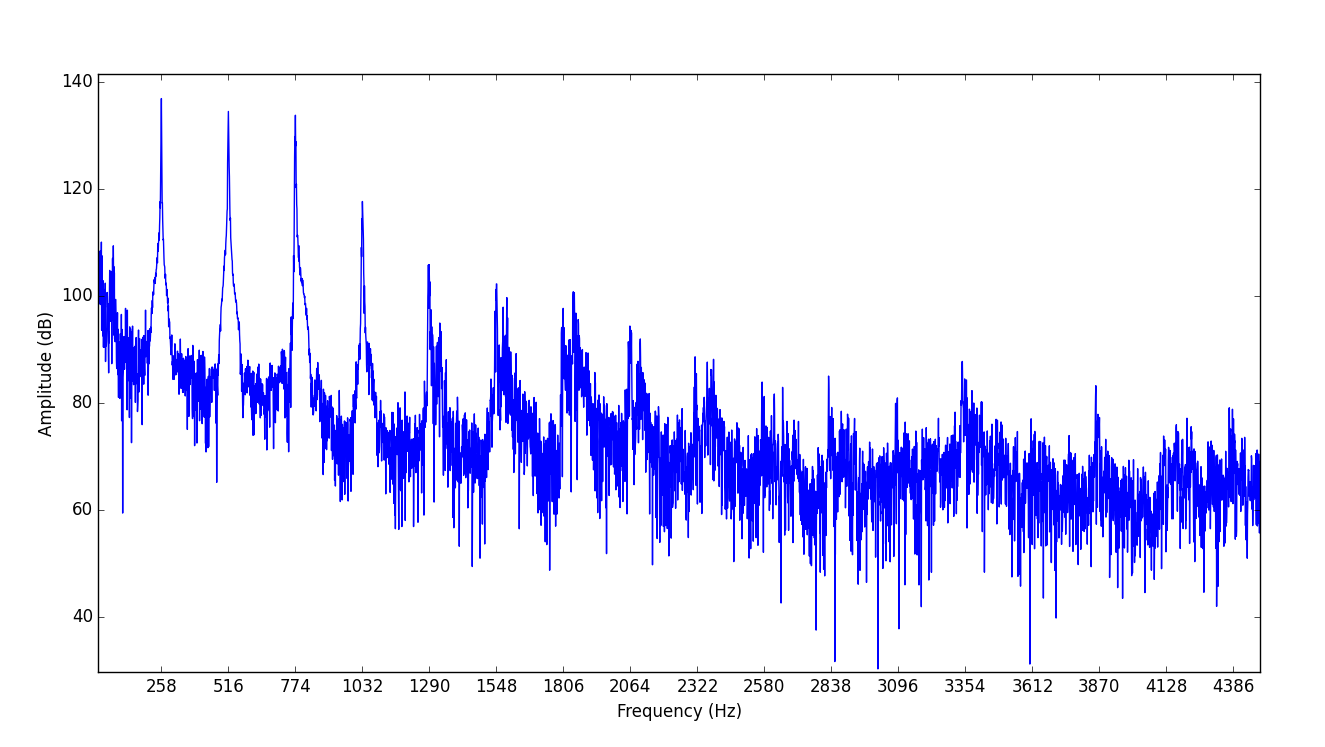
\includegraphics[width=1.0\textwidth]{FlautaTransversal-C4.png}
    \caption{Espectro para a nota C4 tocada em uma flauta transversal Hallelu HFL-200 obtido a partir da FFT em 1 segundo de grava��o.}
    \label{fig:FlautaTransversal-C4}
\end{figure}

\begin{figure}[ht!]
    \centering	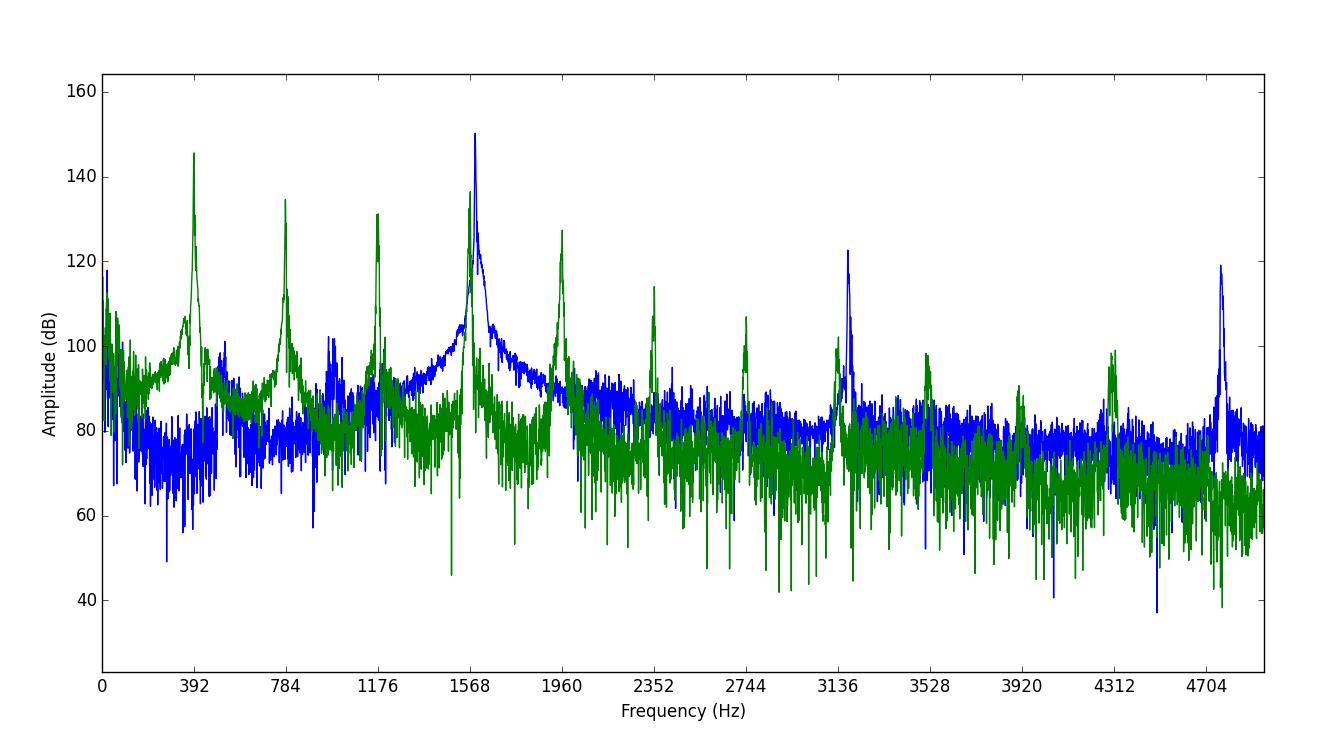
\includegraphics[width=1.0\textwidth]{FlautaTransversal-G4G6.png}
    \caption{Espectro para um G4 (verde) e um G6 (azul) tocados em uma flauta transversal Hallelu HFL-200C obtido a partir da FFT em 1 segundo de grava��o.}
    \label{fig:FlautaTransversal-G4G6}
\end{figure}

Na figura \ref{fig:FlautaTransversal-C4} vemos o espectro para um C4, a nota mais grave produz�vel na flauta transversal. J� na figura \ref{fig:FlautaTransversal-G4G6} vemos as notas G4 e G6 na mesma flauta.

Primeiramente, observamos que na nota C4 os tr�s primeiros harm�nicos possuem amplitude bastante pr�xima. A nota C4 na flauta transversal � relativamente dif�cil de ser tocada, sendo necess�rio um controle bastante preciso do jato de ar produzido. Pequenos erros no jato podem transformar a nota em um C5, o que justifica a amplitude relativamente alta do segundo harm�nico (que seria o fundamental para um C5). Al�m disso, os harm�nicos mais altos n�o possuem picos t�o bem definidos quanto os mais baixos, o que indica um som menos limpo do que o da flauta doce, por exemplo.

Comparando a figura \ref{fig:FlautaTransversal-C4} com a \ref{fig:FlautaTransversal-G4G6}, podemos ver que a nota G4, apesar de estar na mesma oitava que a C4, n�o apresenta as dificuldades apresentadas anteriormente, possuindo um espectro parecido com os produzidos pela flauta doce, em que cada harm�nico possui um pico bem definido no espectro.

Por fim, vemos que a nota G6, mesmo estando duas oitavas acima da nota G4, n�o apresenta um ru�do significativamente maior e nem gera componentes sub-harm�nicos significativos (dificuldades presentes, por exemplo, nas notas altas do \textit{whistle}). Nota-se que a flauta transversal � um instrumento feito para ser ouvido sob uma orquestra e �, portanto, mais potente. A energia perdida no jato de ar produzido pelo flautista � menos significativa. Al�m disso, a aus�ncia de um bocal permite ao flautista ajustar livremente a embocadura, de forma a aproveitar bem a energia do jato de ar e controlar os componentes sub-harm�nicos.

\subsection{Conclus�es}

Espera-se que a identifica��o das notas na flauta transversal seja mais f�cil que nos demais instrumentos a partir da segunda oitava (C5-C7), desde que o flautista seja h�bil o bastante para controlar sua embocadura corretamente. Na oitava inferior (C4-B4) podem haver mais erros devido � estados transientes e � maior proximidade entre as frequ�ncias fundamentais. Por fim, espera-se ser mais f�cil identificar passagens crom�ticas na flauta transversal do que nos outros instrumentos, devido aos bot�es mec�nicos que facilitam os dedilhados para notas acidentais.

\section{Flauta transversal chinesa (\textit{dizi})}

O \textit{dizi}, comumente conhecido como flauta transversal chinesa, � um instrumento popular na china, sendo utilizado tanto em m�sica popular quanto em �peras e orquestras chinesas. Costuma ser feito artesanalmente a partir de uma �nica pe�a de bambu, que � furada nas posi��es desejadas para os dedilhados.

Nesse trabalho ser� utilizado um \textit{dizi} artesanal de baixa qualidade importado da china.

\subsection{Caracter�sticas}

O \textit{dizi} utilizado � capaz de produzir um subconjunto espec�fico de notas entre E5 e B7. Seu temperamento n�o gera notas separadas por semitons, o que dificultar� muito a tarefa de classific�-las.

Em rela��o ao p�fano, a produ��o artesanal do \textit{dizi} faz com que as notas produzidas possuam v�rias imperfei��es, tanto na afina��o, pela posi��o dos buracos, quanto no tom, pela maior dificuldade em se encobrir totalmente os buracos. Ainda, o \textit{dizi} escolhido possui 11 buracos em seu corpo, e seus dedilhados s�o pouco confort�veis, sendo dif�cil tocar passagens r�pidas com precis�o

Por n�o ser muito adequado � m�sica ocidental, ele ser� utilizado brevemente para testar os tons produzidos por instrumentos pouco comuns na m�sica ocidental, e com afina��es ex�ticas.

\subsection{An�lise espectral}

\subsection{Conclus�es}

Espera-se que a identifica��o correta das notas tocadas no \textit{dizi} seja bastante dif�cil e que seja feita com sucesso apenas para m�sicas mais lentas, a menos que o instrumentista seja muito habilidoso. Ainda, espera-se que seja dif�cil obter as notas exatas devido � afina��o n�o temperada do \textit{dizi}.
    
\section{Ocarina}

A ocarina � um instrumento de sopro globular geralmente feito de cer�mica. � um dos instrumentos mais antigos conhecidos, e pode ter diversas formas.

Nesse trabalho ser� utilizada uma ocarina modelo "TOTMC Legend of Zelda Ocarina of Time Triforce Link TOLO248" de 12 buracos afinada em D� maior.

\subsection{Caracter�sticas}

A ocarina escolhida � capaz de produzir cromaticamente as notas no intervalo A4-F6.

O corpo globular da ocarina dificulta a cria��o de harm�nicos, sendo a frequ�ncia fundamental muito mais intensa do que as mais altas. Entretanto, espera-se que a manufatura em cer�mica apresente mais imperfei��es do que os instrumentos em pl�stico e metal, o que pode ser constadado, por exemplo, no formato irregular dos buracos. Tamb�m nota-se que os dedilhados na ocarina s�o pouco confort�veis, sendo muito f�cil n�o encobrir corretamente alguns dos buracos.

\subsection{An�lise espectral}

\begin{figure}[ht!]
    \centering	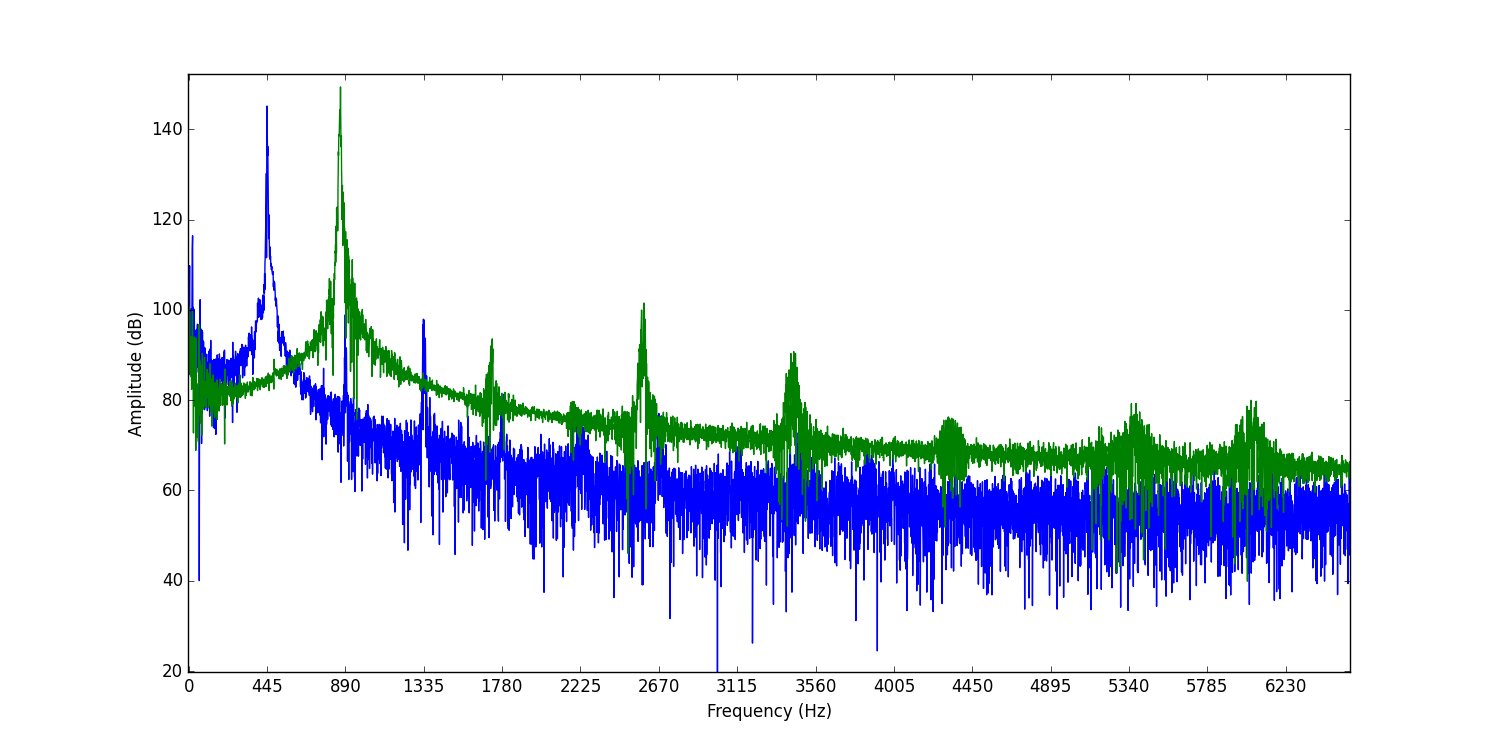
\includegraphics[width=1.0\textwidth]{Ocarina-A4A5.png}
    \caption{Espectro para um A4 (azul) e um A5 (verde) tocados na ocarina escolhida, obtido a partir da FFT em 1 segundo de grava��o.}
    \label{fig:Ocarina-A4A5}
\end{figure}

Na figura \ref{fig:Ocarina-A4A5} comprovamos que apenas o harm�nico fundamental � significativo na ocarina.

\subsection{Conclus�es}

Como na ocarina apenas a frequ�ncia fundamental � consider�vel, espera-se que as notas identificadas estejam na oitava correta. Entretanto, pode haver erros na identifica��o de notas separadas por semitons, pois a decis�o ter� de ser tomada com a informa��o de um �nico harm�nico.

\chapter{Algoritmos de Otimiza��o}
\section{Algoritmo Gen�tico}

Algoritmos Gen�ticos (\acs{AG}s) s�o inspirados na Teoria da Evolu��o de Darwin \cite{holland_1975}. Nestas t�cnicas,  mant�m-se uma popula��o de solu��es candidatas, chamadas cromossomos, que ``evoluem'' guiadas por uma medida de qualidade (fun��o de \emph{fitness}) atrav�s da aplica��o de opera��es inspiradas pela evolu��o natural: sele��o, muta��o, \textit{crossover} e sobreviv�ncia dos mais aptos. Inicialmente, a popula��o � composta por \(S_i\) (par�metro do AG) cromossomos gerados aleatoriamente.

Existem diversas variantes de \ac{AG}. A seguir, explica-se os detalhes de \ac{AG} nas formas que s�o utilizadas com mais frequ�ncia. No final, apresenta-se tamb�m um pseudoc�digo para \ac{AG}. Uma descri��o mais geral de \ac{AG} pode ser encontrada em \cite{norvig}.

\subsection*{Cromossomo}

Um cromossomo � um candidato � solu��o �tima. Cada parte do cromossomo � chamada gene. A boa codifica��o do problema em cromossomo � um fator fundamental para o sucesso do algoritmo. No caso do problema de otimizar um conjunto de par�metros, a codifica��o em cromossomo �bvia � representar uma dada inst�ncia por um vetor, em que cada posi��o (gene) corresponde a um par�metro espec�fico.

\subsection*{Fun��o de \textit{Fitness}}

� uma fun��o que, dado um cromossomo, retorna um n�mero real (\textit{fitness}) que mede o qu�o bom � este cromossomo para resolver o problema. Em geral, assume-se a conven��o que quanto maior o \textit{fitness}, melhor o cromossomo.

\subsection*{Sele��o}

A cada gera��o uma parte da popula��o � escolhida para reprodu��o. Nesse processo, a probabilidade de um cromossomo ser escolhido � geralmente proporcional ao seu \textit{fitness} (sele��o por roleta). Outras formas de selecionar os que ir�o se reproduzir tamb�m s�o aplicadas. O n�mero de quantos indiv�duos \(R\) (par�metro do \ac{AG}) s�o escolhidos para reprodu��o a cada gera��o � um par�metro do \ac{AG}.

\subsection*{Muta��o}

Corresponde ao fator de caminhada aleat�ria do algoritmo. Dado um cromossomo, essa opera��o itera sobre cada gene e o troca por um valor aleat�rio (dentro do dom�nio do gene) com uma certa probabilidade de muta��o \(p_m\) (par�metro do \ac{AG}).

\subsection*{\textit{Crossover}}

Dados dois cromossomos escolhidos para se reproduzir, � interessante (assim como ocorre na Natureza) que, ao inv�s de se ter filhos como c�pia id�ntica dos pais, fa�a-se uma recombina��o dos genes dos pais de modo a produzir cromossomos com caracter�sticas mistas. Assim, o \textit{crossover} em um \ac{AG} segue um procedimento an�logo ao \textit{crossover} biol�gico: escolhe-se um ponto de quebra e cria-se um cromossomo filho tomando-se a parte do primeiro pai antes do ponto de quebra e a do segundo ap�s esse ponto. Observe que esse processo pode ser generalizado para m�ltiplos pontos de quebra, embora comumente se utilize um �nico ponto.

\subsection*{Sobreviv�ncia dos Mais Aptos}

Como a cada itera��o ocorre reprodu��o, a popula��o tende a aumentar indefinidamente. Para evitar isso, assume-se um tamanho de popula��o m�ximo \(S_m\) (par�metro do \ac{AG}) e elimina-se os menos aptos (com menores valores de \textit{fitness}) a cada gera��o. Outra forma de realizar esta opera��o envolve escolher probabilisticamente os sobreviventes com probabilidade de escolha dependente do valor de \emph{fitness}.

\newpage

\begin{algorithm}[H]
\Begin{
$Populacao\gets PopulacaoAleatoria(S_i)$\;
$Fitnesses\gets CalcularFitnesses(Populacao)$\;
\While{crit�rio de parada n�o satisfeito}{
$Pais\gets Selecao(Populacao, Fitnesses, R)$\;
$Filhos\gets Crossover(Pais)$\;
$Populacao\gets Populacao\cup Filhos$\;
$Populacao\gets Mutacao(Populacao, p_m)$\;
$Fitnesses\gets CalcularFitnesses(Populacao)$\;
$Populacao\gets MaisAptos(Populacao, Fitnesses, S_m)$\;
}
}
\caption{Pseudoc�digo do Algoritmo Gen�tico.}
\label{alg:ag}
\end{algorithm}

\section{Particle Swarm Optimization}
\label{sec:pso}

\ac{PSO} � um algoritmo de otimiza��o iterativo que busca uma candidata � solu��o �tima conforme uma medida de qualidade. O algoritmo trabalha com um espa�o de busca em \(D\) dimens�es limitado inferiormente por \(\boldsymbol{l}\) e superiormente por \(\boldsymbol{u}\). Inicialmente, sorteia-se \(P\) ``part�culas'' aleatoriamente tal que a posi��o \(\boldsymbol{x_i}\) e a velocidade \(\boldsymbol{v_i}\) de cada part�cula \(p_i\) satisfazem as equa��es \ref{eq:posicao_pso} e \ref{eq:velocidade_pso}, respectivamente.

\begin{equation}
\boldsymbol{x_i}(d)\in [\boldsymbol{l}(d), \boldsymbol{u}(d)], d=1,\ldots ,D
\label{eq:posicao_pso}
\end{equation}

\begin{equation}
\boldsymbol{v_i}(d)\in [-|\boldsymbol{u}(d)-\boldsymbol{l}(d)|, |\boldsymbol{u}(d)-\boldsymbol{l}(d)|], d=1,\ldots ,D
\label{eq:velocidade_pso}
\end{equation}

Assim, a cada itera��o, cada posi��o de part�cula � avaliada pela fun��o de medida de qualidade \(f:\mathbb{R}^{D}\rightarrow\mathbb{R}\) e atualiza-se \(\boldsymbol{b_i}\), a melhor posi��o da part�cula \(p_i\) at� ent�o,  e \(\boldsymbol{g}\), a melhor posi��o global de part�cula at� o momento, segundo \(f\). A partir deste ponto, assume-se que o objetivo � maximizar \(f(\boldsymbol{x})\). Note que isso n�o � limita��o, pois se o objetivo � minimizar \(f(\boldsymbol{x})\), basta executar o algoritmo com \(g(\boldsymbol{x})=-f(\boldsymbol{x})\). Por fim, atualiza-se a velocidade e a posi��o de cada part�cula segundo as equa��es  \ref{eq:atualiza_velocidade_pso} e \ref{eq:atualiza_posicao_pso}, respectivamente.

\begin{equation}
\boldsymbol{v_i}\gets \omega \boldsymbol{v_i} + \varphi_p r_p (\boldsymbol{b_i} - \boldsymbol{x_i}) + \varphi_g r_g (\boldsymbol{g} - \boldsymbol{x_i})
\label{eq:atualiza_velocidade_pso}
\end{equation}

\begin{equation}
\boldsymbol{x_i}\gets \boldsymbol{x_i} + \boldsymbol{v_i}
\label{eq:atualiza_posicao_pso}
\end{equation}

Em que \(\omega\), \(\varphi_p\) e \(\varphi_g\) s�o par�metros do algoritmo, e \(r_p\) e \(r_g\) s�o n�mero reais aleat�rios entre 0 e 1. O m�todo prossegue at� que algum crit�rio de parada seja atingido (n�mero m�ximo de itera��es, tempo m�ximo, limite de processamento, etc.). Um pseudoc�digo para \ac{PSO} � apresentado no Algoritmo \ref{alg:pso}.

O \ac{PSO} tem vantagens por n�o impor requisitos sobre o problema a ser otimizado al�m do conhecimento do espa�o de busca e de uma medida de desempenho. Entretanto, seu comportamento n�o � bem compreendido e n�o h� garantia de converg�ncia para solu��o �tima. Al�m disso, o m�todo sofre de tend�ncia a convergir para m�ximos locais.

\newpage

\begin{algorithm}[H]
\Begin{
\For{$i\gets 1,\ldots,P$} {
	\For{$d\gets 1,\ldots,D$}{
		$\boldsymbol{x_i}(d)\gets random(\boldsymbol{l}(d), \boldsymbol{u}(d))$\;
		$\Delta\gets |\boldsymbol{u}(d)-\boldsymbol{l}(d)|$\;
		$\boldsymbol{v_i}(d)\gets random(-\Delta,\Delta)$\;
	}
	$\boldsymbol{b_i}\gets \boldsymbol{x_i}$\;
	\If{$f(\boldsymbol{b_i}) > f(\boldsymbol{g})$}{
		$\boldsymbol{g}\gets \boldsymbol{b_i}$\;
	}
}

\While{crit�rio de parada n�o satisfeito}{
	\For{$i\gets 1,\ldots,P$}{
		\For{$d\gets 1,\ldots,D$}{
			$r_p\gets random(0,1)$\;
			$r_g\gets random(0,1)$\;
			$\boldsymbol{v_i}(d)\gets \omega \boldsymbol{v_i}(d) + \varphi_p r_p (\boldsymbol{b_i}(d)-\boldsymbol{x_i}(d))+\varphi_g r_g (\boldsymbol{g}(d) - \boldsymbol{x_i}(d))$\;
		}
		$\boldsymbol{x_i}\gets \boldsymbol{x_i}+\boldsymbol{v_i}$\;
		\If{$f(\boldsymbol{x_i}) > f(\boldsymbol{b_i})$}{
			$\boldsymbol{b_i}\gets \boldsymbol{x_i}$\;
			\If {$f(\boldsymbol{b_i}) > f(\boldsymbol{g})$}{
				$\boldsymbol{g}\gets \boldsymbol{b_i}$\;
			}
		}
	}
}
}
\caption{Pseudoc�digo do \textit{Particle Swarm Optimization}.}
\label{alg:pso}
\end{algorithm}

\chapter{Tecnologias Utilizadas}
\section{USARSim}

\ac{USARSim} � um simulador de Rob�tica de alta fidelidade. A vers�o atual � baseada no \ac{UDK} \cite{udk}, kit de desenvolvimento da \emph{engine} de jogos Unreal. A Unreal usa como engine de F�sica a Nvidia PhysX \cite{physx}, uma das mais avan�adas \emph{engines} de F�sica de tempo real. Com isso, � poss�vel simular intera��es mec�nicas, tais como colis�o e atrito, com boa precis�o. Inclusive, consegue-se modelar com boa fidelidade o comportamento de rob�s human�ides com grande n�mero de graus de liberdade, como demonstra \cite{sander_2012}.

O simulador j� possui diversos modelos de rob�s, sensores e atuadores. Al�m disso, a implementa��o de novos modelos � muito facilitada pelas ferramentas providas pelo \ac{UDK}, em especial uma ferramenta de edi��o chamada \ac{UDK} Editor e uma linguagem de \emph{script} de alto n�vel denominada UnrealScript. A seguir, s�o apresentados os conceitos da \ac{UDK} e do \ac{USARSim} relevantes para o entendimento deste trabalho.

\subsection{Nvidia PhysX}

A simula��o de F�sica da PhysX mant�m uma cena em que os objetos s�o atualizados iterativamente, em que a cada itera��o injeta-se um passo de simula��o (no caso de tempo real, o intervalo de tempo desde a �ltima atualiza��o). Este comportamento discreto introduz erros de F�sica quando comparado ao que seria uma simula��o cont�nua, logo deseja-se que o passo de simula��o seja o menor poss�vel para permitir uma maior fidelidade.

Em simula��es em que a F�sica � cr�tica, como a simula��o de um rob� human�ide, a qualidade da simula��o degrada muito com a redu��o da taxa de atualiza��o da F�sica, como mostra \cite{sander_2012}. Observe que a simula��o na Unreal ocorre em tempo real, o que torna o passo limitado pela capacidade de processamento dispon�vel.

Uma cena de PhysX cont�m tr�s importantes aspectos: \emph{actors} (atores), \emph{materials} (materiais) e \emph{joints} (juntas). \emph{Actors} definem objetos f�sicos capazes de interagir com o mundo e com outros objetos. \emph{Actors} podem ser est�ticos (fixos no mundo; geralmente usados para partes do cen�rio) ou corpos r�gidos din�micos (usados para objetos m�veis).

A cada \emph{actor} pode estar associado um formato (modelo) f�sico. Note que este � desvinculado do modelo gr�fico que � renderizado pela \emph{engine} gr�fica. Na realidade, para um dado objeto, em geral conv�m utilizar um modelo f�sico mais simples que o gr�fico, pois c�lculos de F�sica consomem bastante processamento; usar o modelo gr�fico para F�sica � impratic�vel na maioria dos casos. Ademais, um \emph{actor} tamb�m possui um tensor de in�rcia \(I_{body}\) e uma massa \(M\) localizada em seu centro de massa \(C_M\).

\emph{Materials} descrevem as propriedades de uma superf�cie (e.g. coeficiente de atrito) de um \emph{actor}. Essas propriedades ditam o que ocorre quando dois \emph{actors} colidem. \emph{Joints} conectam dois corpos r�gidos e limitam o movimento entre estes. PhysX possui diversos tipos de juntas (classificadas conforme as restri��es aplicados aos corpos que unem). Neste trabalho, a �nica junta utilizada � a \emph{revolute joint} (junta de revolu��o), que conecta dois corpos por um eixo como mostra a Figura \ref{fig:junta_revolucao}.

\begin{figure}[ht!]
	\centering
		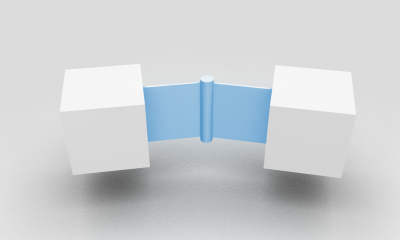
\includegraphics[width=0.7\textwidth]{Revolute_Joint.png}
  \caption{Junta de revolu��o.}
	\label{fig:junta_revolucao}
\end{figure}

Uma das tarefas mais importantes de uma engine F�sica � detectar quais colis�es ocorrem em um dado momento eficientemente. H� dois desafios principais a serem superados nisso: detec��o de colis�o pol�gono por pol�gono (extremamente custosa) e dado \(n\) objetos presentes em uma cena, precisa-se, a princ�pio, testar colis�o entre \(\dbinom{n}{2}\) pares de objetos.

Para resolver o primeiro problema, a \emph{engine} mant�m uma caixa delimitadora (\emph{bounding box}) para cada modelo f�sico. Essa caixa � formada pelos limites m�nimos e m�ximos do modelo em cada uma das coordenadas. Assim, para verificar se dois modelos colidem, o algoritmo verifica primeiro se as caixas delimitadores se sobrep�em; se isso n�o ocorre, pode-se afirmar que os modelos certamente n�o colidem e evita-se o custoso teste pol�gono por pol�gono.

Para evitar testar colis�o entre todos os pares de modelos de uma cena, PhysX divide o espa�o em parti��es, de modo que h� necessidade de verificar colis�es apenas com outros objetos presente na mesma parti��o ou no m�ximo em parti��es vizinhas.

\subsection{UDK Editor}

O \ac{UDK} Editor � a ferramenta principal de edi��o do \ac{UDK}. Por ser uma ferramenta do UDK, ela � voltada � cria��o de jogos. Assim, possui diversas funcionalidades para este fim, como manipula��o de modelos 3D, cria��o de cen�rios etc.

Para esse trabalho, a funcionalidade mais importante � a auto-gera��o de modelos f�sicos a partir de modelos gr�ficos 3D. Para isso, o editor prov� diversos m�todos. Um dos mais convenientes � o K-DOF. O algoritmo do K-DOF basicamente toma K planos alinhados com K eixos passando pelo centro da malha gr�fica e aproxima esses planos o m�ximo poss�vel da malha sem que ocorra intersec��o com esta. Pode-se escolher K dentre as seguintes op��es:

\begin{itemize}
	\item 6: caixa alinhada com os eixos principais (X, Y e Z);
	\item 10: caixa com 4 arestas chanfradas -- pode-se escolher dentre arestas alinhadas com os eixos X, Y ou Z;
	\item 18: caixa com todas as arestas chanfradas;
	\item 26: caixa com todas as arestas e cantos chanfrados.
\end{itemize}

A Figura \ref{fig:kdof} exibe as diferen�as entre as op��es de K-DOF para a pe�a do peito do Robonova.

\begin{figure}[ht!]
	\centering
		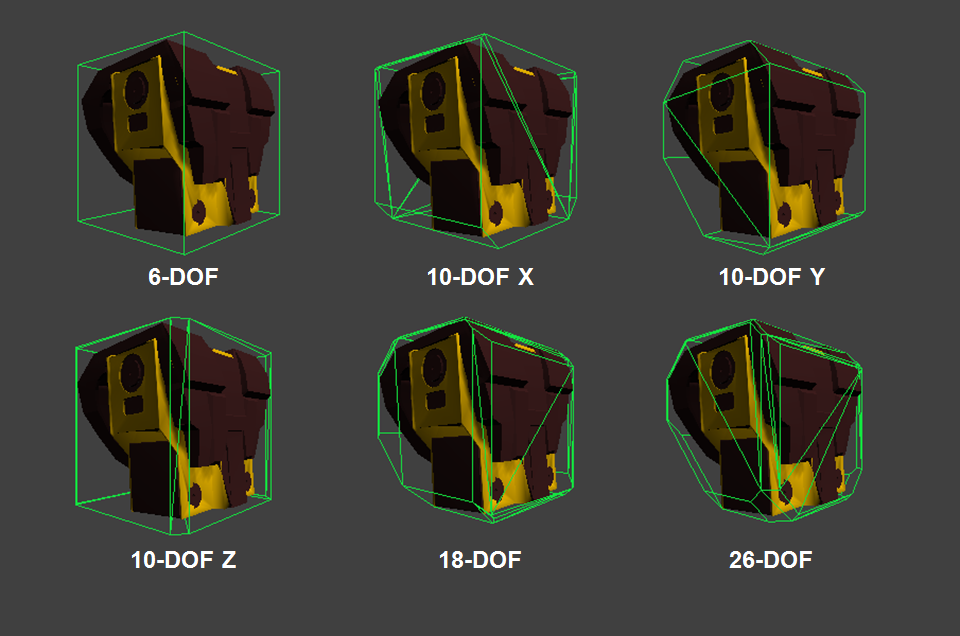
\includegraphics[width=0.8\textwidth]{kdof.png}
  \caption{Diferen�as entre modelos f�sicos gerados com K-DOF (os modelos f�sicos s�o apresentados em \emph{wireframe}).}
	\label{fig:kdof}
\end{figure}

\subsection{UnrealScript}
A UnrealScript � uma linguagem de \emph{script} propriet�ria da \emph{engine} Unreal. Foi projetada por Tim Sweeney especificamente para desenvolvimento de jogos. As principais caracter�sticas da UnrealScript s�o:

\begin{itemize}
	\item Orientada a objetos;
	\item N�o h� suporte a heran�a m�ltipla, ou seja, uma classe s� poder herdar de no m�ximo uma outra classe;
	\item N�o existe o conceito de ponteiro. Trabalha-se com refer�ncias, assim como em Java;
	\item Programador n�o precisa se preocupar com desaloca��o de mem�ria din�mica, pois h� um \emph{garbage collector};
	\item Forte detec��o de erros durante tempo de compila��o;
	\item Estilo de sintaxe similar a C/C++/Java;
	\item Suporte a sobrecarga de operadores;
	\item N�o h� suporte a sobrecarga de m�todos;
	\item Suporte nativo a conceitos importantes para desenvolvimento de jogos: tempo, estados, eventos, propriedades, rede etc.
\end{itemize}
Como pode-se perceber pelas caracter�sticas listadas, muitas das decis�es de projeto da UnrealScript foram inspiradas pela linguagem Java. Inclusive, Tim Sweeney experimentou usar Java para a Unreal antes de decidir criar uma linguagem pr�pria. Por fim, destaca-se que a UnrealScript � usada apenas para programar a parte de alto n�vel. O baixo n�vel, como as partes de renderiza��o gr�fica e de simula��o de F�sica, que exigem mais desempenho, � programado em C++.

\subsection{Implementa��o de Rob�s em USARSim}
A implementa��o de modelos novos de rob�s em USARSim envolve basicamente os passos:

\begin{enumerate}
	\item Constru��o de modelos \acs{CAD} que representam o rob�;
	\item Gera��o dos modelos f�sicos a partir dos modelos \acs{CAD};
	\item Programa��o do modelo do rob� em UnrealScript;
	\item Defini��o de partes extras, como sensores e atuadores.
\end{enumerate}

%O anexo \ref{} apresenta um \emph{tutorial} detalhando o processo.

\subsection{Comunica��o entre Agentes e USARSim}

A comunica��o entre agentes e o simulador � feita atrav�s de trocas de mensagens \acs{TCP/IP} seguindo protocolo pr�prio do \ac{USARSim}. Todas as mensagens trocadas cont�m um tipo e uma lista de segmentos seguindo o formato ``TIPO {segmento1} {segmento2}...'', em que:

\begin{itemize}
	\item TIPO: refere-se ao tipo da mensagem e deve ser escrito em letras ma�usculas. O protocolo define 5 tipos de mensagens: INIT, STA, SEN, DRIVE e CONF;
	\item Segmentos: s�o pares nome-valor escritos da forma ``{nome valor}'' que representam os dados da mensagem em si. Por exemplo, no caso do segmento ``{Orientation 0.0,0.0,0.0}'', ``Orientation'' � o nome e ``0.0,0.0,0.0'' � o valor. 
\end{itemize}

Note que o tipo e a lista de segmentos s�o separados por um espa�o. Os segmentos s�o tamb�m separados entre si por um espa�o. Dentro de um segmento, o nome e valor tamb�m s�o separados por um espa�o, assim espa�os dentro do nome ou do valor n�o s�o permitidos. Com isso, o segmento ``{Orientation 0.0, 0.0, 0.0}'' � inv�lido. Para indicar fim de mensagem, deve-se adicionar ``$\backslash$r$\backslash$n'' no final da cadeia de caracteres.

\section{Robonova-I}
\label{sec:robonova}

O Robonova-I � um modelo de rob� human�ide de baixo custo desenvolvido pela empresa japonesa Hitec Robotics \cite{robonova_manual}. A Figura \ref{fig:robonova} exibe o rob� visto de costas e de frente. O Robonova-I � dotado de 16 graus de liberdade, distribu�dos da seguinte forma: 3 em cada bra�o (2 no ombro e 1 no cotovelo) e 5 em cada perna (2 na coxa, 1 no joelho e 2 no p�). A Figura \ref{fig:juntas_robonova} mostra a disposi��o das juntas, assim como o eixo de rota��o de cada uma.

\begin{figure}[ht!]
	\centering
		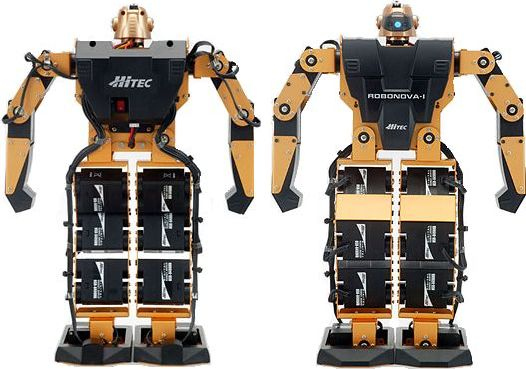
\includegraphics[width=0.8\textwidth]{robonova.jpg}
  \caption{Robonova-I. Extra�do de \cite{robonova_manual}.}
	\label{fig:robonova}
\end{figure}

\begin{figure}[ht!]
	\centering
		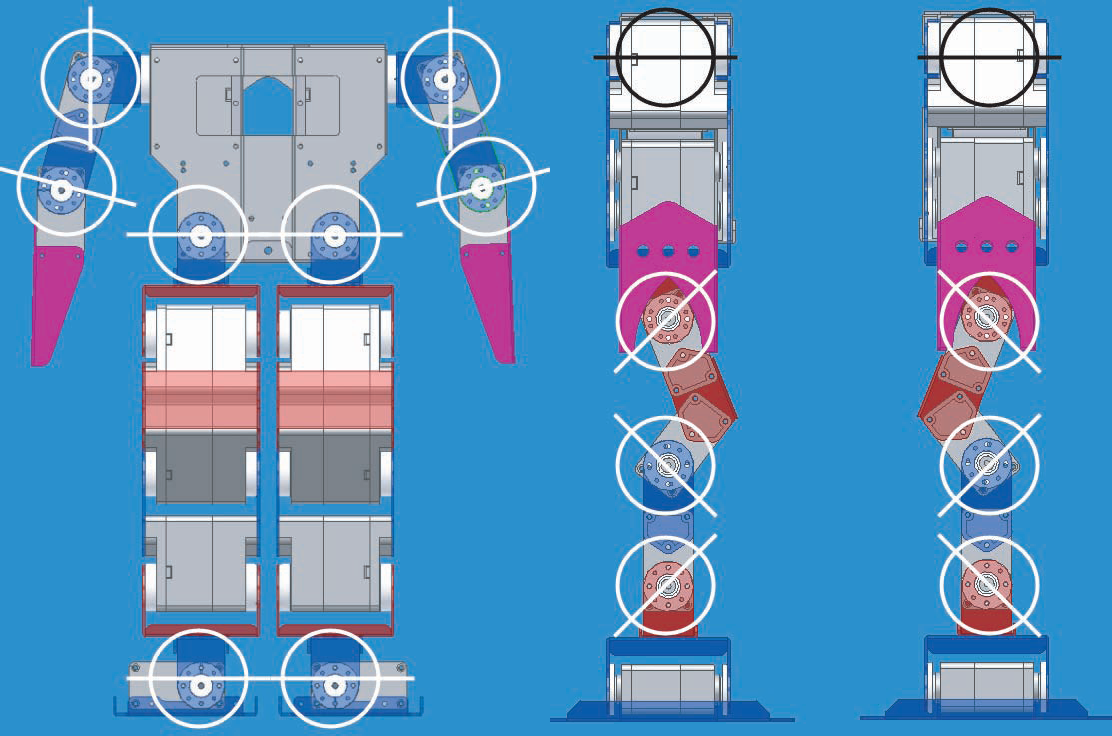
\includegraphics[width=0.8\textwidth]{juntas_robonova.png}
  \caption{Juntas do Robonova-I. Extra�do de \cite{robonova_manual}.}
	\label{fig:juntas_robonova}
\end{figure}

Cada junta � implementada por um servomotor Hitec HSR-8498HB, apresentado na Figura \ref{fig:servos}. Tratam-se de servomotores especificamente desenvolvidos para o Robonova-I e s�o relativamente baratos, o que garante o baixo custo do rob�. A Tabela \ref{tab:servos} apresenta as principais caracter�sticas do HSR-8498HB.

\begin{figure}[ht!]
	\centering
		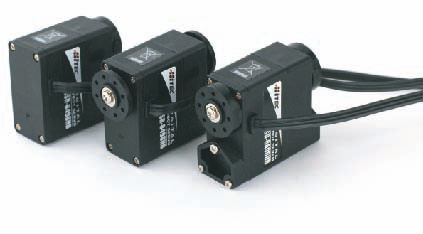
\includegraphics[width=0.5\textwidth]{servos.png}
  \caption{Servomotores Hitec HSR-8498HB. Extra�do de \cite{robonova_manual}.}
	\label{fig:servos}
\end{figure}

\begin{table}[ht!]
  \begin{center}
    \begin{tabular}{| l r |}
    \hline
    Interface & Protocolo \acs{HMI}, \acs{PWM} \\
    Voltagem & 6,0 V \\
    Velocidade M�xima & 60\(^{\circ}\) em 0,20 s @ 6,0 V \\
    Torque & 10 kg\(\cdotp\)cm \\
    �ngulo de Opera��o & M�ximo de 180\(^{\circ}\) \\
    Peso & 55 g \\
    Dimens�o & 40 x 20 x 47 mm \\
    \hline
    \end{tabular}
  \end{center}
  \caption{Especifica��o dos servomotores Hitec HSR-8498HB. Extra�do de \cite{robonova_manual}.}
  \label{tab:servos}
\end{table}

O �nico sensor que vem juntamente com o kit � um sensor infravermelho, que � instalado na cabe�a do rob�, para receber comandos de um controle remoto, que tamb�m faz parte do kit. Por�m, o fabricante produzia alguns tipos de sensores compat�veis, como sensor de toque, gir�metro e sensor de luz.

O controle do rob� � feito por uma placa MR-C3024, que fica instalada nas costas do rob�, conforme mostra a Figura \ref{fig:costas_robonova}. A CPU da placa � um Atmel ATMEGA128, o que � uma limita��o caso se deseje ter um rob� human�ide completamente aut�nomo. O ponto forte da MR-C3024 � ter uma capacidade de \acs{E/S} razo�vel, principalmente suporte a 24 \acsp{PWM}, o que � suficiente para controlar todos os 16 servomotores do kit e ainda permite a adi��o de mais 8. A Tabela \ref{tab:mr-c3024} resume as caracter�sticas da MR-C3024.

\begin{figure}[ht!]
	\centering
		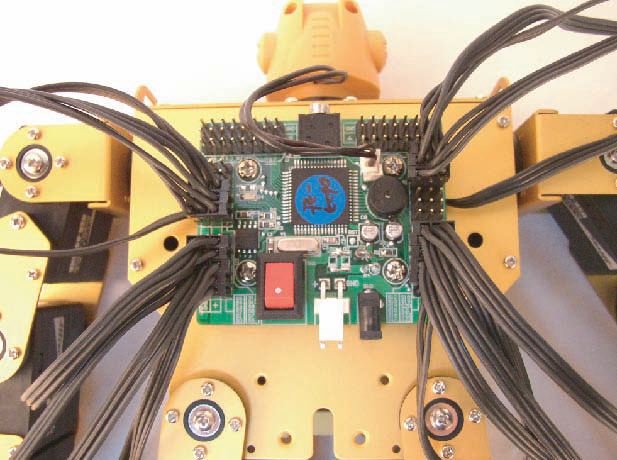
\includegraphics[width=0.8\textwidth]{costas_robonova.png}
  \caption{Detalhe das costas do Robonova-I mostrando a placa MR-C3204 instalada. Extra�do de \cite{robonova_manual}.}
	\label{fig:costas_robonova}
\end{figure}

\begin{table}[ht!]
  \begin{center}
    \begin{tabular}{| l r |}
    \hline
    CPU & Atmel ATMEGA128 8bit RISC \\
    M�x Servos & 24 \\
    Conversores A/D & 8 \\
    Mem�ria de Programa & 32 Kbytes \\
    Peso & 0,2 kg \\
    Dimens�o & 55 x 50 x 15 mm \\
    \hline
    \end{tabular}
  \end{center}
  \caption{Especifica��o da placa MR-C3024. Extra�do de \cite{mr-c3024}.}
  \label{tab:mr-c3024}
\end{table}

A programa��o � feita com uma linguagem propriet�ria chamada RoboBASIC, especificamente criada para o Robonova-I. A linguagem tem a vantagem de possuir primitivas espec�ficas para utilizar os recursos do Robonova-I e da MR-C3024. A programa��o feita � passada do PC para a MR-C3024 por comunica��o serial RS-232 com uso de um cabo pr�prio. Outra op��o de controle � mandar comandos via RS-232 para mover diretamente os servomotores seguindo protocolo pr�prio da MR-C3204 \cite{mr-c3024_protocol}.


\chapter{Modelo de Simula��o}
\section{Modelos CAD}

Os modelos \acs{CAD} foram confeccionados em um trabalho anterior \cite{esther_2007}. Os modelos foram constru�dos com uso do \emph{software} Autodesk AutoCAD \cite{autocad} a partir de medidas das pe�as de do Robonova-I real tomadas com um paqu�metro. Cada pe�a foi feita como um modelo \acs{CAD} separado.

Em seguida, as pe�as foram importados no \emph{software} Autodesk 3D Studio Max \cite{3dsmax}, onde materiais (gr�ficos) com padr�es de cores simples foram criados e assinalados conforme as cores correspondentes no rob� real. As Figuras \ref{fig:robonova_montado_render} e \ref{fig:robonova_explodido_render} apresentam o modelo final montado e o explodido, respectivamente. Como pode-se verificar, teve-se o cuidado de confeccionar o modelo com boa precis�o, para que se consiga um comportamento em simula��o o mais fiel poss�vel ao rob� real.

\begin{figure}[ht!]
	\centering
		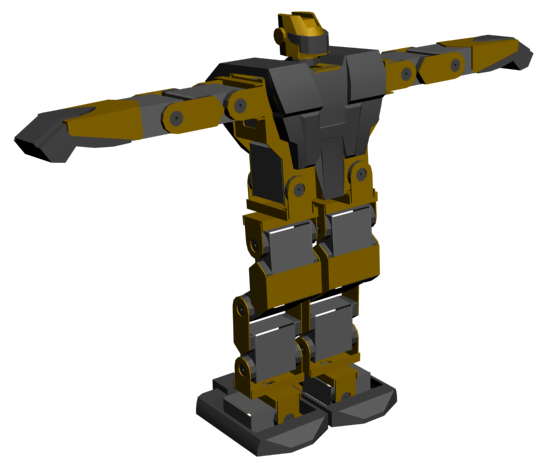
\includegraphics[width=0.5\textwidth]{robonova_montado_render.png}
  \caption{Modelo completo montado do Robonova-I.}
	\label{fig:robonova_montado_render}
\end{figure}

\begin{figure}[ht!]
	\centering
		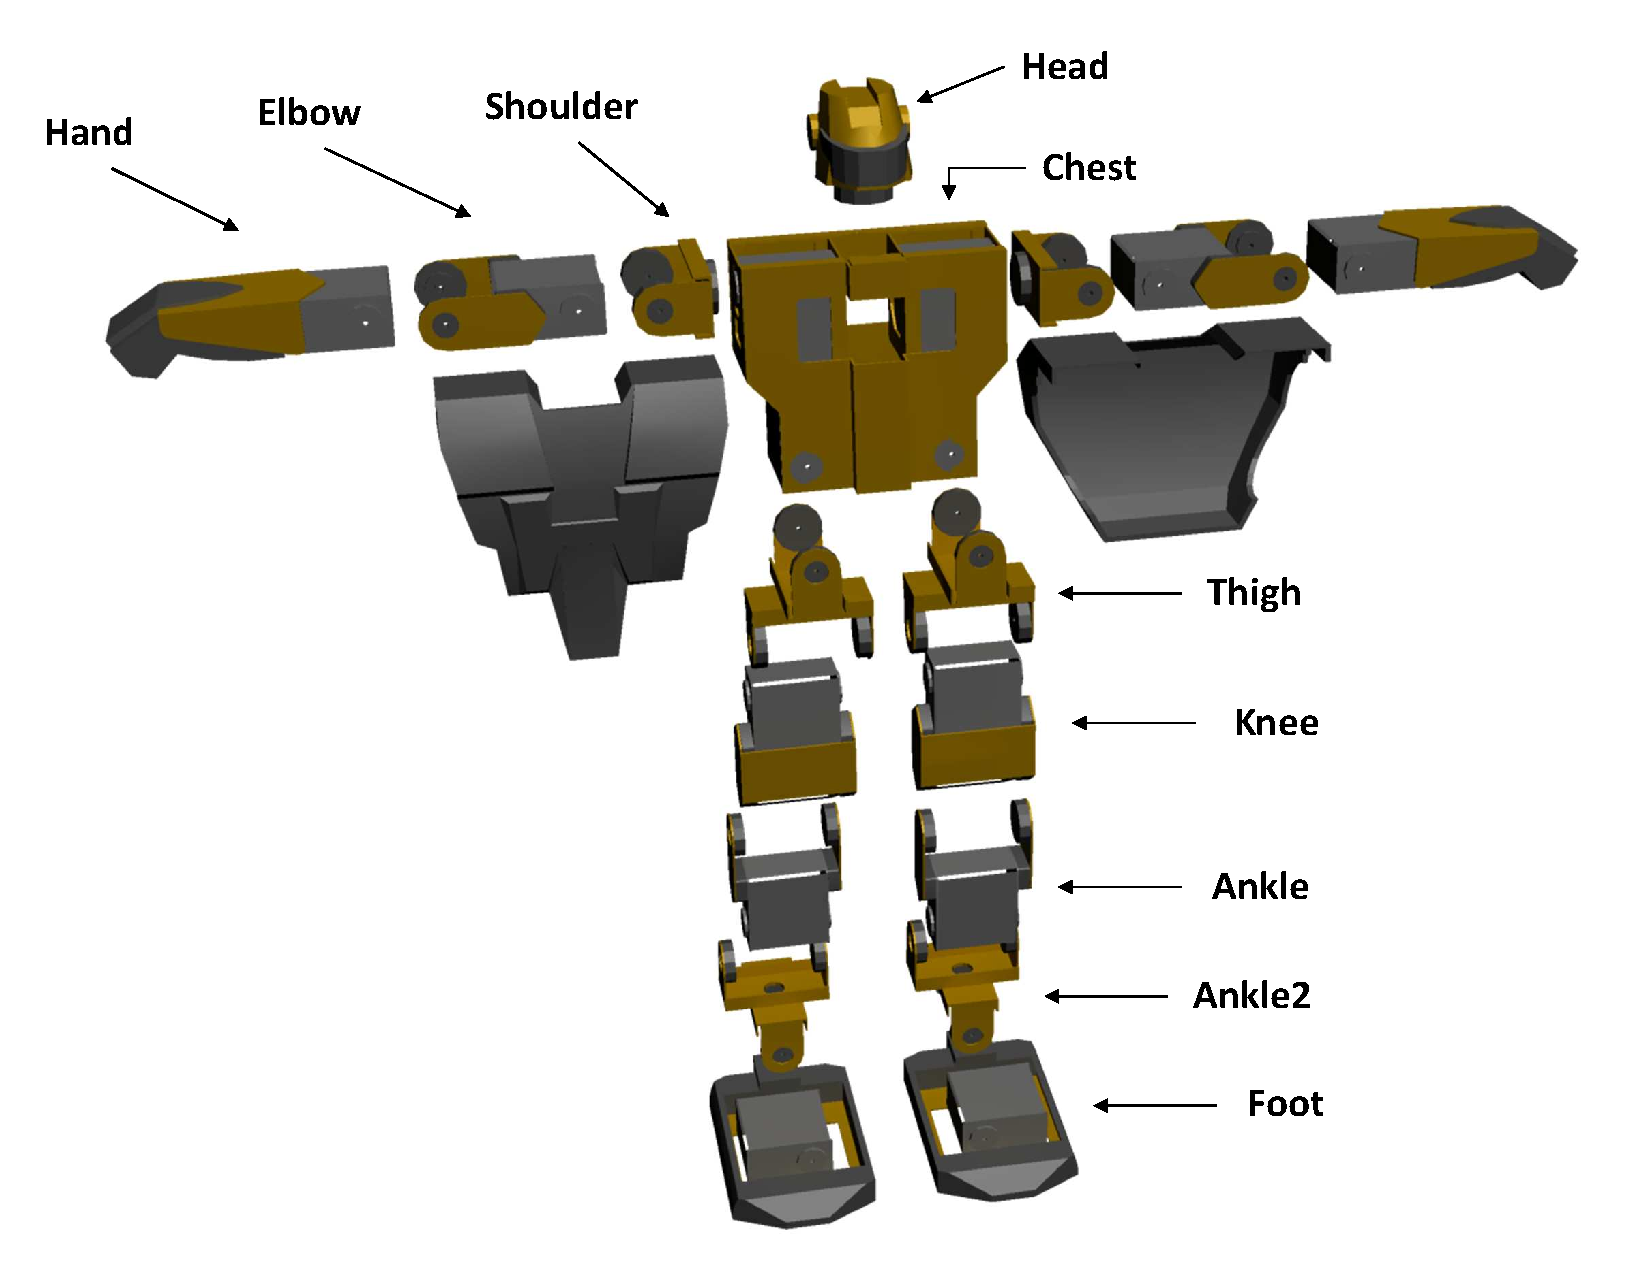
\includegraphics[width=0.8\textwidth]{robonova_explodido_render.pdf}
  \caption{Modelo completo explodido do Robonova-I.}
	\label{fig:robonova_explodido_render}
\end{figure}


Finalmente, cada modelo foi exportado como um arquivo FBX \cite{fbx} separado, porque esse formato permite importa��o direta no \ac{UDK} Editor.

\section{Configura��o no UDK Editor}

Para ter-se um modelo de simula��o o mais fiel poss�vel � realidade, optou-se pelo m�todo \emph{26-DOF simplified collision} para auto-gerar os modelos f�sicos a partir dos gr�ficos.

Embora os materiais j� tivessem sido associados �s pe�as anteriormente, foi necess�rio repetir esse processo dentro do \ac{UDK} Editor. Ap�s a configura��o de todos as pe�as, exportou-se o conjunto de pe�as como um pacote UPK (Unreal Package).

\subsection{Implementa��o no USARSim}

Para concluir a implementa��o do rob� em \ac{USARSim}, faltava ainda criar a classe do rob� em UnrealScript e configurar os sensores. A classe em UnrealScript do Robonova-I foi inspirada na implementa��o em \ac{USARSim} do rob� Albebaran Nao \cite{sander_2012}.

As pe�as foram implementadas como objetos do tipo ``Part'', que permite definir o modelo (gr�fico e f�sico), massa e uma posi��o em rela��o � origem do rob� (ou um deslocamento em rela��o a uma outra Part tomada como ``pai''). A Tabela \ref{tab:parts} apresenta todas as pe�as implementadas.

\begin{table}[tp]
  \begin{center}
    \begin{tabular}{c c}
    \hline
    Pe�a & Massa \\
    (Part) & (g) \\
    \hline
    Head & 27 \\
    Chest & 337 \\
    LeftShoulder & 6 \\
    LeftElbow & 65 \\
    LeftHand & 65 \\
    RightShoulder & 6 \\
    RightElbow & 65 \\
    RightHand & 65 \\
    LeftThigh & 23 \\
    LeftKnee & 135 \\
    LeftAnkle & 44 \\
    LeftAnkle2 & 23 \\
    LeftFoot & 83 \\
    RightThigh & 23 \\
    RightKnee & 135 \\
    RightAnkle & 44 \\
    RightAnkle2 & 23 \\
    RightFoot & 83 \\
    \hline
    \end{tabular}
  \end{center}
  \caption{Pe�as implementadas como objetos do tipo ``Part''.}
  \label{tab:parts}
\end{table}

Em seguida, as juntas foram implementadas como juntas de revolu��o (objetos do tipo ``RevoluteJoint''). Um objeto do tipo RevoluteJoint une dois objetos do tipo Part por um eixo de rota��o. A Figura \ref{fig:joints} mostra os nomes dados �s juntas implementadas.

\begin{figure}[ht!]
	\centering
		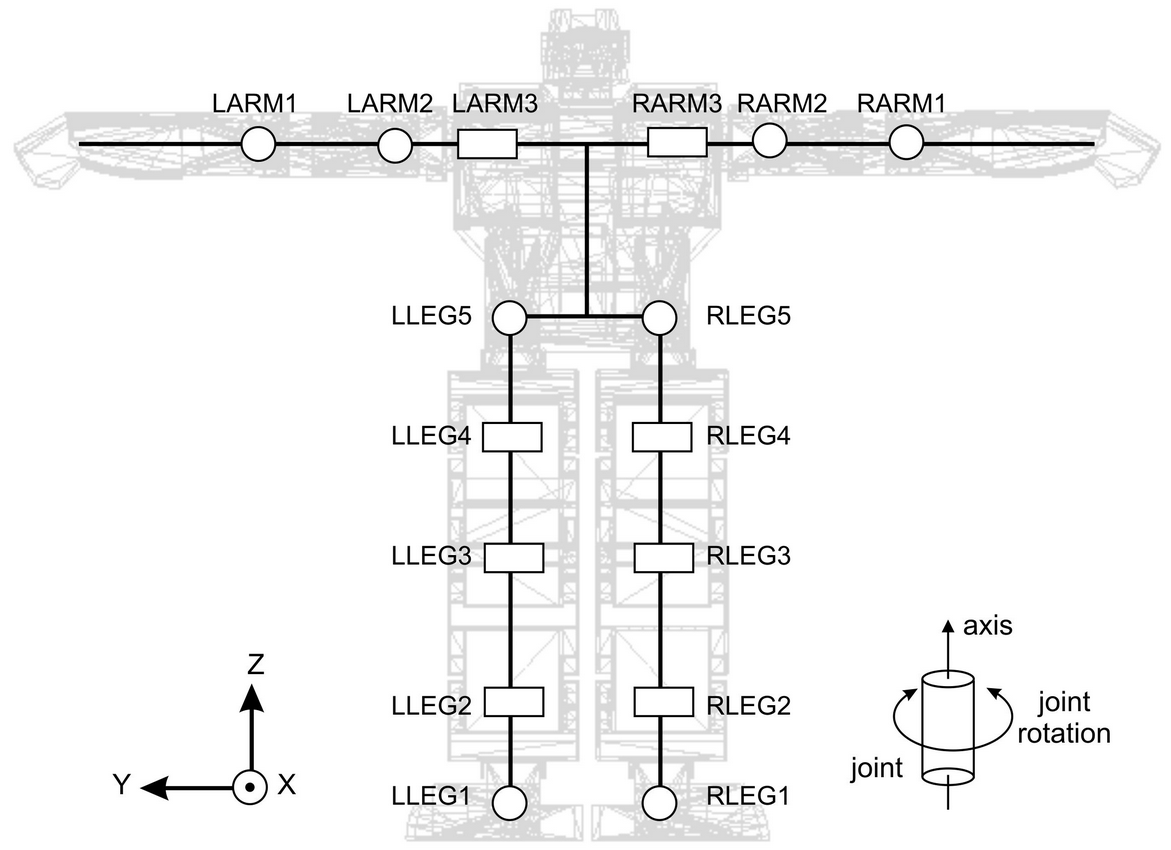
\includegraphics[width=0.7\textwidth]{joints.png}
  \caption{Juntas implementadas no modelo de simula��o.}
	\label{fig:joints}
\end{figure}

Devido a imprecis�es dos modelos f�sicos, foi necess�rio desabilitar colis�o entre pe�as adjacentes (considera-se que duas pe�as s�o adjacentes se s�o ligadas por uma junta). As demais colis�es foram mantidas ativas.

Para percep��o, colocou-se uma c�mera na cabe�a e sensores de toque nos p�s. O \ac{USARSim} j� possui esses sensores implementados, logo foi necess�rio apenas configur�-los. Al�m disso, acoplou-se um sensor especial do \ac{USARSim} chamado ``GroundTruth'' no tronco do rob�. Esse sensor prov� posi��o e orienta��o globais livres de ru�do. Embora essas informa��es sejam imposs�veis de se obter em um rob� real, elas s�o muito �teis em processos de Aprendizado ou Otimiza��o.

A Figura \ref{fig:robonova_simulado} apresenta o Robonova-I dentro do \ac{USARSim}; os modelos f�sicos s�o mostrados em \emph{wireframe} por linhas rosas. No canto superior esquerdo � mostrada a visualiza��o a partir da c�mera do rob�.

\begin{figure}[ht!]
	\centering
		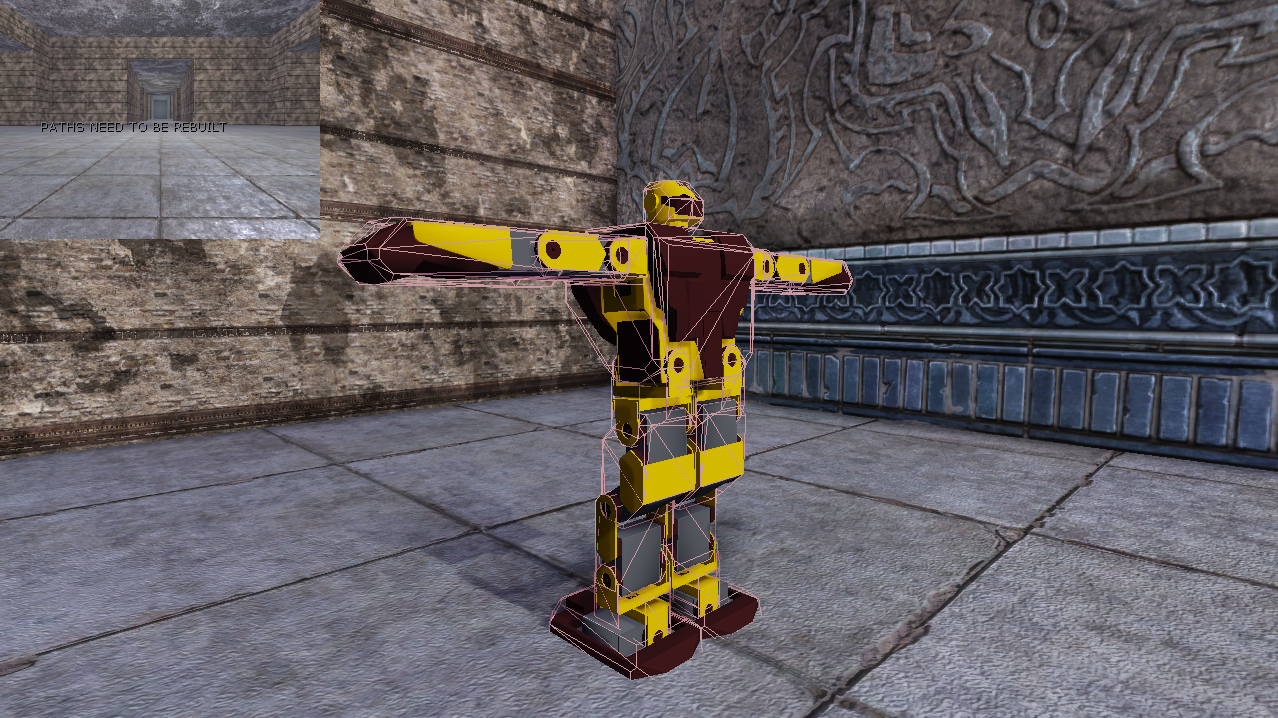
\includegraphics[width=0.8\textwidth]{robonova_simulado.png}
  \caption{Robonova-I simulado dentro do \ac{USARSim}.}
	\label{fig:robonova_simulado}
\end{figure}

\chapter{Programa do Agente}
O agente foi implementado em C++ usando a biblioteca Qt \cite{qt}. Essas tecnologias foram escolhidas pois permitem implementa��o \emph{cross-platform} e um alto desempenho em tempo de execu��o. Para permitir que boa parte do c�digo fosse comum entre simula��o e rob� real, dividiu-se o programa do agente em tr�s camadas (vide Figura \ref{fig:camadas_programa}):

\begin{itemize}
	\item \textbf{Comunica��o:} implementa a comunica��o de baixo n�vel com sensores e atuadores. Interface e implementa��o s�o diferentes entre simula��o e rob� real;
	\item \textbf{Interface:} prov� uma abstra��o para sensores e atuadores. Mesma interface na simula��o e no rob� real, mas implementa��es diferentes;
	\item \textbf{Controlador:} determina quais posi��es devem ser enviadas para as juntas do rob� a cada momento. Interface e implementa��o iguais entre simula��o e rob� real.
\end{itemize}

\begin{figure}[ht!]
	\centering
		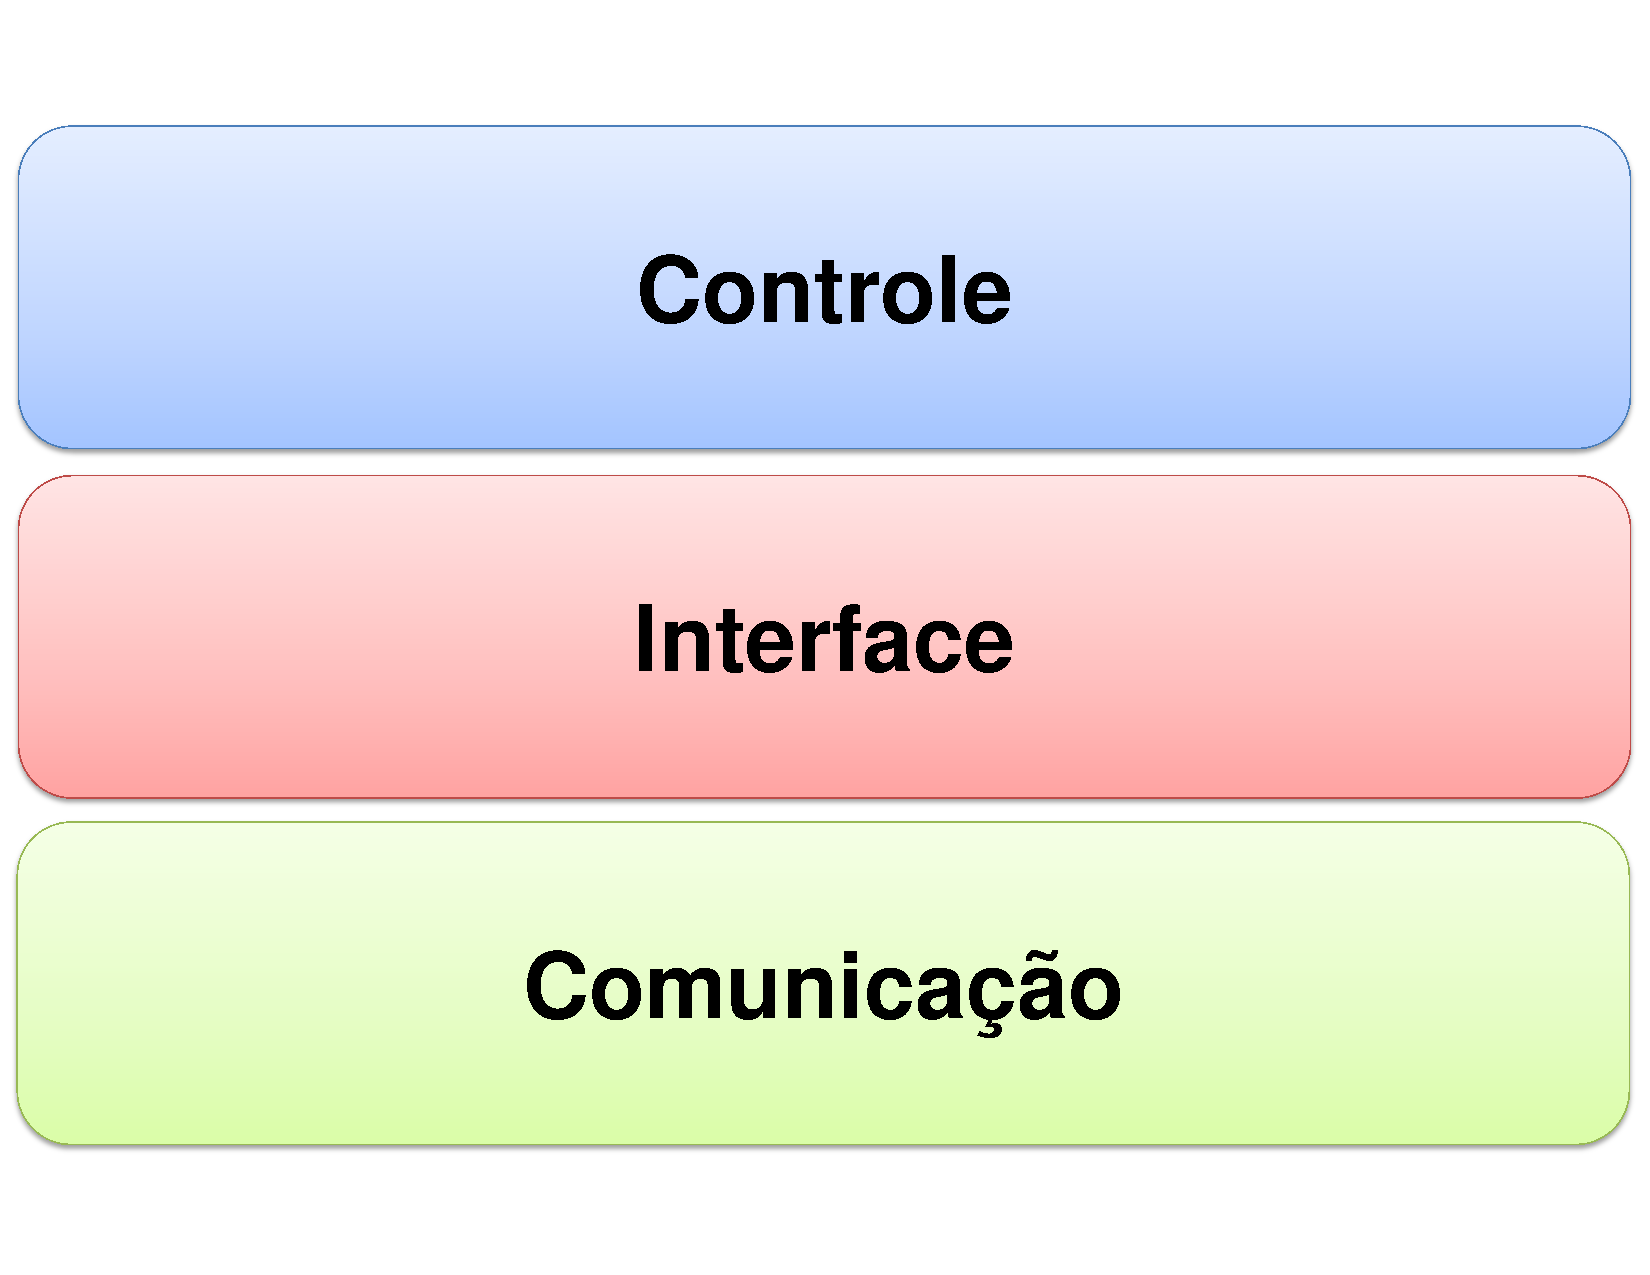
\includegraphics[width=0.5\textwidth]{camadas_programa.pdf}
  \caption{Camadas do programa do agente.}
	\label{fig:camadas_programa}
\end{figure}

� importante observar que a camada de Interface prov� uma abstra��o para a camada superior (Controle), de modo que, a princ�pio, pode-se usar o mesmo controlador para o rob� simulado e para o real. J� as camadas de Comunica��o e de Interface devem ser implementadas em cada plataforma.

Tal arquitetura � suficiente para os prop�sitos desse trabalho. Todavia, caso deseje-se que o rob� realize tarefas mais complexas, como jogar futebol, as seguintes altera��es s�o interessantes:

\begin{itemize}
	\item Adi��o de um componente de \textbf{Modelo} � camada de Controle. Esse componente seria respons�vel por processar as percep��es e gerar modelos mais elaborados sobre o mundo e sobre o agente, de modo a prover informa��es importantes, como posi��es globais do agente, de outros agentes e de objetos. Com isso, seria adequado passar a chamar essa nova camada de \textbf{Modelo e Controle};
	\item Adi��o de uma camada de \textbf{Cogni��o}, que deveria ficar acima das demais. Tal camada trataria de, a partir dos modelos providos pelo componente de Modelo, determinar o melhor movimento (andar, girar o corpo, levantar-se etc.) a ser executado e notificar a camada de Controle disto.
\end{itemize}

A seguir, cada camada efetivamente implementada � detalhada. Nisso, deve-se destacar um fato: fazia parte do plano inicial utilizar o mesmo programa de agente no rob� simulado e no real, tanto que a arquitetura explicada foi idealizada de modo a permitir isso. Entretanto, o �nico \emph{hardware} de processamento disponbilizado foi a placa original do Robonova-I (MR-C3204) que � muito limitada e permite programa��o apenas em linguagem RoboBASIC. Com isso, implementou-se o programa de agente aqui descrito apenas na simula��o.

Embora isto torne a separa��o do programa em camadas irrelevante para a proposta deste trabalho, esta arquitetura ainda � interessante para servir como base para futuros trabalhos em que se possua o \emph{hardware} de processamento necess�rio.

\section{Comunica��o}

A camada de comunica��o implementa a comunica��o direta de baixo n�vel com sensores e atuadores. Como essa comunica��o difere muito entre rob� simulado e real, � dif�cil estabelecer padr�es para essa camada, portanto considerou-se interface e implementa��o diferentes entre as duas plataformas.

Para a simula��o, essa camada deve consistir de um socket \acs{TCP/IP} para comunica��o com o servidor e de um \emph{parser} para transformar as mensagens brutas recebidas em uma estrutura mais f�cil de lidar. Desse modo, a implementa��o � composta por duas classes:

\begin{itemize}
	\item USARSocket: implementa um socket \acs{TCP/IP} para comunica��o com o servidor do \ac{USARSim}. Faz a separa��o dos dados recebidos na comunica��o em mensagens usando a indica��o de fim de mensagem ``$\backslash$r$\backslash$n'', como especificado no protocolo. A funcionalidade de socket propriamente dita � herdada de QTcpSocket, que a implementa de modo \emph{cross-platform};
	\item USARMessage: representa uma mensagem que segue o protocolo do USARSim. A classe possui dois construtores: um que faz o \emph{parsing} de uma mensagem bruta recebida do servidor e a separada em seus constituintes (tipo e segmentos) e outro que recebe os constituientes e gera uma mensagem no protocolo esperado pelo servidor.
\end{itemize}

\section{Interface}

Esta camada trata as estruturas intermedi�rias recebidas da camada de Comunica��o e prov� uma abstra��o para sensores e atuadores independente de se o programa est� sendo executado no rob� simulado ou no real. Como a camada lida com estruturas da camada de Comunica��o, a implementa��o tem de ser diferente entre as duas plataformas. Por�m, como a inten��o � prover uma abstra��o indepente de plataforma para a camada de Controle, a interface deve ser a mesma entre rob� simulado e real.

Para conseguir esse efeito, o mecanismo usado em Orienta��o a Objetos � criar classes abstratas para representar a interface e ent�o criar classes concretas que herdam destas classes abstratas e que implementam as funcionalidades desejadas em cada caso. Portanto, criou-se as seguintes classes abstratas:

\begin{itemize}
	\item RobotPerceptor: funciona como uma esp�cie de sensor especial que cont�m informa��es do corpo do rob�, como n�vel da bateria e posi��es das juntas;
	\item Sensor: representa um sensor gen�rico. Sensores devem ser implementados atrav�s de especializa��o desta classe, com exce��o do RobotPerceptor;
	\item Perception: prov� uma interface �nica para toda a percep��o;
	\item Action: representa uma a��o gen�rica. N�o inclui comandos para as juntas;
	\item ActionHandler: prov� uma interface �nica para toda a atua��o (incluindo as juntas).
\end{itemize}

No rob� simulado, essa camada tem basicamente duas responsabilidades. No lado da percep��o, deve interpretar as estruturas do tipo USARMessage da camada de Comunica��o e atualizar o estado interno do agente. Em rela��o � atua��o, deve receber uma requisi��o para movimenta��o de junta e criar uma estrutura do tipo USARMessage que ser� passada para a camada de Comunica��o. Para isso, as principais classes criadas foram:

\begin{itemize}
	\item GroundTruth: implementa sensor GroundTruth. Sensor exclusivo do rob� simulado;
	\item USARPerception: implementa��o concreta de Perception. Interpreta uma USARMessage recebida da camada de Comunica��o e atualiza o estado interno do rob�;
	\item InitAction: inicia um modelo de rob� na simula��o;
	\item GetStartPosesAction: requisita ao servidor as localiza��es padr�es em que o rob� pode ser iniciado no mapa em quest�o;
	\item ReconnectAction: reconecta o agente ao simulador;
	\item USARActionHandler: implementa��o concreta de ActionHandler. Recebe a��es (incluindo movimenta��o de junta), cria uma USARMessage correspondente e a envia para a camada de Comunica��o.
\end{itemize}

\section{Controle}

O objetivo desta camada � implementar os movimentos do rob� human�ide a partir do controle de suas juntas. Como a camada de Interface prov� uma abstra��o para sensores e atuadores, o c�digo desta camada pode ser o mesmo tanto no rob� simulado quanto no simulado (considerando que o comportamento f�sico do rob� simulado seja pr�ximo o suficiente do real).

Dado o escopo do trabalho, implementou-se apenas um controlador para a caminhada do rob�. Por�m, a implementa��o feita j� prov� uma estrutura para implementa��es futuras de novos movimentos, como girar o corpo, levanta-se, chutar uma bola etc. As principais classes criadas foram:

\begin{itemize}
	\item TFSGaitController: controlador para caminhada baseada em \ac{SFT};
	\item TFSGaitGenerator: classe abstrata que representa um gerador de caminhada baseada em \ac{SFT}. Dado o instante de tempo atual, gera as posi��es das juntas a partir das equa��es do modelo de caminhada.
\end{itemize}

\chapter{Processo de Otimiza��o}
\label{chap:processo_otimizacao}
\section{Modelos de Caminhada}

Para verificar os efeitos da adi��o de movimento de bra�os e movimento no plano coronal, decidiu-se por implementar geradores para os 3 modelos propostos por Shafii \cite{shafii_2010, shafii_2009, shafii_rc}, conforme explicitado no Cap�tulo \ref{chap:locomocao_humanoide}.

Entretanto, ap�s alguns testes, optou-se por modificar a fun��o proposta por Shafii para os ombros. A modifica��o proposta envolve considerar que as amplitudes no sentido positivo e negativo podem ser diferentes para o movimento do bra�o, assim como � feito para a perna no sentido frente-tr�s. Desse modo, \(\theta_o(t)\) passa a ser descrita pela equa��o \eqref{eq:sft_ombro_modificada}.

\begin{equation}
\theta_o(t) =
\begin{cases}
- D_- \sin{\left(\dfrac{2 \pi t}{T}\right)}, & t \in \left[k T, \dfrac{T}{2} + k T\right), k \in \mathbb{Z} \\ \\
- D_+ \sin{\left(\dfrac{2 \pi t}{T}\right)}, & t \in \left[\dfrac{T}{2} + k T, (k+1) T\right), k \in \mathbb{Z}
\end{cases}
\label{eq:sft_ombro_modificada}
\end{equation}

Note que essa modifica��o aumenta em 1 o n�mero de constantes a serem determinadas para os modelos que possuem movimento de bra�os. Portanto, os modelos de caminhada implementados s�o os seguintes:

\begin{itemize}
	\item Modelo Simples (MS): usa apenas as juntas na dire��o frente-tr�s das pernas;
	\item Modelo com Movimento de Bra�os (MB): al�m das juntas do ``Modelo Simples'', utiliza as juntas do ombro (com trajet�ria para o ombro esquerdo definida pela equa��o \eqref{eq:sft_ombro_modificada});
	\item Modelo Complexo (MC): al�m das juntas do Modelo com ``Movimento de Bra�os'', adiciona as juntas da coxa no sentido lateral (plano coronal).
\end{itemize}

Observe que o Robonova possui os graus de liberdade necess�rios para implementar os 3 modelos. A Tabela \ref{tab:mapeamento_juntas} apresenta o mapeamento feito das juntas do modelo te�rico para as do Robonova (veja a Figura \ref{fig:joints} para nomenclatura utilizada para as juntas do Robonova).

\begin{table}[tp]
  \begin{center}
    \begin{tabular}{c c}
    \hline
    Junta nos Modelos Te�ricos & Junta no Robonova \\
    \hline
    Coxa Frente-tr�s Esquerda & LLEG4 \\
    Joelho Esquerdo & LLEG3 \\
    P� Frente-tr�s Esquerdo & LLEG2 \\
    Ombro Esquerdo & LARM3 \\
    Coxa Lateral Esquerda & LLEG5 \\
    P� Lateral Esquerdo & LLEG1 \\
    Coxa Frente-tr�s Direita & RLEG4 \\
    Joelho Direito & RLEG3 \\
    P� Frente-tr�s Direito & RLEG2 \\
    Ombro Direito & RARM3 \\
    Coxa Lateral Direita & RLEG5 \\
    P� Lateral Direito & RLEG1 \\
    \hline
    \end{tabular}
  \end{center}
  \caption{Mapeamento das juntas dos modelos te�ricos para as do Robonova (veja a Figura \ref{fig:joints} para nomenclatura utilizada para as juntas do Robonova).}
  \label{tab:mapeamento_juntas}
\end{table}

\section{Configura��o dos Algoritmos de Otimiza��o}

Um algoritmo de Otimiza��o fornece um \emph{framework} para resolu��o de problemas de otimiza��o, mas deve-se definir o que significa certos elemento do algoritmo para o problema em espec�fico.

O problema de Otimiza��o em quest�o envolve a determina��o de constantes reais relacionada ao modelo de caminhada. � interessante definir um dom�nio para cada uma das constantes a fim de evitar valores sem sentido para o problema (que resultem em �ngulos ou velocidades al�m do dom�nio de opera��o dos servomotores ou que certamente levem � queda do rob�). Ap�s testes manuais, determinou-se os limites para as constantes do modelo apresentados na Tabela \ref{tab:limites_constantes} (as equa��es \eqref{eq:sft_coxa}, \eqref{eq:sft_joelho}, \eqref{eq:sft_ombro_modificada} e \eqref{eq:sft_lateral} apresentam detalhes sobre as constantes mencionadas).

\begin{table}[tph]
  \begin{center}
    \begin{tabular}{c c c}
    \hline
    Constante & M�nimo & M�ximo \\
    \hline
    \(O_c\) &  -1,5 & 0 \\
    \(A\) & 0,01 & 1,0 \\
    \(B\) & 0,01 & 1,0 \\
    \(O_j\) & 0 & 2,0 \\
    \(C\) & 0 & 1,0 \\
    \(\tau = t_2/T\) & 0,1 & 0,9 \\
    \(T\) & 0,1 & 0,7 \\
    \(D_+\) & 0 & 0,6 \\
    \(D_-\) & 0 & 0,6 \\
    \(E\) & 0 & 0,5 \\
    \hline
    \end{tabular}
  \end{center}
  \caption{Limites para os valores das contantes dos modelos de caminhada.}
  \label{tab:limites_constantes}
\end{table}

\subsection{Configura��o do Algoritmo Gen�tico}

A seguir, s�o apresentados como os conceitos de \ac{AG} s�o definidos no problema em espec�fico:

\begin{itemize}
	\item Cromossomo: a escolha mais �bvia para a defini��o de cromossomo � um vetor com as constantes, em que cada gene representa uma constante;
	\item Fun��o de \emph{fitness}: explicitada a seguir, na Se��o \ref{sec:experimento};
	\item Muta��o: altera um gene (no caso, uma das constantes) por um valor real aleat�rio dentro dos limites da Tabela \ref{tab:limites_constantes}.
\end{itemize}

Os demais conceitos de AG (sele��o, \emph{crossover} e sobreviv�ncia dos mais aptos) saem naturalmente da defini��o de cromossomo.

Por fim, a Tabela \ref{tab:parametros_ag} apresenta os valores dos par�metros usados nas execu��es de \ac{AG}.

\begin{table}[tph]
  \begin{center}
    \begin{tabular}{c c c}
    \hline
    Par�metro & Valor \\
    \hline
    \(S_i\) & 20 \\
    \(S_m\) & 20 \\
    \(R\) & 10 \\
    \(p_m\) & 0,05 \\
    \hline
    \end{tabular}
  \end{center}
  \caption{Valores dos par�metros usados nas execu��es de \ac{AG}.}
  \label{tab:parametros_ag}
\end{table}

\subsection{Configura��o do Particle Swarm Optimization}

A escolha natural � considerar que cada part�cula em um espa�o \(n\)-dimensional, em que \(n\) � o n�mero de constantes a serem determinadas. Assim, cada posi��o de part�culas � um vetor de constantes. O espa�o de busca � dado pelos limites da Tabela \ref{tab:limites_constantes}. J� a fun��o de medida de qualidade � apresentada na Se��o \ref{sec:experimento}.

No \ac{PSO} pode ocorrer das part�culas atingirem velocidades muito altas e sa�rem do espa�o de busca. Para evitar esses problemas, fez-se modifica��es no \ac{PSO} apresentado na Se��o \ref{sec:pso}. Primeiramente, logo ap�s a atualiza��o de velocidade deuma part�cula, limita-se sua velocidade com uso da equa��o \eqref{eq:clamp_velocidade}.

\begin{equation}
\boldsymbol{v_i}(d)\gets min(\boldsymbol{u}(d)-\boldsymbol{l}(d), max(\boldsymbol{l}(d)-\boldsymbol{u}(d), \boldsymbol{v_i}(d))), d=1,\ldots ,D
\label{eq:clamp_velocidade}
\end{equation}

A outra modifica��o busca for�ar as part�culas a permanecerem sempre dentro do espa�o de busca. Para tal, considera-se que as part�culas sofrem ``choques mec�nicos inel�sticos'' ao tentarem cruzar os limites do espa�o de busca. A partir desta inspira��o da Mec�nica, criou-se a subrotina apresentada no Algoritmo \ref{alg:choques}, que � executada logo ap�s ser aplicada a limita��o de velocidade. Note que o uso dessa subrotina introduz o par�metro \(\varepsilon\), ao qual deu-se a denomina��o de ``coeficiente de restitui��o'' para seguir a analogia mec�nica.

\begin{algorithm}[H]
\Begin{
\For{$i\gets 1,\ldots,P$} {
	\For{$d\gets 1,\ldots,D$} {
		\If{$\boldsymbol{x_i}(d) > \boldsymbol{u}(d)$}{
			$\delta\gets \boldsymbol{x_i}(d) - \boldsymbol{u}(d)$\;
			$\boldsymbol{x_i}(d)\gets \varepsilon (\boldsymbol{u}(d)-\delta)$\;
			$\boldsymbol{v_i}(d)\gets - \varepsilon \boldsymbol{v_i}(d)$\;
		}
		\If{$\boldsymbol{x_i}(d) < \boldsymbol{l}(d)$}{
			$\delta\gets \boldsymbol{l}(d) - \boldsymbol{x_i}(d)$\;
			$\boldsymbol{x_i}(d)\gets \varepsilon (\boldsymbol{l}(d)+\delta)$\;
			$\boldsymbol{v_i}(d)\gets - \varepsilon \boldsymbol{v_i}(d)$\;
		}
	}
}
}
\caption{Subrotina que simula ``choques'' das part�culas com os limites do espa�o de busca.}
\label{alg:choques}
\end{algorithm}

Por fim, a Tabela \ref{tab:parametros_pso} apresenta os valores dos par�metros usados nas execu��es de \ac{PSO}.

\begin{table}[tph]
  \begin{center}
    \begin{tabular}{c c c}
    \hline
    Par�metro & Valor \\
    \hline
    \(P\) & 20 \\
    \(\omega\) & 0,9 \\
    \(\varphi_p\) & 0,6 \\
    \(\varphi_g\) & 0,8 \\
    \(\varepsilon\) & 0,7 \\
    \hline
    \end{tabular}
  \end{center}
  \caption{Valores dos par�metros usados nas execu��es de \ac{PSO}.}
  \label{tab:parametros_pso}
\end{table}

\section{Montagem do Experimento Simulado}
\label{sec:experimento}

Para utilizar um algoritmo de Otimiza��o para o ``aprendizado'' das melhores constantes para os modelos de caminhada, � necess�rio montar um experimento em que seja dado ao rob� um per�odo de tempo para tentar andar e depois seja aplicada uma m�trica para avalia��o do desempenho da caminhada com o dado conjunto de constantes.

O mapa do simulador escolhido para os experimentos foi o ``ExampleMap'' (vide Figura \ref{fig:examplemap}), porque possui uma grande �rea com terreno plano e sem presen�a de obst�culos. A localiza��o escolhida para iniciar o rob� no mapa foi a ``RobotStart1'', que � onde o rob� se encontra na Figura \ref{fig:examplemap}.

Como o rob� inicia com as juntas em posi��es diferentes das posi��es neutras da caminhada (quando os senos valem zero), adicionou-se um tempo de prepara��o em que os �ngulos das juntas s�o interpolados linearmente das posi��es iniciais para as neutras da caminhada. Experimentalmente, verificou-se que 1,5 segundo era adequado para esse tempo de ajuste.

\begin{figure}[ht!]
	\centering
		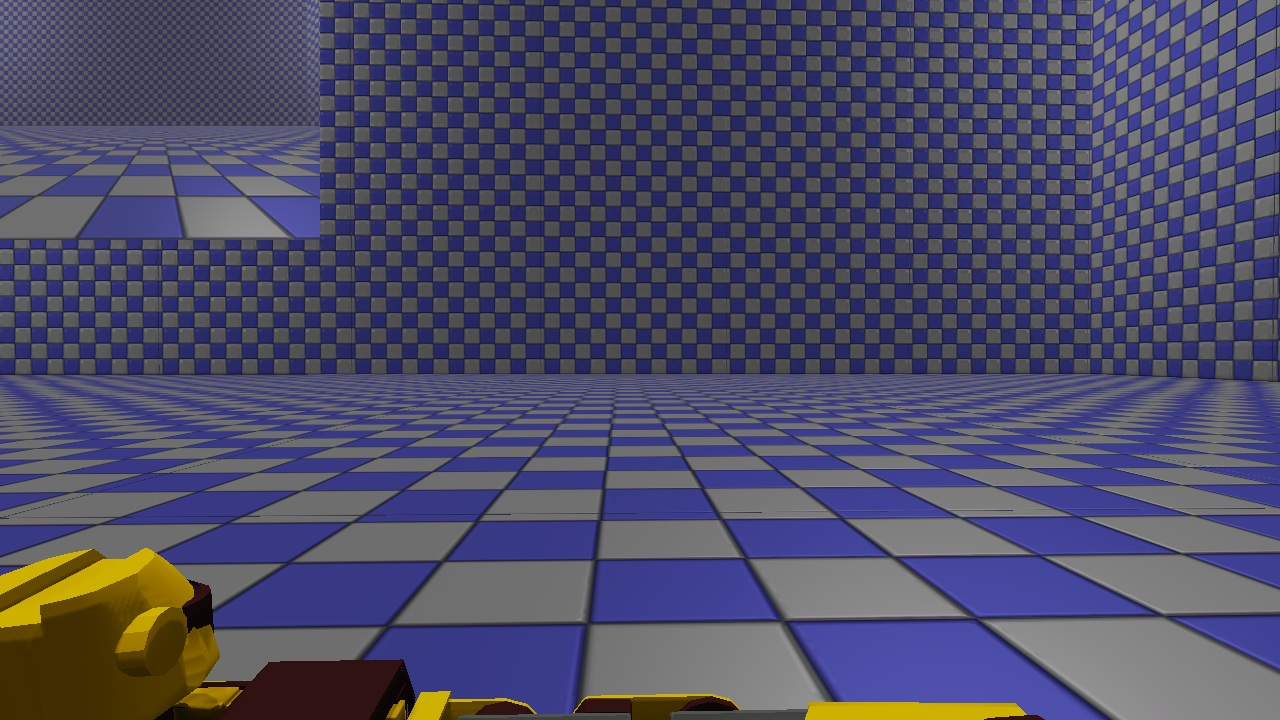
\includegraphics[width=0.8\textwidth]{examplemap.jpg}
  \caption{ExampleMap.}
	\label{fig:examplemap}
\end{figure}

Depois, deixava-se o rob� andar por 20 segundos, o que podia ser interrompido prematuramente caso o rob� ca�sse. Considera-se queda se a orienta��o do rob� passar de 0,6 radianos em rela��o aos eixos X ou Y (vide Figura \ref{fig:examplemap_axes}). Por fim, media-se o desempenho do rob�. Em resumo, cada experimento de simula��o segue os passos:

\begin{enumerate}
	\item Iniciar o Robonova na localiza��o ``RobotStart1'';
	\item Esperar 1,5 segundo para prepara��o;
	\item Esperar 20 segundos ou o rob� cair, o que ocorrer primeiro;
	\item Calcular desempenho com a equa��o \eqref{eq:medida_qualidade}.
\end{enumerate}

\begin{equation}
D = (x-x_o) - |y-y_o| + 0,1\times \Delta t - \sum{P_i}
\label{eq:medida_qualidade}
\end{equation}

Na equa��o \eqref{eq:medida_qualidade}, \((x_o, y_o)\) e \((x, y)\) s�o respectivamente as posi��es inicial e final do rob� no plano do mapa; o sistema de coordenadas usado � o mostrado na Figura \ref{fig:examplemap_axes}. \(\Delta t\) � a quantidade tempo (em segundos) que o rob� permaneceu sem cair. \(\sum{P_i}\) representa o somat�rio das poss�veis puni��es (mostradas na Tabela \ref{tab:punicoes}). O objetivo das puni��es � tratar casos muito indesejados.

\begin{figure}[ht!]
	\centering
		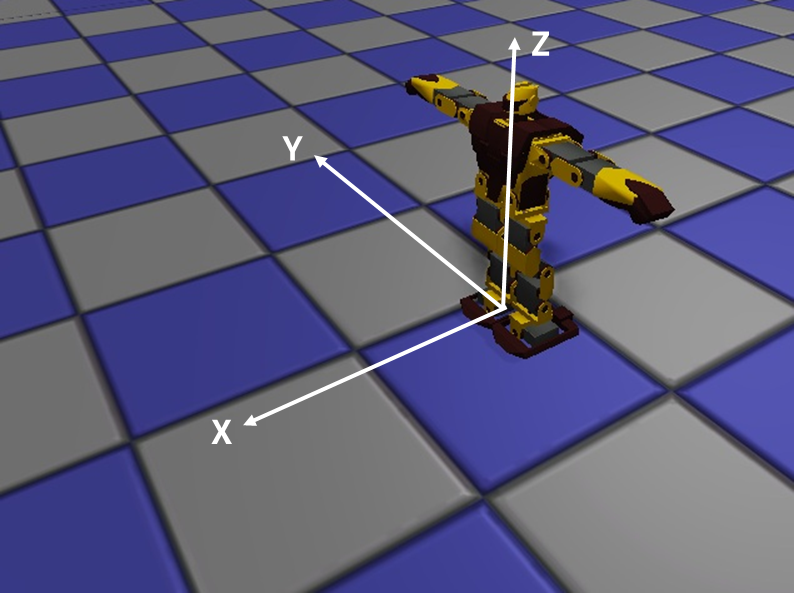
\includegraphics[width=0.5\textwidth]{examplemap_axes.png}
  \caption{Sistema de coordenadas no USARSim.}
	\label{fig:examplemap_axes}
\end{figure}

\begin{table}[tph]
  \begin{center}
    \begin{tabular}{c c c}
    \hline
    Puni��o & Significado & Valor \\
    \hline
    \(P_1\) & Queda & 50 \\
    \(P_2\) & Posi��o inicial inst�vel & 80 \\
    \(P_3\) & Praticamente n�o se moveu & 60 \\
    \hline
    \end{tabular}
  \end{center}
  \caption{Limites para os valores das contantes dos modelos de caminhada.}
  \label{tab:punicoes}
\end{table}

Ap�s algumas execu��es dos experimentos simulados, verificou-se o seguinte:

\begin{itemize}
	\item Percebeu-se que havia uma dificuldade grande do rob� romper a transi��o brusca de quando ele estava parado para o primeiro passo. Ocorria com frequ�ncia de uma caminhada que se tornava bem est�vel quando o rob� entrava em regime cair no primeiro passo;
	\item �s vezes, ocorria de uma caminhada pouco est�vel, mas muito r�pida, ter a sorte de se manter em p� durante os 20 segundos do teste e receber uma avalia��o muito boa. Isto era problem�tico principalmente para o \ac{PSO}, que � fortemente guiado pelo melhor desempenho encontrado.
\end{itemize}

Para resolver estes dois problemas, implementou-se duas heur�sticas propostas em \cite{shafii_rc}:

\begin{itemize}
	\item Ao inv�s de come�ar o movimento j� com as amplitudes no m�ximo, no come�o do movimento reduz-se todas as amplitudes dos movimentos por um fator que aumenta linearmente de 0 a 1. Ap�s alguns testes, determinou-se que uma dura��o de 3 per�odos (3 primeiros passos) era adequada para este tempo. Ou seja, o rob� come�a dando passos curtos e vai aumentando o tamanho do passo gradativamente at� atingir o valor de regime;
	\item Ao inv�s de usar o desempenho de uma �nica execu��o do experimento para alimentar a otimiza��o, passou-se a utilizar uma m�dia de 3 execu��es.
\end{itemize}

\section{Resultados e Discuss�es}

A Tabela \ref{tab:resultados} apresenta os resultados dos experimentos. Como \ac{AG} e \ac{PSO} envolvem aleatoriedade, o mais justo para compara��o seria realizar diversas execu��es de cada algoritmo para cada modelo de caminhada e tirar uma m�dia. Entretanto, isso exigiria uma disponibilidade de poder de processamento bem superior � que o autor tinha dispon�vel. Assim, cada linha da Tabela \ref{tab:resultados} se refere a uma �nica inst�ncia de execu��o. Apesar disso, acredita-se que os resultados apresentados permitem fazer as seguintes considera��es qualitativas:

\begin{itemize}
	\item A adi��o de movimento de bra�os provoca melhora na qualidade da caminhada (se os par�metros estiverem ajustados corretamente);
	\item A adi��o de movimento no plano coronal provoca melhora ainda maior na qualidade da caminhada (novamente, se os par�metros estiverem ajustados corretamente);
	\item Quanto mais par�metros s�o adicionados ao modelo, mais dif�cil � a converg�ncia dos algoritmos, como esperado.
\end{itemize}

\begin{table}[tph]
  \begin{center}
    \begin{tabular}{c c c c}
    \hline
    Algoritmo & Modelo & Melhor & N�mero \\
    de Otimiza��o & de Caminhada & Desempenho & de Testes \\
    \hline
    AG & Simples & 6,16 & 1585 \\
    AG & Com Movimento de Bra�os & 8,3 & 1678 \\
    AG & Complexo & 5,77 & 1636 \\
    PSO & Simples & 5,58 & 860 \\
    PSO & Com Movimento de Bra�os & 7,2 & 1449 \\
    PSO & Complexo & 7,99 & 1493 \\
    \hline
    \end{tabular}
  \end{center}
  \caption{Resultados dos Experimentos.}
  \label{tab:resultados}
\end{table}

As Figuras \ref{fig:convergencia_ag_simples}, \ref{fig:convergencia_ag_bracos} e \ref{fig:convergencia_ag_complexo} apresentam como varia o melhor \emph{fitness} at� ent�o pelo n�mero de testes para experimentos com AG. As Figuras \ref{fig:convergencia_pso_simples}, \ref{fig:convergencia_pso_bracos} e \ref{fig:convergencia_pso_complexo} fazem o mesmo para o PSO. A Tabela \ref{tab:melhores_otimizacao} exibem os melhores conjuntos de par�metros encontrados para cada caso.

\begin{figure}[ht!]
	\centering
	\newlength\figureheight 
	\newlength\figurewidth
	\setlength\figureheight{0.4\textwidth}
	\setlength\figurewidth{0.7\textwidth}
	% This file was created by matlab2tikz v0.2.3.
% Copyright (c) 2008--2012, Nico Schlömer <nico.schloemer@gmail.com>
% All rights reserved.
% 
% The latest updates can be retrieved from
%   http://www.mathworks.com/matlabcentral/fileexchange/22022-matlab2tikz
% where you can also make suggestions and rate matlab2tikz.
% 
% 
% 
\begin{tikzpicture}

\begin{axis}[%
view={0}{90},
width=4.52083333333333in,
height=3.565625in,
scale only axis,
xmin=0, xmax=1600,
xlabel={N�mero de testes},
ymin=-20, ymax=10,
ylabel={Melhor desempenho}]
\addplot [
color=blue,
solid,
forget plot
]
coordinates{
 (1,-17.8431)(2,-17.8431)(3,-17.8431)(4,-17.8431)(5,-17.8431)(6,-17.8431)(7,-17.8431)(8,-17.8431)(9,-17.8431)(10,-17.8431)(11,-17.8431)(12,-17.8431)(13,-17.8431)(14,-17.8431)(15,-17.8431)(16,-17.8431)(17,-17.8431)(18,-17.8431)(19,-17.8431)(20,-17.8431)(21,2.022)(22,2.40803)(23,2.40803)(24,2.40803)(25,2.40803)(26,2.40803)(27,2.40803)(28,2.40803)(29,2.40803)(30,2.40803)(31,2.40803)(32,2.40803)(33,2.40803)(34,2.40803)(35,2.40803)(36,2.40803)(37,2.40803)(38,2.40803)(39,2.40803)(40,2.40803)(41,2.40803)(42,2.40803)(43,2.40803)(44,2.40803)(45,2.40803)(46,2.40803)(47,2.40803)(48,2.40803)(49,2.40803)(50,2.40803)(51,2.40803)(52,2.40803)(53,2.40803)(54,2.40803)(55,2.40803)(56,2.40803)(57,2.40803)(58,2.40803)(59,2.40803)(60,2.40803)(61,2.40803)(62,2.40803)(63,2.40803)(64,2.40803)(65,2.40803)(66,2.40803)(67,2.40803)(68,2.40803)(69,2.40803)(70,2.40803)(71,2.40803)(72,2.40803)(73,2.40803)(74,2.40803)(75,2.40803)(76,2.40803)(77,2.40803)(78,2.40803)(79,2.40803)(80,2.40803)(81,2.40803)(82,2.40803)(83,2.40803)(84,2.40803)(85,2.40803)(86,2.40803)(87,3.59803)(88,3.59803)(89,3.59803)(90,3.59803)(91,3.59803)(92,3.59803)(93,3.59803)(94,3.59803)(95,3.59803)(96,3.59803)(97,3.59803)(98,3.59803)(99,3.59803)(100,3.59803)(101,3.59803)(102,3.59803)(103,3.59803)(104,3.59803)(105,3.59803)(106,3.59803)(107,3.59803)(108,3.59803)(109,3.59803)(110,3.59803)(111,3.59803)(112,3.59803)(113,3.59803)(114,3.59803)(115,3.59803)(116,3.59803)(117,3.59803)(118,3.59803)(119,3.59803)(120,3.59803)(121,3.59803)(122,3.59803)(123,3.59803)(124,3.59803)(125,3.59803)(126,3.59803)(127,3.59803)(128,3.59803)(129,3.59803)(130,3.59803)(131,3.59803)(132,3.59803)(133,3.59803)(134,3.59803)(135,3.59803)(136,3.59803)(137,3.59803)(138,3.59803)(139,3.59803)(140,3.59803)(141,3.59803)(142,3.59803)(143,3.59803)(144,3.59803)(145,3.59803)(146,3.59803)(147,3.59803)(148,3.59803)(149,3.59803)(150,3.59803)(151,3.59803)(152,3.59803)(153,3.59803)(154,3.59803)(155,3.59803)(156,3.59803)(157,3.59803)(158,3.59803)(159,3.59803)(160,3.59803)(161,3.59803)(162,3.59803)(163,3.59803)(164,3.59803)(165,3.59803)(166,3.59803)(167,3.59803)(168,3.59803)(169,3.59803)(170,3.59803)(171,3.59803)(172,3.59803)(173,3.59803)(174,3.59803)(175,3.59803)(176,3.59803)(177,3.59803)(178,3.59803)(179,3.59803)(180,3.59803)(181,3.59803)(182,3.59803)(183,3.59803)(184,3.59803)(185,3.59803)(186,3.59803)(187,3.59803)(188,3.59803)(189,3.59803)(190,3.59803)(191,3.59803)(192,3.59803)(193,3.59803)(194,3.59803)(195,3.59803)(196,3.59803)(197,3.59803)(198,3.59803)(199,3.59803)(200,3.59803)(201,3.59803)(202,3.59803)(203,3.59803)(204,3.59803)(205,3.59803)(206,3.59803)(207,3.59803)(208,3.59803)(209,3.59803)(210,3.59803)(211,3.59803)(212,3.59803)(213,3.59803)(214,3.59803)(215,3.59803)(216,3.59803)(217,3.59803)(218,3.59803)(219,3.59803)(220,3.59803)(221,3.59803)(222,3.59803)(223,3.59803)(224,3.59803)(225,3.59803)(226,3.59803)(227,3.59803)(228,3.59803)(229,3.59803)(230,3.59803)(231,3.59803)(232,3.59803)(233,3.59803)(234,3.59803)(235,3.59803)(236,3.59803)(237,3.59803)(238,3.59803)(239,3.59803)(240,3.59803)(241,3.59803)(242,3.59803)(243,3.59803)(244,3.59803)(245,3.59803)(246,3.59803)(247,3.59803)(248,3.59803)(249,3.59803)(250,3.59803)(251,3.59803)(252,3.59803)(253,3.59803)(254,3.59803)(255,3.59803)(256,3.59803)(257,3.59803)(258,3.59803)(259,3.59803)(260,3.59803)(261,3.59803)(262,3.59803)(263,3.59803)(264,3.59803)(265,3.59803)(266,3.59803)(267,3.59803)(268,3.59803)(269,3.59803)(270,3.59803)(271,3.59803)(272,3.59803)(273,3.59803)(274,3.59803)(275,3.59803)(276,3.59803)(277,3.59803)(278,3.59803)(279,3.59803)(280,3.59803)(281,3.59803)(282,3.59803)(283,3.59803)(284,3.59803)(285,3.59803)(286,3.59803)(287,3.59803)(288,3.59803)(289,3.59803)(290,3.59803)(291,3.59803)(292,3.59803)(293,3.59803)(294,3.59803)(295,3.59803)(296,3.59803)(297,3.59803)(298,3.59803)(299,3.59803)(300,3.59803)(301,3.59803)(302,3.59803)(303,3.59803)(304,3.59803)(305,3.59803)(306,3.59803)(307,3.59803)(308,3.59803)(309,3.59803)(310,3.59803)(311,3.59803)(312,3.59803)(313,3.59803)(314,3.59803)(315,3.59803)(316,3.59803)(317,3.59803)(318,3.59803)(319,3.59803)(320,3.59803)(321,3.59803)(322,3.59803)(323,3.59803)(324,3.59803)(325,3.59803)(326,3.59803)(327,3.59803)(328,3.59803)(329,3.59803)(330,3.59803)(331,3.59803)(332,3.59803)(333,3.59803)(334,3.59803)(335,3.59803)(336,3.59803)(337,3.59803)(338,3.59803)(339,3.59803)(340,3.59803)(341,3.59803)(342,3.59803)(343,3.59803)(344,3.59803)(345,3.59803)(346,3.59803)(347,3.59803)(348,3.59803)(349,3.59803)(350,3.59803)(351,3.59803)(352,3.59803)(353,3.59803)(354,3.59803)(355,3.59803)(356,3.59803)(357,3.59803)(358,3.59803)(359,3.59803)(360,3.59803)(361,3.59803)(362,3.59803)(363,3.59803)(364,3.59803)(365,3.59803)(366,3.59803)(367,3.59803)(368,3.59803)(369,3.59803)(370,3.59803)(371,3.59803)(372,3.59803)(373,3.59803)(374,3.59803)(375,3.59803)(376,3.59803)(377,3.59803)(378,3.59803)(379,3.59803)(380,3.59803)(381,3.59803)(382,3.59803)(383,3.59803)(384,3.59803)(385,3.59803)(386,3.59803)(387,3.59803)(388,3.59803)(389,3.59803)(390,3.59803)(391,3.59803)(392,3.59803)(393,3.59803)(394,3.59803)(395,3.59803)(396,3.59803)(397,3.59803)(398,3.59803)(399,3.59803)(400,3.59803)(401,3.59803)(402,3.59803)(403,3.59803)(404,3.59803)(405,3.59803)(406,3.59803)(407,3.59803)(408,3.59803)(409,3.59803)(410,3.59803)(411,3.59803)(412,3.59803)(413,3.59803)(414,3.59803)(415,3.59803)(416,3.59803)(417,3.59803)(418,3.59803)(419,3.59803)(420,3.59803)(421,3.59803)(422,3.59803)(423,3.59803)(424,3.59803)(425,3.59803)(426,3.59803)(427,3.59803)(428,3.59803)(429,3.59803)(430,3.59803)(431,3.59803)(432,3.59803)(433,3.59803)(434,3.59803)(435,3.59803)(436,3.59803)(437,3.59803)(438,3.59803)(439,3.59803)(440,3.59803)(441,3.59803)(442,3.59803)(443,3.59803)(444,3.59803)(445,3.59803)(446,3.59803)(447,3.59803)(448,3.59803)(449,3.59803)(450,3.59803)(451,3.59803)(452,3.59803)(453,3.59803)(454,3.59803)(455,3.59803)(456,3.59803)(457,3.59803)(458,3.59803)(459,3.59803)(460,3.59803)(461,3.59803)(462,3.59803)(463,3.59803)(464,3.59803)(465,3.59803)(466,3.59803)(467,3.59803)(468,3.59803)(469,3.59803)(470,3.59803)(471,3.59803)(472,3.59803)(473,3.59803)(474,3.59803)(475,3.59803)(476,3.59803)(477,3.59803)(478,3.59803)(479,3.59803)(480,3.59803)(481,3.59803)(482,3.59803)(483,3.59803)(484,3.59803)(485,3.59803)(486,3.59803)(487,3.59803)(488,3.59803)(489,3.59803)(490,3.59803)(491,3.59803)(492,3.59803)(493,3.59803)(494,3.59803)(495,3.59803)(496,3.59803)(497,3.59803)(498,3.59803)(499,3.59803)(500,3.59803)(501,3.59803)(502,3.59803)(503,3.59803)(504,3.59803)(505,3.59803)(506,3.59803)(507,3.59803)(508,3.59803)(509,3.59803)(510,3.59803)(511,3.59803)(512,3.59803)(513,3.59803)(514,3.59803)(515,3.59803)(516,3.59803)(517,3.59803)(518,3.59803)(519,3.59803)(520,3.59803)(521,3.59803)(522,3.59803)(523,3.59803)(524,3.59803)(525,3.59803)(526,3.59803)(527,3.59803)(528,3.59803)(529,3.59803)(530,3.59803)(531,3.59803)(532,3.59803)(533,3.59803)(534,3.59803)(535,3.59803)(536,3.59803)(537,3.59803)(538,3.59803)(539,3.59803)(540,3.59803)(541,3.59803)(542,3.59803)(543,3.59803)(544,3.59803)(545,3.59803)(546,3.59803)(547,3.59803)(548,3.59803)(549,3.59803)(550,3.59803)(551,3.59803)(552,3.59803)(553,3.59803)(554,3.59803)(555,3.59803)(556,3.59803)(557,3.59803)(558,3.59803)(559,3.59803)(560,3.59803)(561,3.59803)(562,3.59803)(563,3.59803)(564,3.59803)(565,3.59803)(566,3.59803)(567,3.59803)(568,3.59803)(569,3.59803)(570,3.59803)(571,3.59803)(572,3.59803)(573,3.59803)(574,3.59803)(575,3.59803)(576,3.59803)(577,3.59803)(578,3.59803)(579,3.59803)(580,3.64867)(581,3.64867)(582,3.64867)(583,3.64867)(584,3.64867)(585,3.64867)(586,3.64867)(587,3.64867)(588,3.64867)(589,3.64867)(590,3.64867)(591,3.64867)(592,3.64867)(593,3.64867)(594,3.64867)(595,3.64867)(596,3.64867)(597,3.64867)(598,3.64867)(599,3.64867)(600,3.64867)(601,3.64867)(602,3.64867)(603,3.64867)(604,3.64867)(605,3.64867)(606,3.64867)(607,3.64867)(608,3.64867)(609,3.64867)(610,3.64867)(611,3.64867)(612,3.64867)(613,3.64867)(614,3.64867)(615,3.64867)(616,3.64867)(617,3.64867)(618,3.64867)(619,3.64867)(620,3.64867)(621,3.64867)(622,3.64867)(623,3.64867)(624,3.64867)(625,3.64867)(626,3.64867)(627,3.64867)(628,3.64867)(629,3.64867)(630,3.64867)(631,3.64867)(632,3.64867)(633,3.64867)(634,3.64867)(635,3.64867)(636,3.64867)(637,3.64867)(638,3.64867)(639,3.64867)(640,3.64867)(641,3.64867)(642,3.64867)(643,3.64867)(644,3.64867)(645,3.64867)(646,3.64867)(647,3.64867)(648,3.64867)(649,3.64867)(650,3.64867)(651,3.64867)(652,3.64867)(653,3.64867)(654,3.64867)(655,3.64867)(656,3.64867)(657,3.64867)(658,3.64867)(659,3.64867)(660,3.64867)(661,3.64867)(662,3.64867)(663,3.64867)(664,3.64867)(665,3.64867)(666,3.64867)(667,3.64867)(668,3.64867)(669,3.64867)(670,3.64867)(671,3.64867)(672,3.64867)(673,3.64867)(674,3.64867)(675,3.64867)(676,3.64867)(677,3.64867)(678,3.64867)(679,3.64867)(680,3.64867)(681,3.64867)(682,3.64867)(683,3.64867)(684,3.64867)(685,3.64867)(686,3.64867)(687,3.64867)(688,3.64867)(689,3.64867)(690,3.64867)(691,3.64867)(692,3.64867)(693,3.64867)(694,3.64867)(695,3.64867)(696,3.64867)(697,3.64867)(698,3.64867)(699,3.64867)(700,3.64867)(701,3.64867)(702,3.64867)(703,3.64867)(704,3.64867)(705,3.64867)(706,3.64867)(707,3.64867)(708,3.64867)(709,3.64867)(710,3.64867)(711,3.64867)(712,3.64867)(713,3.64867)(714,3.64867)(715,3.64867)(716,3.64867)(717,3.64867)(718,3.64867)(719,3.64867)(720,3.64867)(721,3.64867)(722,3.64867)(723,3.64867)(724,3.64867)(725,3.64867)(726,3.64867)(727,3.64867)(728,3.64867)(729,3.64867)(730,3.64867)(731,3.64867)(732,3.64867)(733,3.64867)(734,3.64867)(735,3.64867)(736,3.64867)(737,3.64867)(738,3.64867)(739,3.64867)(740,3.64867)(741,3.64867)(742,3.64867)(743,3.64867)(744,3.64867)(745,3.64867)(746,3.64867)(747,3.64867)(748,3.64867)(749,3.64867)(750,3.64867)(751,3.64867)(752,3.64867)(753,3.64867)(754,3.64867)(755,3.64867)(756,3.64867)(757,3.64867)(758,3.64867)(759,3.64867)(760,3.64867)(761,3.64867)(762,3.64867)(763,3.64867)(764,3.64867)(765,3.64867)(766,3.64867)(767,3.64867)(768,3.64867)(769,3.64867)(770,3.64867)(771,3.64867)(772,3.64867)(773,3.64867)(774,3.64867)(775,3.64867)(776,3.64867)(777,3.64867)(778,3.64867)(779,3.64867)(780,3.64867)(781,3.64867)(782,3.64867)(783,3.64867)(784,3.64867)(785,3.64867)(786,3.64867)(787,3.64867)(788,3.64867)(789,3.64867)(790,3.64867)(791,3.64867)(792,3.64867)(793,3.64867)(794,3.64867)(795,3.64867)(796,3.64867)(797,3.64867)(798,3.64867)(799,3.64867)(800,3.64867)(801,3.64867)(802,3.64867)(803,3.64867)(804,3.64867)(805,3.64867)(806,3.64867)(807,3.64867)(808,3.64867)(809,3.64867)(810,3.64867)(811,3.64867)(812,3.64867)(813,3.64867)(814,3.64867)(815,5.0747)(816,5.0747)(817,5.0747)(818,5.0747)(819,5.0747)(820,5.0747)(821,5.0747)(822,5.0747)(823,5.0747)(824,5.0747)(825,5.0747)(826,5.0747)(827,5.0747)(828,5.0747)(829,5.0747)(830,5.0747)(831,5.0747)(832,5.0747)(833,5.0747)(834,5.0747)(835,5.0747)(836,5.0747)(837,5.0747)(838,5.0747)(839,5.0747)(840,5.0747)(841,5.0747)(842,5.0747)(843,5.0747)(844,5.0747)(845,5.0747)(846,5.0747)(847,5.0747)(848,5.0747)(849,5.0747)(850,5.0747)(851,5.0747)(852,5.0747)(853,5.0747)(854,5.0747)(855,5.0747)(856,5.0747)(857,5.0747)(858,5.0747)(859,5.0747)(860,5.0747)(861,5.0747)(862,5.0747)(863,5.0747)(864,5.0747)(865,5.0747)(866,5.0747)(867,5.0747)(868,5.0747)(869,5.0747)(870,5.0747)(871,5.0747)(872,5.0747)(873,5.0747)(874,5.0747)(875,5.0747)(876,5.0747)(877,5.0747)(878,5.0747)(879,5.0747)(880,5.0747)(881,5.0747)(882,5.0747)(883,5.0747)(884,5.0747)(885,5.0747)(886,5.0747)(887,5.0747)(888,5.0747)(889,5.0747)(890,5.0747)(891,5.0747)(892,5.0747)(893,5.0747)(894,5.0747)(895,5.0747)(896,5.0747)(897,5.0747)(898,5.0747)(899,5.0747)(900,5.0747)(901,5.0747)(902,5.0747)(903,5.0747)(904,5.0747)(905,5.0747)(906,5.0747)(907,5.0747)(908,5.0747)(909,5.0747)(910,5.0747)(911,5.0747)(912,5.0747)(913,5.0747)(914,5.0747)(915,5.0747)(916,5.0747)(917,5.0747)(918,5.0747)(919,5.0747)(920,5.0747)(921,5.0747)(922,5.0747)(923,5.0747)(924,5.0747)(925,5.0747)(926,5.0747)(927,5.0747)(928,5.0747)(929,5.0747)(930,5.0747)(931,5.0747)(932,5.0747)(933,5.0747)(934,5.0747)(935,5.0747)(936,5.0747)(937,5.0747)(938,5.0747)(939,5.0747)(940,5.0747)(941,5.0747)(942,5.0747)(943,5.0747)(944,5.0747)(945,5.0747)(946,5.0747)(947,5.0747)(948,5.0747)(949,5.0747)(950,5.0747)(951,5.0747)(952,5.0747)(953,5.0747)(954,5.0747)(955,5.0747)(956,5.0747)(957,5.0747)(958,5.0747)(959,5.0747)(960,5.0747)(961,5.0747)(962,5.0747)(963,5.0747)(964,5.0747)(965,5.0747)(966,5.0747)(967,5.0747)(968,5.0747)(969,5.0747)(970,5.0747)(971,5.0747)(972,5.0747)(973,5.0747)(974,5.0747)(975,5.0747)(976,5.0747)(977,5.0747)(978,5.0747)(979,5.0747)(980,5.0747)(981,5.0747)(982,5.0747)(983,5.0747)(984,5.0747)(985,5.0747)(986,5.0747)(987,5.0747)(988,5.0747)(989,5.0747)(990,5.0747)(991,5.0747)(992,5.0747)(993,5.0747)(994,5.0747)(995,5.0747)(996,5.0747)(997,5.0747)(998,5.0747)(999,5.0747)(1000,5.0747)(1001,5.0747)(1002,5.0747)(1003,5.0747)(1004,5.0747)(1005,5.0747)(1006,5.0747)(1007,5.0747)(1008,5.0747)(1009,5.0747)(1010,5.0747)(1011,5.0747)(1012,5.0747)(1013,5.0747)(1014,5.0747)(1015,5.0747)(1016,5.0747)(1017,5.0747)(1018,5.0747)(1019,5.0747)(1020,5.0747)(1021,5.0747)(1022,5.0747)(1023,5.0747)(1024,5.0747)(1025,5.0747)(1026,5.0747)(1027,5.0747)(1028,5.0747)(1029,5.0747)(1030,5.0747)(1031,5.0747)(1032,5.0747)(1033,5.0747)(1034,5.0747)(1035,5.0747)(1036,5.0747)(1037,5.0747)(1038,5.0747)(1039,5.0747)(1040,5.0747)(1041,5.0747)(1042,5.0747)(1043,5.0747)(1044,5.0747)(1045,5.0747)(1046,5.0747)(1047,5.0747)(1048,5.0747)(1049,5.0747)(1050,5.0747)(1051,5.0747)(1052,5.0747)(1053,5.0747)(1054,5.0747)(1055,5.0747)(1056,5.0747)(1057,5.0747)(1058,5.0747)(1059,5.0747)(1060,5.0747)(1061,5.0747)(1062,5.0747)(1063,5.0747)(1064,5.0747)(1065,5.0747)(1066,5.0747)(1067,5.0747)(1068,5.0747)(1069,5.0747)(1070,5.0747)(1071,5.0747)(1072,5.0747)(1073,5.0747)(1074,5.0747)(1075,5.0747)(1076,5.0747)(1077,5.0747)(1078,5.0747)(1079,5.0747)(1080,5.0747)(1081,5.0747)(1082,5.0747)(1083,5.0747)(1084,5.0747)(1085,5.0747)(1086,5.0747)(1087,5.0747)(1088,5.0747)(1089,5.0747)(1090,5.0747)(1091,5.0747)(1092,5.0747)(1093,5.0747)(1094,5.0747)(1095,5.0747)(1096,5.0747)(1097,5.0747)(1098,5.0747)(1099,5.0747)(1100,5.0747)(1101,5.0747)(1102,5.0747)(1103,5.0747)(1104,5.0747)(1105,5.0747)(1106,5.0747)(1107,5.0747)(1108,5.0747)(1109,5.0747)(1110,5.0747)(1111,5.0747)(1112,5.0747)(1113,5.0747)(1114,5.0747)(1115,5.0747)(1116,5.0747)(1117,5.0747)(1118,5.0747)(1119,5.0747)(1120,5.0747)(1121,5.0747)(1122,5.0747)(1123,5.0747)(1124,5.0747)(1125,5.0747)(1126,5.0747)(1127,5.0747)(1128,5.0747)(1129,5.0747)(1130,5.0747)(1131,5.0747)(1132,5.0747)(1133,5.0747)(1134,5.0747)(1135,6.16137)(1136,6.16137)(1137,6.16137)(1138,6.16137)(1139,6.16137)(1140,6.16137)(1141,6.16137)(1142,6.16137)(1143,6.16137)(1144,6.16137)(1145,6.16137)(1146,6.16137)(1147,6.16137)(1148,6.16137)(1149,6.16137)(1150,6.16137)(1151,6.16137)(1152,6.16137)(1153,6.16137)(1154,6.16137)(1155,6.16137)(1156,6.16137)(1157,6.16137)(1158,6.16137)(1159,6.16137)(1160,6.16137)(1161,6.16137)(1162,6.16137)(1163,6.16137)(1164,6.16137)(1165,6.16137)(1166,6.16137)(1167,6.16137)(1168,6.16137)(1169,6.16137)(1170,6.16137)(1171,6.16137)(1172,6.16137)(1173,6.16137)(1174,6.16137)(1175,6.16137)(1176,6.16137)(1177,6.16137)(1178,6.16137)(1179,6.16137)(1180,6.16137)(1181,6.16137)(1182,6.16137)(1183,6.16137)(1184,6.16137)(1185,6.16137)(1186,6.16137)(1187,6.16137)(1188,6.16137)(1189,6.16137)(1190,6.16137)(1191,6.16137)(1192,6.16137)(1193,6.16137)(1194,6.16137)(1195,6.16137)(1196,6.16137)(1197,6.16137)(1198,6.16137)(1199,6.16137)(1200,6.16137)(1201,6.16137)(1202,6.16137)(1203,6.16137)(1204,6.16137)(1205,6.16137)(1206,6.16137)(1207,6.16137)(1208,6.16137)(1209,6.16137)(1210,6.16137)(1211,6.16137)(1212,6.16137)(1213,6.16137)(1214,6.16137)(1215,6.16137)(1216,6.16137)(1217,6.16137)(1218,6.16137)(1219,6.16137)(1220,6.16137)(1221,6.16137)(1222,6.16137)(1223,6.16137)(1224,6.16137)(1225,6.16137)(1226,6.16137)(1227,6.16137)(1228,6.16137)(1229,6.16137)(1230,6.16137)(1231,6.16137)(1232,6.16137)(1233,6.16137)(1234,6.16137)(1235,6.16137)(1236,6.16137)(1237,6.16137)(1238,6.16137)(1239,6.16137)(1240,6.16137)(1241,6.16137)(1242,6.16137)(1243,6.16137)(1244,6.16137)(1245,6.16137)(1246,6.16137)(1247,6.16137)(1248,6.16137)(1249,6.16137)(1250,6.16137)(1251,6.16137)(1252,6.16137)(1253,6.16137)(1254,6.16137)(1255,6.16137)(1256,6.16137)(1257,6.16137)(1258,6.16137)(1259,6.16137)(1260,6.16137)(1261,6.16137)(1262,6.16137)(1263,6.16137)(1264,6.16137)(1265,6.16137)(1266,6.16137)(1267,6.16137)(1268,6.16137)(1269,6.16137)(1270,6.16137)(1271,6.16137)(1272,6.16137)(1273,6.16137)(1274,6.16137)(1275,6.16137)(1276,6.16137)(1277,6.16137)(1278,6.16137)(1279,6.16137)(1280,6.16137)(1281,6.16137)(1282,6.16137)(1283,6.16137)(1284,6.16137)(1285,6.16137)(1286,6.16137)(1287,6.16137)(1288,6.16137)(1289,6.16137)(1290,6.16137)(1291,6.16137)(1292,6.16137)(1293,6.16137)(1294,6.16137)(1295,6.16137)(1296,6.16137)(1297,6.16137)(1298,6.16137)(1299,6.16137)(1300,6.16137)(1301,6.16137)(1302,6.16137)(1303,6.16137)(1304,6.16137)(1305,6.16137)(1306,6.16137)(1307,6.16137)(1308,6.16137)(1309,6.16137)(1310,6.16137)(1311,6.16137)(1312,6.16137)(1313,6.16137)(1314,6.16137)(1315,6.16137)(1316,6.16137)(1317,6.16137)(1318,6.16137)(1319,6.16137)(1320,6.16137)(1321,6.16137)(1322,6.16137)(1323,6.16137)(1324,6.16137)(1325,6.16137)(1326,6.16137)(1327,6.16137)(1328,6.16137)(1329,6.16137)(1330,6.16137)(1331,6.16137)(1332,6.16137)(1333,6.16137)(1334,6.16137)(1335,6.16137)(1336,6.16137)(1337,6.16137)(1338,6.16137)(1339,6.16137)(1340,6.16137)(1341,6.16137)(1342,6.16137)(1343,6.16137)(1344,6.16137)(1345,6.16137)(1346,6.16137)(1347,6.16137)(1348,6.16137)(1349,6.16137)(1350,6.16137)(1351,6.16137)(1352,6.16137)(1353,6.16137)(1354,6.16137)(1355,6.16137)(1356,6.16137)(1357,6.16137)(1358,6.16137)(1359,6.16137)(1360,6.16137)(1361,6.16137)(1362,6.16137)(1363,6.16137)(1364,6.16137)(1365,6.16137)(1366,6.16137)(1367,6.16137)(1368,6.16137)(1369,6.16137)(1370,6.16137)(1371,6.16137)(1372,6.16137)(1373,6.16137)(1374,6.16137)(1375,6.16137)(1376,6.16137)(1377,6.16137)(1378,6.16137)(1379,6.16137)(1380,6.16137)(1381,6.16137)(1382,6.16137)(1383,6.16137)(1384,6.16137)(1385,6.16137)(1386,6.16137)(1387,6.16137)(1388,6.16137)(1389,6.16137)(1390,6.16137)(1391,6.16137)(1392,6.16137)(1393,6.16137)(1394,6.16137)(1395,6.16137)(1396,6.16137)(1397,6.16137)(1398,6.16137)(1399,6.16137)(1400,6.16137)(1401,6.16137)(1402,6.16137)(1403,6.16137)(1404,6.16137)(1405,6.16137)(1406,6.16137)(1407,6.16137)(1408,6.16137)(1409,6.16137)(1410,6.16137)(1411,6.16137)(1412,6.16137)(1413,6.16137)(1414,6.16137)(1415,6.16137)(1416,6.16137)(1417,6.16137)(1418,6.16137)(1419,6.16137)(1420,6.16137)(1421,6.16137)(1422,6.16137)(1423,6.16137)(1424,6.16137)(1425,6.16137)(1426,6.16137)(1427,6.16137)(1428,6.16137)(1429,6.16137)(1430,6.16137)(1431,6.16137)(1432,6.16137)(1433,6.16137)(1434,6.16137)(1435,6.16137)(1436,6.16137)(1437,6.16137)(1438,6.16137)(1439,6.16137)(1440,6.16137)(1441,6.16137)(1442,6.16137)(1443,6.16137)(1444,6.16137)(1445,6.16137)(1446,6.16137)(1447,6.16137)(1448,6.16137)(1449,6.16137)(1450,6.16137)(1451,6.16137)(1452,6.16137)(1453,6.16137)(1454,6.16137)(1455,6.16137)(1456,6.16137)(1457,6.16137)(1458,6.16137)(1459,6.16137)(1460,6.16137)(1461,6.16137)(1462,6.16137)(1463,6.16137)(1464,6.16137)(1465,6.16137)(1466,6.16137)(1467,6.16137)(1468,6.16137)(1469,6.16137)(1470,6.16137)(1471,6.16137)(1472,6.16137)(1473,6.16137)(1474,6.16137)(1475,6.16137)(1476,6.16137)(1477,6.16137)(1478,6.16137)(1479,6.16137)(1480,6.16137)(1481,6.16137)(1482,6.16137)(1483,6.16137)(1484,6.16137)(1485,6.16137)(1486,6.16137)(1487,6.16137)(1488,6.16137)(1489,6.16137)(1490,6.16137)(1491,6.16137)(1492,6.16137)(1493,6.16137)(1494,6.16137)(1495,6.16137)(1496,6.16137)(1497,6.16137)(1498,6.16137)(1499,6.16137)(1500,6.16137)(1501,6.16137)(1502,6.16137)(1503,6.16137)(1504,6.16137)(1505,6.16137)(1506,6.16137)(1507,6.16137)(1508,6.16137)(1509,6.16137)(1510,6.16137)(1511,6.16137)(1512,6.16137)(1513,6.16137)(1514,6.16137)(1515,6.16137)(1516,6.16137)(1517,6.16137)(1518,6.16137)(1519,6.16137)(1520,6.16137)(1521,6.16137)(1522,6.16137)(1523,6.16137)(1524,6.16137)(1525,6.16137)(1526,6.16137)(1527,6.16137)(1528,6.16137)(1529,6.16137)(1530,6.16137)(1531,6.16137)(1532,6.16137)(1533,6.16137)(1534,6.16137)(1535,6.16137)(1536,6.16137)(1537,6.16137)(1538,6.16137)(1539,6.16137)(1540,6.16137)(1541,6.16137)(1542,6.16137)(1543,6.16137)(1544,6.16137)(1545,6.16137)(1546,6.16137)(1547,6.16137)(1548,6.16137)(1549,6.16137)(1550,6.16137)(1551,6.16137)(1552,6.16137)(1553,6.16137)(1554,6.16137)(1555,6.16137)(1556,6.16137)(1557,6.16137)(1558,6.16137)(1559,6.16137)(1560,6.16137)(1561,6.16137)(1562,6.16137)(1563,6.16137)(1564,6.16137)(1565,6.16137)(1566,6.16137)(1567,6.16137)(1568,6.16137)(1569,6.16137)(1570,6.16137)(1571,6.16137)(1572,6.16137)(1573,6.16137)(1574,6.16137)(1575,6.16137)(1576,6.16137)(1577,6.16137)(1578,6.16137)(1579,6.16137)(1580,6.16137)(1581,6.16137)(1582,6.16137)(1583,6.16137)(1584,6.16137)(1585,6.16137) 
};
\end{axis}
\end{tikzpicture}%
		%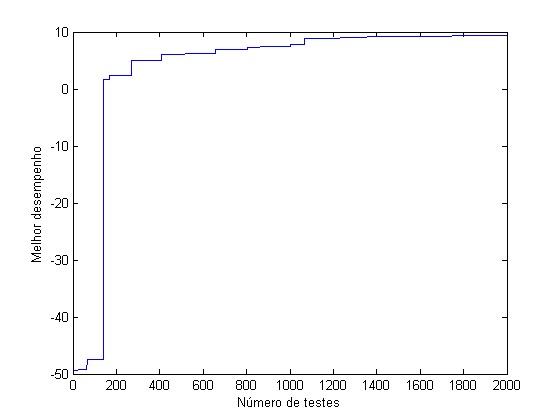
\includegraphics[width=0.6\textwidth]{resultados_otimizacao_3d.png}
  \caption{Resultados da otimiza��o com Modelo Simples e \ac{AG}.}
	\label{fig:convergencia_ag_simples}
\end{figure}

\begin{figure}[ht!]
	\centering
	\setlength\figureheight{0.4\textwidth}
	\setlength\figurewidth{0.7\textwidth}
	% This file was created by matlab2tikz v0.2.3.
% Copyright (c) 2008--2012, Nico Schlömer <nico.schloemer@gmail.com>
% All rights reserved.
% 
% The latest updates can be retrieved from
%   http://www.mathworks.com/matlabcentral/fileexchange/22022-matlab2tikz
% where you can also make suggestions and rate matlab2tikz.
% 
% 
% 
\begin{tikzpicture}

\begin{axis}[%
view={0}{90},
width=4.52083333333333in,
height=3.565625in,
scale only axis,
xmin=0, xmax=1800,
xlabel={N�mero de testes},
ymin=-60, ymax=10,
ylabel={Melhor desempenho}]
\addplot [
color=blue,
solid,
forget plot
]
coordinates{
 (1,-50.0812)(2,-49.7513)(3,-49.7513)(4,-49.7513)(5,-49.7513)(6,-49.3413)(7,-49.3413)(8,-49.3413)(9,-49.3413)(10,-49.3413)(11,-49.3413)(12,-49.3413)(13,-49.3413)(14,-49.3413)(15,-49.3413)(16,-49.3413)(17,-49.3413)(18,-49.3413)(19,-49.3413)(20,-49.3413)(21,-49.3413)(22,-49.3413)(23,-49.3413)(24,-49.3413)(25,-49.3413)(26,-49.3413)(27,-49.3413)(28,-49.3413)(29,-49.3413)(30,-49.3413)(31,-49.3413)(32,-49.3413)(33,-49.3413)(34,-49.3413)(35,-49.3413)(36,-49.3413)(37,-49.3413)(38,-49.3413)(39,-49.3413)(40,-49.3413)(41,-49.3413)(42,-49.3413)(43,-49.3413)(44,-49.3413)(45,-49.3413)(46,-49.3413)(47,-49.3413)(48,-49.3413)(49,-49.3413)(50,-49.3413)(51,-49.3413)(52,-49.3413)(53,-49.3413)(54,-49.3413)(55,-49.3413)(56,-49.3413)(57,-49.3413)(58,-49.3413)(59,2.43137)(60,2.43137)(61,2.43137)(62,2.43137)(63,2.43137)(64,2.89407)(65,2.89407)(66,2.89407)(67,2.89407)(68,2.89407)(69,2.89407)(70,2.89407)(71,2.89407)(72,2.89407)(73,2.89407)(74,2.89407)(75,2.89407)(76,2.89407)(77,2.89407)(78,2.89407)(79,2.89407)(80,2.89407)(81,2.89407)(82,2.89407)(83,2.89407)(84,2.89407)(85,2.89407)(86,2.89407)(87,2.89407)(88,2.89407)(89,2.89407)(90,2.89407)(91,2.89407)(92,2.89407)(93,2.89407)(94,2.89407)(95,2.89407)(96,2.89407)(97,2.89407)(98,2.89407)(99,2.89407)(100,2.89407)(101,2.89407)(102,2.89407)(103,2.89407)(104,2.89407)(105,2.89407)(106,2.89407)(107,2.89407)(108,2.89407)(109,2.89407)(110,2.89407)(111,2.89407)(112,2.89407)(113,2.89407)(114,2.89407)(115,2.89407)(116,2.89407)(117,2.89407)(118,2.89407)(119,2.89407)(120,2.89407)(121,2.89407)(122,2.89407)(123,2.89407)(124,2.89407)(125,2.89407)(126,2.89407)(127,2.89407)(128,2.89407)(129,2.89407)(130,2.89407)(131,2.89407)(132,2.89407)(133,2.89407)(134,2.89407)(135,2.89407)(136,2.89407)(137,2.89407)(138,2.89407)(139,2.89407)(140,2.89407)(141,2.89407)(142,2.89407)(143,3.0947)(144,3.0947)(145,3.0947)(146,3.0947)(147,3.0947)(148,3.0947)(149,3.0947)(150,3.0947)(151,3.0947)(152,3.0947)(153,3.0947)(154,3.0947)(155,3.0947)(156,3.0947)(157,3.0947)(158,3.0947)(159,3.0947)(160,3.0947)(161,3.0947)(162,3.0947)(163,3.0947)(164,3.0947)(165,3.0947)(166,3.0947)(167,3.0947)(168,3.0947)(169,3.0947)(170,3.0947)(171,3.0947)(172,3.0947)(173,3.0947)(174,3.0947)(175,3.0947)(176,3.0947)(177,3.0947)(178,3.0947)(179,3.0947)(180,3.0947)(181,3.0947)(182,3.0947)(183,3.0947)(184,3.0947)(185,3.0947)(186,3.0947)(187,3.0947)(188,3.0947)(189,3.0947)(190,3.0947)(191,3.0947)(192,3.0947)(193,3.0947)(194,3.0947)(195,3.0947)(196,3.0947)(197,3.0947)(198,3.0947)(199,3.0947)(200,3.0947)(201,3.0947)(202,3.0947)(203,3.0947)(204,3.0947)(205,3.0947)(206,3.0947)(207,3.0947)(208,3.0947)(209,3.0947)(210,3.0947)(211,3.0947)(212,3.0947)(213,3.0947)(214,3.0947)(215,3.0947)(216,3.0947)(217,3.0947)(218,3.0947)(219,3.0947)(220,3.0947)(221,3.0947)(222,3.0947)(223,3.0947)(224,3.0947)(225,3.0947)(226,3.0947)(227,3.0947)(228,3.0947)(229,3.0947)(230,3.0947)(231,3.0947)(232,3.0947)(233,3.0947)(234,3.0947)(235,3.0947)(236,3.0947)(237,3.0947)(238,3.0947)(239,3.0947)(240,3.0947)(241,3.0947)(242,3.0947)(243,3.0947)(244,3.0947)(245,3.0947)(246,3.0947)(247,3.0947)(248,3.0947)(249,3.0947)(250,3.0947)(251,3.0947)(252,3.0947)(253,3.0947)(254,3.0947)(255,3.0947)(256,3.0947)(257,3.0947)(258,3.0947)(259,3.0947)(260,3.0947)(261,3.0947)(262,3.0947)(263,3.0947)(264,3.0947)(265,3.0947)(266,3.0947)(267,3.0947)(268,3.0947)(269,3.0947)(270,3.0947)(271,3.0947)(272,3.0947)(273,3.0947)(274,3.0947)(275,3.0947)(276,3.0947)(277,3.0947)(278,3.0947)(279,3.0947)(280,3.0947)(281,3.0947)(282,3.0947)(283,3.0947)(284,3.0947)(285,3.0947)(286,3.0947)(287,3.0947)(288,3.0947)(289,3.0947)(290,3.0947)(291,3.0947)(292,3.0947)(293,3.0947)(294,3.0947)(295,3.0947)(296,3.0947)(297,3.0947)(298,3.0947)(299,3.0947)(300,3.0947)(301,3.0947)(302,3.0947)(303,3.0947)(304,3.0947)(305,3.0947)(306,3.0947)(307,3.0947)(308,3.0947)(309,3.0947)(310,3.0947)(311,3.0947)(312,3.0947)(313,3.0947)(314,3.0947)(315,3.0947)(316,3.0947)(317,3.0947)(318,3.0947)(319,3.0947)(320,3.0947)(321,3.0947)(322,3.0947)(323,3.0947)(324,3.0947)(325,3.0947)(326,3.0947)(327,3.0947)(328,3.0947)(329,3.0947)(330,3.0947)(331,3.0947)(332,3.0947)(333,3.0947)(334,3.0947)(335,3.0947)(336,3.0947)(337,3.0947)(338,3.0947)(339,3.0947)(340,3.0947)(341,3.0947)(342,3.0947)(343,3.0947)(344,3.0947)(345,3.0947)(346,3.0947)(347,3.0947)(348,5.48533)(349,5.48533)(350,5.48533)(351,5.48533)(352,5.48533)(353,5.48533)(354,5.48533)(355,5.48533)(356,5.48533)(357,5.48533)(358,5.48533)(359,5.48533)(360,5.48533)(361,5.48533)(362,5.48533)(363,5.48533)(364,5.48533)(365,5.48533)(366,5.48533)(367,5.48533)(368,5.48533)(369,5.48533)(370,5.48533)(371,5.48533)(372,5.48533)(373,5.48533)(374,5.48533)(375,5.48533)(376,5.48533)(377,5.48533)(378,5.48533)(379,5.48533)(380,5.48533)(381,5.48533)(382,5.48533)(383,5.48533)(384,5.48533)(385,5.48533)(386,5.48533)(387,5.48533)(388,5.48533)(389,5.48533)(390,5.48533)(391,5.48533)(392,5.48533)(393,5.48533)(394,5.48533)(395,5.48533)(396,5.48533)(397,5.48533)(398,5.48533)(399,5.48533)(400,5.48533)(401,5.48533)(402,5.48533)(403,5.48533)(404,5.48533)(405,5.48533)(406,5.48533)(407,5.48533)(408,5.48533)(409,5.48533)(410,5.48533)(411,5.48533)(412,5.48533)(413,5.48533)(414,5.48533)(415,5.48533)(416,5.48533)(417,5.48533)(418,5.48533)(419,5.48533)(420,5.48533)(421,5.48533)(422,5.48533)(423,5.48533)(424,5.48533)(425,5.48533)(426,5.48533)(427,5.48533)(428,5.48533)(429,5.48533)(430,5.48533)(431,5.48533)(432,5.48533)(433,5.48533)(434,5.48533)(435,5.48533)(436,5.48533)(437,5.48533)(438,5.48533)(439,5.48533)(440,5.48533)(441,5.48533)(442,5.48533)(443,5.48533)(444,5.48533)(445,5.48533)(446,5.48533)(447,5.48533)(448,5.48533)(449,5.48533)(450,5.48533)(451,5.48533)(452,5.48533)(453,5.48533)(454,5.48533)(455,5.48533)(456,5.48533)(457,5.48533)(458,5.48533)(459,5.48533)(460,5.48533)(461,5.48533)(462,5.48533)(463,5.48533)(464,5.48533)(465,5.48533)(466,5.48533)(467,5.48533)(468,5.48533)(469,5.48533)(470,5.48533)(471,5.48533)(472,5.48533)(473,5.48533)(474,5.48533)(475,5.48533)(476,5.48533)(477,8.30803)(478,8.30803)(479,8.30803)(480,8.30803)(481,8.30803)(482,8.30803)(483,8.30803)(484,8.30803)(485,8.30803)(486,8.30803)(487,8.30803)(488,8.30803)(489,8.30803)(490,8.30803)(491,8.30803)(492,8.30803)(493,8.30803)(494,8.30803)(495,8.30803)(496,8.30803)(497,8.30803)(498,8.30803)(499,8.30803)(500,8.30803)(501,8.30803)(502,8.30803)(503,8.30803)(504,8.30803)(505,8.30803)(506,8.30803)(507,8.30803)(508,8.30803)(509,8.30803)(510,8.30803)(511,8.30803)(512,8.30803)(513,8.30803)(514,8.30803)(515,8.30803)(516,8.30803)(517,8.30803)(518,8.30803)(519,8.30803)(520,8.30803)(521,8.30803)(522,8.30803)(523,8.30803)(524,8.30803)(525,8.30803)(526,8.30803)(527,8.30803)(528,8.30803)(529,8.30803)(530,8.30803)(531,8.30803)(532,8.30803)(533,8.30803)(534,8.30803)(535,8.30803)(536,8.30803)(537,8.30803)(538,8.30803)(539,8.30803)(540,8.30803)(541,8.30803)(542,8.30803)(543,8.30803)(544,8.30803)(545,8.30803)(546,8.30803)(547,8.30803)(548,8.30803)(549,8.30803)(550,8.30803)(551,8.30803)(552,8.30803)(553,8.30803)(554,8.30803)(555,8.30803)(556,8.30803)(557,8.30803)(558,8.30803)(559,8.30803)(560,8.30803)(561,8.30803)(562,8.30803)(563,8.30803)(564,8.30803)(565,8.30803)(566,8.30803)(567,8.30803)(568,8.30803)(569,8.30803)(570,8.30803)(571,8.30803)(572,8.30803)(573,8.30803)(574,8.30803)(575,8.30803)(576,8.30803)(577,8.30803)(578,8.30803)(579,8.30803)(580,8.30803)(581,8.30803)(582,8.30803)(583,8.30803)(584,8.30803)(585,8.30803)(586,8.30803)(587,8.30803)(588,8.30803)(589,8.30803)(590,8.30803)(591,8.30803)(592,8.30803)(593,8.30803)(594,8.30803)(595,8.30803)(596,8.30803)(597,8.30803)(598,8.30803)(599,8.30803)(600,8.30803)(601,8.30803)(602,8.30803)(603,8.30803)(604,8.30803)(605,8.30803)(606,8.30803)(607,8.30803)(608,8.30803)(609,8.30803)(610,8.30803)(611,8.30803)(612,8.30803)(613,8.30803)(614,8.30803)(615,8.30803)(616,8.30803)(617,8.30803)(618,8.30803)(619,8.30803)(620,8.30803)(621,8.30803)(622,8.30803)(623,8.30803)(624,8.30803)(625,8.30803)(626,8.30803)(627,8.30803)(628,8.30803)(629,8.30803)(630,8.30803)(631,8.30803)(632,8.30803)(633,8.30803)(634,8.30803)(635,8.30803)(636,8.30803)(637,8.30803)(638,8.30803)(639,8.30803)(640,8.30803)(641,8.30803)(642,8.30803)(643,8.30803)(644,8.30803)(645,8.30803)(646,8.30803)(647,8.30803)(648,8.30803)(649,8.30803)(650,8.30803)(651,8.30803)(652,8.30803)(653,8.30803)(654,8.30803)(655,8.30803)(656,8.30803)(657,8.30803)(658,8.30803)(659,8.30803)(660,8.30803)(661,8.30803)(662,8.30803)(663,8.30803)(664,8.30803)(665,8.30803)(666,8.30803)(667,8.30803)(668,8.30803)(669,8.30803)(670,8.30803)(671,8.30803)(672,8.30803)(673,8.30803)(674,8.30803)(675,8.30803)(676,8.30803)(677,8.30803)(678,8.30803)(679,8.30803)(680,8.30803)(681,8.30803)(682,8.30803)(683,8.30803)(684,8.30803)(685,8.30803)(686,8.30803)(687,8.30803)(688,8.30803)(689,8.30803)(690,8.30803)(691,8.30803)(692,8.30803)(693,8.30803)(694,8.30803)(695,8.30803)(696,8.30803)(697,8.30803)(698,8.30803)(699,8.30803)(700,8.30803)(701,8.30803)(702,8.30803)(703,8.30803)(704,8.30803)(705,8.30803)(706,8.30803)(707,8.30803)(708,8.30803)(709,8.30803)(710,8.30803)(711,8.30803)(712,8.30803)(713,8.30803)(714,8.30803)(715,8.30803)(716,8.30803)(717,8.30803)(718,8.30803)(719,8.30803)(720,8.30803)(721,8.30803)(722,8.30803)(723,8.30803)(724,8.30803)(725,8.30803)(726,8.30803)(727,8.30803)(728,8.30803)(729,8.30803)(730,8.30803)(731,8.30803)(732,8.30803)(733,8.30803)(734,8.30803)(735,8.30803)(736,8.30803)(737,8.30803)(738,8.30803)(739,8.30803)(740,8.30803)(741,8.30803)(742,8.30803)(743,8.30803)(744,8.30803)(745,8.30803)(746,8.30803)(747,8.30803)(748,8.30803)(749,8.30803)(750,8.30803)(751,8.30803)(752,8.30803)(753,8.30803)(754,8.30803)(755,8.30803)(756,8.30803)(757,8.30803)(758,8.30803)(759,8.30803)(760,8.30803)(761,8.30803)(762,8.30803)(763,8.30803)(764,8.30803)(765,8.30803)(766,8.30803)(767,8.30803)(768,8.30803)(769,8.30803)(770,8.30803)(771,8.30803)(772,8.30803)(773,8.30803)(774,8.30803)(775,8.30803)(776,8.30803)(777,8.30803)(778,8.30803)(779,8.30803)(780,8.30803)(781,8.30803)(782,8.30803)(783,8.30803)(784,8.30803)(785,8.30803)(786,8.30803)(787,8.30803)(788,8.30803)(789,8.30803)(790,8.30803)(791,8.30803)(792,8.30803)(793,8.30803)(794,8.30803)(795,8.30803)(796,8.30803)(797,8.30803)(798,8.30803)(799,8.30803)(800,8.30803)(801,8.30803)(802,8.30803)(803,8.30803)(804,8.30803)(805,8.30803)(806,8.30803)(807,8.30803)(808,8.30803)(809,8.30803)(810,8.30803)(811,8.30803)(812,8.30803)(813,8.30803)(814,8.30803)(815,8.30803)(816,8.30803)(817,8.30803)(818,8.30803)(819,8.30803)(820,8.30803)(821,8.30803)(822,8.30803)(823,8.30803)(824,8.30803)(825,8.30803)(826,8.30803)(827,8.30803)(828,8.30803)(829,8.30803)(830,8.30803)(831,8.30803)(832,8.30803)(833,8.30803)(834,8.30803)(835,8.30803)(836,8.30803)(837,8.30803)(838,8.30803)(839,8.30803)(840,8.30803)(841,8.30803)(842,8.30803)(843,8.30803)(844,8.30803)(845,8.30803)(846,8.30803)(847,8.30803)(848,8.30803)(849,8.30803)(850,8.30803)(851,8.30803)(852,8.30803)(853,8.30803)(854,8.30803)(855,8.30803)(856,8.30803)(857,8.30803)(858,8.30803)(859,8.30803)(860,8.30803)(861,8.30803)(862,8.30803)(863,8.30803)(864,8.30803)(865,8.30803)(866,8.30803)(867,8.30803)(868,8.30803)(869,8.30803)(870,8.30803)(871,8.30803)(872,8.30803)(873,8.30803)(874,8.30803)(875,8.30803)(876,8.30803)(877,8.30803)(878,8.30803)(879,8.30803)(880,8.30803)(881,8.30803)(882,8.30803)(883,8.30803)(884,8.30803)(885,8.30803)(886,8.30803)(887,8.30803)(888,8.30803)(889,8.30803)(890,8.30803)(891,8.30803)(892,8.30803)(893,8.30803)(894,8.30803)(895,8.30803)(896,8.30803)(897,8.30803)(898,8.30803)(899,8.30803)(900,8.30803)(901,8.30803)(902,8.30803)(903,8.30803)(904,8.30803)(905,8.30803)(906,8.30803)(907,8.30803)(908,8.30803)(909,8.30803)(910,8.30803)(911,8.30803)(912,8.30803)(913,8.30803)(914,8.30803)(915,8.30803)(916,8.30803)(917,8.30803)(918,8.30803)(919,8.30803)(920,8.30803)(921,8.30803)(922,8.30803)(923,8.30803)(924,8.30803)(925,8.30803)(926,8.30803)(927,8.30803)(928,8.30803)(929,8.30803)(930,8.30803)(931,8.30803)(932,8.30803)(933,8.30803)(934,8.30803)(935,8.30803)(936,8.30803)(937,8.30803)(938,8.30803)(939,8.30803)(940,8.30803)(941,8.30803)(942,8.30803)(943,8.30803)(944,8.30803)(945,8.30803)(946,8.30803)(947,8.30803)(948,8.30803)(949,8.30803)(950,8.30803)(951,8.30803)(952,8.30803)(953,8.30803)(954,8.30803)(955,8.30803)(956,8.30803)(957,8.30803)(958,8.30803)(959,8.30803)(960,8.30803)(961,8.30803)(962,8.30803)(963,8.30803)(964,8.30803)(965,8.30803)(966,8.30803)(967,8.30803)(968,8.30803)(969,8.30803)(970,8.30803)(971,8.30803)(972,8.30803)(973,8.30803)(974,8.30803)(975,8.30803)(976,8.30803)(977,8.30803)(978,8.30803)(979,8.30803)(980,8.30803)(981,8.30803)(982,8.30803)(983,8.30803)(984,8.30803)(985,8.30803)(986,8.30803)(987,8.30803)(988,8.30803)(989,8.30803)(990,8.30803)(991,8.30803)(992,8.30803)(993,8.30803)(994,8.30803)(995,8.30803)(996,8.30803)(997,8.30803)(998,8.30803)(999,8.30803)(1000,8.30803)(1001,8.30803)(1002,8.30803)(1003,8.30803)(1004,8.30803)(1005,8.30803)(1006,8.30803)(1007,8.30803)(1008,8.30803)(1009,8.30803)(1010,8.30803)(1011,8.30803)(1012,8.30803)(1013,8.30803)(1014,8.30803)(1015,8.30803)(1016,8.30803)(1017,8.30803)(1018,8.30803)(1019,8.30803)(1020,8.30803)(1021,8.30803)(1022,8.30803)(1023,8.30803)(1024,8.30803)(1025,8.30803)(1026,8.30803)(1027,8.30803)(1028,8.30803)(1029,8.30803)(1030,8.30803)(1031,8.30803)(1032,8.30803)(1033,8.30803)(1034,8.30803)(1035,8.30803)(1036,8.30803)(1037,8.30803)(1038,8.30803)(1039,8.30803)(1040,8.30803)(1041,8.30803)(1042,8.30803)(1043,8.30803)(1044,8.30803)(1045,8.30803)(1046,8.30803)(1047,8.30803)(1048,8.30803)(1049,8.30803)(1050,8.30803)(1051,8.30803)(1052,8.30803)(1053,8.30803)(1054,8.30803)(1055,8.30803)(1056,8.30803)(1057,8.30803)(1058,8.30803)(1059,8.30803)(1060,8.30803)(1061,8.30803)(1062,8.30803)(1063,8.30803)(1064,8.30803)(1065,8.30803)(1066,8.30803)(1067,8.30803)(1068,8.30803)(1069,8.30803)(1070,8.30803)(1071,8.30803)(1072,8.30803)(1073,8.30803)(1074,8.30803)(1075,8.30803)(1076,8.30803)(1077,8.30803)(1078,8.30803)(1079,8.30803)(1080,8.30803)(1081,8.30803)(1082,8.30803)(1083,8.30803)(1084,8.30803)(1085,8.30803)(1086,8.30803)(1087,8.30803)(1088,8.30803)(1089,8.30803)(1090,8.30803)(1091,8.30803)(1092,8.30803)(1093,8.30803)(1094,8.30803)(1095,8.30803)(1096,8.30803)(1097,8.30803)(1098,8.30803)(1099,8.30803)(1100,8.30803)(1101,8.30803)(1102,8.30803)(1103,8.30803)(1104,8.30803)(1105,8.30803)(1106,8.30803)(1107,8.30803)(1108,8.30803)(1109,8.30803)(1110,8.30803)(1111,8.30803)(1112,8.30803)(1113,8.30803)(1114,8.30803)(1115,8.30803)(1116,8.30803)(1117,8.30803)(1118,8.30803)(1119,8.30803)(1120,8.30803)(1121,8.30803)(1122,8.30803)(1123,8.30803)(1124,8.30803)(1125,8.30803)(1126,8.30803)(1127,8.30803)(1128,8.30803)(1129,8.30803)(1130,8.30803)(1131,8.30803)(1132,8.30803)(1133,8.30803)(1134,8.30803)(1135,8.30803)(1136,8.30803)(1137,8.30803)(1138,8.30803)(1139,8.30803)(1140,8.30803)(1141,8.30803)(1142,8.30803)(1143,8.30803)(1144,8.30803)(1145,8.30803)(1146,8.30803)(1147,8.30803)(1148,8.30803)(1149,8.30803)(1150,8.30803)(1151,8.30803)(1152,8.30803)(1153,8.30803)(1154,8.30803)(1155,8.30803)(1156,8.30803)(1157,8.30803)(1158,8.30803)(1159,8.30803)(1160,8.30803)(1161,8.30803)(1162,8.30803)(1163,8.30803)(1164,8.30803)(1165,8.30803)(1166,8.30803)(1167,8.30803)(1168,8.30803)(1169,8.30803)(1170,8.30803)(1171,8.30803)(1172,8.30803)(1173,8.30803)(1174,8.30803)(1175,8.30803)(1176,8.30803)(1177,8.30803)(1178,8.30803)(1179,8.30803)(1180,8.30803)(1181,8.30803)(1182,8.30803)(1183,8.30803)(1184,8.30803)(1185,8.30803)(1186,8.30803)(1187,8.30803)(1188,8.30803)(1189,8.30803)(1190,8.30803)(1191,8.30803)(1192,8.30803)(1193,8.30803)(1194,8.30803)(1195,8.30803)(1196,8.30803)(1197,8.30803)(1198,8.30803)(1199,8.30803)(1200,8.30803)(1201,8.30803)(1202,8.30803)(1203,8.30803)(1204,8.30803)(1205,8.30803)(1206,8.30803)(1207,8.30803)(1208,8.30803)(1209,8.30803)(1210,8.30803)(1211,8.30803)(1212,8.30803)(1213,8.30803)(1214,8.30803)(1215,8.30803)(1216,8.30803)(1217,8.30803)(1218,8.30803)(1219,8.30803)(1220,8.30803)(1221,8.30803)(1222,8.30803)(1223,8.30803)(1224,8.30803)(1225,8.30803)(1226,8.30803)(1227,8.30803)(1228,8.30803)(1229,8.30803)(1230,8.30803)(1231,8.30803)(1232,8.30803)(1233,8.30803)(1234,8.30803)(1235,8.30803)(1236,8.30803)(1237,8.30803)(1238,8.30803)(1239,8.30803)(1240,8.30803)(1241,8.30803)(1242,8.30803)(1243,8.30803)(1244,8.30803)(1245,8.30803)(1246,8.30803)(1247,8.30803)(1248,8.30803)(1249,8.30803)(1250,8.30803)(1251,8.30803)(1252,8.30803)(1253,8.30803)(1254,8.30803)(1255,8.30803)(1256,8.30803)(1257,8.30803)(1258,8.30803)(1259,8.30803)(1260,8.30803)(1261,8.30803)(1262,8.30803)(1263,8.30803)(1264,8.30803)(1265,8.30803)(1266,8.30803)(1267,8.30803)(1268,8.30803)(1269,8.30803)(1270,8.30803)(1271,8.30803)(1272,8.30803)(1273,8.30803)(1274,8.30803)(1275,8.30803)(1276,8.30803)(1277,8.30803)(1278,8.30803)(1279,8.30803)(1280,8.30803)(1281,8.30803)(1282,8.30803)(1283,8.30803)(1284,8.30803)(1285,8.30803)(1286,8.30803)(1287,8.30803)(1288,8.30803)(1289,8.30803)(1290,8.30803)(1291,8.30803)(1292,8.30803)(1293,8.30803)(1294,8.30803)(1295,8.30803)(1296,8.30803)(1297,8.30803)(1298,8.30803)(1299,8.30803)(1300,8.30803)(1301,8.30803)(1302,8.30803)(1303,8.30803)(1304,8.30803)(1305,8.30803)(1306,8.30803)(1307,8.30803)(1308,8.30803)(1309,8.30803)(1310,8.30803)(1311,8.30803)(1312,8.30803)(1313,8.30803)(1314,8.30803)(1315,8.30803)(1316,8.30803)(1317,8.30803)(1318,8.30803)(1319,8.30803)(1320,8.30803)(1321,8.30803)(1322,8.30803)(1323,8.30803)(1324,8.30803)(1325,8.30803)(1326,8.30803)(1327,8.30803)(1328,8.30803)(1329,8.30803)(1330,8.30803)(1331,8.30803)(1332,8.30803)(1333,8.30803)(1334,8.30803)(1335,8.30803)(1336,8.30803)(1337,8.30803)(1338,8.30803)(1339,8.30803)(1340,8.30803)(1341,8.30803)(1342,8.30803)(1343,8.30803)(1344,8.30803)(1345,8.30803)(1346,8.30803)(1347,8.30803)(1348,8.30803)(1349,8.30803)(1350,8.30803)(1351,8.30803)(1352,8.30803)(1353,8.30803)(1354,8.30803)(1355,8.30803)(1356,8.30803)(1357,8.30803)(1358,8.30803)(1359,8.30803)(1360,8.30803)(1361,8.30803)(1362,8.30803)(1363,8.30803)(1364,8.30803)(1365,8.30803)(1366,8.30803)(1367,8.30803)(1368,8.30803)(1369,8.30803)(1370,8.30803)(1371,8.30803)(1372,8.30803)(1373,8.30803)(1374,8.30803)(1375,8.30803)(1376,8.30803)(1377,8.30803)(1378,8.30803)(1379,8.30803)(1380,8.30803)(1381,8.30803)(1382,8.30803)(1383,8.30803)(1384,8.30803)(1385,8.30803)(1386,8.30803)(1387,8.30803)(1388,8.30803)(1389,8.30803)(1390,8.30803)(1391,8.30803)(1392,8.30803)(1393,8.30803)(1394,8.30803)(1395,8.30803)(1396,8.30803)(1397,8.30803)(1398,8.30803)(1399,8.30803)(1400,8.30803)(1401,8.30803)(1402,8.30803)(1403,8.30803)(1404,8.30803)(1405,8.30803)(1406,8.30803)(1407,8.30803)(1408,8.30803)(1409,8.30803)(1410,8.30803)(1411,8.30803)(1412,8.30803)(1413,8.30803)(1414,8.30803)(1415,8.30803)(1416,8.30803)(1417,8.30803)(1418,8.30803)(1419,8.30803)(1420,8.30803)(1421,8.30803)(1422,8.30803)(1423,8.30803)(1424,8.30803)(1425,8.30803)(1426,8.30803)(1427,8.30803)(1428,8.30803)(1429,8.30803)(1430,8.30803)(1431,8.30803)(1432,8.30803)(1433,8.30803)(1434,8.30803)(1435,8.30803)(1436,8.30803)(1437,8.30803)(1438,8.30803)(1439,8.30803)(1440,8.30803)(1441,8.30803)(1442,8.30803)(1443,8.30803)(1444,8.30803)(1445,8.30803)(1446,8.30803)(1447,8.30803)(1448,8.30803)(1449,8.30803)(1450,8.30803)(1451,8.30803)(1452,8.30803)(1453,8.30803)(1454,8.30803)(1455,8.30803)(1456,8.30803)(1457,8.30803)(1458,8.30803)(1459,8.30803)(1460,8.30803)(1461,8.30803)(1462,8.30803)(1463,8.30803)(1464,8.30803)(1465,8.30803)(1466,8.30803)(1467,8.30803)(1468,8.30803)(1469,8.30803)(1470,8.30803)(1471,8.30803)(1472,8.30803)(1473,8.30803)(1474,8.30803)(1475,8.30803)(1476,8.30803)(1477,8.30803)(1478,8.30803)(1479,8.30803)(1480,8.30803)(1481,8.30803)(1482,8.30803)(1483,8.30803)(1484,8.30803)(1485,8.30803)(1486,8.30803)(1487,8.30803)(1488,8.30803)(1489,8.30803)(1490,8.30803)(1491,8.30803)(1492,8.30803)(1493,8.30803)(1494,8.30803)(1495,8.30803)(1496,8.30803)(1497,8.30803)(1498,8.30803)(1499,8.30803)(1500,8.30803)(1501,8.30803)(1502,8.30803)(1503,8.30803)(1504,8.30803)(1505,8.30803)(1506,8.30803)(1507,8.30803)(1508,8.30803)(1509,8.30803)(1510,8.30803)(1511,8.30803)(1512,8.30803)(1513,8.30803)(1514,8.30803)(1515,8.30803)(1516,8.30803)(1517,8.30803)(1518,8.30803)(1519,8.30803)(1520,8.30803)(1521,8.30803)(1522,8.30803)(1523,8.30803)(1524,8.30803)(1525,8.30803)(1526,8.30803)(1527,8.30803)(1528,8.30803)(1529,8.30803)(1530,8.30803)(1531,8.30803)(1532,8.30803)(1533,8.30803)(1534,8.30803)(1535,8.30803)(1536,8.30803)(1537,8.30803)(1538,8.30803)(1539,8.30803)(1540,8.30803)(1541,8.30803)(1542,8.30803)(1543,8.30803)(1544,8.30803)(1545,8.30803)(1546,8.30803)(1547,8.30803)(1548,8.30803)(1549,8.30803)(1550,8.30803)(1551,8.30803)(1552,8.30803)(1553,8.30803)(1554,8.30803)(1555,8.30803)(1556,8.30803)(1557,8.30803)(1558,8.30803)(1559,8.30803)(1560,8.30803)(1561,8.30803)(1562,8.30803)(1563,8.30803)(1564,8.30803)(1565,8.30803)(1566,8.30803)(1567,8.30803)(1568,8.30803)(1569,8.30803)(1570,8.30803)(1571,8.30803)(1572,8.30803)(1573,8.30803)(1574,8.30803)(1575,8.30803)(1576,8.30803)(1577,8.30803)(1578,8.30803)(1579,8.30803)(1580,8.30803)(1581,8.30803)(1582,8.30803)(1583,8.30803)(1584,8.30803)(1585,8.30803)(1586,8.30803)(1587,8.30803)(1588,8.30803)(1589,8.30803)(1590,8.30803)(1591,8.30803)(1592,8.30803)(1593,8.30803)(1594,8.30803)(1595,8.30803)(1596,8.30803)(1597,8.30803)(1598,8.30803)(1599,8.30803)(1600,8.30803)(1601,8.30803)(1602,8.30803)(1603,8.30803)(1604,8.30803)(1605,8.30803)(1606,8.30803)(1607,8.30803)(1608,8.30803)(1609,8.30803)(1610,8.30803)(1611,8.30803)(1612,8.30803)(1613,8.30803)(1614,8.30803)(1615,8.30803)(1616,8.30803)(1617,8.30803)(1618,8.30803)(1619,8.30803)(1620,8.30803)(1621,8.30803)(1622,8.30803)(1623,8.30803)(1624,8.30803)(1625,8.30803)(1626,8.30803)(1627,8.30803)(1628,8.30803)(1629,8.30803)(1630,8.30803)(1631,8.30803)(1632,8.30803)(1633,8.30803)(1634,8.30803)(1635,8.30803)(1636,8.30803)(1637,8.30803)(1638,8.30803)(1639,8.30803)(1640,8.30803)(1641,8.30803)(1642,8.30803)(1643,8.30803)(1644,8.30803)(1645,8.30803)(1646,8.30803)(1647,8.30803)(1648,8.30803)(1649,8.30803)(1650,8.30803)(1651,8.30803)(1652,8.30803)(1653,8.30803)(1654,8.30803)(1655,8.30803)(1656,8.30803)(1657,8.30803)(1658,8.30803)(1659,8.30803)(1660,8.30803)(1661,8.30803)(1662,8.30803)(1663,8.30803)(1664,8.30803)(1665,8.30803)(1666,8.30803)(1667,8.30803)(1668,8.30803)(1669,8.30803)(1670,8.30803)(1671,8.30803)(1672,8.30803)(1673,8.30803)(1674,8.30803)(1675,8.30803)(1676,8.30803)(1677,8.30803)(1678,8.30803) 
};
\end{axis}
\end{tikzpicture}%
		%\includegraphics[width=0.6\textwidth]{resultados_otimizacao_3d.png}
  \caption{Resultados da otimiza��o com Modelo com Movimento de Bra�os e \ac{AG}.}
	\label{fig:convergencia_ag_bracos}
\end{figure}

\begin{figure}[ht!]
	\centering
	\setlength\figureheight{0.4\textwidth}
	\setlength\figurewidth{0.7\textwidth}
	% This file was created by matlab2tikz v0.2.3.
% Copyright (c) 2008--2012, Nico Schlömer <nico.schloemer@gmail.com>
% All rights reserved.
% 
% The latest updates can be retrieved from
%   http://www.mathworks.com/matlabcentral/fileexchange/22022-matlab2tikz
% where you can also make suggestions and rate matlab2tikz.
% 
% 
% 
\begin{tikzpicture}

\begin{axis}[%
view={0}{90},
width=4.52083333333333in,
height=3.565625in,
scale only axis,
xmin=0, xmax=1800,
xlabel={N�mero de testes},
ymin=-60, ymax=10,
ylabel={Melhor desempenho}]
\addplot [
color=blue,
solid,
forget plot
]
coordinates{
 (1,-50.0812)(2,-49.7513)(3,-49.7513)(4,-49.7513)(5,-49.7513)(6,-49.3413)(7,-49.3413)(8,-49.3413)(9,-49.3413)(10,-49.3413)(11,-49.3413)(12,-49.3413)(13,-49.3413)(14,-49.3413)(15,-49.3413)(16,-49.3413)(17,-49.3413)(18,-49.3413)(19,-49.3413)(20,-49.3413)(21,-49.3413)(22,-49.3413)(23,-49.3413)(24,-49.3413)(25,-49.3413)(26,-49.3413)(27,-49.3413)(28,-49.3413)(29,-49.3413)(30,-49.3413)(31,-49.3413)(32,-49.3413)(33,-49.3413)(34,-49.3413)(35,-49.3413)(36,-49.3413)(37,-49.3413)(38,-49.3413)(39,-49.3413)(40,-49.3413)(41,-49.3413)(42,-49.3413)(43,-49.3413)(44,-49.3413)(45,-49.3413)(46,-49.3413)(47,-49.3413)(48,-49.3413)(49,-49.3413)(50,-49.3413)(51,-49.3413)(52,-49.3413)(53,-49.3413)(54,-49.3413)(55,-49.3413)(56,-49.3413)(57,-49.3413)(58,-49.3413)(59,2.43137)(60,2.43137)(61,2.43137)(62,2.43137)(63,2.43137)(64,2.89407)(65,2.89407)(66,2.89407)(67,2.89407)(68,2.89407)(69,2.89407)(70,2.89407)(71,2.89407)(72,2.89407)(73,2.89407)(74,2.89407)(75,2.89407)(76,2.89407)(77,2.89407)(78,2.89407)(79,2.89407)(80,2.89407)(81,2.89407)(82,2.89407)(83,2.89407)(84,2.89407)(85,2.89407)(86,2.89407)(87,2.89407)(88,2.89407)(89,2.89407)(90,2.89407)(91,2.89407)(92,2.89407)(93,2.89407)(94,2.89407)(95,2.89407)(96,2.89407)(97,2.89407)(98,2.89407)(99,2.89407)(100,2.89407)(101,2.89407)(102,2.89407)(103,2.89407)(104,2.89407)(105,2.89407)(106,2.89407)(107,2.89407)(108,2.89407)(109,2.89407)(110,2.89407)(111,2.89407)(112,2.89407)(113,2.89407)(114,2.89407)(115,2.89407)(116,2.89407)(117,2.89407)(118,2.89407)(119,2.89407)(120,2.89407)(121,2.89407)(122,2.89407)(123,2.89407)(124,2.89407)(125,2.89407)(126,2.89407)(127,2.89407)(128,2.89407)(129,2.89407)(130,2.89407)(131,2.89407)(132,2.89407)(133,2.89407)(134,2.89407)(135,2.89407)(136,2.89407)(137,2.89407)(138,2.89407)(139,2.89407)(140,2.89407)(141,2.89407)(142,2.89407)(143,3.0947)(144,3.0947)(145,3.0947)(146,3.0947)(147,3.0947)(148,3.0947)(149,3.0947)(150,3.0947)(151,3.0947)(152,3.0947)(153,3.0947)(154,3.0947)(155,3.0947)(156,3.0947)(157,3.0947)(158,3.0947)(159,3.0947)(160,3.0947)(161,3.0947)(162,3.0947)(163,3.0947)(164,3.0947)(165,3.0947)(166,3.0947)(167,3.0947)(168,3.0947)(169,3.0947)(170,3.0947)(171,3.0947)(172,3.0947)(173,3.0947)(174,3.0947)(175,3.0947)(176,3.0947)(177,3.0947)(178,3.0947)(179,3.0947)(180,3.0947)(181,3.0947)(182,3.0947)(183,3.0947)(184,3.0947)(185,3.0947)(186,3.0947)(187,3.0947)(188,3.0947)(189,3.0947)(190,3.0947)(191,3.0947)(192,3.0947)(193,3.0947)(194,3.0947)(195,3.0947)(196,3.0947)(197,3.0947)(198,3.0947)(199,3.0947)(200,3.0947)(201,3.0947)(202,3.0947)(203,3.0947)(204,3.0947)(205,3.0947)(206,3.0947)(207,3.0947)(208,3.0947)(209,3.0947)(210,3.0947)(211,3.0947)(212,3.0947)(213,3.0947)(214,3.0947)(215,3.0947)(216,3.0947)(217,3.0947)(218,3.0947)(219,3.0947)(220,3.0947)(221,3.0947)(222,3.0947)(223,3.0947)(224,3.0947)(225,3.0947)(226,3.0947)(227,3.0947)(228,3.0947)(229,3.0947)(230,3.0947)(231,3.0947)(232,3.0947)(233,3.0947)(234,3.0947)(235,3.0947)(236,3.0947)(237,3.0947)(238,3.0947)(239,3.0947)(240,3.0947)(241,3.0947)(242,3.0947)(243,3.0947)(244,3.0947)(245,3.0947)(246,3.0947)(247,3.0947)(248,3.0947)(249,3.0947)(250,3.0947)(251,3.0947)(252,3.0947)(253,3.0947)(254,3.0947)(255,3.0947)(256,3.0947)(257,3.0947)(258,3.0947)(259,3.0947)(260,3.0947)(261,3.0947)(262,3.0947)(263,3.0947)(264,3.0947)(265,3.0947)(266,3.0947)(267,3.0947)(268,3.0947)(269,3.0947)(270,3.0947)(271,3.0947)(272,3.0947)(273,3.0947)(274,3.0947)(275,3.0947)(276,3.0947)(277,3.0947)(278,3.0947)(279,3.0947)(280,3.0947)(281,3.0947)(282,3.0947)(283,3.0947)(284,3.0947)(285,3.0947)(286,3.0947)(287,3.0947)(288,3.0947)(289,3.0947)(290,3.0947)(291,3.0947)(292,3.0947)(293,3.0947)(294,3.0947)(295,3.0947)(296,3.0947)(297,3.0947)(298,3.0947)(299,3.0947)(300,3.0947)(301,3.0947)(302,3.0947)(303,3.0947)(304,3.0947)(305,3.0947)(306,3.0947)(307,3.0947)(308,3.0947)(309,3.0947)(310,3.0947)(311,3.0947)(312,3.0947)(313,3.0947)(314,3.0947)(315,3.0947)(316,3.0947)(317,3.0947)(318,3.0947)(319,3.0947)(320,3.0947)(321,3.0947)(322,3.0947)(323,3.0947)(324,3.0947)(325,3.0947)(326,3.0947)(327,3.0947)(328,3.0947)(329,3.0947)(330,3.0947)(331,3.0947)(332,3.0947)(333,3.0947)(334,3.0947)(335,3.0947)(336,3.0947)(337,3.0947)(338,3.0947)(339,3.0947)(340,3.0947)(341,3.0947)(342,3.0947)(343,3.0947)(344,3.0947)(345,3.0947)(346,3.0947)(347,3.0947)(348,5.48533)(349,5.48533)(350,5.48533)(351,5.48533)(352,5.48533)(353,5.48533)(354,5.48533)(355,5.48533)(356,5.48533)(357,5.48533)(358,5.48533)(359,5.48533)(360,5.48533)(361,5.48533)(362,5.48533)(363,5.48533)(364,5.48533)(365,5.48533)(366,5.48533)(367,5.48533)(368,5.48533)(369,5.48533)(370,5.48533)(371,5.48533)(372,5.48533)(373,5.48533)(374,5.48533)(375,5.48533)(376,5.48533)(377,5.48533)(378,5.48533)(379,5.48533)(380,5.48533)(381,5.48533)(382,5.48533)(383,5.48533)(384,5.48533)(385,5.48533)(386,5.48533)(387,5.48533)(388,5.48533)(389,5.48533)(390,5.48533)(391,5.48533)(392,5.48533)(393,5.48533)(394,5.48533)(395,5.48533)(396,5.48533)(397,5.48533)(398,5.48533)(399,5.48533)(400,5.48533)(401,5.48533)(402,5.48533)(403,5.48533)(404,5.48533)(405,5.48533)(406,5.48533)(407,5.48533)(408,5.48533)(409,5.48533)(410,5.48533)(411,5.48533)(412,5.48533)(413,5.48533)(414,5.48533)(415,5.48533)(416,5.48533)(417,5.48533)(418,5.48533)(419,5.48533)(420,5.48533)(421,5.48533)(422,5.48533)(423,5.48533)(424,5.48533)(425,5.48533)(426,5.48533)(427,5.48533)(428,5.48533)(429,5.48533)(430,5.48533)(431,5.48533)(432,5.48533)(433,5.48533)(434,5.48533)(435,5.48533)(436,5.48533)(437,5.48533)(438,5.48533)(439,5.48533)(440,5.48533)(441,5.48533)(442,5.48533)(443,5.48533)(444,5.48533)(445,5.48533)(446,5.48533)(447,5.48533)(448,5.48533)(449,5.48533)(450,5.48533)(451,5.48533)(452,5.48533)(453,5.48533)(454,5.48533)(455,5.48533)(456,5.48533)(457,5.48533)(458,5.48533)(459,5.48533)(460,5.48533)(461,5.48533)(462,5.48533)(463,5.48533)(464,5.48533)(465,5.48533)(466,5.48533)(467,5.48533)(468,5.48533)(469,5.48533)(470,5.48533)(471,5.48533)(472,5.48533)(473,5.48533)(474,5.48533)(475,5.48533)(476,5.48533)(477,8.30803)(478,8.30803)(479,8.30803)(480,8.30803)(481,8.30803)(482,8.30803)(483,8.30803)(484,8.30803)(485,8.30803)(486,8.30803)(487,8.30803)(488,8.30803)(489,8.30803)(490,8.30803)(491,8.30803)(492,8.30803)(493,8.30803)(494,8.30803)(495,8.30803)(496,8.30803)(497,8.30803)(498,8.30803)(499,8.30803)(500,8.30803)(501,8.30803)(502,8.30803)(503,8.30803)(504,8.30803)(505,8.30803)(506,8.30803)(507,8.30803)(508,8.30803)(509,8.30803)(510,8.30803)(511,8.30803)(512,8.30803)(513,8.30803)(514,8.30803)(515,8.30803)(516,8.30803)(517,8.30803)(518,8.30803)(519,8.30803)(520,8.30803)(521,8.30803)(522,8.30803)(523,8.30803)(524,8.30803)(525,8.30803)(526,8.30803)(527,8.30803)(528,8.30803)(529,8.30803)(530,8.30803)(531,8.30803)(532,8.30803)(533,8.30803)(534,8.30803)(535,8.30803)(536,8.30803)(537,8.30803)(538,8.30803)(539,8.30803)(540,8.30803)(541,8.30803)(542,8.30803)(543,8.30803)(544,8.30803)(545,8.30803)(546,8.30803)(547,8.30803)(548,8.30803)(549,8.30803)(550,8.30803)(551,8.30803)(552,8.30803)(553,8.30803)(554,8.30803)(555,8.30803)(556,8.30803)(557,8.30803)(558,8.30803)(559,8.30803)(560,8.30803)(561,8.30803)(562,8.30803)(563,8.30803)(564,8.30803)(565,8.30803)(566,8.30803)(567,8.30803)(568,8.30803)(569,8.30803)(570,8.30803)(571,8.30803)(572,8.30803)(573,8.30803)(574,8.30803)(575,8.30803)(576,8.30803)(577,8.30803)(578,8.30803)(579,8.30803)(580,8.30803)(581,8.30803)(582,8.30803)(583,8.30803)(584,8.30803)(585,8.30803)(586,8.30803)(587,8.30803)(588,8.30803)(589,8.30803)(590,8.30803)(591,8.30803)(592,8.30803)(593,8.30803)(594,8.30803)(595,8.30803)(596,8.30803)(597,8.30803)(598,8.30803)(599,8.30803)(600,8.30803)(601,8.30803)(602,8.30803)(603,8.30803)(604,8.30803)(605,8.30803)(606,8.30803)(607,8.30803)(608,8.30803)(609,8.30803)(610,8.30803)(611,8.30803)(612,8.30803)(613,8.30803)(614,8.30803)(615,8.30803)(616,8.30803)(617,8.30803)(618,8.30803)(619,8.30803)(620,8.30803)(621,8.30803)(622,8.30803)(623,8.30803)(624,8.30803)(625,8.30803)(626,8.30803)(627,8.30803)(628,8.30803)(629,8.30803)(630,8.30803)(631,8.30803)(632,8.30803)(633,8.30803)(634,8.30803)(635,8.30803)(636,8.30803)(637,8.30803)(638,8.30803)(639,8.30803)(640,8.30803)(641,8.30803)(642,8.30803)(643,8.30803)(644,8.30803)(645,8.30803)(646,8.30803)(647,8.30803)(648,8.30803)(649,8.30803)(650,8.30803)(651,8.30803)(652,8.30803)(653,8.30803)(654,8.30803)(655,8.30803)(656,8.30803)(657,8.30803)(658,8.30803)(659,8.30803)(660,8.30803)(661,8.30803)(662,8.30803)(663,8.30803)(664,8.30803)(665,8.30803)(666,8.30803)(667,8.30803)(668,8.30803)(669,8.30803)(670,8.30803)(671,8.30803)(672,8.30803)(673,8.30803)(674,8.30803)(675,8.30803)(676,8.30803)(677,8.30803)(678,8.30803)(679,8.30803)(680,8.30803)(681,8.30803)(682,8.30803)(683,8.30803)(684,8.30803)(685,8.30803)(686,8.30803)(687,8.30803)(688,8.30803)(689,8.30803)(690,8.30803)(691,8.30803)(692,8.30803)(693,8.30803)(694,8.30803)(695,8.30803)(696,8.30803)(697,8.30803)(698,8.30803)(699,8.30803)(700,8.30803)(701,8.30803)(702,8.30803)(703,8.30803)(704,8.30803)(705,8.30803)(706,8.30803)(707,8.30803)(708,8.30803)(709,8.30803)(710,8.30803)(711,8.30803)(712,8.30803)(713,8.30803)(714,8.30803)(715,8.30803)(716,8.30803)(717,8.30803)(718,8.30803)(719,8.30803)(720,8.30803)(721,8.30803)(722,8.30803)(723,8.30803)(724,8.30803)(725,8.30803)(726,8.30803)(727,8.30803)(728,8.30803)(729,8.30803)(730,8.30803)(731,8.30803)(732,8.30803)(733,8.30803)(734,8.30803)(735,8.30803)(736,8.30803)(737,8.30803)(738,8.30803)(739,8.30803)(740,8.30803)(741,8.30803)(742,8.30803)(743,8.30803)(744,8.30803)(745,8.30803)(746,8.30803)(747,8.30803)(748,8.30803)(749,8.30803)(750,8.30803)(751,8.30803)(752,8.30803)(753,8.30803)(754,8.30803)(755,8.30803)(756,8.30803)(757,8.30803)(758,8.30803)(759,8.30803)(760,8.30803)(761,8.30803)(762,8.30803)(763,8.30803)(764,8.30803)(765,8.30803)(766,8.30803)(767,8.30803)(768,8.30803)(769,8.30803)(770,8.30803)(771,8.30803)(772,8.30803)(773,8.30803)(774,8.30803)(775,8.30803)(776,8.30803)(777,8.30803)(778,8.30803)(779,8.30803)(780,8.30803)(781,8.30803)(782,8.30803)(783,8.30803)(784,8.30803)(785,8.30803)(786,8.30803)(787,8.30803)(788,8.30803)(789,8.30803)(790,8.30803)(791,8.30803)(792,8.30803)(793,8.30803)(794,8.30803)(795,8.30803)(796,8.30803)(797,8.30803)(798,8.30803)(799,8.30803)(800,8.30803)(801,8.30803)(802,8.30803)(803,8.30803)(804,8.30803)(805,8.30803)(806,8.30803)(807,8.30803)(808,8.30803)(809,8.30803)(810,8.30803)(811,8.30803)(812,8.30803)(813,8.30803)(814,8.30803)(815,8.30803)(816,8.30803)(817,8.30803)(818,8.30803)(819,8.30803)(820,8.30803)(821,8.30803)(822,8.30803)(823,8.30803)(824,8.30803)(825,8.30803)(826,8.30803)(827,8.30803)(828,8.30803)(829,8.30803)(830,8.30803)(831,8.30803)(832,8.30803)(833,8.30803)(834,8.30803)(835,8.30803)(836,8.30803)(837,8.30803)(838,8.30803)(839,8.30803)(840,8.30803)(841,8.30803)(842,8.30803)(843,8.30803)(844,8.30803)(845,8.30803)(846,8.30803)(847,8.30803)(848,8.30803)(849,8.30803)(850,8.30803)(851,8.30803)(852,8.30803)(853,8.30803)(854,8.30803)(855,8.30803)(856,8.30803)(857,8.30803)(858,8.30803)(859,8.30803)(860,8.30803)(861,8.30803)(862,8.30803)(863,8.30803)(864,8.30803)(865,8.30803)(866,8.30803)(867,8.30803)(868,8.30803)(869,8.30803)(870,8.30803)(871,8.30803)(872,8.30803)(873,8.30803)(874,8.30803)(875,8.30803)(876,8.30803)(877,8.30803)(878,8.30803)(879,8.30803)(880,8.30803)(881,8.30803)(882,8.30803)(883,8.30803)(884,8.30803)(885,8.30803)(886,8.30803)(887,8.30803)(888,8.30803)(889,8.30803)(890,8.30803)(891,8.30803)(892,8.30803)(893,8.30803)(894,8.30803)(895,8.30803)(896,8.30803)(897,8.30803)(898,8.30803)(899,8.30803)(900,8.30803)(901,8.30803)(902,8.30803)(903,8.30803)(904,8.30803)(905,8.30803)(906,8.30803)(907,8.30803)(908,8.30803)(909,8.30803)(910,8.30803)(911,8.30803)(912,8.30803)(913,8.30803)(914,8.30803)(915,8.30803)(916,8.30803)(917,8.30803)(918,8.30803)(919,8.30803)(920,8.30803)(921,8.30803)(922,8.30803)(923,8.30803)(924,8.30803)(925,8.30803)(926,8.30803)(927,8.30803)(928,8.30803)(929,8.30803)(930,8.30803)(931,8.30803)(932,8.30803)(933,8.30803)(934,8.30803)(935,8.30803)(936,8.30803)(937,8.30803)(938,8.30803)(939,8.30803)(940,8.30803)(941,8.30803)(942,8.30803)(943,8.30803)(944,8.30803)(945,8.30803)(946,8.30803)(947,8.30803)(948,8.30803)(949,8.30803)(950,8.30803)(951,8.30803)(952,8.30803)(953,8.30803)(954,8.30803)(955,8.30803)(956,8.30803)(957,8.30803)(958,8.30803)(959,8.30803)(960,8.30803)(961,8.30803)(962,8.30803)(963,8.30803)(964,8.30803)(965,8.30803)(966,8.30803)(967,8.30803)(968,8.30803)(969,8.30803)(970,8.30803)(971,8.30803)(972,8.30803)(973,8.30803)(974,8.30803)(975,8.30803)(976,8.30803)(977,8.30803)(978,8.30803)(979,8.30803)(980,8.30803)(981,8.30803)(982,8.30803)(983,8.30803)(984,8.30803)(985,8.30803)(986,8.30803)(987,8.30803)(988,8.30803)(989,8.30803)(990,8.30803)(991,8.30803)(992,8.30803)(993,8.30803)(994,8.30803)(995,8.30803)(996,8.30803)(997,8.30803)(998,8.30803)(999,8.30803)(1000,8.30803)(1001,8.30803)(1002,8.30803)(1003,8.30803)(1004,8.30803)(1005,8.30803)(1006,8.30803)(1007,8.30803)(1008,8.30803)(1009,8.30803)(1010,8.30803)(1011,8.30803)(1012,8.30803)(1013,8.30803)(1014,8.30803)(1015,8.30803)(1016,8.30803)(1017,8.30803)(1018,8.30803)(1019,8.30803)(1020,8.30803)(1021,8.30803)(1022,8.30803)(1023,8.30803)(1024,8.30803)(1025,8.30803)(1026,8.30803)(1027,8.30803)(1028,8.30803)(1029,8.30803)(1030,8.30803)(1031,8.30803)(1032,8.30803)(1033,8.30803)(1034,8.30803)(1035,8.30803)(1036,8.30803)(1037,8.30803)(1038,8.30803)(1039,8.30803)(1040,8.30803)(1041,8.30803)(1042,8.30803)(1043,8.30803)(1044,8.30803)(1045,8.30803)(1046,8.30803)(1047,8.30803)(1048,8.30803)(1049,8.30803)(1050,8.30803)(1051,8.30803)(1052,8.30803)(1053,8.30803)(1054,8.30803)(1055,8.30803)(1056,8.30803)(1057,8.30803)(1058,8.30803)(1059,8.30803)(1060,8.30803)(1061,8.30803)(1062,8.30803)(1063,8.30803)(1064,8.30803)(1065,8.30803)(1066,8.30803)(1067,8.30803)(1068,8.30803)(1069,8.30803)(1070,8.30803)(1071,8.30803)(1072,8.30803)(1073,8.30803)(1074,8.30803)(1075,8.30803)(1076,8.30803)(1077,8.30803)(1078,8.30803)(1079,8.30803)(1080,8.30803)(1081,8.30803)(1082,8.30803)(1083,8.30803)(1084,8.30803)(1085,8.30803)(1086,8.30803)(1087,8.30803)(1088,8.30803)(1089,8.30803)(1090,8.30803)(1091,8.30803)(1092,8.30803)(1093,8.30803)(1094,8.30803)(1095,8.30803)(1096,8.30803)(1097,8.30803)(1098,8.30803)(1099,8.30803)(1100,8.30803)(1101,8.30803)(1102,8.30803)(1103,8.30803)(1104,8.30803)(1105,8.30803)(1106,8.30803)(1107,8.30803)(1108,8.30803)(1109,8.30803)(1110,8.30803)(1111,8.30803)(1112,8.30803)(1113,8.30803)(1114,8.30803)(1115,8.30803)(1116,8.30803)(1117,8.30803)(1118,8.30803)(1119,8.30803)(1120,8.30803)(1121,8.30803)(1122,8.30803)(1123,8.30803)(1124,8.30803)(1125,8.30803)(1126,8.30803)(1127,8.30803)(1128,8.30803)(1129,8.30803)(1130,8.30803)(1131,8.30803)(1132,8.30803)(1133,8.30803)(1134,8.30803)(1135,8.30803)(1136,8.30803)(1137,8.30803)(1138,8.30803)(1139,8.30803)(1140,8.30803)(1141,8.30803)(1142,8.30803)(1143,8.30803)(1144,8.30803)(1145,8.30803)(1146,8.30803)(1147,8.30803)(1148,8.30803)(1149,8.30803)(1150,8.30803)(1151,8.30803)(1152,8.30803)(1153,8.30803)(1154,8.30803)(1155,8.30803)(1156,8.30803)(1157,8.30803)(1158,8.30803)(1159,8.30803)(1160,8.30803)(1161,8.30803)(1162,8.30803)(1163,8.30803)(1164,8.30803)(1165,8.30803)(1166,8.30803)(1167,8.30803)(1168,8.30803)(1169,8.30803)(1170,8.30803)(1171,8.30803)(1172,8.30803)(1173,8.30803)(1174,8.30803)(1175,8.30803)(1176,8.30803)(1177,8.30803)(1178,8.30803)(1179,8.30803)(1180,8.30803)(1181,8.30803)(1182,8.30803)(1183,8.30803)(1184,8.30803)(1185,8.30803)(1186,8.30803)(1187,8.30803)(1188,8.30803)(1189,8.30803)(1190,8.30803)(1191,8.30803)(1192,8.30803)(1193,8.30803)(1194,8.30803)(1195,8.30803)(1196,8.30803)(1197,8.30803)(1198,8.30803)(1199,8.30803)(1200,8.30803)(1201,8.30803)(1202,8.30803)(1203,8.30803)(1204,8.30803)(1205,8.30803)(1206,8.30803)(1207,8.30803)(1208,8.30803)(1209,8.30803)(1210,8.30803)(1211,8.30803)(1212,8.30803)(1213,8.30803)(1214,8.30803)(1215,8.30803)(1216,8.30803)(1217,8.30803)(1218,8.30803)(1219,8.30803)(1220,8.30803)(1221,8.30803)(1222,8.30803)(1223,8.30803)(1224,8.30803)(1225,8.30803)(1226,8.30803)(1227,8.30803)(1228,8.30803)(1229,8.30803)(1230,8.30803)(1231,8.30803)(1232,8.30803)(1233,8.30803)(1234,8.30803)(1235,8.30803)(1236,8.30803)(1237,8.30803)(1238,8.30803)(1239,8.30803)(1240,8.30803)(1241,8.30803)(1242,8.30803)(1243,8.30803)(1244,8.30803)(1245,8.30803)(1246,8.30803)(1247,8.30803)(1248,8.30803)(1249,8.30803)(1250,8.30803)(1251,8.30803)(1252,8.30803)(1253,8.30803)(1254,8.30803)(1255,8.30803)(1256,8.30803)(1257,8.30803)(1258,8.30803)(1259,8.30803)(1260,8.30803)(1261,8.30803)(1262,8.30803)(1263,8.30803)(1264,8.30803)(1265,8.30803)(1266,8.30803)(1267,8.30803)(1268,8.30803)(1269,8.30803)(1270,8.30803)(1271,8.30803)(1272,8.30803)(1273,8.30803)(1274,8.30803)(1275,8.30803)(1276,8.30803)(1277,8.30803)(1278,8.30803)(1279,8.30803)(1280,8.30803)(1281,8.30803)(1282,8.30803)(1283,8.30803)(1284,8.30803)(1285,8.30803)(1286,8.30803)(1287,8.30803)(1288,8.30803)(1289,8.30803)(1290,8.30803)(1291,8.30803)(1292,8.30803)(1293,8.30803)(1294,8.30803)(1295,8.30803)(1296,8.30803)(1297,8.30803)(1298,8.30803)(1299,8.30803)(1300,8.30803)(1301,8.30803)(1302,8.30803)(1303,8.30803)(1304,8.30803)(1305,8.30803)(1306,8.30803)(1307,8.30803)(1308,8.30803)(1309,8.30803)(1310,8.30803)(1311,8.30803)(1312,8.30803)(1313,8.30803)(1314,8.30803)(1315,8.30803)(1316,8.30803)(1317,8.30803)(1318,8.30803)(1319,8.30803)(1320,8.30803)(1321,8.30803)(1322,8.30803)(1323,8.30803)(1324,8.30803)(1325,8.30803)(1326,8.30803)(1327,8.30803)(1328,8.30803)(1329,8.30803)(1330,8.30803)(1331,8.30803)(1332,8.30803)(1333,8.30803)(1334,8.30803)(1335,8.30803)(1336,8.30803)(1337,8.30803)(1338,8.30803)(1339,8.30803)(1340,8.30803)(1341,8.30803)(1342,8.30803)(1343,8.30803)(1344,8.30803)(1345,8.30803)(1346,8.30803)(1347,8.30803)(1348,8.30803)(1349,8.30803)(1350,8.30803)(1351,8.30803)(1352,8.30803)(1353,8.30803)(1354,8.30803)(1355,8.30803)(1356,8.30803)(1357,8.30803)(1358,8.30803)(1359,8.30803)(1360,8.30803)(1361,8.30803)(1362,8.30803)(1363,8.30803)(1364,8.30803)(1365,8.30803)(1366,8.30803)(1367,8.30803)(1368,8.30803)(1369,8.30803)(1370,8.30803)(1371,8.30803)(1372,8.30803)(1373,8.30803)(1374,8.30803)(1375,8.30803)(1376,8.30803)(1377,8.30803)(1378,8.30803)(1379,8.30803)(1380,8.30803)(1381,8.30803)(1382,8.30803)(1383,8.30803)(1384,8.30803)(1385,8.30803)(1386,8.30803)(1387,8.30803)(1388,8.30803)(1389,8.30803)(1390,8.30803)(1391,8.30803)(1392,8.30803)(1393,8.30803)(1394,8.30803)(1395,8.30803)(1396,8.30803)(1397,8.30803)(1398,8.30803)(1399,8.30803)(1400,8.30803)(1401,8.30803)(1402,8.30803)(1403,8.30803)(1404,8.30803)(1405,8.30803)(1406,8.30803)(1407,8.30803)(1408,8.30803)(1409,8.30803)(1410,8.30803)(1411,8.30803)(1412,8.30803)(1413,8.30803)(1414,8.30803)(1415,8.30803)(1416,8.30803)(1417,8.30803)(1418,8.30803)(1419,8.30803)(1420,8.30803)(1421,8.30803)(1422,8.30803)(1423,8.30803)(1424,8.30803)(1425,8.30803)(1426,8.30803)(1427,8.30803)(1428,8.30803)(1429,8.30803)(1430,8.30803)(1431,8.30803)(1432,8.30803)(1433,8.30803)(1434,8.30803)(1435,8.30803)(1436,8.30803)(1437,8.30803)(1438,8.30803)(1439,8.30803)(1440,8.30803)(1441,8.30803)(1442,8.30803)(1443,8.30803)(1444,8.30803)(1445,8.30803)(1446,8.30803)(1447,8.30803)(1448,8.30803)(1449,8.30803)(1450,8.30803)(1451,8.30803)(1452,8.30803)(1453,8.30803)(1454,8.30803)(1455,8.30803)(1456,8.30803)(1457,8.30803)(1458,8.30803)(1459,8.30803)(1460,8.30803)(1461,8.30803)(1462,8.30803)(1463,8.30803)(1464,8.30803)(1465,8.30803)(1466,8.30803)(1467,8.30803)(1468,8.30803)(1469,8.30803)(1470,8.30803)(1471,8.30803)(1472,8.30803)(1473,8.30803)(1474,8.30803)(1475,8.30803)(1476,8.30803)(1477,8.30803)(1478,8.30803)(1479,8.30803)(1480,8.30803)(1481,8.30803)(1482,8.30803)(1483,8.30803)(1484,8.30803)(1485,8.30803)(1486,8.30803)(1487,8.30803)(1488,8.30803)(1489,8.30803)(1490,8.30803)(1491,8.30803)(1492,8.30803)(1493,8.30803)(1494,8.30803)(1495,8.30803)(1496,8.30803)(1497,8.30803)(1498,8.30803)(1499,8.30803)(1500,8.30803)(1501,8.30803)(1502,8.30803)(1503,8.30803)(1504,8.30803)(1505,8.30803)(1506,8.30803)(1507,8.30803)(1508,8.30803)(1509,8.30803)(1510,8.30803)(1511,8.30803)(1512,8.30803)(1513,8.30803)(1514,8.30803)(1515,8.30803)(1516,8.30803)(1517,8.30803)(1518,8.30803)(1519,8.30803)(1520,8.30803)(1521,8.30803)(1522,8.30803)(1523,8.30803)(1524,8.30803)(1525,8.30803)(1526,8.30803)(1527,8.30803)(1528,8.30803)(1529,8.30803)(1530,8.30803)(1531,8.30803)(1532,8.30803)(1533,8.30803)(1534,8.30803)(1535,8.30803)(1536,8.30803)(1537,8.30803)(1538,8.30803)(1539,8.30803)(1540,8.30803)(1541,8.30803)(1542,8.30803)(1543,8.30803)(1544,8.30803)(1545,8.30803)(1546,8.30803)(1547,8.30803)(1548,8.30803)(1549,8.30803)(1550,8.30803)(1551,8.30803)(1552,8.30803)(1553,8.30803)(1554,8.30803)(1555,8.30803)(1556,8.30803)(1557,8.30803)(1558,8.30803)(1559,8.30803)(1560,8.30803)(1561,8.30803)(1562,8.30803)(1563,8.30803)(1564,8.30803)(1565,8.30803)(1566,8.30803)(1567,8.30803)(1568,8.30803)(1569,8.30803)(1570,8.30803)(1571,8.30803)(1572,8.30803)(1573,8.30803)(1574,8.30803)(1575,8.30803)(1576,8.30803)(1577,8.30803)(1578,8.30803)(1579,8.30803)(1580,8.30803)(1581,8.30803)(1582,8.30803)(1583,8.30803)(1584,8.30803)(1585,8.30803)(1586,8.30803)(1587,8.30803)(1588,8.30803)(1589,8.30803)(1590,8.30803)(1591,8.30803)(1592,8.30803)(1593,8.30803)(1594,8.30803)(1595,8.30803)(1596,8.30803)(1597,8.30803)(1598,8.30803)(1599,8.30803)(1600,8.30803)(1601,8.30803)(1602,8.30803)(1603,8.30803)(1604,8.30803)(1605,8.30803)(1606,8.30803)(1607,8.30803)(1608,8.30803)(1609,8.30803)(1610,8.30803)(1611,8.30803)(1612,8.30803)(1613,8.30803)(1614,8.30803)(1615,8.30803)(1616,8.30803)(1617,8.30803)(1618,8.30803)(1619,8.30803)(1620,8.30803)(1621,8.30803)(1622,8.30803)(1623,8.30803)(1624,8.30803)(1625,8.30803)(1626,8.30803)(1627,8.30803)(1628,8.30803)(1629,8.30803)(1630,8.30803)(1631,8.30803)(1632,8.30803)(1633,8.30803)(1634,8.30803)(1635,8.30803)(1636,8.30803)(1637,8.30803)(1638,8.30803)(1639,8.30803)(1640,8.30803)(1641,8.30803)(1642,8.30803)(1643,8.30803)(1644,8.30803)(1645,8.30803)(1646,8.30803)(1647,8.30803)(1648,8.30803)(1649,8.30803)(1650,8.30803)(1651,8.30803)(1652,8.30803)(1653,8.30803)(1654,8.30803)(1655,8.30803)(1656,8.30803)(1657,8.30803)(1658,8.30803)(1659,8.30803)(1660,8.30803)(1661,8.30803)(1662,8.30803)(1663,8.30803)(1664,8.30803)(1665,8.30803)(1666,8.30803)(1667,8.30803)(1668,8.30803)(1669,8.30803)(1670,8.30803)(1671,8.30803)(1672,8.30803)(1673,8.30803)(1674,8.30803)(1675,8.30803)(1676,8.30803)(1677,8.30803)(1678,8.30803) 
};
\end{axis}
\end{tikzpicture}%
		%\includegraphics[width=0.6\textwidth]{resultados_otimizacao_3d.png}
  \caption{Resultados da otimiza��o com Modelo Complexo e \ac{AG}.}
	\label{fig:convergencia_ag_complexo}
\end{figure}

\begin{figure}[ht!]
	\centering
	\setlength\figureheight{0.4\textwidth}
	\setlength\figurewidth{0.7\textwidth}
	% This file was created by matlab2tikz v0.2.3.
% Copyright (c) 2008--2012, Nico Schlömer <nico.schloemer@gmail.com>
% All rights reserved.
% 
% The latest updates can be retrieved from
%   http://www.mathworks.com/matlabcentral/fileexchange/22022-matlab2tikz
% where you can also make suggestions and rate matlab2tikz.
% 
% 
% 
\begin{tikzpicture}

\begin{axis}[%
view={0}{90},
width=4.52083333333333in,
height=3.565625in,
scale only axis,
xmin=0, xmax=900,
xlabel={N�mero de testes},
ymin=-50, ymax=10,
ylabel={Melhor desempenho}]
\addplot [
color=blue,
solid,
forget plot
]
coordinates{
 (1,-49.9249)(2,-49.9249)(3,-49.9249)(4,-49.9249)(5,-49.9249)(6,-49.892)(7,-49.8113)(8,-49.8113)(9,-49.762)(10,-49.762)(11,-49.762)(12,-49.762)(13,-49.762)(14,-49.762)(15,-49.762)(16,-49.3913)(17,-49.3913)(18,-49.3913)(19,-49.3913)(20,-49.3913)(21,1.332)(22,1.332)(23,1.332)(24,1.332)(25,1.332)(26,1.332)(27,1.332)(28,1.332)(29,1.332)(30,1.332)(31,1.332)(32,1.332)(33,1.332)(34,1.332)(35,1.332)(36,1.332)(37,1.332)(38,1.332)(39,1.332)(40,1.332)(41,1.332)(42,1.332)(43,1.332)(44,1.332)(45,2.3247)(46,2.3247)(47,2.3247)(48,2.3247)(49,2.3247)(50,2.3247)(51,2.3247)(52,2.3247)(53,2.3247)(54,2.3247)(55,2.3247)(56,2.3247)(57,2.3247)(58,2.3247)(59,2.3247)(60,2.3247)(61,2.3247)(62,2.3247)(63,2.3247)(64,2.3247)(65,2.3247)(66,2.3247)(67,2.3247)(68,2.3247)(69,2.3247)(70,2.3247)(71,2.3247)(72,2.3247)(73,2.3247)(74,2.3247)(75,2.3247)(76,2.3247)(77,2.3247)(78,2.3247)(79,2.3247)(80,2.3247)(81,2.3247)(82,2.3247)(83,2.3247)(84,2.3247)(85,2.3247)(86,2.3247)(87,2.3247)(88,2.3247)(89,2.3247)(90,2.3247)(91,2.3247)(92,2.3247)(93,2.3247)(94,2.3247)(95,2.3247)(96,2.3247)(97,2.3247)(98,2.3247)(99,2.3247)(100,2.3247)(101,2.3247)(102,2.3247)(103,2.802)(104,2.802)(105,2.802)(106,2.802)(107,2.802)(108,2.802)(109,2.802)(110,2.802)(111,2.802)(112,2.802)(113,2.802)(114,2.802)(115,2.802)(116,2.802)(117,2.802)(118,2.802)(119,2.802)(120,2.802)(121,2.802)(122,2.802)(123,2.802)(124,2.802)(125,2.802)(126,2.802)(127,2.802)(128,2.802)(129,2.802)(130,2.802)(131,2.802)(132,2.802)(133,2.802)(134,2.802)(135,3.03803)(136,3.03803)(137,3.03803)(138,3.03803)(139,3.03803)(140,3.03803)(141,3.03803)(142,3.03803)(143,3.03803)(144,4.19867)(145,4.19867)(146,4.19867)(147,4.19867)(148,4.19867)(149,4.19867)(150,4.19867)(151,4.19867)(152,4.19867)(153,4.19867)(154,4.19867)(155,4.19867)(156,4.19867)(157,4.19867)(158,4.19867)(159,4.19867)(160,4.19867)(161,4.19867)(162,4.19867)(163,4.19867)(164,4.19867)(165,4.19867)(166,4.19867)(167,4.19867)(168,4.19867)(169,4.19867)(170,4.41533)(171,4.41533)(172,4.41533)(173,4.41533)(174,4.41533)(175,4.41533)(176,4.41533)(177,4.41533)(178,4.41533)(179,4.41533)(180,4.41533)(181,4.41533)(182,4.41533)(183,4.41533)(184,4.41533)(185,4.41533)(186,4.41533)(187,4.41533)(188,4.41533)(189,4.41533)(190,4.41533)(191,4.41533)(192,4.41533)(193,4.41533)(194,4.41533)(195,4.41533)(196,4.41533)(197,4.41533)(198,4.41533)(199,4.41533)(200,4.41533)(201,4.41533)(202,4.41533)(203,4.41533)(204,4.41533)(205,4.41533)(206,4.41533)(207,4.41533)(208,4.41533)(209,4.41533)(210,4.41533)(211,4.41533)(212,4.71077)(213,4.71077)(214,4.71077)(215,4.71077)(216,4.71077)(217,4.71077)(218,4.71077)(219,4.71077)(220,4.71077)(221,4.71077)(222,4.71077)(223,4.71077)(224,4.71077)(225,4.71077)(226,4.71077)(227,4.71077)(228,4.71077)(229,4.71077)(230,4.71077)(231,4.71077)(232,4.71077)(233,4.71077)(234,4.71077)(235,4.71077)(236,4.71077)(237,4.71077)(238,4.71077)(239,4.71077)(240,4.71077)(241,4.71077)(242,4.71077)(243,4.722)(244,4.722)(245,4.722)(246,4.722)(247,4.722)(248,4.722)(249,4.722)(250,4.722)(251,4.722)(252,4.722)(253,4.722)(254,4.722)(255,4.722)(256,4.722)(257,4.722)(258,4.722)(259,4.722)(260,4.722)(261,4.722)(262,4.722)(263,4.722)(264,4.722)(265,4.722)(266,4.722)(267,4.722)(268,4.722)(269,4.722)(270,4.722)(271,4.722)(272,4.722)(273,4.722)(274,4.722)(275,4.722)(276,4.722)(277,4.722)(278,4.722)(279,4.722)(280,4.722)(281,4.722)(282,4.722)(283,4.722)(284,4.722)(285,4.7374)(286,4.7374)(287,4.7374)(288,4.7374)(289,4.7374)(290,4.7374)(291,4.7374)(292,4.7374)(293,4.7374)(294,4.7374)(295,4.7374)(296,4.7374)(297,4.7374)(298,4.7374)(299,4.7374)(300,4.7374)(301,4.7374)(302,4.7374)(303,4.7374)(304,4.7374)(305,4.7374)(306,4.7374)(307,4.7374)(308,4.7374)(309,4.7374)(310,4.7374)(311,4.7374)(312,4.7374)(313,4.7374)(314,4.7374)(315,4.9847)(316,4.9847)(317,4.9847)(318,4.9847)(319,4.9847)(320,4.9847)(321,4.9847)(322,4.9847)(323,4.9847)(324,4.9847)(325,4.9847)(326,4.9847)(327,4.9847)(328,4.9847)(329,4.9847)(330,4.9847)(331,4.9847)(332,4.9847)(333,4.9847)(334,4.9847)(335,4.9847)(336,4.9847)(337,4.9847)(338,4.9847)(339,4.9847)(340,4.9847)(341,4.9847)(342,4.9847)(343,4.9847)(344,4.9847)(345,4.9847)(346,4.9847)(347,4.9847)(348,4.9847)(349,4.9847)(350,4.9847)(351,4.9847)(352,4.9847)(353,4.9847)(354,4.9847)(355,4.9847)(356,4.9847)(357,4.9847)(358,4.9847)(359,4.9847)(360,5.02137)(361,5.02137)(362,5.02137)(363,5.02137)(364,5.02137)(365,5.02137)(366,5.02137)(367,5.02137)(368,5.02137)(369,5.02137)(370,5.02137)(371,5.02137)(372,5.02137)(373,5.02137)(374,5.02137)(375,5.02137)(376,5.02137)(377,5.02137)(378,5.02137)(379,5.02137)(380,5.02137)(381,5.02137)(382,5.02137)(383,5.02137)(384,5.02137)(385,5.02137)(386,5.02137)(387,5.02137)(388,5.02137)(389,5.02137)(390,5.02137)(391,5.02137)(392,5.02137)(393,5.02137)(394,5.02137)(395,5.02137)(396,5.02137)(397,5.02137)(398,5.02137)(399,5.02137)(400,5.02137)(401,5.02137)(402,5.02137)(403,5.02137)(404,5.02137)(405,5.02137)(406,5.02137)(407,5.02137)(408,5.02137)(409,5.02137)(410,5.02137)(411,5.02137)(412,5.02137)(413,5.02137)(414,5.02137)(415,5.02137)(416,5.02137)(417,5.02137)(418,5.02137)(419,5.02137)(420,5.02137)(421,5.02137)(422,5.02137)(423,5.02137)(424,5.02137)(425,5.02137)(426,5.02137)(427,5.02137)(428,5.02137)(429,5.02137)(430,5.02137)(431,5.02137)(432,5.02137)(433,5.02137)(434,5.02137)(435,5.02137)(436,5.02137)(437,5.02137)(438,5.02137)(439,5.02137)(440,5.02137)(441,5.02137)(442,5.02137)(443,5.02137)(444,5.02137)(445,5.02137)(446,5.02137)(447,5.02137)(448,5.02137)(449,5.02137)(450,5.02137)(451,5.02137)(452,5.02137)(453,5.02137)(454,5.02137)(455,5.02137)(456,5.02137)(457,5.02137)(458,5.02137)(459,5.02137)(460,5.02137)(461,5.02137)(462,5.02137)(463,5.02137)(464,5.02137)(465,5.02137)(466,5.02137)(467,5.02137)(468,5.02137)(469,5.02137)(470,5.02137)(471,5.02137)(472,5.02137)(473,5.02137)(474,5.02137)(475,5.02137)(476,5.02137)(477,5.02137)(478,5.02137)(479,5.02137)(480,5.02137)(481,5.02137)(482,5.02137)(483,5.02137)(484,5.02137)(485,5.02137)(486,5.02137)(487,5.02137)(488,5.02137)(489,5.02137)(490,5.02137)(491,5.02137)(492,5.02137)(493,5.02137)(494,5.02137)(495,5.02137)(496,5.02137)(497,5.02137)(498,5.02137)(499,5.02137)(500,5.02137)(501,5.02137)(502,5.02137)(503,5.02137)(504,5.02137)(505,5.02137)(506,5.02137)(507,5.02137)(508,5.02137)(509,5.02137)(510,5.02137)(511,5.02137)(512,5.02137)(513,5.02137)(514,5.02137)(515,5.02137)(516,5.02137)(517,5.02137)(518,5.02137)(519,5.02137)(520,5.02137)(521,5.02137)(522,5.02137)(523,5.02137)(524,5.02137)(525,5.02137)(526,5.02137)(527,5.02137)(528,5.02137)(529,5.02137)(530,5.02137)(531,5.02137)(532,5.02137)(533,5.02137)(534,5.02137)(535,5.02137)(536,5.02137)(537,5.02137)(538,5.02137)(539,5.02137)(540,5.02137)(541,5.02137)(542,5.02137)(543,5.02137)(544,5.02137)(545,5.02137)(546,5.02137)(547,5.02137)(548,5.02137)(549,5.02137)(550,5.02137)(551,5.02137)(552,5.02137)(553,5.02137)(554,5.02137)(555,5.02137)(556,5.02137)(557,5.02137)(558,5.02137)(559,5.02137)(560,5.02137)(561,5.02137)(562,5.02137)(563,5.02137)(564,5.02137)(565,5.02137)(566,5.02137)(567,5.02137)(568,5.02137)(569,5.02137)(570,5.02137)(571,5.02137)(572,5.02137)(573,5.02137)(574,5.02137)(575,5.02137)(576,5.02137)(577,5.02137)(578,5.02137)(579,5.02137)(580,5.02137)(581,5.02137)(582,5.02137)(583,5.02137)(584,5.02137)(585,5.02137)(586,5.02137)(587,5.02137)(588,5.02137)(589,5.02137)(590,5.02137)(591,5.02137)(592,5.02137)(593,5.02137)(594,5.02137)(595,5.02137)(596,5.02137)(597,5.02137)(598,5.02137)(599,5.02137)(600,5.02137)(601,5.02137)(602,5.02137)(603,5.02137)(604,5.02137)(605,5.02137)(606,5.02137)(607,5.02137)(608,5.02137)(609,5.02137)(610,5.02137)(611,5.02137)(612,5.02137)(613,5.02137)(614,5.02137)(615,5.02137)(616,5.02137)(617,5.02137)(618,5.02137)(619,5.02137)(620,5.02137)(621,5.02137)(622,5.02137)(623,5.02137)(624,5.02137)(625,5.02137)(626,5.02137)(627,5.02137)(628,5.02137)(629,5.02137)(630,5.02137)(631,5.02137)(632,5.02137)(633,5.02137)(634,5.02137)(635,5.02137)(636,5.112)(637,5.112)(638,5.112)(639,5.112)(640,5.112)(641,5.112)(642,5.112)(643,5.112)(644,5.112)(645,5.112)(646,5.112)(647,5.112)(648,5.112)(649,5.112)(650,5.112)(651,5.112)(652,5.112)(653,5.112)(654,5.112)(655,5.112)(656,5.112)(657,5.112)(658,5.112)(659,5.112)(660,5.112)(661,5.112)(662,5.112)(663,5.112)(664,5.112)(665,5.112)(666,5.112)(667,5.112)(668,5.112)(669,5.112)(670,5.112)(671,5.112)(672,5.112)(673,5.112)(674,5.112)(675,5.112)(676,5.112)(677,5.112)(678,5.112)(679,5.112)(680,5.112)(681,5.112)(682,5.112)(683,5.112)(684,5.112)(685,5.112)(686,5.112)(687,5.112)(688,5.112)(689,5.112)(690,5.112)(691,5.112)(692,5.112)(693,5.112)(694,5.112)(695,5.112)(696,5.112)(697,5.112)(698,5.112)(699,5.112)(700,5.112)(701,5.112)(702,5.112)(703,5.112)(704,5.112)(705,5.112)(706,5.112)(707,5.112)(708,5.112)(709,5.112)(710,5.112)(711,5.112)(712,5.112)(713,5.112)(714,5.112)(715,5.112)(716,5.112)(717,5.112)(718,5.112)(719,5.112)(720,5.112)(721,5.112)(722,5.112)(723,5.112)(724,5.112)(725,5.112)(726,5.112)(727,5.112)(728,5.112)(729,5.112)(730,5.112)(731,5.112)(732,5.112)(733,5.112)(734,5.112)(735,5.112)(736,5.112)(737,5.112)(738,5.112)(739,5.112)(740,5.112)(741,5.39803)(742,5.39803)(743,5.39803)(744,5.39803)(745,5.39803)(746,5.39803)(747,5.39803)(748,5.39803)(749,5.39803)(750,5.39803)(751,5.39803)(752,5.39803)(753,5.39803)(754,5.39803)(755,5.39803)(756,5.39803)(757,5.39803)(758,5.39803)(759,5.39803)(760,5.39803)(761,5.39803)(762,5.39803)(763,5.39803)(764,5.39803)(765,5.39803)(766,5.39803)(767,5.39803)(768,5.39803)(769,5.39803)(770,5.39803)(771,5.39803)(772,5.39803)(773,5.39803)(774,5.39803)(775,5.58137)(776,5.58137)(777,5.58137)(778,5.58137)(779,5.58137)(780,5.58137)(781,5.58137)(782,5.58137)(783,5.58137)(784,5.58137)(785,5.58137)(786,5.58137)(787,5.58137)(788,5.58137)(789,5.58137)(790,5.58137)(791,5.58137)(792,5.58137)(793,5.58137)(794,5.58137)(795,5.58137)(796,5.58137)(797,5.58137)(798,5.58137)(799,5.58137)(800,5.58137)(801,5.58137)(802,5.58137)(803,5.58137)(804,5.58137)(805,5.58137)(806,5.58137)(807,5.58137)(808,5.58137)(809,5.58137)(810,5.58137)(811,5.58137)(812,5.58137)(813,5.58137)(814,5.58137)(815,5.58137)(816,5.58137)(817,5.58137)(818,5.58137)(819,5.58137)(820,5.58137)(821,5.58137)(822,5.58137)(823,5.58137)(824,5.58137)(825,5.58137)(826,5.58137)(827,5.58137)(828,5.58137)(829,5.58137)(830,5.58137)(831,5.58137)(832,5.58137)(833,5.58137)(834,5.58137)(835,5.58137)(836,5.58137)(837,5.58137)(838,5.58137)(839,5.58137)(840,5.58137)(841,5.58137)(842,5.58137)(843,5.58137)(844,5.58137)(845,5.58137)(846,5.58137)(847,5.58137)(848,5.58137)(849,5.58137)(850,5.58137)(851,5.58137)(852,5.58137)(853,5.58137)(854,5.58137)(855,5.58137)(856,5.58137)(857,5.58137)(858,5.58137)(859,5.58137)(860,5.58137) 
};
\end{axis}
\end{tikzpicture}%
		%\includegraphics[width=0.6\textwidth]{resultados_otimizacao_3d.png}
  \caption{Resultados da otimiza��o com Modelo Simples e \ac{PSO}.}
	\label{fig:convergencia_pso_simples}
\end{figure}

\begin{figure}[ht!]
	\centering
	\setlength\figureheight{0.4\textwidth}
	\setlength\figurewidth{0.7\textwidth}
	% This file was created by matlab2tikz v0.2.3.
% Copyright (c) 2008--2012, Nico Schlömer <nico.schloemer@gmail.com>
% All rights reserved.
% 
% The latest updates can be retrieved from
%   http://www.mathworks.com/matlabcentral/fileexchange/22022-matlab2tikz
% where you can also make suggestions and rate matlab2tikz.
% 
% 
% 
\begin{tikzpicture}

\begin{axis}[%
view={0}{90},
width=4.52083333333333in,
height=3.565625in,
scale only axis,
xmin=0, xmax=1500,
xlabel={N�mero de testes},
ymin=-140, ymax=20,
ylabel={Melhor desempenho}]
\addplot [
color=blue,
solid,
forget plot
]
coordinates{
 (1,-130.274)(2,-50.0246)(3,-50.0246)(4,-49.622)(5,-49.622)(6,-49.622)(7,-49.622)(8,-49.622)(9,-49.622)(10,-49.622)(11,-49.622)(12,-49.622)(13,-49.5793)(14,-49.5793)(15,-49.5793)(16,-49.3713)(17,-49.3713)(18,-49.3713)(19,-49.3713)(20,-49.3713)(21,-49.3713)(22,-49.3713)(23,-49.3713)(24,-49.3713)(25,-49.3713)(26,-49.3713)(27,-49.3713)(28,-49.3713)(29,-49.3713)(30,-49.3713)(31,-49.3713)(32,-49.3713)(33,-49.3713)(34,-49.3713)(35,-49.3713)(36,-49.3713)(37,-49.3713)(38,-49.3713)(39,-49.3713)(40,-49.3713)(41,-49.3713)(42,-49.3713)(43,-49.3713)(44,-49.3713)(45,-49.3713)(46,-49.3713)(47,-49.3713)(48,-49.3713)(49,-49.3713)(50,-49.3713)(51,-49.3713)(52,-49.3713)(53,-49.3713)(54,-49.3713)(55,-49.3713)(56,-49.3713)(57,-49.3713)(58,-49.3713)(59,-49.3713)(60,-49.3713)(61,-49.3713)(62,-49.3713)(63,-13.5413)(64,-13.5413)(65,-13.5413)(66,-13.5413)(67,-13.5413)(68,-13.5413)(69,-13.5413)(70,-13.5413)(71,-13.5413)(72,2.17137)(73,2.17137)(74,2.17137)(75,2.17137)(76,2.17137)(77,2.17137)(78,2.17137)(79,2.17137)(80,2.17137)(81,2.17137)(82,2.17137)(83,2.17137)(84,2.17137)(85,2.17137)(86,2.17137)(87,2.17137)(88,2.17137)(89,2.17137)(90,2.17137)(91,2.17137)(92,2.17137)(93,2.17137)(94,2.17137)(95,2.17137)(96,2.17137)(97,2.17137)(98,2.17137)(99,2.17137)(100,2.17137)(101,2.17137)(102,2.17137)(103,2.17137)(104,2.17137)(105,2.17137)(106,2.17137)(107,2.17137)(108,2.17137)(109,2.17137)(110,2.17137)(111,2.17137)(112,2.17137)(113,2.17137)(114,2.17137)(115,2.17137)(116,2.17137)(117,2.17137)(118,2.17137)(119,2.17137)(120,2.17137)(121,2.17137)(122,2.17137)(123,2.17137)(124,2.17137)(125,2.17137)(126,2.17137)(127,2.17137)(128,2.17137)(129,2.17137)(130,2.17137)(131,2.17137)(132,2.17137)(133,2.17137)(134,2.17137)(135,2.17137)(136,2.17137)(137,2.17137)(138,2.17137)(139,2.17137)(140,2.17137)(141,2.17137)(142,2.17137)(143,2.17137)(144,2.17137)(145,2.17137)(146,2.17137)(147,2.17137)(148,2.17137)(149,2.17137)(150,2.17137)(151,2.17137)(152,2.17137)(153,2.17137)(154,2.17137)(155,2.17137)(156,2.17137)(157,2.17137)(158,2.17137)(159,2.17137)(160,2.17137)(161,2.17137)(162,2.17137)(163,2.17137)(164,2.17137)(165,2.17137)(166,2.17137)(167,2.17137)(168,2.17137)(169,2.17137)(170,2.17137)(171,2.17137)(172,2.17137)(173,2.17137)(174,2.17137)(175,2.17137)(176,2.17137)(177,2.17137)(178,2.17137)(179,2.17137)(180,2.17137)(181,2.17137)(182,2.17137)(183,2.17137)(184,2.17137)(185,2.17137)(186,2.17137)(187,2.17137)(188,2.17137)(189,2.17137)(190,2.17137)(191,2.17137)(192,2.17137)(193,2.17137)(194,2.17137)(195,2.17137)(196,2.17137)(197,2.17137)(198,2.17137)(199,2.17137)(200,2.17137)(201,2.17137)(202,2.17137)(203,4.1747)(204,4.1747)(205,4.1747)(206,4.1747)(207,4.1747)(208,4.1747)(209,4.1747)(210,4.1747)(211,4.1747)(212,4.1747)(213,4.1747)(214,4.1747)(215,4.1747)(216,4.1747)(217,4.1747)(218,4.1747)(219,4.1747)(220,4.1747)(221,4.1747)(222,4.1747)(223,4.1747)(224,4.1747)(225,4.1747)(226,4.1747)(227,4.1747)(228,4.1747)(229,4.1747)(230,4.1747)(231,4.1747)(232,4.1747)(233,4.1747)(234,4.1747)(235,4.1747)(236,4.1747)(237,4.1747)(238,4.1747)(239,4.1747)(240,4.1747)(241,4.1747)(242,4.1747)(243,4.1747)(244,4.1747)(245,4.1747)(246,4.1747)(247,4.1747)(248,4.1747)(249,4.1747)(250,4.1747)(251,4.1747)(252,4.1747)(253,4.1747)(254,4.1747)(255,4.1747)(256,4.1747)(257,4.1747)(258,4.1747)(259,4.1747)(260,4.1747)(261,4.1747)(262,4.1747)(263,4.1747)(264,4.1747)(265,4.1747)(266,4.1747)(267,4.1747)(268,4.1747)(269,4.1747)(270,4.1747)(271,4.1747)(272,4.1747)(273,4.1747)(274,4.1747)(275,4.1747)(276,4.1747)(277,4.1747)(278,4.1747)(279,4.1747)(280,4.1747)(281,4.1747)(282,4.1747)(283,4.1747)(284,4.1747)(285,4.1747)(286,4.1747)(287,4.1747)(288,4.1747)(289,4.1747)(290,4.1747)(291,4.1747)(292,4.1747)(293,4.1747)(294,4.1747)(295,4.1747)(296,4.1747)(297,4.1747)(298,4.1747)(299,4.1747)(300,4.1747)(301,4.1747)(302,4.1747)(303,4.1747)(304,4.1747)(305,4.1747)(306,4.1747)(307,4.1747)(308,4.1747)(309,4.1747)(310,4.1747)(311,4.1747)(312,4.1747)(313,4.1747)(314,4.1747)(315,4.1747)(316,4.1747)(317,4.1747)(318,4.1747)(319,4.1747)(320,4.1747)(321,4.1747)(322,4.1747)(323,4.1747)(324,4.1747)(325,4.1747)(326,4.1747)(327,4.1747)(328,4.1747)(329,4.1747)(330,4.1747)(331,4.1747)(332,4.1747)(333,4.1747)(334,4.1747)(335,4.1747)(336,4.1747)(337,4.1747)(338,4.1747)(339,4.1747)(340,4.1747)(341,4.1747)(342,4.1747)(343,4.1747)(344,4.1747)(345,4.1747)(346,4.1747)(347,4.1747)(348,4.1747)(349,4.1747)(350,4.1747)(351,4.1747)(352,4.1747)(353,4.1747)(354,4.1747)(355,4.1747)(356,4.1747)(357,4.1747)(358,4.1747)(359,4.1747)(360,4.1747)(361,4.1747)(362,4.1747)(363,4.1747)(364,4.1747)(365,4.1747)(366,4.1747)(367,4.1747)(368,4.1747)(369,4.1747)(370,4.1747)(371,4.1747)(372,4.1747)(373,4.1747)(374,4.1747)(375,4.1747)(376,4.1747)(377,4.1747)(378,4.1747)(379,4.1747)(380,4.1747)(381,4.1747)(382,4.1747)(383,4.1747)(384,4.1747)(385,4.1747)(386,4.1747)(387,4.1747)(388,4.1747)(389,4.1747)(390,4.1747)(391,4.1747)(392,4.1747)(393,4.1747)(394,4.1747)(395,4.1747)(396,4.1747)(397,4.1747)(398,4.1747)(399,4.1747)(400,4.1747)(401,4.1747)(402,4.1747)(403,4.1747)(404,4.1747)(405,4.1747)(406,4.1747)(407,4.1747)(408,4.1747)(409,4.1747)(410,4.1747)(411,4.1747)(412,4.1747)(413,4.1747)(414,4.1747)(415,4.1747)(416,4.1747)(417,4.1747)(418,4.1747)(419,4.1747)(420,4.1747)(421,4.1747)(422,4.1747)(423,4.1747)(424,4.1747)(425,4.1747)(426,4.1747)(427,4.1747)(428,4.1747)(429,4.1747)(430,4.1747)(431,4.1747)(432,4.1747)(433,4.1747)(434,4.1747)(435,4.1747)(436,4.1747)(437,4.1747)(438,4.1747)(439,4.1747)(440,4.1747)(441,4.1747)(442,4.1747)(443,4.1747)(444,4.1747)(445,4.1747)(446,4.1747)(447,4.1747)(448,4.1747)(449,4.1747)(450,4.1747)(451,4.1747)(452,4.1747)(453,4.1747)(454,4.1747)(455,4.1747)(456,4.1747)(457,4.1747)(458,4.1747)(459,4.1747)(460,4.1747)(461,4.1747)(462,4.1747)(463,4.1747)(464,4.1747)(465,4.1747)(466,4.1747)(467,4.1747)(468,4.1747)(469,4.1747)(470,4.1747)(471,4.1747)(472,4.1747)(473,4.1747)(474,4.1747)(475,4.1747)(476,4.1747)(477,4.1747)(478,4.1747)(479,4.1747)(480,4.1747)(481,4.1747)(482,4.1747)(483,4.1747)(484,4.1747)(485,4.1747)(486,4.1747)(487,4.1747)(488,4.1747)(489,4.1747)(490,4.1747)(491,4.1747)(492,4.1747)(493,4.1747)(494,4.1747)(495,4.1747)(496,4.1747)(497,4.1747)(498,4.1747)(499,4.1747)(500,4.1747)(501,4.1747)(502,4.1747)(503,4.1747)(504,4.1747)(505,4.1747)(506,4.1747)(507,4.1747)(508,4.1747)(509,4.1747)(510,4.1747)(511,4.1747)(512,4.1747)(513,4.1747)(514,4.1747)(515,4.1747)(516,4.1747)(517,4.1747)(518,4.1747)(519,4.1747)(520,4.1747)(521,4.1747)(522,4.1747)(523,4.1747)(524,4.1747)(525,4.1747)(526,4.1747)(527,4.1747)(528,4.1747)(529,4.1747)(530,4.1747)(531,4.1747)(532,4.1747)(533,4.1747)(534,4.1747)(535,4.1747)(536,4.1747)(537,4.1747)(538,4.1747)(539,4.1747)(540,4.1747)(541,4.1747)(542,4.1747)(543,4.1747)(544,4.1747)(545,4.1747)(546,4.1747)(547,4.1747)(548,4.1747)(549,4.1747)(550,4.1747)(551,4.1747)(552,4.1747)(553,4.1747)(554,4.1747)(555,4.1747)(556,4.1747)(557,4.1747)(558,4.1747)(559,4.1747)(560,4.1747)(561,4.1747)(562,4.1747)(563,4.1747)(564,4.1747)(565,4.1747)(566,4.1747)(567,4.1747)(568,4.1747)(569,4.1747)(570,4.1747)(571,4.1747)(572,4.1747)(573,4.1747)(574,4.1747)(575,4.1747)(576,4.1747)(577,4.1747)(578,4.1747)(579,4.1747)(580,4.1747)(581,4.1747)(582,4.1747)(583,4.1747)(584,4.1747)(585,4.1747)(586,4.1747)(587,4.1747)(588,4.1747)(589,4.1747)(590,4.1747)(591,4.1747)(592,4.1747)(593,4.1747)(594,4.1747)(595,4.1747)(596,4.1747)(597,4.1747)(598,4.1747)(599,4.1747)(600,4.1747)(601,4.1747)(602,4.1747)(603,4.1747)(604,4.1747)(605,4.1747)(606,4.1747)(607,4.1747)(608,4.1747)(609,4.1747)(610,4.1747)(611,4.1747)(612,4.1747)(613,4.1747)(614,4.1747)(615,4.1747)(616,4.1747)(617,4.1747)(618,4.1747)(619,4.1747)(620,4.1747)(621,4.1747)(622,4.1747)(623,4.1747)(624,4.1747)(625,4.1747)(626,4.1747)(627,4.1747)(628,4.1747)(629,4.1747)(630,4.1747)(631,4.1747)(632,4.1747)(633,4.1747)(634,4.1747)(635,4.1747)(636,4.1747)(637,4.1747)(638,4.1747)(639,4.1747)(640,4.1747)(641,4.1747)(642,4.1747)(643,4.1747)(644,4.1747)(645,4.1747)(646,4.1747)(647,4.1747)(648,4.1747)(649,4.1747)(650,4.1747)(651,4.1747)(652,4.1747)(653,4.1747)(654,4.1747)(655,4.1747)(656,4.1747)(657,4.1747)(658,4.1747)(659,4.1747)(660,4.1747)(661,4.1747)(662,4.1747)(663,4.1747)(664,4.1747)(665,4.1747)(666,4.1747)(667,4.1747)(668,4.1747)(669,4.1747)(670,4.1747)(671,4.1747)(672,4.1747)(673,4.1747)(674,4.1747)(675,4.1747)(676,4.1747)(677,4.1747)(678,4.1747)(679,4.1747)(680,4.1747)(681,4.1747)(682,4.1747)(683,4.1747)(684,4.1747)(685,4.1747)(686,4.1747)(687,4.1747)(688,4.1747)(689,4.1747)(690,4.1747)(691,4.1747)(692,4.1747)(693,4.1747)(694,4.1747)(695,4.1747)(696,4.1747)(697,4.1747)(698,4.1747)(699,4.1747)(700,4.1747)(701,4.1747)(702,4.1747)(703,4.1747)(704,4.1747)(705,4.1747)(706,4.1747)(707,4.1747)(708,4.1747)(709,4.1747)(710,4.1747)(711,4.1747)(712,4.1747)(713,4.1747)(714,4.1747)(715,4.1747)(716,4.1747)(717,4.1747)(718,4.1747)(719,4.1747)(720,4.1747)(721,4.1747)(722,4.1747)(723,4.1747)(724,4.1747)(725,4.1747)(726,4.1747)(727,4.1747)(728,4.1747)(729,4.1747)(730,4.1747)(731,4.1747)(732,4.1747)(733,4.1747)(734,4.1747)(735,4.1747)(736,4.1747)(737,4.1747)(738,4.1747)(739,4.1747)(740,4.1747)(741,4.1747)(742,4.1747)(743,4.1747)(744,4.1747)(745,4.1747)(746,4.1747)(747,4.1747)(748,4.1747)(749,4.1747)(750,4.1747)(751,4.1747)(752,4.1747)(753,4.1747)(754,4.1747)(755,4.1747)(756,4.1747)(757,4.1747)(758,4.1747)(759,4.1747)(760,4.1747)(761,4.1747)(762,4.1747)(763,4.1747)(764,4.1747)(765,4.1747)(766,4.1747)(767,4.1747)(768,4.1747)(769,4.1747)(770,4.1747)(771,4.1747)(772,4.1747)(773,4.1747)(774,4.1747)(775,4.1747)(776,4.1747)(777,4.1747)(778,4.1747)(779,4.1747)(780,4.1747)(781,4.1747)(782,4.1747)(783,4.1747)(784,4.1747)(785,4.1747)(786,4.1747)(787,4.1747)(788,4.1747)(789,4.1747)(790,4.28803)(791,4.28803)(792,4.28803)(793,4.28803)(794,4.28803)(795,4.28803)(796,4.28803)(797,4.28803)(798,4.28803)(799,4.28803)(800,4.28803)(801,4.28803)(802,4.28803)(803,4.28803)(804,4.28803)(805,4.28803)(806,4.28803)(807,4.28803)(808,4.28803)(809,4.28803)(810,4.28803)(811,4.28803)(812,4.28803)(813,4.28803)(814,4.28803)(815,4.28803)(816,4.28803)(817,4.28803)(818,4.28803)(819,4.28803)(820,4.28803)(821,4.28803)(822,4.28803)(823,4.28803)(824,4.28803)(825,4.28803)(826,4.28803)(827,4.28803)(828,4.28803)(829,4.28803)(830,4.28803)(831,4.28803)(832,4.28803)(833,4.28803)(834,4.28803)(835,4.28803)(836,4.28803)(837,4.28803)(838,4.28803)(839,4.28803)(840,4.28803)(841,4.28803)(842,4.28803)(843,4.28803)(844,4.28803)(845,4.28803)(846,4.28803)(847,4.28803)(848,4.28803)(849,4.28803)(850,4.28803)(851,4.28803)(852,4.28803)(853,4.28803)(854,4.28803)(855,4.28803)(856,4.28803)(857,4.28803)(858,4.28803)(859,4.28803)(860,4.28803)(861,4.28803)(862,4.28803)(863,4.28803)(864,4.28803)(865,4.28803)(866,4.28803)(867,4.28803)(868,4.28803)(869,4.28803)(870,4.28803)(871,4.28803)(872,4.28803)(873,4.28803)(874,4.28803)(875,4.28803)(876,4.28803)(877,4.28803)(878,4.28803)(879,4.28803)(880,4.28803)(881,4.28803)(882,4.28803)(883,4.28803)(884,4.28803)(885,4.28803)(886,4.28803)(887,4.28803)(888,4.28803)(889,4.28803)(890,4.28803)(891,4.28803)(892,4.28803)(893,4.68803)(894,4.68803)(895,4.68803)(896,4.68803)(897,4.68803)(898,4.68803)(899,4.68803)(900,4.68803)(901,4.68803)(902,4.68803)(903,4.68803)(904,4.68803)(905,4.68803)(906,4.68803)(907,4.68803)(908,4.68803)(909,4.68803)(910,4.68803)(911,4.68803)(912,4.68803)(913,4.68803)(914,4.68803)(915,4.68803)(916,4.68803)(917,4.68803)(918,4.68803)(919,4.68803)(920,4.68803)(921,4.68803)(922,4.68803)(923,4.68803)(924,4.68803)(925,4.68803)(926,4.68803)(927,4.68803)(928,4.68803)(929,4.68803)(930,4.68803)(931,4.68803)(932,4.68803)(933,4.68803)(934,4.68803)(935,4.68803)(936,4.68803)(937,4.68803)(938,4.68803)(939,4.68803)(940,4.68803)(941,4.72867)(942,4.72867)(943,4.72867)(944,4.72867)(945,4.72867)(946,4.72867)(947,4.72867)(948,4.72867)(949,4.72867)(950,4.72867)(951,4.72867)(952,4.72867)(953,4.72867)(954,4.72867)(955,4.72867)(956,5.39137)(957,5.39137)(958,5.39137)(959,5.39137)(960,5.39137)(961,5.39137)(962,5.39137)(963,5.39137)(964,5.39137)(965,5.39137)(966,5.39137)(967,5.39137)(968,5.39137)(969,5.39137)(970,5.39137)(971,5.39137)(972,5.39137)(973,5.39137)(974,5.39137)(975,5.39137)(976,5.39137)(977,5.39137)(978,5.39137)(979,5.39137)(980,5.39137)(981,5.39137)(982,5.39137)(983,5.39137)(984,5.39137)(985,5.39137)(986,5.39137)(987,5.39137)(988,5.39137)(989,5.39137)(990,5.39137)(991,5.39137)(992,5.39137)(993,5.39137)(994,5.39137)(995,5.39137)(996,5.39137)(997,5.39137)(998,5.39137)(999,5.39137)(1000,5.39137)(1001,5.39137)(1002,5.39137)(1003,5.39137)(1004,5.39137)(1005,5.39137)(1006,5.39137)(1007,5.39137)(1008,5.39137)(1009,5.39137)(1010,5.39137)(1011,5.39137)(1012,5.39137)(1013,5.39137)(1014,5.39137)(1015,5.39137)(1016,5.39137)(1017,5.39137)(1018,5.39137)(1019,5.39137)(1020,5.39137)(1021,5.39137)(1022,5.39137)(1023,5.39137)(1024,5.39137)(1025,5.39137)(1026,5.39137)(1027,5.39137)(1028,5.39137)(1029,5.39137)(1030,5.39137)(1031,5.39137)(1032,5.39137)(1033,5.39137)(1034,5.39137)(1035,5.39137)(1036,5.39137)(1037,5.39137)(1038,5.39137)(1039,5.39137)(1040,5.39137)(1041,5.39137)(1042,5.39137)(1043,5.39137)(1044,5.39137)(1045,5.39137)(1046,5.39137)(1047,5.39137)(1048,5.39137)(1049,5.39137)(1050,5.39137)(1051,5.39137)(1052,5.39137)(1053,5.39137)(1054,5.39137)(1055,5.39137)(1056,5.39137)(1057,5.39137)(1058,5.39137)(1059,5.39137)(1060,5.39137)(1061,5.39137)(1062,5.39137)(1063,5.39137)(1064,5.39137)(1065,5.39137)(1066,5.39137)(1067,5.39137)(1068,5.39137)(1069,5.39137)(1070,5.39137)(1071,5.39137)(1072,5.39137)(1073,5.39137)(1074,5.39137)(1075,5.39137)(1076,5.39137)(1077,5.39137)(1078,5.39137)(1079,5.39137)(1080,5.39137)(1081,5.39137)(1082,5.39137)(1083,5.39137)(1084,5.39137)(1085,5.39137)(1086,5.39137)(1087,5.39137)(1088,5.39137)(1089,5.39137)(1090,5.39137)(1091,5.39137)(1092,5.39137)(1093,5.39137)(1094,5.39137)(1095,5.39137)(1096,5.39137)(1097,5.39137)(1098,5.39137)(1099,5.39137)(1100,5.39137)(1101,5.39137)(1102,5.39137)(1103,5.39137)(1104,5.39137)(1105,5.39137)(1106,5.39137)(1107,5.39137)(1108,5.39137)(1109,5.39137)(1110,5.39137)(1111,5.39137)(1112,5.39137)(1113,5.39137)(1114,5.39137)(1115,5.39137)(1116,5.39137)(1117,5.39137)(1118,5.39137)(1119,5.39137)(1120,5.39137)(1121,5.39137)(1122,5.39137)(1123,5.39137)(1124,5.39137)(1125,5.39137)(1126,5.39137)(1127,5.39137)(1128,5.39137)(1129,5.39137)(1130,5.39137)(1131,5.39137)(1132,5.39137)(1133,5.39137)(1134,5.39137)(1135,5.39137)(1136,5.39137)(1137,5.39137)(1138,5.39137)(1139,5.39137)(1140,5.39137)(1141,5.39137)(1142,5.39137)(1143,5.39137)(1144,5.39137)(1145,5.39137)(1146,5.39137)(1147,5.39137)(1148,5.39137)(1149,5.39137)(1150,5.39137)(1151,5.39137)(1152,5.39137)(1153,5.39137)(1154,5.39137)(1155,5.39137)(1156,5.39137)(1157,5.39137)(1158,5.39137)(1159,5.39137)(1160,5.39137)(1161,5.39137)(1162,5.39137)(1163,5.39137)(1164,5.39137)(1165,5.39137)(1166,5.39137)(1167,5.39137)(1168,5.39137)(1169,5.39137)(1170,5.39137)(1171,5.39137)(1172,5.39137)(1173,5.39137)(1174,5.39137)(1175,5.39137)(1176,5.39137)(1177,5.39137)(1178,5.39137)(1179,5.39137)(1180,5.39137)(1181,5.39137)(1182,5.39137)(1183,5.39137)(1184,5.39137)(1185,5.39137)(1186,5.39137)(1187,5.39137)(1188,5.39137)(1189,5.39137)(1190,5.39137)(1191,5.39137)(1192,5.39137)(1193,5.39137)(1194,5.39137)(1195,5.39137)(1196,5.39137)(1197,5.39137)(1198,5.39137)(1199,5.39137)(1200,5.39137)(1201,5.39137)(1202,5.39137)(1203,5.39137)(1204,5.39137)(1205,5.39137)(1206,5.39137)(1207,5.39137)(1208,5.39137)(1209,5.39137)(1210,5.39137)(1211,5.39137)(1212,5.39137)(1213,5.39137)(1214,5.39137)(1215,5.39137)(1216,5.39137)(1217,5.39137)(1218,5.39137)(1219,5.39137)(1220,6.67803)(1221,6.67803)(1222,6.67803)(1223,6.67803)(1224,6.67803)(1225,6.67803)(1226,6.67803)(1227,6.67803)(1228,6.67803)(1229,6.67803)(1230,6.67803)(1231,6.67803)(1232,6.67803)(1233,6.67803)(1234,6.67803)(1235,6.67803)(1236,6.67803)(1237,6.67803)(1238,6.67803)(1239,6.67803)(1240,6.67803)(1241,6.67803)(1242,6.67803)(1243,6.67803)(1244,6.67803)(1245,6.67803)(1246,6.67803)(1247,6.67803)(1248,6.67803)(1249,6.67803)(1250,6.67803)(1251,6.67803)(1252,6.67803)(1253,6.67803)(1254,6.67803)(1255,6.67803)(1256,6.67803)(1257,6.67803)(1258,6.67803)(1259,6.67803)(1260,6.67803)(1261,6.67803)(1262,6.67803)(1263,6.67803)(1264,6.67803)(1265,6.67803)(1266,6.67803)(1267,6.67803)(1268,6.67803)(1269,6.67803)(1270,6.67803)(1271,6.67803)(1272,6.67803)(1273,6.67803)(1274,6.67803)(1275,6.67803)(1276,6.67803)(1277,6.67803)(1278,6.67803)(1279,6.67803)(1280,6.67803)(1281,6.67803)(1282,6.67803)(1283,6.67803)(1284,6.67803)(1285,6.67803)(1286,6.67803)(1287,6.67803)(1288,6.67803)(1289,6.67803)(1290,6.67803)(1291,6.67803)(1292,6.67803)(1293,6.67803)(1294,6.67803)(1295,6.67803)(1296,6.67803)(1297,6.67803)(1298,6.67803)(1299,6.67803)(1300,6.67803)(1301,6.67803)(1302,6.67803)(1303,6.67803)(1304,6.67803)(1305,7.18803)(1306,7.18803)(1307,7.18803)(1308,7.18803)(1309,7.18803)(1310,7.18803)(1311,7.18803)(1312,7.18803)(1313,7.18803)(1314,7.18803)(1315,7.18803)(1316,7.18803)(1317,7.18803)(1318,7.18803)(1319,7.18803)(1320,7.18803)(1321,7.18803)(1322,7.18803)(1323,7.18803)(1324,7.18803)(1325,7.18803)(1326,7.18803)(1327,7.18803)(1328,7.18803)(1329,7.18803)(1330,7.18803)(1331,7.18803)(1332,7.18803)(1333,7.18803)(1334,7.18803)(1335,7.18803)(1336,7.18803)(1337,7.18803)(1338,7.18803)(1339,7.18803)(1340,7.18803)(1341,7.18803)(1342,7.18803)(1343,7.18803)(1344,7.18803)(1345,7.18803)(1346,7.18803)(1347,7.18803)(1348,7.18803)(1349,7.18803)(1350,7.18803)(1351,7.18803)(1352,7.18803)(1353,7.18803)(1354,7.18803)(1355,7.18803)(1356,7.18803)(1357,7.18803)(1358,7.18803)(1359,7.18803)(1360,7.18803)(1361,7.18803)(1362,7.18803)(1363,7.18803)(1364,7.18803)(1365,7.18803)(1366,7.18803)(1367,7.18803)(1368,7.18803)(1369,7.18803)(1370,7.18803)(1371,7.18803)(1372,7.18803)(1373,7.18803)(1374,7.18803)(1375,7.18803)(1376,7.18803)(1377,7.18803)(1378,7.18803)(1379,7.18803)(1380,7.18803)(1381,7.18803)(1382,7.18803)(1383,7.18803)(1384,7.18803)(1385,7.18803)(1386,7.18803)(1387,7.18803)(1388,7.18803)(1389,7.18803)(1390,7.18803)(1391,7.18803)(1392,7.18803)(1393,7.18803)(1394,7.18803)(1395,7.2047)(1396,7.2047)(1397,7.2047)(1398,7.2047)(1399,7.2047)(1400,7.2047)(1401,7.2047)(1402,7.2047)(1403,7.2047)(1404,7.2047)(1405,7.2047)(1406,7.2047)(1407,7.2047)(1408,7.2047)(1409,7.2047)(1410,7.2047)(1411,7.2047)(1412,7.2047)(1413,7.2047)(1414,7.2047)(1415,7.2047)(1416,7.2047)(1417,7.2047)(1418,7.2047)(1419,7.2047)(1420,7.2047)(1421,7.2047)(1422,7.2047)(1423,7.2047)(1424,7.2047)(1425,7.2047)(1426,7.2047)(1427,7.2047)(1428,7.2047)(1429,7.2047)(1430,7.2047)(1431,7.2047)(1432,7.2047)(1433,7.2047)(1434,7.2047)(1435,7.2047)(1436,7.2047)(1437,7.2047)(1438,7.2047)(1439,7.2047)(1440,7.2047)(1441,7.2047)(1442,7.2047)(1443,7.2047)(1444,7.2047)(1445,7.2047)(1446,7.2047)(1447,7.2047)(1448,7.2047)(1449,7.2047)(1450,7.2047)(1451,7.2047)(1452,7.2047)(1453,7.2047)(1454,7.2047)(1455,7.2047)(1456,7.2047)(1457,7.2047)(1458,7.2047)(1459,7.2047)(1460,7.2047)(1461,7.2047)(1462,7.2047)(1463,7.2047)(1464,7.2047)(1465,7.2047)(1466,7.2047)(1467,7.2047)(1468,7.2047)(1469,7.2047)(1470,7.2047)(1471,7.2047)(1472,7.2047)(1473,7.2047)(1474,7.2047)(1475,7.2047)(1476,7.2047)(1477,7.2047)(1478,7.2047)(1479,7.2047)(1480,7.2047)(1481,7.2047)(1482,7.2047)(1483,7.2047)(1484,7.2047)(1485,7.2047)(1486,7.2047)(1487,7.2047)(1488,7.2047)(1489,7.2047)(1490,7.2047)(1491,7.2047)(1492,7.2047)(1493,7.2047)(1494,7.2047)(1495,7.2047)(1496,7.2047)(1497,7.2047)(1498,7.2047)(1499,7.2047) 
};
\end{axis}
\end{tikzpicture}%
		%\includegraphics[width=0.6\textwidth]{resultados_otimizacao_3d.png}
  \caption{Resultados da otimiza��o com Modelo com Movimento de Bra�os e \ac{PSO}.}
	\label{fig:convergencia_pso_bracos}
\end{figure}

\begin{figure}[ht!]
	\centering
	\setlength\figureheight{0.4\textwidth}
	\setlength\figurewidth{0.7\textwidth}
	% This file was created by matlab2tikz v0.2.3.
% Copyright (c) 2008--2012, Nico Schlömer <nico.schloemer@gmail.com>
% All rights reserved.
% 
% The latest updates can be retrieved from
%   http://www.mathworks.com/matlabcentral/fileexchange/22022-matlab2tikz
% where you can also make suggestions and rate matlab2tikz.
% 
% 
% 
\begin{tikzpicture}

\begin{axis}[%
view={0}{90},
width=4.52083333333333in,
height=3.565625in,
scale only axis,
xmin=0, xmax=1500,
xlabel={N�mero de testes},
ymin=-60, ymax=10,
ylabel={Melhor desempenho}]
\addplot [
color=blue,
solid,
forget plot
]
coordinates{
 (1,-50.0078)(2,-48.9326)(3,-48.9326)(4,-48.9326)(5,-48.9326)(6,-48.9326)(7,-48.9326)(8,-48.9326)(9,-48.9326)(10,-48.9326)(11,-48.9326)(12,-48.9326)(13,-48.9326)(14,-48.9326)(15,-48.9326)(16,-48.9326)(17,-48.9326)(18,-48.9326)(19,-48.9326)(20,-48.9326)(21,-48.9326)(22,-48.9326)(23,-48.9326)(24,-48.9326)(25,-48.9326)(26,-48.9326)(27,-48.9326)(28,-48.9326)(29,-48.9326)(30,-48.9326)(31,-48.9326)(32,-48.9326)(33,-48.9326)(34,-48.9326)(35,-18.768)(36,-18.768)(37,-18.768)(38,-18.768)(39,-18.768)(40,-18.768)(41,-18.768)(42,-18.768)(43,-18.768)(44,-18.768)(45,-18.768)(46,-18.768)(47,-18.768)(48,-18.768)(49,-18.768)(50,-18.768)(51,-18.768)(52,-18.768)(53,-18.768)(54,-18.768)(55,-18.768)(56,-18.768)(57,-18.768)(58,-18.768)(59,-18.768)(60,-18.768)(61,-18.768)(62,-18.768)(63,-18.768)(64,-18.768)(65,-18.768)(66,-18.768)(67,-18.768)(68,-18.768)(69,-18.768)(70,-18.768)(71,-18.768)(72,-18.768)(73,-18.768)(74,-18.768)(75,-18.768)(76,-18.768)(77,-18.768)(78,-18.768)(79,-18.768)(80,-18.768)(81,-18.768)(82,-18.768)(83,-18.768)(84,-18.768)(85,-18.768)(86,-18.768)(87,0.861367)(88,0.861367)(89,0.861367)(90,0.861367)(91,0.861367)(92,0.861367)(93,0.861367)(94,0.861367)(95,0.861367)(96,0.861367)(97,0.861367)(98,0.861367)(99,0.861367)(100,0.861367)(101,0.861367)(102,0.861367)(103,0.861367)(104,0.861367)(105,0.861367)(106,0.861367)(107,0.861367)(108,0.861367)(109,0.861367)(110,0.861367)(111,0.861367)(112,0.861367)(113,0.861367)(114,0.861367)(115,0.861367)(116,0.861367)(117,0.861367)(118,0.861367)(119,0.861367)(120,0.861367)(121,0.861367)(122,0.861367)(123,0.861367)(124,0.861367)(125,0.861367)(126,0.861367)(127,0.861367)(128,0.861367)(129,0.861367)(130,0.861367)(131,0.861367)(132,0.861367)(133,0.861367)(134,0.861367)(135,0.861367)(136,0.861367)(137,0.861367)(138,0.861367)(139,0.861367)(140,0.861367)(141,0.861367)(142,0.861367)(143,0.861367)(144,0.861367)(145,0.861367)(146,0.861367)(147,0.861367)(148,0.861367)(149,0.861367)(150,0.861367)(151,0.861367)(152,0.861367)(153,0.861367)(154,0.861367)(155,0.861367)(156,0.861367)(157,0.861367)(158,0.861367)(159,0.861367)(160,0.861367)(161,0.861367)(162,0.861367)(163,0.861367)(164,0.861367)(165,0.861367)(166,1.04803)(167,1.04803)(168,1.04803)(169,1.04803)(170,1.04803)(171,1.04803)(172,1.04803)(173,1.04803)(174,1.04803)(175,1.04803)(176,1.04803)(177,1.04803)(178,1.04803)(179,1.04803)(180,1.04803)(181,1.04803)(182,1.04803)(183,1.04803)(184,1.04803)(185,1.04803)(186,1.04803)(187,1.04803)(188,1.04803)(189,1.04803)(190,1.04803)(191,1.04803)(192,1.04803)(193,1.04803)(194,1.04803)(195,1.04803)(196,1.04803)(197,1.04803)(198,1.04803)(199,1.04803)(200,1.04803)(201,1.04803)(202,1.04803)(203,1.04803)(204,1.04803)(205,1.04803)(206,1.04803)(207,1.04803)(208,1.04803)(209,1.04803)(210,1.04803)(211,1.04803)(212,1.04803)(213,1.04803)(214,1.04803)(215,1.04803)(216,1.04803)(217,1.04803)(218,1.04803)(219,1.04803)(220,1.04803)(221,1.04803)(222,1.04803)(223,1.04803)(224,1.04803)(225,1.04803)(226,1.04803)(227,1.04803)(228,1.04803)(229,1.04803)(230,1.04803)(231,1.04803)(232,1.04803)(233,1.04803)(234,1.04803)(235,1.04803)(236,1.04803)(237,1.04803)(238,1.04803)(239,1.04803)(240,1.04803)(241,1.04803)(242,1.04803)(243,1.04803)(244,1.04803)(245,1.04803)(246,1.04803)(247,1.04803)(248,1.04803)(249,1.04803)(250,1.04803)(251,1.04803)(252,1.04803)(253,1.04803)(254,1.04803)(255,1.04803)(256,1.04803)(257,1.04803)(258,1.04803)(259,1.04803)(260,1.04803)(261,1.04803)(262,1.04803)(263,1.04803)(264,1.04803)(265,1.04803)(266,1.04803)(267,1.04803)(268,1.04803)(269,1.04803)(270,1.04803)(271,1.04803)(272,1.04803)(273,1.04803)(274,1.04803)(275,1.04803)(276,1.04803)(277,1.04803)(278,1.04803)(279,1.04803)(280,1.04803)(281,1.04803)(282,1.04803)(283,1.04803)(284,1.04803)(285,1.04803)(286,1.04803)(287,1.04803)(288,1.04803)(289,1.04803)(290,1.47137)(291,1.47137)(292,1.47137)(293,1.47137)(294,1.47137)(295,3.432)(296,3.432)(297,3.432)(298,3.432)(299,3.432)(300,3.432)(301,3.432)(302,3.432)(303,3.432)(304,3.432)(305,3.432)(306,3.432)(307,3.432)(308,3.432)(309,3.432)(310,3.432)(311,3.432)(312,3.432)(313,3.432)(314,3.432)(315,3.432)(316,3.432)(317,3.432)(318,3.432)(319,3.432)(320,3.432)(321,3.432)(322,3.432)(323,3.432)(324,3.432)(325,3.432)(326,3.432)(327,3.432)(328,3.432)(329,3.432)(330,3.432)(331,3.432)(332,3.432)(333,3.432)(334,3.432)(335,3.432)(336,3.432)(337,3.432)(338,3.432)(339,3.432)(340,3.432)(341,3.432)(342,3.432)(343,3.432)(344,3.432)(345,3.432)(346,3.432)(347,3.432)(348,3.432)(349,3.432)(350,3.432)(351,3.432)(352,3.432)(353,3.432)(354,3.432)(355,3.432)(356,3.432)(357,3.432)(358,3.432)(359,3.432)(360,3.432)(361,3.432)(362,3.432)(363,3.432)(364,3.432)(365,3.432)(366,3.432)(367,3.432)(368,3.432)(369,3.432)(370,3.432)(371,3.432)(372,3.432)(373,3.432)(374,3.432)(375,3.432)(376,3.432)(377,3.432)(378,3.432)(379,3.432)(380,4.4647)(381,4.4647)(382,4.4647)(383,4.4647)(384,4.4647)(385,4.4647)(386,4.4647)(387,4.4647)(388,4.4647)(389,4.4647)(390,4.4647)(391,4.4647)(392,4.4647)(393,4.4647)(394,4.4647)(395,4.4647)(396,4.4647)(397,4.4647)(398,4.4647)(399,4.4647)(400,4.4647)(401,4.4647)(402,4.4647)(403,4.4647)(404,4.4647)(405,4.4647)(406,4.4647)(407,4.4647)(408,4.4647)(409,4.4647)(410,4.4647)(411,4.4647)(412,4.4647)(413,4.4647)(414,4.4647)(415,4.4647)(416,4.4647)(417,4.4647)(418,4.4647)(419,4.4647)(420,4.4647)(421,4.4647)(422,4.4647)(423,4.4647)(424,4.4647)(425,4.4647)(426,4.4647)(427,4.4647)(428,4.4647)(429,4.4647)(430,4.4647)(431,4.4647)(432,4.4647)(433,4.4647)(434,4.4647)(435,4.4647)(436,4.4647)(437,4.4647)(438,4.4647)(439,4.4647)(440,4.632)(441,4.632)(442,4.632)(443,4.632)(444,4.632)(445,4.632)(446,4.632)(447,4.632)(448,4.632)(449,4.632)(450,4.632)(451,4.632)(452,4.632)(453,4.632)(454,4.632)(455,4.632)(456,4.632)(457,4.632)(458,4.632)(459,4.632)(460,4.632)(461,4.632)(462,4.632)(463,4.632)(464,4.632)(465,4.632)(466,4.632)(467,4.632)(468,4.632)(469,4.632)(470,4.632)(471,4.632)(472,4.632)(473,4.632)(474,4.632)(475,4.632)(476,4.632)(477,4.632)(478,4.632)(479,4.632)(480,4.632)(481,4.632)(482,4.632)(483,4.632)(484,4.632)(485,4.632)(486,4.632)(487,4.632)(488,4.632)(489,4.632)(490,4.632)(491,4.632)(492,4.632)(493,4.632)(494,4.632)(495,4.632)(496,4.632)(497,4.632)(498,4.632)(499,4.632)(500,4.632)(501,4.632)(502,4.632)(503,4.632)(504,4.632)(505,4.632)(506,4.632)(507,4.632)(508,4.632)(509,4.632)(510,4.632)(511,4.632)(512,4.632)(513,4.632)(514,4.632)(515,4.632)(516,4.632)(517,4.632)(518,4.632)(519,4.632)(520,4.632)(521,4.632)(522,4.632)(523,4.632)(524,4.632)(525,4.632)(526,4.632)(527,4.632)(528,4.632)(529,4.632)(530,4.632)(531,4.632)(532,4.632)(533,4.632)(534,4.632)(535,4.632)(536,4.632)(537,4.632)(538,4.632)(539,4.632)(540,4.632)(541,4.632)(542,4.632)(543,4.632)(544,4.632)(545,4.632)(546,4.632)(547,4.632)(548,4.632)(549,4.632)(550,4.632)(551,4.632)(552,4.632)(553,4.632)(554,4.632)(555,4.632)(556,4.632)(557,4.632)(558,4.632)(559,4.632)(560,4.64803)(561,4.64803)(562,4.64803)(563,4.64803)(564,4.64803)(565,4.64803)(566,4.64803)(567,4.64803)(568,4.64803)(569,4.64803)(570,4.64803)(571,4.64803)(572,4.64803)(573,4.64803)(574,4.64803)(575,4.64803)(576,4.64803)(577,4.64803)(578,4.64803)(579,4.64803)(580,4.64803)(581,4.64803)(582,4.64803)(583,4.64803)(584,4.64803)(585,4.64803)(586,4.64803)(587,4.64803)(588,4.64803)(589,4.64803)(590,4.64803)(591,4.64803)(592,4.64803)(593,4.64803)(594,4.64803)(595,4.64803)(596,4.64803)(597,4.64803)(598,4.64803)(599,4.64803)(600,4.64803)(601,4.64803)(602,4.64803)(603,4.64803)(604,4.64803)(605,4.64803)(606,4.64803)(607,4.64803)(608,4.64803)(609,4.64803)(610,4.64803)(611,4.64803)(612,4.64803)(613,4.64803)(614,4.64803)(615,4.64803)(616,4.64803)(617,4.64803)(618,4.64803)(619,4.64803)(620,4.64803)(621,4.64803)(622,5.5247)(623,5.5247)(624,5.5247)(625,5.5247)(626,5.5247)(627,5.5247)(628,5.5247)(629,5.5247)(630,5.5247)(631,5.5247)(632,5.5247)(633,5.5247)(634,5.5247)(635,5.5247)(636,5.5247)(637,5.5247)(638,5.5247)(639,5.5247)(640,5.5247)(641,5.5247)(642,5.5247)(643,5.5247)(644,5.5247)(645,5.5247)(646,5.5247)(647,5.5247)(648,5.5247)(649,5.5247)(650,5.5247)(651,5.5247)(652,5.5247)(653,5.5247)(654,5.5247)(655,5.5247)(656,5.5247)(657,5.5247)(658,5.5247)(659,5.5247)(660,5.5247)(661,5.5247)(662,5.5247)(663,5.5247)(664,5.5247)(665,5.5247)(666,5.5247)(667,5.5247)(668,5.5247)(669,5.5247)(670,5.5247)(671,5.5247)(672,5.5247)(673,5.5247)(674,5.5247)(675,5.5247)(676,5.5247)(677,5.5247)(678,5.5247)(679,5.5247)(680,5.5247)(681,5.5247)(682,5.5247)(683,5.5247)(684,5.5247)(685,5.5247)(686,5.5247)(687,5.5247)(688,5.5247)(689,5.5247)(690,5.5247)(691,5.5247)(692,5.5247)(693,5.5247)(694,5.5247)(695,5.5247)(696,5.5247)(697,5.5247)(698,5.5247)(699,5.5247)(700,5.5247)(701,5.5247)(702,5.5247)(703,5.5247)(704,5.5247)(705,5.5247)(706,5.5247)(707,5.5247)(708,5.5247)(709,5.5247)(710,5.5247)(711,5.5247)(712,5.5247)(713,5.5247)(714,5.5247)(715,5.5247)(716,5.5247)(717,5.5247)(718,5.5247)(719,5.5247)(720,5.5247)(721,5.5247)(722,5.5247)(723,5.5247)(724,5.5247)(725,5.5247)(726,5.5247)(727,5.5247)(728,5.5247)(729,5.5247)(730,5.5247)(731,5.5247)(732,5.5247)(733,5.5247)(734,5.5247)(735,5.5247)(736,5.5247)(737,5.5247)(738,5.5247)(739,5.5247)(740,5.5247)(741,5.5247)(742,5.5247)(743,5.5247)(744,5.5247)(745,5.5247)(746,5.5247)(747,5.5247)(748,5.5247)(749,5.5247)(750,5.5247)(751,5.5247)(752,6.812)(753,6.812)(754,6.812)(755,6.812)(756,6.812)(757,6.812)(758,6.812)(759,6.812)(760,6.812)(761,6.812)(762,6.812)(763,6.812)(764,6.812)(765,6.812)(766,6.812)(767,6.812)(768,6.812)(769,6.812)(770,6.812)(771,6.812)(772,6.812)(773,6.812)(774,6.812)(775,6.812)(776,6.812)(777,6.812)(778,6.812)(779,6.812)(780,6.812)(781,6.812)(782,6.812)(783,6.812)(784,6.812)(785,6.812)(786,6.812)(787,6.812)(788,6.812)(789,6.812)(790,6.812)(791,6.812)(792,6.812)(793,6.812)(794,6.812)(795,6.812)(796,6.812)(797,6.812)(798,6.812)(799,6.812)(800,6.812)(801,6.812)(802,6.812)(803,6.812)(804,6.812)(805,6.812)(806,6.812)(807,6.812)(808,6.812)(809,6.812)(810,6.812)(811,6.812)(812,6.812)(813,6.812)(814,6.812)(815,6.812)(816,6.812)(817,6.812)(818,6.812)(819,6.812)(820,6.812)(821,6.812)(822,6.812)(823,6.812)(824,6.812)(825,6.812)(826,6.812)(827,6.812)(828,6.812)(829,6.812)(830,6.812)(831,6.812)(832,6.812)(833,6.812)(834,6.812)(835,6.812)(836,6.812)(837,6.812)(838,6.812)(839,6.812)(840,6.812)(841,6.812)(842,6.812)(843,6.812)(844,6.812)(845,6.812)(846,6.812)(847,6.812)(848,6.812)(849,6.812)(850,6.812)(851,6.812)(852,6.812)(853,6.812)(854,6.812)(855,6.812)(856,6.812)(857,6.812)(858,6.812)(859,6.812)(860,6.812)(861,6.812)(862,6.812)(863,6.812)(864,6.812)(865,6.812)(866,6.812)(867,6.812)(868,6.812)(869,6.812)(870,6.812)(871,6.812)(872,6.812)(873,6.812)(874,6.812)(875,6.812)(876,6.812)(877,6.812)(878,6.812)(879,6.812)(880,6.812)(881,6.812)(882,6.812)(883,6.812)(884,6.812)(885,6.812)(886,6.812)(887,6.812)(888,6.812)(889,6.812)(890,6.812)(891,6.812)(892,6.812)(893,6.812)(894,6.812)(895,6.812)(896,6.812)(897,6.812)(898,6.812)(899,6.812)(900,6.812)(901,6.812)(902,6.812)(903,6.812)(904,6.812)(905,6.812)(906,6.812)(907,6.812)(908,6.812)(909,6.812)(910,6.812)(911,6.812)(912,6.812)(913,6.812)(914,6.812)(915,6.812)(916,6.812)(917,6.812)(918,6.812)(919,6.812)(920,6.812)(921,6.812)(922,6.812)(923,6.812)(924,6.812)(925,6.812)(926,6.812)(927,6.812)(928,6.812)(929,6.812)(930,6.812)(931,6.812)(932,6.812)(933,6.812)(934,6.812)(935,6.812)(936,6.812)(937,6.812)(938,6.812)(939,6.812)(940,6.812)(941,6.812)(942,6.812)(943,6.812)(944,6.812)(945,6.812)(946,6.812)(947,6.812)(948,6.812)(949,6.812)(950,6.812)(951,6.812)(952,6.812)(953,6.812)(954,6.812)(955,6.812)(956,6.812)(957,6.812)(958,6.812)(959,6.812)(960,6.812)(961,6.812)(962,6.812)(963,6.812)(964,6.812)(965,6.812)(966,6.812)(967,6.812)(968,6.812)(969,6.812)(970,6.812)(971,6.812)(972,6.812)(973,6.812)(974,6.812)(975,6.812)(976,6.812)(977,6.812)(978,6.812)(979,6.812)(980,6.812)(981,6.812)(982,6.812)(983,6.812)(984,6.812)(985,6.812)(986,6.812)(987,6.812)(988,6.812)(989,6.812)(990,6.812)(991,6.812)(992,6.812)(993,6.812)(994,6.812)(995,6.812)(996,6.812)(997,6.812)(998,6.812)(999,6.812)(1000,6.812)(1001,6.812)(1002,6.812)(1003,6.812)(1004,6.812)(1005,6.812)(1006,6.812)(1007,6.812)(1008,6.812)(1009,6.812)(1010,6.812)(1011,6.812)(1012,6.812)(1013,6.812)(1014,6.812)(1015,6.812)(1016,6.812)(1017,6.812)(1018,6.812)(1019,6.812)(1020,6.812)(1021,6.812)(1022,6.812)(1023,6.812)(1024,6.812)(1025,6.812)(1026,6.812)(1027,6.812)(1028,6.812)(1029,6.812)(1030,6.812)(1031,6.812)(1032,6.812)(1033,6.812)(1034,6.812)(1035,6.812)(1036,6.812)(1037,6.812)(1038,6.812)(1039,6.812)(1040,6.812)(1041,6.812)(1042,6.812)(1043,6.812)(1044,6.812)(1045,6.812)(1046,6.812)(1047,6.812)(1048,6.812)(1049,6.812)(1050,6.812)(1051,6.812)(1052,6.812)(1053,6.812)(1054,6.812)(1055,6.812)(1056,6.812)(1057,6.812)(1058,6.812)(1059,6.812)(1060,6.812)(1061,6.812)(1062,6.812)(1063,6.812)(1064,6.812)(1065,6.812)(1066,6.812)(1067,6.812)(1068,6.812)(1069,6.812)(1070,6.812)(1071,6.812)(1072,6.812)(1073,6.812)(1074,6.812)(1075,6.812)(1076,6.812)(1077,6.812)(1078,6.812)(1079,6.812)(1080,6.812)(1081,6.812)(1082,6.812)(1083,6.812)(1084,6.812)(1085,6.812)(1086,6.812)(1087,6.812)(1088,6.812)(1089,6.812)(1090,6.812)(1091,6.812)(1092,6.812)(1093,6.812)(1094,6.812)(1095,6.812)(1096,6.812)(1097,6.812)(1098,6.812)(1099,6.812)(1100,6.812)(1101,6.812)(1102,6.812)(1103,6.812)(1104,6.812)(1105,6.812)(1106,6.812)(1107,6.812)(1108,6.88867)(1109,6.88867)(1110,6.88867)(1111,6.88867)(1112,6.88867)(1113,6.88867)(1114,6.88867)(1115,6.88867)(1116,6.88867)(1117,6.88867)(1118,6.88867)(1119,6.88867)(1120,6.88867)(1121,6.88867)(1122,6.88867)(1123,6.88867)(1124,6.88867)(1125,6.88867)(1126,6.88867)(1127,6.88867)(1128,6.88867)(1129,6.88867)(1130,6.88867)(1131,6.88867)(1132,6.88867)(1133,6.88867)(1134,6.88867)(1135,6.88867)(1136,6.88867)(1137,6.88867)(1138,6.88867)(1139,6.88867)(1140,6.88867)(1141,6.88867)(1142,6.88867)(1143,6.88867)(1144,6.88867)(1145,6.88867)(1146,6.88867)(1147,6.88867)(1148,6.88867)(1149,6.88867)(1150,6.88867)(1151,6.88867)(1152,6.88867)(1153,6.88867)(1154,6.88867)(1155,6.88867)(1156,6.88867)(1157,6.88867)(1158,6.88867)(1159,6.88867)(1160,6.88867)(1161,6.88867)(1162,6.88867)(1163,6.88867)(1164,6.88867)(1165,6.88867)(1166,6.88867)(1167,6.88867)(1168,6.88867)(1169,6.88867)(1170,6.88867)(1171,6.88867)(1172,6.88867)(1173,6.88867)(1174,6.88867)(1175,6.88867)(1176,6.88867)(1177,6.88867)(1178,6.88867)(1179,6.88867)(1180,6.88867)(1181,6.88867)(1182,6.88867)(1183,6.88867)(1184,6.88867)(1185,6.88867)(1186,6.88867)(1187,6.88867)(1188,6.88867)(1189,6.88867)(1190,6.88867)(1191,6.88867)(1192,6.88867)(1193,6.88867)(1194,6.88867)(1195,6.88867)(1196,6.88867)(1197,6.88867)(1198,6.88867)(1199,6.88867)(1200,6.88867)(1201,6.88867)(1202,6.88867)(1203,6.88867)(1204,6.88867)(1205,6.88867)(1206,6.88867)(1207,6.88867)(1208,6.88867)(1209,6.88867)(1210,6.88867)(1211,6.88867)(1212,6.88867)(1213,6.88867)(1214,6.88867)(1215,6.88867)(1216,6.88867)(1217,6.88867)(1218,6.88867)(1219,6.88867)(1220,6.88867)(1221,6.88867)(1222,6.88867)(1223,6.88867)(1224,6.88867)(1225,6.88867)(1226,6.88867)(1227,6.88867)(1228,6.88867)(1229,6.88867)(1230,6.88867)(1231,6.88867)(1232,6.88867)(1233,6.88867)(1234,6.88867)(1235,6.88867)(1236,6.88867)(1237,6.88867)(1238,6.88867)(1239,6.88867)(1240,6.88867)(1241,6.88867)(1242,6.88867)(1243,6.88867)(1244,6.88867)(1245,6.88867)(1246,6.88867)(1247,6.88867)(1248,6.88867)(1249,6.88867)(1250,6.88867)(1251,6.88867)(1252,6.88867)(1253,6.88867)(1254,6.88867)(1255,6.88867)(1256,6.88867)(1257,6.88867)(1258,6.88867)(1259,6.88867)(1260,6.88867)(1261,6.88867)(1262,6.88867)(1263,6.88867)(1264,7.4547)(1265,7.4547)(1266,7.4547)(1267,7.4547)(1268,7.4547)(1269,7.4547)(1270,7.4547)(1271,7.4547)(1272,7.4547)(1273,7.4547)(1274,7.4547)(1275,7.4547)(1276,7.4547)(1277,7.4547)(1278,7.4547)(1279,7.4547)(1280,7.4547)(1281,7.4547)(1282,7.4547)(1283,7.4547)(1284,7.4547)(1285,7.4547)(1286,7.4547)(1287,7.4547)(1288,7.4547)(1289,7.4547)(1290,7.4547)(1291,7.4547)(1292,7.4547)(1293,7.4547)(1294,7.4547)(1295,7.4547)(1296,7.4547)(1297,7.4547)(1298,7.4547)(1299,7.4547)(1300,7.4547)(1301,7.4547)(1302,7.4547)(1303,7.4547)(1304,7.4547)(1305,7.4547)(1306,7.4547)(1307,7.4547)(1308,7.4547)(1309,7.4547)(1310,7.4547)(1311,7.4547)(1312,7.4547)(1313,7.4547)(1314,7.4547)(1315,7.4547)(1316,7.4547)(1317,7.4547)(1318,7.4547)(1319,7.4547)(1320,7.4547)(1321,7.4547)(1322,7.4547)(1323,7.4547)(1324,7.4547)(1325,7.4547)(1326,7.4547)(1327,7.4547)(1328,7.4547)(1329,7.4547)(1330,7.4547)(1331,7.4547)(1332,7.4547)(1333,7.4547)(1334,7.4547)(1335,7.4547)(1336,7.4547)(1337,7.4547)(1338,7.4547)(1339,7.4547)(1340,7.4547)(1341,7.4547)(1342,7.4547)(1343,7.4547)(1344,7.4547)(1345,7.4547)(1346,7.4547)(1347,7.4547)(1348,7.4547)(1349,7.4547)(1350,7.4547)(1351,7.4547)(1352,7.4547)(1353,7.4547)(1354,7.4547)(1355,7.4547)(1356,7.4547)(1357,7.4547)(1358,7.4547)(1359,7.4547)(1360,7.4547)(1361,7.4547)(1362,7.4547)(1363,7.4547)(1364,7.4547)(1365,7.4547)(1366,7.4547)(1367,7.4547)(1368,7.4547)(1369,7.4547)(1370,7.4547)(1371,7.4547)(1372,7.4547)(1373,7.4547)(1374,7.4547)(1375,7.4547)(1376,7.4547)(1377,7.4547)(1378,7.4547)(1379,7.4547)(1380,7.4547)(1381,7.4547)(1382,7.4547)(1383,7.4547)(1384,7.4547)(1385,7.4547)(1386,7.4547)(1387,7.4547)(1388,7.4547)(1389,7.4547)(1390,7.4547)(1391,7.4547)(1392,7.4547)(1393,7.4547)(1394,7.4547)(1395,7.4547)(1396,7.4547)(1397,7.4547)(1398,7.4547)(1399,7.4547)(1400,7.4547)(1401,7.4547)(1402,7.4547)(1403,7.4547)(1404,7.4547)(1405,7.4547)(1406,7.4547)(1407,7.4547)(1408,7.4547)(1409,7.4547)(1410,7.4547)(1411,7.4547)(1412,7.4547)(1413,7.4547)(1414,7.4547)(1415,7.4547)(1416,7.4547)(1417,7.4547)(1418,7.4547)(1419,7.4547)(1420,7.4547)(1421,7.4547)(1422,7.4547)(1423,7.4547)(1424,7.4547)(1425,7.4547)(1426,7.4547)(1427,7.4547)(1428,7.4547)(1429,7.4547)(1430,7.4547)(1431,7.4547)(1432,7.4547)(1433,7.4547)(1434,7.4547)(1435,7.4547)(1436,7.4547)(1437,7.4547)(1438,7.4547)(1439,7.4547)(1440,7.99137)(1441,7.99137)(1442,7.99137)(1443,7.99137)(1444,7.99137)(1445,7.99137)(1446,7.99137)(1447,7.99137)(1448,7.99137)(1449,7.99137)(1450,7.99137)(1451,7.99137)(1452,7.99137)(1453,7.99137)(1454,7.99137)(1455,7.99137)(1456,7.99137)(1457,7.99137)(1458,7.99137)(1459,7.99137)(1460,7.99137)(1461,7.99137)(1462,7.99137)(1463,7.99137)(1464,7.99137)(1465,7.99137)(1466,7.99137)(1467,7.99137)(1468,7.99137)(1469,7.99137)(1470,7.99137)(1471,7.99137)(1472,7.99137)(1473,7.99137)(1474,7.99137)(1475,7.99137)(1476,7.99137)(1477,7.99137)(1478,7.99137)(1479,7.99137)(1480,7.99137)(1481,7.99137)(1482,7.99137)(1483,7.99137)(1484,7.99137)(1485,7.99137)(1486,7.99137)(1487,7.99137)(1488,7.99137)(1489,7.99137)(1490,7.99137)(1491,7.99137)(1492,7.99137)(1493,7.99137) 
};
\end{axis}
\end{tikzpicture}%
		%\includegraphics[width=0.6\textwidth]{resultados_otimizacao_3d.png}
  \caption{Resultados da otimiza��o com Modelo Complexo e \ac{PSO}.}
	\label{fig:convergencia_pso_complexo}
\end{figure}

\begin{table}[tph]
  \begin{center}
    \begin{tabular}{c c c c c c c}
    \hline
    Constante & MS+AG & MB+AG & MC+AG & MS+PSO & MB+PSO & MC+PSO \\
    \hline
    \(O_c\) & -0,69 & -1,2 & -0,96 & -0.64 & -0.66 & -0,87 \\
    \(A\) & 0,23 & 0,33 & 0,37 & 0,27 & 0,5 & 0,51 \\
    \(B\) & 0,43 & 0,37 & 0,68 & 0,35 & 0,56 & 0,7 \\
    \(O_j\) & 0,98 & 1,6 & 0,99 & 0,85 & 0,83 & 1,23 \\
    \(C\) & 0,4 & 0,51 & 0,76 & 0,3 & 0,6 & 0,46 \\
    \(\tau = t_2/T\) & 0,38 & 0,25 & 0,22 & 0,39 & 0,38 & 0,34 \\
    \(T\) & 0,34 & 0,1 & 0,4 & 0,44 & 0,39 & 0,38 \\
    \(D_+\) & -- & 0,58 & 0,58 & -- & 0,17 & 0,54 \\
    \(D_-\) & -- & 0,14 & 0,55 & -- & 0,57 & 0,39 \\
    \(E\) & -- & -- & 0,04 & -- & -- & 0,05 \\
    \hline
    \end{tabular}
  \end{center}
  \caption{Limites para os valores das contantes dos modelos de caminhada.}
  \label{tab:melhores_otimizacao}
\end{table}

Por fim, as Figuras \ref{fig:sequencia_pso_simples}, \ref{fig:sequencia_pso_bracos} e \ref{fig:sequencia_pso_complexo} apresentam sequ�ncias de imagens para ilustrar a visualiza��o das caminhadas aprendidas com \ac{PSO} para cada modelo. A taxa de quadros utilizada para a grava��o foi de 15 quadros por segundo.

\begin{figure}[ht!]
	\centering
		\includegraphics[width=1.0\textwidth]{sequencia_simple.png}
  \caption{Sequ�ncia de imagens para ilustrar a caminhada aprendida com Modelo Simples e \ac{PSO}.}
	\label{fig:sequencia_pso_simples}
\end{figure}

\begin{figure}[ht!]
	\centering
		\includegraphics[width=1.0\textwidth]{sequencia_arms.png}
  \caption{Sequ�ncia de imagens para ilustrar a caminhada aprendida com Modelo com Movimento de Bra�os e \ac{PSO}.}
	\label{fig:sequencia_pso_bracos}
\end{figure}

\begin{figure}[ht!]
	\centering
		\includegraphics[width=1.0\textwidth]{sequencia_complex.png}
  \caption{Sequ�ncia de imagens para ilustrar a caminhada aprendida com Modelo Complexo e \ac{PSO}.}
	\label{fig:sequencia_pso_complexo}
\end{figure}

\chapter{Transfer�ncia para o Rob� Real}
\section{Desafios Envolvidos}

Apesar do cuidado tomado em fazer um modelo f�sico o mais pr�ximo poss�vel do real e da PhysX ser uma das melhores \emph{engines} de F�sica da atualidade, h� diversas limita��es na modelagem que n�o foram tratadas:

\begin{itemize}
	\item Modelos f�sicos s�o aproxima��es dos modelos CAD;
	\item O coeficiente de atrito do solo usado para otimiza��o no simulador n�o � necessariamente o mesmo que um solo em que o rob� real caminhar�;
	\item Embora sejam todos do mesmo modelo, os servomotores do rob� real possuem pequenas diferen�as de torque e velocidade devido a quest�es de constru��o;
	\item No rob� real, existem folgas mec�nicas que n�o s�o modeladas na simula��o.
\end{itemize}

Locomo��o human�ide � um problema complexo em que pequenas varia��es nas condi��es como as citadas acima podem tornar o comportamento muito diferente. Assim, espera-se que a caminhada com os par�metros aprendidos em simula��o n�o tenha um desempenho t�o bom no rob� real, mas que, ap�s alguns ajustes manuais, obtenha-se uma boa solu��o para o problema.

\section{Processo de Transfer�ncia}

Como comentado na Se��o \ref{sec:plano_trabalho}, o plano inicial era utilizar o mesmo c�digo C++ tanto em simula��o quanto no rob� real. Para isso, esperava-se substituir a placa original do Robonova (MR-C3024) por uma placa Gumstix \cite{gumstix}. Esta placa roda uma vers�o embarcada do sistema operacional Linux, o que permitiria compilar e executar a maior parte do c�digo do controlador constru�do para o rob� simulado. Infelizmente, n�o foi poss�vel obter esse \emph{hardware}. Desse modo, alterou-se o plano para programa��o na MR-C3024.

A programa��o para a MR-C3024 deve ser feita em RoboBASIC, conforme comentado na Se��o \ref{sec:robonova}. O recursos dessa linguagem s�o bem limitados e ela n�o possui suporte ao uso direto da fun��o seno, que � necess�ria para a implementa��o das equa��es que descrevem as trajet�rias angulares das juntas.

Portanto, decidiu-se criar um programa em linguagem C\# que, a partir das equa��es do modelo de caminhada e um passo de tempo, gera c�digo em RoboBASIC com os valores num�ricos para as posi��es das juntas j� calculados. O c�digo gerado � formado basicamente por dois comandos da RoboBASIC: o MOVE, que envia novas posi��es para todos os servomotores, e DELAY, que bloqueia a execu��o por um tempo em milisegundos. A Listagem \ref{lst:robobasic_modelo_complexo} mostra o c�digo gerado para a caminhada com Modelo com Movimento de Bra�os.

\begin{lstlisting}[caption={C�digo em RoboBASIC para a caminhada de Modelo com Movimento de Bra�os.}, label=lst:robobasic_modelo_complexo]
' 3 PASSOS INICIAIS

MOVE24  ,79,140,90, , ,100, , , , , ,100, , , , , , ,82,137,90, , 
DELAY 20
MOVE24  ,81,140,87, , ,101, , , , , ,96, , , , , , ,80,137,92, , 
DELAY 20
MOVE24  ,82,137,90, , ,100, , , , , ,100, , , , , , ,79,140,90, , 
DELAY 20
MOVE24  ,80,137,92, , ,96, , , , , ,101, , , , , , ,81,140,87, , 
DELAY 20
MOVE24  ,79,140,90, , ,100, , , , , ,100, , , , , , ,86,133,90, , 
DELAY 20
MOVE24  ,84,140,85, , ,102, , , , , ,92, , , , , , ,81,134,93, , 
DELAY 20
MOVE24  ,86,133,90, , ,100, , , , , ,100, , , , , , ,79,140,90, , 
DELAY 20
MOVE24  ,81,134,93, , ,92, , , , , ,102, , , , , , ,84,140,85, , 
DELAY 20
MOVE24  ,79,140,90, , ,100, , , , , ,100, , , , , , ,89,130,90, , 
DELAY 20
MOVE24  ,86,140,82, , ,103, , , , , ,88, , , , , , ,83,131,95, , 
DELAY 20
MOVE24  ,89,130,90, , ,100, , , , , ,100, , , , , , ,79,140,90, , 
DELAY 20
MOVE24  ,83,131,95, , ,88, , , , , ,103, , , , , , ,86,140,82, , 
DELAY 20

' MOVIMENTO PERI�DICO

walk_loop:

MOVE24  ,79,140,90, , ,100, , , , , ,100, , , , , , ,89,130,90, , 
DELAY 20
MOVE24  ,89,140,80, , ,103, , , , , ,84, , , , , , ,84,127,97, , 
DELAY 20
MOVE24  ,92,127,90, , ,100, , , , , ,100, , , , , , ,79,140,90, , 
DELAY 20
MOVE24  ,84,127,97, , ,84, , , , , ,103, , , , , , ,89,140,80, , 
DELAY 20

GOTO walk_loop
\end{lstlisting}

Testes foram feitos para avaliar a velocidade de resposta do microcontrolador e dos servomotores na pr�tica. Com os servomotores em velocidade m�xima, determinou-se 20 milisegundos como um bom passo de tempo. Passos menores faziam os servomotores vibrarem excessivamente durante a opera��o.

Com isso, a primeira tentativa foi tentar a caminhada com ``Modelo Simples'' com os par�metros aprendidos em simula��o. A caminhada funcionou, mas o desempenho foi bem inferior ao da simula��o: a caminhada ficou lenta, pouco est�vel (rob� caia com frequ�ncia) e curvava excessivamente para a direita.

Atrav�s de alguns testes foi poss�vel perceber que apenas a redu��o do per�odo j� melhorava a qualidade da caminhada. Empiricamente, chegou-se ao valor de 0,08 segundos como adequado para o per�odo. A caminhada assim obtida mostrou-se bem est�vel, de modo que quedas se tornaram raras quando em solo plano.

Entretanto, ainda verificou-se que ela curvava muito. Atribui-se isso principalmente ao deslizamento no solo devido a uma amplitude muito grande dos passos. Desse modo, testes foram realizados reduzindo-se os valores das amplitudes de todas as juntas percentualmente at� encontrar um percentual de 60\% de redu��o como adequado. A velocidade da caminhada assim obtida foi de 18,08 cm/s.

Ent�o, implementou-se movimento de bra�os e verificou-se uma melhora de desempenho, com a velocidade passando a 21,49 cm/s. Tamb�m, a trajet�ria do rob� passou a curvar menos.

A Tabela \ref{tab:caminhadas_robonova} resume as velocidades as velocidades da caminhada com os diferentes modelos. Para efeitos de compara��o, mostra-se tamb�m as velocidades das caminhadas originais do kit Robonova e de uma vers�o melhorada dispon�vel em \cite{robonova_fast_walk}. Observe que a caminhada final gerada nesse trabalho supera em velocidade todas as outras testadas. A Figura \ref{fig:caminhada_robonova_real} apresenta uma sequ�ncia de imagens que ilustra a caminhada ap�s todas as modifica��es feitas.

\begin{figure}[ht!]
	\centering
		\includegraphics[width=0.9\textwidth]{caminhada_robonova_real.png}
  \caption{Sequ�ncia de imagens para ilustrar a caminhada final do Robonova real. A taxa de quadros usada para grava��o foi de 30 quadros por segundo.}
	\label{fig:caminhada_robonova_real}
\end{figure}

\begin{table}[tph]
  \begin{center}
    \begin{tabular}{c c c c}
    \hline
    Caminhada & M�dia & Desvio Padr�o & N�mero de Quedas \\
     & da Velocidade & da Velocidade & (em 10 testes) \\
     & (cm/s) & (cm/s) &  \\
    \hline
    Modelo Simples & 18,08 & 1,05 & 0 \\
    Modelo com Movimento de Bra�os & 21,49 & 0,9 & 0 \\
    Forward Walk (fabricante) & 2,7 & 0,25 & 0 \\
    Fast Walk (fabricante) & 6,35 & 3,12 & 5 \\
    New Fast Walk \cite{robonova_fast_walk} & 19,2 & 1,3 & 0 \\
    \hline
    \end{tabular}
  \end{center}
  \caption{Compara��o entre diversas caminhadas para o Robonova-I.}
  \label{tab:caminhadas_robonova}
\end{table}

As medidas das velocidades das caminhadas foram feitas a partir de quanto o rob� conseguia caminhar em 5 segundos. 10 testes foram feitos para cada tipo de caminhada. A medidas de dist�ncia foram feitas com uso de uma trena no ch�o e as de tempo com uso de um cron�metro digital. A Figura \ref{fig:experimento_velocidade_robonova} mostra o ambiente do experimento montado.

\begin{figure}[ht!]
	\centering
		\includegraphics[width=0.5\textwidth]{experimento_velocidade_robonova.jpg}
  \caption{Ambiente do experimento de medida de velocidade do rob� real.}
	\label{fig:experimento_velocidade_robonova}
\end{figure}

\chapter{Valida��o com Outro Rob�}
Para verificar a validade das t�cnicas utilizadas neste trabalho em outro modelo de rob�, foi feito um procedimento an�logo com o rob� Nao simulado do dom�nio da RoboCup 3D Soccer Simulation League.

\section{RoboCup 3D Soccer Simulation League}

A \ac{Soccer 3D} � uma das categorias da competi��o RoboCup \cite{robocup}. Na \ac{Soccer 3D}, 22 agentes (11 em cada time) jogam futebol em um ambiente simulado, seguindo regras semelhantes �s do futebol humano.

O simulador de Rob�tica utilizado � o \ac{SimSpark} \cite{simspark}. Esse simulador utiliza a \ac{ODE} \cite{ode} como sua \emph{engine} de F�sica, que permite uma simula��o precisa de intera��es mec�nicas, como atrito e colis�o. Isso permite modelar rob�s human�ides complexos, como o Albebaran Nao \cite{nao}, que possui 22 graus de liberdade. A Figura \ref{fig:nao_simulado} mostra o rob� Nao simulado dentro do \ac{SimSpark}.

\begin{figure}[ht!]
	\centering
		\includegraphics[width=0.6\textwidth]{simspark_ss_original.png}
  \caption{Rob� Nao simulado chutando uma bola no \ac{SimSpark}.}
	\label{fig:nao_simulado}
\end{figure}

Diferentemente do USARSim, em que a simula��o ocorre em tempo real, sendo o passo de tempo limitado pelo poder de processamento da m�quina, a simula��o no \ac{SimSpark} ocorre a um passo fixo de 20 milisegundos. A comunica��o entre agentes e servidor � por \ac{TCP/IP} de acordo com um protocolo espec�fico.

Um dos objetivos da competi��o � fomentar pesquisas em controle de human�ides, assim a atua��o � feita a partir do envio de comandos de velocidade para as juntas. Note que a implementa��o de controle de posi��o para as juntas fica a cargo do agente. A Figura \ref{fig:juntas_nao} apresenta um esquema das juntas do Nao simulado.

\begin{figure}[ht!]
	\centering
		\includegraphics[width=0.6\textwidth]{Models_NaoAnatomy.png}
  \caption{Esquema das juntas do Nao simulado do \ac{SimSpark}.}
	\label{fig:juntas_nao}
\end{figure}

J� a vis�o � simplificada e n�o � necess�rio fazer processamento de imagem, pois o servidor envia medidas de dist�ncia e �ngulo para cada objeto dentro do campo de vis�o do agente (que abrange \(120^{\circ}\) na horizontal). Outros sensores (aceler�metro, gir�metro, sensores de press�o nos p�s etc.) presentes no Nao real est�o tamb�m presentes nessa vers�o simulada. Note que ru�do � adicionado �s medidas dos sensores para simular o que ocorre no caso de sensores reais. Ademais, para se comunicarem entre si, os agentes podem ``falar'' e ``ouvir'' mensagens limitadas a 20 bytes.

\section{Implementa��o}

Como trata-se de uma competi��o, a \ac{Soccer 3D} possui uma comunidade de tamanho razo�vel. Alguns times mais experientes liberam c�digos de agentes base para servir de exemplo e facilitar a entrada de novos times.

Como o objetivo era apenas usar a \ac{Soccer 3D} para valida��o das t�cnicas utilizadas e n�o construir um novo programa de agente, optou-se pelo uso de um time base. Ap�s a an�lise de alguns dos c�digos providos em \cite{simspark_agents}, escolheu-se o \ac{magma-AF}, que � desenvolvido pelo time magmaOffenburg da Hochschule Offenburg University of Applied Sciences. O c�digo do \ac{magma-AF} � escrito em Java com o uso de boas pr�ticas de Engenharia de Software.

O \ac{magma-AF} � um agente funcional que joga futebol de modo aut�nomo com uma estrat�gia bem simples. Assim, v�rias das quest�es de baixo n�vel necess�rias foram aproveitadas: comunica��o com o servidor, controlador de posi��o, verifica��o de se o rob� caiu etc.

Entretanto, no \ac{SimSpark}, o Nao n�o possui um sensor que d� a localiza��o global do agente, assim como faz o GroundTruth do USARSim. Desse modo, o agente deve inferir sua posi��o a partir das medidas dos sensores que possui, principalmente da c�mera. Considerando que o problema de Localiza��o � um dos mais complexos da Rob�tica M�vel e que o \ac{magma-AF} usa um m�todo muito simples de localiza��o, as estimativas de posi��o feitas pelo agente certamente n�o seriam adequadas para o processo de treinamento.

A solu��o para isso foi implementar o que geralmente � chamado na liga de ``treinador''. Esse treinador se conecta ao servidor como se fosse um monitor (um programa para visualiza��o do jogo), logo recebe posi��es e orienta��es globais de todos os objetos. Com isso, pode-se obter a posi��o do agente desejado. O treinador implementado foi inspirado no c�digo provido em \cite{tinman}. Para facilitar a troca de informa��es, optou-se por implementar o treinador no mesmo processo Java do agente, mas sendo executado em uma \emph{thread} pr�pria.

Depois disso, a caminhada com Modelo Complexo foi implementada conforme as estruturas providas pelo \ac{magma-AF}.

\section{Processo de Otimiza��o}

O processo de otimiza��o foi montado de modo semelhante ao explicado no Cap�tulo \ref{chap:processo_otimizacao}, inclusive a fun��o de medida de qualidade utilizada foi a mesma. No caso, executou-se otimiza��o apenas para o Modelo Complexo e com \ac{PSO}. Os par�metros usados para o \ac{PSO} foram os apresentados na Tabela \ref{tab:parametros_pso_3d}. Os limites para do espa�o de busca s�o mostrados na Tabela \ref{tab:limites_busca_3d}.

\begin{table}[tph]
  \begin{center}
    \begin{tabular}{c c c}
    \hline
    Par�metro & Valor \\
    \hline
    \(P\) & 50 \\
    \(\omega\) & 0,7 \\
    \(\varphi_p\) & 0,5 \\
    \(\varphi_g\) & 0,8 \\
    \(\varepsilon\) & 0,8 \\
    \hline
    \end{tabular}
  \end{center}
  \caption{Valores dos par�metros da execu��o de \ac{PSO} para otimiza��o dentro do dom�nio da \ac{Soccer 3D}.}
  \label{tab:parametros_pso_3d}
\end{table}

\begin{table}[tph]
  \begin{center}
    \begin{tabular}{c c c}
    \hline
    Constante & M�nimo & M�ximo \\
    \hline
    \(O_c\) & -1,0 & 0 \\
    \(A\) & 0,01 & 1,0 \\
    \(B\) & 0,01 & 1,0 \\
    \(O_j\) & 0 & 1,5 \\
    \(C\) & 0 & 1,5 \\
    \(\tau = t_2/T\) & 0,1 & 0,9 \\
    \(T\) & 0,1 & 2,0 \\
    \(D_+\) & 0 & 1 \\
    \(D_-\) & 0 & 1 \\
    \(E\) & 0 & 0,5 \\
    \hline
    \end{tabular}
  \end{center}
  \caption{Limites do espa�o de busca para no caso da otimiza��o realizada dentro da dom�nio da \ac{Soccer 3D}.}
  \label{tab:limites_busca_3d}
\end{table}

A Figura \ref{fig:resultados_otimizacao_3d} apresenta como o melhor desempenho at� ent�o varia com o n�mero de testes. A Tabela \ref{tab:parametros_aprendidos_3d} mostra os valores da melhor part�cula encontrada, que foi avaliada com qualidade igual a 9,39. Por fim, a Figura \ref{fig:sequencia_3d} mostra uma sequ�ncia de imagens apresentando a caminhada aprendida.

\begin{table}[tph]
  \begin{center}
    \begin{tabular}{c c c}
    \hline
    Constante & Valor \\
    \hline
    \(O_c\) & -0,36 \\
    \(A\) & 0,51 \\
    \(B\) & 0,21 \\
    \(O_j\) & 0,81 \\
    \(C\) & 0,72 \\
    \(\tau = t_2/T\) & 0,36 \\
    \(T\) & 0,27 \\
    \(D_+\) & 0,23 \\
    \(D_-\) & 0,31 \\
    \(E\) & 0,12 \\
    \hline
    \end{tabular}
  \end{center}
  \caption{Par�metros aprendidos para o Modelo Complexo executado no Nao simulado do \ac{SimSpark}.}
  \label{tab:parametros_aprendidos_3d}
\end{table}

\begin{figure}[ht!]
	\centering
	\setlength\figureheight{0.4\textwidth}
	\setlength\figurewidth{0.7\textwidth}
	% This file was created by matlab2tikz v0.2.3.
% Copyright (c) 2008--2012, Nico Schlömer <nico.schloemer@gmail.com>
% All rights reserved.
% 
% The latest updates can be retrieved from
%   http://www.mathworks.com/matlabcentral/fileexchange/22022-matlab2tikz
% where you can also make suggestions and rate matlab2tikz.
% 
% 
% 
\begin{tikzpicture}

\begin{axis}[%
view={0}{90},
width=4.52083333333333in,
height=3.565625in,
scale only axis,
xmin=0, xmax=2000,
xlabel={N�mero de testes},
ymin=-50, ymax=10,
ylabel={Melhor desempenho}]
\addplot [
color=blue,
solid,
forget plot
]
coordinates{
 (1,-49.4040304272461)(2,-49.4040304272461)(3,-49.4040304272461)(4,-49.4040304272461)(5,-49.4040304272461)(6,-49.4040304272461)(7,-49.4040304272461)(8,-49.4040304272461)(9,-49.4040304272461)(10,-49.4040304272461)(11,-49.4040304272461)(12,-49.4040304272461)(13,-49.4040304272461)(14,-49.4040304272461)(15,-49.4040304272461)(16,-49.4040304272461)(17,-49.4040304272461)(18,-49.4040304272461)(19,-49.4040304272461)(20,-49.4040304272461)(21,-49.4040304272461)(22,-49.4040304272461)(23,-49.4040304272461)(24,-49.4040304272461)(25,-49.1841006103516)(26,-49.1841006103516)(27,-49.1841006103516)(28,-49.1841006103516)(29,-49.1841006103516)(30,-49.1841006103516)(31,-49.1841006103516)(32,-49.1841006103516)(33,-49.1841006103516)(34,-49.1841006103516)(35,-49.1841006103516)(36,-49.1841006103516)(37,-49.1841006103516)(38,-49.1841006103516)(39,-49.1841006103516)(40,-49.1841006103516)(41,-49.1841006103516)(42,-49.1841006103516)(43,-49.1841006103516)(44,-49.1841006103516)(45,-49.1841006103516)(46,-49.1841006103516)(47,-49.1841006103516)(48,-49.1841006103516)(49,-49.1841006103516)(50,-49.1841006103516)(51,-49.1841006103516)(52,-49.1841006103516)(53,-49.1841006103516)(54,-49.1841006103516)(55,-49.1841006103516)(56,-49.1841006103516)(57,-49.1841006103516)(58,-49.1841006103516)(59,-49.1841006103516)(60,-49.1841006103516)(61,-49.1841006103516)(62,-49.1841006103516)(63,-49.1841006103516)(64,-49.1841006103516)(65,-47.4426486572266)(66,-47.4426486572266)(67,-47.4426486572266)(68,-47.4426486572266)(69,-47.4426486572266)(70,-47.4426486572266)(71,-47.4426486572266)(72,-47.4426486572266)(73,-47.4426486572266)(74,-47.4426486572266)(75,-47.4426486572266)(76,-47.4426486572266)(77,-47.4426486572266)(78,-47.4426486572266)(79,-47.4426486572266)(80,-47.4426486572266)(81,-47.4426486572266)(82,-47.4426486572266)(83,-47.4426486572266)(84,-47.4426486572266)(85,-47.4426486572266)(86,-47.4426486572266)(87,-47.4426486572266)(88,-47.4426486572266)(89,-47.4426486572266)(90,-47.4426486572266)(91,-47.4426486572266)(92,-47.4426486572266)(93,-47.4426486572266)(94,-47.4426486572266)(95,-47.4426486572266)(96,-47.4426486572266)(97,-47.4426486572266)(98,-47.4426486572266)(99,-47.4426486572266)(100,-47.4426486572266)(101,-47.4426486572266)(102,-47.4426486572266)(103,-47.4426486572266)(104,-47.4426486572266)(105,-47.4426486572266)(106,-47.4426486572266)(107,-47.4426486572266)(108,-47.4426486572266)(109,-47.4426486572266)(110,-47.4426486572266)(111,-47.4426486572266)(112,-47.4426486572266)(113,-47.4426486572266)(114,-47.4426486572266)(115,-47.4426486572266)(116,-47.4426486572266)(117,-47.4426486572266)(118,-47.4426486572266)(119,-47.4426486572266)(120,-47.4426486572266)(121,-47.4426486572266)(122,-47.4426486572266)(123,-47.4426486572266)(124,-47.4426486572266)(125,-47.4426486572266)(126,-47.4426486572266)(127,-47.4426486572266)(128,-47.4426486572266)(129,-47.4426486572266)(130,-47.4426486572266)(131,-47.4426486572266)(132,-47.4426486572266)(133,-47.4426486572266)(134,-47.4426486572266)(135,-47.4426486572266)(136,-47.4426486572266)(137,-47.4426486572266)(138,-47.4426486572266)(139,-47.4426486572266)(140,-47.4426486572266)(141,-47.4426486572266)(142,1.625961953125)(143,1.625961953125)(144,1.625961953125)(145,1.625961953125)(146,1.625961953125)(147,1.625961953125)(148,1.625961953125)(149,1.625961953125)(150,1.625961953125)(151,1.625961953125)(152,1.625961953125)(153,1.625961953125)(154,1.625961953125)(155,1.625961953125)(156,1.625961953125)(157,1.625961953125)(158,1.625961953125)(159,1.625961953125)(160,1.625961953125)(161,1.625961953125)(162,1.625961953125)(163,1.625961953125)(164,1.625961953125)(165,1.625961953125)(166,1.625961953125)(167,1.625961953125)(168,1.75367021362305)(169,1.75367021362305)(170,2.43365042724609)(171,2.43365042724609)(172,2.43365042724609)(173,2.43365042724609)(174,2.43365042724609)(175,2.43365042724609)(176,2.43365042724609)(177,2.43365042724609)(178,2.43365042724609)(179,2.43365042724609)(180,2.43365042724609)(181,2.43365042724609)(182,2.43365042724609)(183,2.43365042724609)(184,2.43365042724609)(185,2.43365042724609)(186,2.43365042724609)(187,2.43365042724609)(188,2.43365042724609)(189,2.43365042724609)(190,2.43365042724609)(191,2.43365042724609)(192,2.43365042724609)(193,2.43365042724609)(194,2.43365042724609)(195,2.43365042724609)(196,2.43365042724609)(197,2.43365042724609)(198,2.43365042724609)(199,2.43365042724609)(200,2.43365042724609)(201,2.43365042724609)(202,2.43365042724609)(203,2.43365042724609)(204,2.43365042724609)(205,2.43365042724609)(206,2.43365042724609)(207,2.43365042724609)(208,2.43365042724609)(209,2.43365042724609)(210,2.43365042724609)(211,2.43365042724609)(212,2.43365042724609)(213,2.43365042724609)(214,2.43365042724609)(215,2.43365042724609)(216,2.43365042724609)(217,2.43365042724609)(218,2.43365042724609)(219,2.43365042724609)(220,2.43365042724609)(221,2.43365042724609)(222,2.43365042724609)(223,2.43365042724609)(224,2.43365042724609)(225,2.43365042724609)(226,2.43365042724609)(227,2.43365042724609)(228,2.43365042724609)(229,2.43365042724609)(230,2.43365042724609)(231,2.43365042724609)(232,2.43365042724609)(233,2.43365042724609)(234,2.43365042724609)(235,2.43365042724609)(236,2.43365042724609)(237,2.43365042724609)(238,2.43365042724609)(239,2.43365042724609)(240,2.43365042724609)(241,2.43365042724609)(242,2.43365042724609)(243,2.43365042724609)(244,2.43365042724609)(245,2.43365042724609)(246,2.43365042724609)(247,2.43365042724609)(248,2.43365042724609)(249,2.43365042724609)(250,2.43365042724609)(251,2.43365042724609)(252,2.43365042724609)(253,2.43365042724609)(254,2.43365042724609)(255,2.43365042724609)(256,2.43365042724609)(257,2.43365042724609)(258,2.43365042724609)(259,2.43365042724609)(260,2.43365042724609)(261,2.43365042724609)(262,2.43365042724609)(263,2.43365042724609)(264,2.43365042724609)(265,2.43365042724609)(266,2.43365042724609)(267,2.43365042724609)(268,2.43365042724609)(269,2.43365042724609)(270,2.43365042724609)(271,5.0250109765625)(272,5.0250109765625)(273,5.0250109765625)(274,5.0250109765625)(275,5.0250109765625)(276,5.0250109765625)(277,5.0250109765625)(278,5.0250109765625)(279,5.0250109765625)(280,5.0250109765625)(281,5.0250109765625)(282,5.0250109765625)(283,5.0250109765625)(284,5.0250109765625)(285,5.0250109765625)(286,5.0250109765625)(287,5.0250109765625)(288,5.0250109765625)(289,5.0250109765625)(290,5.0250109765625)(291,5.0250109765625)(292,5.0250109765625)(293,5.0250109765625)(294,5.0250109765625)(295,5.0250109765625)(296,5.0250109765625)(297,5.0250109765625)(298,5.0250109765625)(299,5.0250109765625)(300,5.0250109765625)(301,5.0250109765625)(302,5.0250109765625)(303,5.0250109765625)(304,5.0250109765625)(305,5.0250109765625)(306,5.0250109765625)(307,5.0250109765625)(308,5.0250109765625)(309,5.0250109765625)(310,5.0250109765625)(311,5.0250109765625)(312,5.0250109765625)(313,5.0250109765625)(314,5.0250109765625)(315,5.0250109765625)(316,5.0250109765625)(317,5.0250109765625)(318,5.0250109765625)(319,5.0250109765625)(320,5.0250109765625)(321,5.0250109765625)(322,5.0250109765625)(323,5.0250109765625)(324,5.0250109765625)(325,5.0250109765625)(326,5.0250109765625)(327,5.0250109765625)(328,5.0250109765625)(329,5.0250109765625)(330,5.0250109765625)(331,5.0250109765625)(332,5.0250109765625)(333,5.0250109765625)(334,5.0250109765625)(335,5.0250109765625)(336,5.0250109765625)(337,5.0250109765625)(338,5.0250109765625)(339,5.0250109765625)(340,5.0250109765625)(341,5.0250109765625)(342,5.0250109765625)(343,5.0250109765625)(344,5.0250109765625)(345,5.0250109765625)(346,5.0250109765625)(347,5.0250109765625)(348,5.0250109765625)(349,5.0250109765625)(350,5.0250109765625)(351,5.0250109765625)(352,5.0250109765625)(353,5.0250109765625)(354,5.0250109765625)(355,5.0250109765625)(356,5.0250109765625)(357,5.0250109765625)(358,5.0250109765625)(359,5.0250109765625)(360,5.0250109765625)(361,5.0250109765625)(362,5.0250109765625)(363,5.0250109765625)(364,5.0250109765625)(365,5.0250109765625)(366,5.0250109765625)(367,5.0250109765625)(368,5.0250109765625)(369,5.0250109765625)(370,5.0250109765625)(371,5.0250109765625)(372,5.0250109765625)(373,5.0250109765625)(374,5.0250109765625)(375,5.0250109765625)(376,5.0250109765625)(377,5.0250109765625)(378,5.0250109765625)(379,5.0250109765625)(380,5.0250109765625)(381,5.0250109765625)(382,5.0250109765625)(383,5.0250109765625)(384,5.0250109765625)(385,5.0250109765625)(386,5.0250109765625)(387,5.0250109765625)(388,5.0250109765625)(389,5.0250109765625)(390,5.0250109765625)(391,5.0250109765625)(392,5.0250109765625)(393,5.0250109765625)(394,5.0250109765625)(395,5.0250109765625)(396,5.0250109765625)(397,5.0250109765625)(398,5.0250109765625)(399,5.0250109765625)(400,5.0250109765625)(401,5.0250109765625)(402,5.0250109765625)(403,5.0250109765625)(404,5.0250109765625)(405,5.0250109765625)(406,5.0250109765625)(407,6.1219009765625)(408,6.1219009765625)(409,6.1219009765625)(410,6.1219009765625)(411,6.1219009765625)(412,6.1219009765625)(413,6.1219009765625)(414,6.1219009765625)(415,6.1219009765625)(416,6.1219009765625)(417,6.1219009765625)(418,6.1219009765625)(419,6.1219009765625)(420,6.1219009765625)(421,6.1219009765625)(422,6.1219009765625)(423,6.1219009765625)(424,6.1219009765625)(425,6.1219009765625)(426,6.1219009765625)(427,6.1219009765625)(428,6.1219009765625)(429,6.1219009765625)(430,6.1219009765625)(431,6.1219009765625)(432,6.1219009765625)(433,6.1219009765625)(434,6.1219009765625)(435,6.1219009765625)(436,6.1219009765625)(437,6.1219009765625)(438,6.1219009765625)(439,6.1219009765625)(440,6.1219009765625)(441,6.1219009765625)(442,6.1219009765625)(443,6.1219009765625)(444,6.1219009765625)(445,6.1219009765625)(446,6.1219009765625)(447,6.1219009765625)(448,6.1219009765625)(449,6.1219009765625)(450,6.1219009765625)(451,6.1219009765625)(452,6.1219009765625)(453,6.1219009765625)(454,6.1219009765625)(455,6.1219009765625)(456,6.1219009765625)(457,6.1219009765625)(458,6.1219009765625)(459,6.1219009765625)(460,6.1219009765625)(461,6.1219009765625)(462,6.1219009765625)(463,6.1219009765625)(464,6.1219009765625)(465,6.1219009765625)(466,6.1219009765625)(467,6.1219009765625)(468,6.1219009765625)(469,6.1219009765625)(470,6.1219009765625)(471,6.1219009765625)(472,6.1219009765625)(473,6.1219009765625)(474,6.1219009765625)(475,6.1219009765625)(476,6.1219009765625)(477,6.1219009765625)(478,6.1219009765625)(479,6.1219009765625)(480,6.1219009765625)(481,6.1219009765625)(482,6.1219009765625)(483,6.1219009765625)(484,6.1219009765625)(485,6.1219009765625)(486,6.1219009765625)(487,6.1219009765625)(488,6.1219009765625)(489,6.1219009765625)(490,6.1219009765625)(491,6.1219009765625)(492,6.1219009765625)(493,6.1219009765625)(494,6.1219009765625)(495,6.1219009765625)(496,6.1219009765625)(497,6.1219009765625)(498,6.1219009765625)(499,6.1219009765625)(500,6.1219009765625)(501,6.1219009765625)(502,6.1219009765625)(503,6.1219009765625)(504,6.1219009765625)(505,6.1219009765625)(506,6.1219009765625)(507,6.1219009765625)(508,6.1219009765625)(509,6.1219009765625)(510,6.1219009765625)(511,6.1219009765625)(512,6.1219009765625)(513,6.1219009765625)(514,6.1219009765625)(515,6.1219009765625)(516,6.1219009765625)(517,6.1219009765625)(518,6.2828509765625)(519,6.2828509765625)(520,6.2828509765625)(521,6.2828509765625)(522,6.2828509765625)(523,6.2828509765625)(524,6.2828509765625)(525,6.2828509765625)(526,6.2828509765625)(527,6.2828509765625)(528,6.2828509765625)(529,6.2828509765625)(530,6.2828509765625)(531,6.2828509765625)(532,6.2828509765625)(533,6.2828509765625)(534,6.2828509765625)(535,6.2828509765625)(536,6.2828509765625)(537,6.2828509765625)(538,6.2828509765625)(539,6.2828509765625)(540,6.2828509765625)(541,6.2828509765625)(542,6.2828509765625)(543,6.2828509765625)(544,6.2828509765625)(545,6.2828509765625)(546,6.2828509765625)(547,6.2828509765625)(548,6.2828509765625)(549,6.2828509765625)(550,6.2828509765625)(551,6.2828509765625)(552,6.2828509765625)(553,6.2828509765625)(554,6.2828509765625)(555,6.2828509765625)(556,6.2828509765625)(557,6.2828509765625)(558,6.2828509765625)(559,6.2828509765625)(560,6.2828509765625)(561,6.2828509765625)(562,6.2828509765625)(563,6.2828509765625)(564,6.2828509765625)(565,6.2828509765625)(566,6.2828509765625)(567,6.2828509765625)(568,6.2828509765625)(569,6.2828509765625)(570,6.2828509765625)(571,6.2828509765625)(572,6.2828509765625)(573,6.2828509765625)(574,6.2828509765625)(575,6.2828509765625)(576,6.2828509765625)(577,6.2828509765625)(578,6.2828509765625)(579,6.2828509765625)(580,6.2828509765625)(581,6.2828509765625)(582,6.2828509765625)(583,6.2828509765625)(584,6.2828509765625)(585,6.2828509765625)(586,6.2828509765625)(587,6.2828509765625)(588,6.2828509765625)(589,6.2828509765625)(590,6.2828509765625)(591,6.2828509765625)(592,6.2828509765625)(593,6.2828509765625)(594,6.2828509765625)(595,6.2828509765625)(596,6.2828509765625)(597,6.2828509765625)(598,6.2828509765625)(599,6.2828509765625)(600,6.2828509765625)(601,6.2828509765625)(602,6.2828509765625)(603,6.2828509765625)(604,6.2828509765625)(605,6.2828509765625)(606,6.2828509765625)(607,6.2828509765625)(608,6.2828509765625)(609,6.2828509765625)(610,6.2828509765625)(611,6.2828509765625)(612,6.2828509765625)(613,6.2828509765625)(614,6.2828509765625)(615,6.2828509765625)(616,6.2828509765625)(617,6.2828509765625)(618,6.2828509765625)(619,6.2828509765625)(620,6.2828509765625)(621,6.2828509765625)(622,6.2828509765625)(623,6.2828509765625)(624,6.2828509765625)(625,6.2828509765625)(626,6.2828509765625)(627,6.2828509765625)(628,6.2828509765625)(629,6.2828509765625)(630,6.2828509765625)(631,6.2828509765625)(632,6.2828509765625)(633,6.2828509765625)(634,6.2828509765625)(635,6.2828509765625)(636,6.2828509765625)(637,6.2828509765625)(638,6.2828509765625)(639,6.2828509765625)(640,6.2828509765625)(641,6.2828509765625)(642,6.2828509765625)(643,6.2828509765625)(644,6.2828509765625)(645,6.2828509765625)(646,6.2828509765625)(647,6.2828509765625)(648,6.2828509765625)(649,6.2828509765625)(650,6.2828509765625)(651,6.2828509765625)(652,6.2828509765625)(653,6.2828509765625)(654,6.2828509765625)(655,6.2828509765625)(656,6.2828509765625)(657,6.963101953125)(658,6.963101953125)(659,6.963101953125)(660,6.963101953125)(661,6.963101953125)(662,6.963101953125)(663,6.963101953125)(664,6.963101953125)(665,6.963101953125)(666,6.963101953125)(667,6.963101953125)(668,6.963101953125)(669,6.963101953125)(670,6.963101953125)(671,6.963101953125)(672,6.963101953125)(673,6.963101953125)(674,6.963101953125)(675,6.963101953125)(676,6.963101953125)(677,6.963101953125)(678,6.963101953125)(679,6.963101953125)(680,6.963101953125)(681,6.963101953125)(682,6.963101953125)(683,6.963101953125)(684,6.963101953125)(685,6.963101953125)(686,6.963101953125)(687,6.963101953125)(688,6.963101953125)(689,6.963101953125)(690,6.963101953125)(691,6.963101953125)(692,6.963101953125)(693,6.963101953125)(694,6.963101953125)(695,6.963101953125)(696,6.963101953125)(697,6.963101953125)(698,6.963101953125)(699,6.963101953125)(700,6.963101953125)(701,6.963101953125)(702,6.963101953125)(703,6.963101953125)(704,6.963101953125)(705,6.963101953125)(706,6.963101953125)(707,6.963101953125)(708,6.963101953125)(709,6.963101953125)(710,6.963101953125)(711,6.963101953125)(712,6.963101953125)(713,6.963101953125)(714,6.963101953125)(715,6.963101953125)(716,6.963101953125)(717,6.963101953125)(718,6.963101953125)(719,6.963101953125)(720,6.963101953125)(721,6.963101953125)(722,6.963101953125)(723,6.963101953125)(724,6.963101953125)(725,6.963101953125)(726,6.963101953125)(727,6.963101953125)(728,6.963101953125)(729,6.963101953125)(730,6.963101953125)(731,6.963101953125)(732,6.963101953125)(733,6.963101953125)(734,6.963101953125)(735,6.963101953125)(736,6.963101953125)(737,6.963101953125)(738,6.963101953125)(739,6.963101953125)(740,6.963101953125)(741,6.963101953125)(742,6.963101953125)(743,6.963101953125)(744,6.963101953125)(745,6.963101953125)(746,6.963101953125)(747,6.963101953125)(748,6.963101953125)(749,6.963101953125)(750,6.963101953125)(751,6.963101953125)(752,6.963101953125)(753,6.963101953125)(754,6.963101953125)(755,6.963101953125)(756,6.963101953125)(757,6.963101953125)(758,6.963101953125)(759,6.963101953125)(760,6.963101953125)(761,6.963101953125)(762,6.963101953125)(763,6.963101953125)(764,6.963101953125)(765,6.963101953125)(766,6.963101953125)(767,6.963101953125)(768,6.963101953125)(769,6.963101953125)(770,6.963101953125)(771,6.963101953125)(772,6.963101953125)(773,6.963101953125)(774,6.963101953125)(775,6.963101953125)(776,6.963101953125)(777,6.963101953125)(778,6.963101953125)(779,6.963101953125)(780,6.963101953125)(781,6.963101953125)(782,6.963101953125)(783,6.963101953125)(784,6.963101953125)(785,6.963101953125)(786,6.963101953125)(787,6.963101953125)(788,6.963101953125)(789,6.963101953125)(790,6.963101953125)(791,6.963101953125)(792,6.963101953125)(793,6.963101953125)(794,6.963101953125)(795,6.963101953125)(796,6.963101953125)(797,6.963101953125)(798,6.963101953125)(799,6.963101953125)(800,6.963101953125)(801,6.963101953125)(802,6.963101953125)(803,7.19383792480469)(804,7.19383792480469)(805,7.19383792480469)(806,7.19383792480469)(807,7.19383792480469)(808,7.19383792480469)(809,7.19383792480469)(810,7.19383792480469)(811,7.19383792480469)(812,7.19383792480469)(813,7.19383792480469)(814,7.19383792480469)(815,7.19383792480469)(816,7.19383792480469)(817,7.19383792480469)(818,7.19383792480469)(819,7.19383792480469)(820,7.19383792480469)(821,7.19383792480469)(822,7.19383792480469)(823,7.19383792480469)(824,7.19383792480469)(825,7.19383792480469)(826,7.19383792480469)(827,7.19383792480469)(828,7.19383792480469)(829,7.19383792480469)(830,7.19383792480469)(831,7.19383792480469)(832,7.19383792480469)(833,7.19383792480469)(834,7.19383792480469)(835,7.19383792480469)(836,7.19383792480469)(837,7.19383792480469)(838,7.19383792480469)(839,7.19383792480469)(840,7.19383792480469)(841,7.19383792480469)(842,7.19383792480469)(843,7.19383792480469)(844,7.19383792480469)(845,7.19383792480469)(846,7.19383792480469)(847,7.19383792480469)(848,7.19383792480469)(849,7.19383792480469)(850,7.19383792480469)(851,7.19383792480469)(852,7.19383792480469)(853,7.19383792480469)(854,7.19383792480469)(855,7.19383792480469)(856,7.19383792480469)(857,7.19383792480469)(858,7.19383792480469)(859,7.19383792480469)(860,7.19383792480469)(861,7.19383792480469)(862,7.19383792480469)(863,7.19383792480469)(864,7.4714809765625)(865,7.4714809765625)(866,7.4714809765625)(867,7.4714809765625)(868,7.4714809765625)(869,7.4714809765625)(870,7.4714809765625)(871,7.4714809765625)(872,7.4714809765625)(873,7.4714809765625)(874,7.4714809765625)(875,7.4714809765625)(876,7.4714809765625)(877,7.4714809765625)(878,7.4714809765625)(879,7.4714809765625)(880,7.4714809765625)(881,7.4714809765625)(882,7.4714809765625)(883,7.4714809765625)(884,7.4714809765625)(885,7.4714809765625)(886,7.4714809765625)(887,7.4714809765625)(888,7.4714809765625)(889,7.4714809765625)(890,7.4714809765625)(891,7.4714809765625)(892,7.4714809765625)(893,7.4714809765625)(894,7.4714809765625)(895,7.4714809765625)(896,7.4714809765625)(897,7.4714809765625)(898,7.4714809765625)(899,7.4714809765625)(900,7.4714809765625)(901,7.4714809765625)(902,7.4714809765625)(903,7.4714809765625)(904,7.4714809765625)(905,7.4714809765625)(906,7.4714809765625)(907,7.4714809765625)(908,7.4714809765625)(909,7.4714809765625)(910,7.4714809765625)(911,7.4714809765625)(912,7.4714809765625)(913,7.4714809765625)(914,7.4714809765625)(915,7.4714809765625)(916,7.4714809765625)(917,7.4714809765625)(918,7.4714809765625)(919,7.4714809765625)(920,7.4714809765625)(921,7.4714809765625)(922,7.4714809765625)(923,7.4714809765625)(924,7.4714809765625)(925,7.4714809765625)(926,7.4714809765625)(927,7.4714809765625)(928,7.4714809765625)(929,7.4714809765625)(930,7.4714809765625)(931,7.4714809765625)(932,7.4714809765625)(933,7.4714809765625)(934,7.4714809765625)(935,7.4714809765625)(936,7.4714809765625)(937,7.4714809765625)(938,7.4714809765625)(939,7.4714809765625)(940,7.4714809765625)(941,7.4714809765625)(942,7.4714809765625)(943,7.4714809765625)(944,7.4714809765625)(945,7.4714809765625)(946,7.4714809765625)(947,7.4714809765625)(948,7.4714809765625)(949,7.4714809765625)(950,7.4714809765625)(951,7.4714809765625)(952,7.4714809765625)(953,7.4714809765625)(954,7.4714809765625)(955,7.4714809765625)(956,7.4714809765625)(957,7.4714809765625)(958,7.4714809765625)(959,7.4714809765625)(960,7.4714809765625)(961,7.4714809765625)(962,7.4714809765625)(963,7.4714809765625)(964,7.4714809765625)(965,7.4714809765625)(966,7.4714809765625)(967,7.4714809765625)(968,7.4714809765625)(969,7.4714809765625)(970,7.4714809765625)(971,7.4714809765625)(972,7.4714809765625)(973,7.4714809765625)(974,7.4714809765625)(975,7.4714809765625)(976,7.4714809765625)(977,7.4714809765625)(978,7.4714809765625)(979,7.4714809765625)(980,7.4714809765625)(981,7.4714809765625)(982,7.4714809765625)(983,7.4714809765625)(984,7.4714809765625)(985,7.4714809765625)(986,7.4714809765625)(987,7.4714809765625)(988,7.4714809765625)(989,7.4714809765625)(990,7.4714809765625)(991,7.4714809765625)(992,7.4714809765625)(993,7.4714809765625)(994,7.4714809765625)(995,7.4714809765625)(996,7.4714809765625)(997,7.4714809765625)(998,7.4714809765625)(999,7.4714809765625)(1000,7.4714809765625)(1001,7.4714809765625)(1002,7.4714809765625)(1003,7.8013909765625)(1004,7.8013909765625)(1005,7.8013909765625)(1006,7.8013909765625)(1007,7.8013909765625)(1008,7.8013909765625)(1009,7.8013909765625)(1010,7.8013909765625)(1011,7.8013909765625)(1012,7.8013909765625)(1013,7.8013909765625)(1014,7.8013909765625)(1015,7.8013909765625)(1016,7.8013909765625)(1017,7.8013909765625)(1018,7.8013909765625)(1019,7.8013909765625)(1020,7.8013909765625)(1021,7.8013909765625)(1022,7.8013909765625)(1023,7.8013909765625)(1024,7.8013909765625)(1025,7.8013909765625)(1026,7.8013909765625)(1027,7.8013909765625)(1028,7.8013909765625)(1029,7.8013909765625)(1030,7.8013909765625)(1031,7.8013909765625)(1032,7.8013909765625)(1033,7.8013909765625)(1034,7.8013909765625)(1035,7.8013909765625)(1036,7.8013909765625)(1037,7.8013909765625)(1038,7.8013909765625)(1039,7.8013909765625)(1040,7.8013909765625)(1041,7.8013909765625)(1042,7.8013909765625)(1043,7.8013909765625)(1044,7.8013909765625)(1045,7.8013909765625)(1046,7.8013909765625)(1047,7.8013909765625)(1048,7.8013909765625)(1049,7.8013909765625)(1050,7.8013909765625)(1051,7.8013909765625)(1052,7.8013909765625)(1053,7.8013909765625)(1054,7.8013909765625)(1055,7.8013909765625)(1056,7.8013909765625)(1057,7.8013909765625)(1058,7.8013909765625)(1059,7.8013909765625)(1060,7.8013909765625)(1061,7.8013909765625)(1062,7.8013909765625)(1063,7.8013909765625)(1064,7.8013909765625)(1065,7.8013909765625)(1066,8.9292009765625)(1067,8.9292009765625)(1068,8.9292009765625)(1069,8.9292009765625)(1070,8.9292009765625)(1071,8.9292009765625)(1072,8.9292009765625)(1073,8.9292009765625)(1074,8.9292009765625)(1075,8.9292009765625)(1076,8.9292009765625)(1077,8.9292009765625)(1078,8.9292009765625)(1079,8.9292009765625)(1080,8.9292009765625)(1081,8.9292009765625)(1082,8.9292009765625)(1083,8.9292009765625)(1084,8.9292009765625)(1085,8.9292009765625)(1086,8.9292009765625)(1087,8.9292009765625)(1088,8.9292009765625)(1089,8.9292009765625)(1090,8.9292009765625)(1091,8.9292009765625)(1092,8.9292009765625)(1093,8.9292009765625)(1094,8.9292009765625)(1095,8.9292009765625)(1096,8.9292009765625)(1097,8.9292009765625)(1098,8.9292009765625)(1099,8.9292009765625)(1100,8.9292009765625)(1101,8.9292009765625)(1102,8.9292009765625)(1103,8.9292009765625)(1104,8.9292009765625)(1105,8.9292009765625)(1106,8.9292009765625)(1107,8.9292009765625)(1108,8.9292009765625)(1109,8.9292009765625)(1110,8.9292009765625)(1111,8.9292009765625)(1112,8.9292009765625)(1113,8.9292009765625)(1114,8.9292009765625)(1115,8.9292009765625)(1116,8.9292009765625)(1117,8.9292009765625)(1118,8.9292009765625)(1119,8.9292009765625)(1120,8.9292009765625)(1121,8.9292009765625)(1122,8.9292009765625)(1123,8.9292009765625)(1124,8.9292009765625)(1125,8.9292009765625)(1126,8.9292009765625)(1127,8.9292009765625)(1128,8.9292009765625)(1129,8.9292009765625)(1130,8.9292009765625)(1131,8.9292009765625)(1132,8.9292009765625)(1133,8.9292009765625)(1134,8.9292009765625)(1135,8.9292009765625)(1136,8.9292009765625)(1137,8.9292009765625)(1138,8.9292009765625)(1139,8.9292009765625)(1140,8.9292009765625)(1141,8.9292009765625)(1142,8.9292009765625)(1143,8.9292009765625)(1144,8.9292009765625)(1145,8.9292009765625)(1146,8.9292009765625)(1147,8.9292009765625)(1148,8.9292009765625)(1149,8.9292009765625)(1150,8.9292009765625)(1151,8.9292009765625)(1152,8.9292009765625)(1153,8.9292009765625)(1154,8.9292009765625)(1155,8.9292009765625)(1156,8.9292009765625)(1157,8.9292009765625)(1158,8.9292009765625)(1159,8.9292009765625)(1160,8.9292009765625)(1161,8.9292009765625)(1162,8.9292009765625)(1163,8.9292009765625)(1164,8.9292009765625)(1165,8.9292009765625)(1166,8.9292009765625)(1167,8.9292009765625)(1168,8.9292009765625)(1169,8.9292009765625)(1170,8.9292009765625)(1171,8.9292009765625)(1172,8.9292009765625)(1173,8.9292009765625)(1174,8.9292009765625)(1175,8.9292009765625)(1176,8.9292009765625)(1177,8.9292009765625)(1178,8.9292009765625)(1179,8.9292009765625)(1180,8.9292009765625)(1181,8.9292009765625)(1182,8.9292009765625)(1183,8.9292009765625)(1184,8.9292009765625)(1185,8.9292009765625)(1186,8.9292009765625)(1187,8.9292009765625)(1188,8.9292009765625)(1189,8.9292009765625)(1190,8.9292009765625)(1191,8.9292009765625)(1192,8.9292009765625)(1193,8.9292009765625)(1194,8.9292009765625)(1195,8.9292009765625)(1196,8.9292009765625)(1197,8.9292009765625)(1198,8.9292009765625)(1199,8.9292009765625)(1200,8.9292009765625)(1201,8.9292009765625)(1202,8.9292009765625)(1203,8.9292009765625)(1204,8.9292009765625)(1205,8.9292009765625)(1206,8.9292009765625)(1207,8.9292009765625)(1208,8.9292009765625)(1209,8.9292009765625)(1210,8.9292009765625)(1211,8.9292009765625)(1212,8.9292009765625)(1213,8.9292009765625)(1214,8.9292009765625)(1215,8.9292009765625)(1216,8.9292009765625)(1217,8.9292009765625)(1218,8.9292009765625)(1219,8.9292009765625)(1220,8.9292009765625)(1221,8.9292009765625)(1222,8.9292009765625)(1223,8.9292009765625)(1224,8.9292009765625)(1225,8.9292009765625)(1226,8.9292009765625)(1227,8.9292009765625)(1228,8.9292009765625)(1229,8.9292009765625)(1230,8.9292009765625)(1231,8.9292009765625)(1232,8.9292009765625)(1233,8.9292009765625)(1234,8.9292009765625)(1235,9.003411953125)(1236,9.003411953125)(1237,9.003411953125)(1238,9.003411953125)(1239,9.003411953125)(1240,9.003411953125)(1241,9.003411953125)(1242,9.003411953125)(1243,9.003411953125)(1244,9.003411953125)(1245,9.003411953125)(1246,9.003411953125)(1247,9.003411953125)(1248,9.003411953125)(1249,9.003411953125)(1250,9.003411953125)(1251,9.003411953125)(1252,9.003411953125)(1253,9.003411953125)(1254,9.003411953125)(1255,9.003411953125)(1256,9.003411953125)(1257,9.003411953125)(1258,9.003411953125)(1259,9.003411953125)(1260,9.003411953125)(1261,9.003411953125)(1262,9.003411953125)(1263,9.003411953125)(1264,9.003411953125)(1265,9.003411953125)(1266,9.003411953125)(1267,9.003411953125)(1268,9.003411953125)(1269,9.003411953125)(1270,9.003411953125)(1271,9.003411953125)(1272,9.003411953125)(1273,9.003411953125)(1274,9.003411953125)(1275,9.003411953125)(1276,9.003411953125)(1277,9.003411953125)(1278,9.003411953125)(1279,9.003411953125)(1280,9.003411953125)(1281,9.003411953125)(1282,9.003411953125)(1283,9.003411953125)(1284,9.003411953125)(1285,9.003411953125)(1286,9.003411953125)(1287,9.003411953125)(1288,9.003411953125)(1289,9.003411953125)(1290,9.003411953125)(1291,9.003411953125)(1292,9.003411953125)(1293,9.003411953125)(1294,9.003411953125)(1295,9.003411953125)(1296,9.003411953125)(1297,9.003411953125)(1298,9.003411953125)(1299,9.003411953125)(1300,9.003411953125)(1301,9.003411953125)(1302,9.003411953125)(1303,9.003411953125)(1304,9.003411953125)(1305,9.003411953125)(1306,9.003411953125)(1307,9.003411953125)(1308,9.003411953125)(1309,9.003411953125)(1310,9.003411953125)(1311,9.003411953125)(1312,9.003411953125)(1313,9.003411953125)(1314,9.003411953125)(1315,9.003411953125)(1316,9.003411953125)(1317,9.003411953125)(1318,9.003411953125)(1319,9.003411953125)(1320,9.003411953125)(1321,9.003411953125)(1322,9.003411953125)(1323,9.003411953125)(1324,9.003411953125)(1325,9.003411953125)(1326,9.003411953125)(1327,9.003411953125)(1328,9.003411953125)(1329,9.003411953125)(1330,9.003411953125)(1331,9.003411953125)(1332,9.003411953125)(1333,9.003411953125)(1334,9.003411953125)(1335,9.003411953125)(1336,9.003411953125)(1337,9.003411953125)(1338,9.003411953125)(1339,9.003411953125)(1340,9.003411953125)(1341,9.003411953125)(1342,9.003411953125)(1343,9.003411953125)(1344,9.003411953125)(1345,9.003411953125)(1346,9.003411953125)(1347,9.003411953125)(1348,9.003411953125)(1349,9.003411953125)(1350,9.003411953125)(1351,9.003411953125)(1352,9.003411953125)(1353,9.003411953125)(1354,9.003411953125)(1355,9.153701953125)(1356,9.153701953125)(1357,9.153701953125)(1358,9.153701953125)(1359,9.153701953125)(1360,9.153701953125)(1361,9.153701953125)(1362,9.153701953125)(1363,9.153701953125)(1364,9.153701953125)(1365,9.153701953125)(1366,9.153701953125)(1367,9.153701953125)(1368,9.153701953125)(1369,9.153701953125)(1370,9.153701953125)(1371,9.153701953125)(1372,9.153701953125)(1373,9.153701953125)(1374,9.153701953125)(1375,9.153701953125)(1376,9.153701953125)(1377,9.153701953125)(1378,9.153701953125)(1379,9.153701953125)(1380,9.153701953125)(1381,9.153701953125)(1382,9.153701953125)(1383,9.153701953125)(1384,9.153701953125)(1385,9.153701953125)(1386,9.153701953125)(1387,9.153701953125)(1388,9.153701953125)(1389,9.153701953125)(1390,9.153701953125)(1391,9.153701953125)(1392,9.153701953125)(1393,9.153701953125)(1394,9.153701953125)(1395,9.153701953125)(1396,9.153701953125)(1397,9.153701953125)(1398,9.153701953125)(1399,9.153701953125)(1400,9.153701953125)(1401,9.153701953125)(1402,9.153701953125)(1403,9.153701953125)(1404,9.153701953125)(1405,9.153701953125)(1406,9.153701953125)(1407,9.153701953125)(1408,9.153701953125)(1409,9.153701953125)(1410,9.153701953125)(1411,9.153701953125)(1412,9.153701953125)(1413,9.153701953125)(1414,9.153701953125)(1415,9.153701953125)(1416,9.153701953125)(1417,9.153701953125)(1418,9.153701953125)(1419,9.153701953125)(1420,9.153701953125)(1421,9.153701953125)(1422,9.153701953125)(1423,9.153701953125)(1424,9.153701953125)(1425,9.153701953125)(1426,9.153701953125)(1427,9.153701953125)(1428,9.153701953125)(1429,9.153701953125)(1430,9.153701953125)(1431,9.153701953125)(1432,9.153701953125)(1433,9.153701953125)(1434,9.153701953125)(1435,9.153701953125)(1436,9.153701953125)(1437,9.153701953125)(1438,9.153701953125)(1439,9.153701953125)(1440,9.153701953125)(1441,9.153701953125)(1442,9.153701953125)(1443,9.153701953125)(1444,9.153701953125)(1445,9.153701953125)(1446,9.153701953125)(1447,9.153701953125)(1448,9.153701953125)(1449,9.153701953125)(1450,9.153701953125)(1451,9.153701953125)(1452,9.153701953125)(1453,9.153701953125)(1454,9.153701953125)(1455,9.153701953125)(1456,9.153701953125)(1457,9.153701953125)(1458,9.153701953125)(1459,9.153701953125)(1460,9.153701953125)(1461,9.153701953125)(1462,9.153701953125)(1463,9.153701953125)(1464,9.153701953125)(1465,9.153701953125)(1466,9.153701953125)(1467,9.153701953125)(1468,9.153701953125)(1469,9.153701953125)(1470,9.153701953125)(1471,9.153701953125)(1472,9.153701953125)(1473,9.153701953125)(1474,9.153701953125)(1475,9.153701953125)(1476,9.153701953125)(1477,9.153701953125)(1478,9.153701953125)(1479,9.153701953125)(1480,9.153701953125)(1481,9.153701953125)(1482,9.153701953125)(1483,9.153701953125)(1484,9.153701953125)(1485,9.153701953125)(1486,9.153701953125)(1487,9.153701953125)(1488,9.153701953125)(1489,9.153701953125)(1490,9.153701953125)(1491,9.153701953125)(1492,9.153701953125)(1493,9.153701953125)(1494,9.153701953125)(1495,9.153701953125)(1496,9.153701953125)(1497,9.153701953125)(1498,9.153701953125)(1499,9.153701953125)(1500,9.153701953125)(1501,9.153701953125)(1502,9.153701953125)(1503,9.153701953125)(1504,9.153701953125)(1505,9.153701953125)(1506,9.153701953125)(1507,9.153701953125)(1508,9.153701953125)(1509,9.153701953125)(1510,9.153701953125)(1511,9.153701953125)(1512,9.153701953125)(1513,9.153701953125)(1514,9.153701953125)(1515,9.153701953125)(1516,9.153701953125)(1517,9.153701953125)(1518,9.153701953125)(1519,9.153701953125)(1520,9.153701953125)(1521,9.153701953125)(1522,9.153701953125)(1523,9.153701953125)(1524,9.153701953125)(1525,9.153701953125)(1526,9.153701953125)(1527,9.153701953125)(1528,9.153701953125)(1529,9.153701953125)(1530,9.153701953125)(1531,9.153701953125)(1532,9.153701953125)(1533,9.153701953125)(1534,9.153701953125)(1535,9.153701953125)(1536,9.153701953125)(1537,9.153701953125)(1538,9.153701953125)(1539,9.153701953125)(1540,9.153701953125)(1541,9.153701953125)(1542,9.153701953125)(1543,9.153701953125)(1544,9.153701953125)(1545,9.153701953125)(1546,9.153701953125)(1547,9.153701953125)(1548,9.153701953125)(1549,9.153701953125)(1550,9.153701953125)(1551,9.153701953125)(1552,9.153701953125)(1553,9.153701953125)(1554,9.153701953125)(1555,9.153701953125)(1556,9.153701953125)(1557,9.153701953125)(1558,9.153701953125)(1559,9.153701953125)(1560,9.153701953125)(1561,9.153701953125)(1562,9.153701953125)(1563,9.153701953125)(1564,9.153701953125)(1565,9.153701953125)(1566,9.153701953125)(1567,9.153701953125)(1568,9.153701953125)(1569,9.153701953125)(1570,9.153701953125)(1571,9.153701953125)(1572,9.153701953125)(1573,9.153701953125)(1574,9.153701953125)(1575,9.153701953125)(1576,9.153701953125)(1577,9.153701953125)(1578,9.153701953125)(1579,9.153701953125)(1580,9.153701953125)(1581,9.153701953125)(1582,9.153701953125)(1583,9.153701953125)(1584,9.153701953125)(1585,9.153701953125)(1586,9.153701953125)(1587,9.153701953125)(1588,9.153701953125)(1589,9.153701953125)(1590,9.153701953125)(1591,9.153701953125)(1592,9.153701953125)(1593,9.153701953125)(1594,9.153701953125)(1595,9.153701953125)(1596,9.153701953125)(1597,9.153701953125)(1598,9.153701953125)(1599,9.153701953125)(1600,9.153701953125)(1601,9.153701953125)(1602,9.153701953125)(1603,9.153701953125)(1604,9.153701953125)(1605,9.153701953125)(1606,9.153701953125)(1607,9.153701953125)(1608,9.153701953125)(1609,9.153701953125)(1610,9.153701953125)(1611,9.153701953125)(1612,9.153701953125)(1613,9.153701953125)(1614,9.153701953125)(1615,9.153701953125)(1616,9.153701953125)(1617,9.153701953125)(1618,9.153701953125)(1619,9.153701953125)(1620,9.153701953125)(1621,9.153701953125)(1622,9.153701953125)(1623,9.153701953125)(1624,9.153701953125)(1625,9.153701953125)(1626,9.153701953125)(1627,9.153701953125)(1628,9.153701953125)(1629,9.153701953125)(1630,9.153701953125)(1631,9.153701953125)(1632,9.153701953125)(1633,9.153701953125)(1634,9.153701953125)(1635,9.153701953125)(1636,9.153701953125)(1637,9.153701953125)(1638,9.153701953125)(1639,9.153701953125)(1640,9.153701953125)(1641,9.153701953125)(1642,9.153701953125)(1643,9.153701953125)(1644,9.153701953125)(1645,9.153701953125)(1646,9.153701953125)(1647,9.153701953125)(1648,9.153701953125)(1649,9.153701953125)(1650,9.153701953125)(1651,9.153701953125)(1652,9.153701953125)(1653,9.153701953125)(1654,9.153701953125)(1655,9.153701953125)(1656,9.153701953125)(1657,9.153701953125)(1658,9.153701953125)(1659,9.153701953125)(1660,9.153701953125)(1661,9.153701953125)(1662,9.153701953125)(1663,9.153701953125)(1664,9.153701953125)(1665,9.153701953125)(1666,9.153701953125)(1667,9.153701953125)(1668,9.153701953125)(1669,9.153701953125)(1670,9.153701953125)(1671,9.153701953125)(1672,9.153701953125)(1673,9.153701953125)(1674,9.153701953125)(1675,9.153701953125)(1676,9.153701953125)(1677,9.153701953125)(1678,9.153701953125)(1679,9.153701953125)(1680,9.153701953125)(1681,9.153701953125)(1682,9.153701953125)(1683,9.153701953125)(1684,9.153701953125)(1685,9.153701953125)(1686,9.153701953125)(1687,9.153701953125)(1688,9.153701953125)(1689,9.153701953125)(1690,9.153701953125)(1691,9.153701953125)(1692,9.153701953125)(1693,9.153701953125)(1694,9.153701953125)(1695,9.153701953125)(1696,9.153701953125)(1697,9.153701953125)(1698,9.153701953125)(1699,9.153701953125)(1700,9.153701953125)(1701,9.153701953125)(1702,9.153701953125)(1703,9.153701953125)(1704,9.153701953125)(1705,9.153701953125)(1706,9.153701953125)(1707,9.153701953125)(1708,9.153701953125)(1709,9.153701953125)(1710,9.153701953125)(1711,9.153701953125)(1712,9.153701953125)(1713,9.153701953125)(1714,9.153701953125)(1715,9.153701953125)(1716,9.153701953125)(1717,9.153701953125)(1718,9.153701953125)(1719,9.153701953125)(1720,9.153701953125)(1721,9.153701953125)(1722,9.153701953125)(1723,9.153701953125)(1724,9.153701953125)(1725,9.153701953125)(1726,9.153701953125)(1727,9.153701953125)(1728,9.153701953125)(1729,9.153701953125)(1730,9.153701953125)(1731,9.153701953125)(1732,9.153701953125)(1733,9.153701953125)(1734,9.153701953125)(1735,9.153701953125)(1736,9.153701953125)(1737,9.153701953125)(1738,9.153701953125)(1739,9.153701953125)(1740,9.153701953125)(1741,9.153701953125)(1742,9.153701953125)(1743,9.153701953125)(1744,9.153701953125)(1745,9.153701953125)(1746,9.153701953125)(1747,9.153701953125)(1748,9.153701953125)(1749,9.153701953125)(1750,9.153701953125)(1751,9.374705390625)(1752,9.374705390625)(1753,9.374705390625)(1754,9.374705390625)(1755,9.374705390625)(1756,9.374705390625)(1757,9.374705390625)(1758,9.374705390625)(1759,9.374705390625)(1760,9.374705390625)(1761,9.374705390625)(1762,9.374705390625)(1763,9.374705390625)(1764,9.374705390625)(1765,9.374705390625)(1766,9.374705390625)(1767,9.374705390625)(1768,9.374705390625)(1769,9.374705390625)(1770,9.374705390625)(1771,9.374705390625)(1772,9.374705390625)(1773,9.374705390625)(1774,9.374705390625)(1775,9.374705390625)(1776,9.374705390625)(1777,9.374705390625)(1778,9.374705390625)(1779,9.374705390625)(1780,9.374705390625)(1781,9.374705390625)(1782,9.374705390625)(1783,9.374705390625)(1784,9.374705390625)(1785,9.374705390625)(1786,9.374705390625)(1787,9.374705390625)(1788,9.374705390625)(1789,9.374705390625)(1790,9.374705390625)(1791,9.374705390625)(1792,9.374705390625)(1793,9.374705390625)(1794,9.374705390625)(1795,9.374705390625)(1796,9.374705390625)(1797,9.374705390625)(1798,9.374705390625)(1799,9.374705390625)(1800,9.374705390625)(1801,9.374705390625)(1802,9.374705390625)(1803,9.374705390625)(1804,9.374705390625)(1805,9.374705390625)(1806,9.374705390625)(1807,9.374705390625)(1808,9.374705390625)(1809,9.374705390625)(1810,9.374705390625)(1811,9.374705390625)(1812,9.374705390625)(1813,9.374705390625)(1814,9.374705390625)(1815,9.374705390625)(1816,9.374705390625)(1817,9.374705390625)(1818,9.374705390625)(1819,9.374705390625)(1820,9.374705390625)(1821,9.374705390625)(1822,9.374705390625)(1823,9.374705390625)(1824,9.374705390625)(1825,9.374705390625)(1826,9.374705390625)(1827,9.374705390625)(1828,9.374705390625)(1829,9.374705390625)(1830,9.374705390625)(1831,9.374705390625)(1832,9.374705390625)(1833,9.374705390625)(1834,9.374705390625)(1835,9.374705390625)(1836,9.374705390625)(1837,9.374705390625)(1838,9.374705390625)(1839,9.374705390625)(1840,9.374705390625)(1841,9.374705390625)(1842,9.374705390625)(1843,9.374705390625)(1844,9.374705390625)(1845,9.374705390625)(1846,9.374705390625)(1847,9.374705390625)(1848,9.374705390625)(1849,9.374705390625)(1850,9.374705390625)(1851,9.374705390625)(1852,9.374705390625)(1853,9.374705390625)(1854,9.374705390625)(1855,9.374705390625)(1856,9.374705390625)(1857,9.374705390625)(1858,9.374705390625)(1859,9.374705390625)(1860,9.374705390625)(1861,9.374705390625)(1862,9.374705390625)(1863,9.374705390625)(1864,9.374705390625)(1865,9.374705390625)(1866,9.374705390625)(1867,9.374705390625)(1868,9.374705390625)(1869,9.374705390625)(1870,9.374705390625)(1871,9.374705390625)(1872,9.374705390625)(1873,9.374705390625)(1874,9.374705390625)(1875,9.374705390625)(1876,9.374705390625)(1877,9.374705390625)(1878,9.374705390625)(1879,9.374705390625)(1880,9.374705390625)(1881,9.374705390625)(1882,9.374705390625)(1883,9.374705390625)(1884,9.374705390625)(1885,9.374705390625)(1886,9.374705390625)(1887,9.374705390625)(1888,9.374705390625)(1889,9.374705390625)(1890,9.374705390625)(1891,9.374705390625)(1892,9.374705390625)(1893,9.374705390625)(1894,9.374705390625)(1895,9.374705390625)(1896,9.374705390625)(1897,9.374705390625)(1898,9.374705390625)(1899,9.374705390625)(1900,9.374705390625)(1901,9.374705390625)(1902,9.374705390625)(1903,9.374705390625)(1904,9.374705390625)(1905,9.374705390625)(1906,9.374705390625)(1907,9.374705390625)(1908,9.374705390625)(1909,9.374705390625)(1910,9.374705390625)(1911,9.374705390625)(1912,9.374705390625)(1913,9.374705390625)(1914,9.374705390625)(1915,9.374705390625)(1916,9.374705390625)(1917,9.374705390625)(1918,9.374705390625)(1919,9.374705390625)(1920,9.374705390625)(1921,9.374705390625)(1922,9.374705390625)(1923,9.374705390625)(1924,9.374705390625)(1925,9.374705390625)(1926,9.374705390625)(1927,9.374705390625)(1928,9.374705390625)(1929,9.374705390625)(1930,9.374705390625)(1931,9.374705390625)(1932,9.374705390625)(1933,9.374705390625)(1934,9.374705390625)(1935,9.374705390625)(1936,9.374705390625)(1937,9.374705390625)(1938,9.374705390625)(1939,9.374705390625)(1940,9.374705390625)(1941,9.374705390625)(1942,9.374705390625)(1943,9.374705390625)(1944,9.374705390625)(1945,9.374705390625)(1946,9.374705390625)(1947,9.374705390625)(1948,9.374705390625)(1949,9.374705390625)(1950,9.374705390625)(1951,9.374705390625)(1952,9.374705390625)(1953,9.374705390625)(1954,9.374705390625)(1955,9.374705390625)(1956,9.374705390625)(1957,9.374705390625)(1958,9.374705390625)(1959,9.374705390625)(1960,9.374705390625)(1961,9.374705390625)(1962,9.374705390625)(1963,9.374705390625)(1964,9.374705390625)(1965,9.374705390625)(1966,9.374705390625)(1967,9.374705390625)(1968,9.374705390625)(1969,9.374705390625)(1970,9.374705390625)(1971,9.374705390625)(1972,9.374705390625)(1973,9.374705390625)(1974,9.374705390625)(1975,9.374705390625)(1976,9.374705390625)(1977,9.374705390625)(1978,9.374705390625)(1979,9.374705390625)(1980,9.374705390625)(1981,9.374705390625)(1982,9.374705390625)(1983,9.374705390625)(1984,9.374705390625)(1985,9.374705390625)(1986,9.374705390625)(1987,9.374705390625)(1988,9.374705390625)(1989,9.374705390625)(1990,9.374705390625)(1991,9.374705390625)(1992,9.374705390625)(1993,9.374705390625)(1994,9.374705390625)(1995,9.374705390625)(1996,9.374705390625)(1997,9.374705390625)(1998,9.374705390625)(1999,9.374705390625)(2000,9.374705390625) 
};
\end{axis}
\end{tikzpicture}%
		%\includegraphics[width=0.6\textwidth]{resultados_otimizacao_3d.png}
  \caption{Resultados da otimiza��o com \ac{PSO} realizada no ambiente da \ac{Soccer 3D}.}
	\label{fig:resultados_otimizacao_3d}
\end{figure}

\begin{figure}[ht!]
	\centering
		\includegraphics[width=1.0\textwidth]{sequencia_3d.png}
  \caption{Sequ�ncia de imagens para ilustrar a caminhada aprendida para o Nao simulado do \ac{SimSpark}. H� uma diferen�a de tempo de  0,1 segundo entre uma imagem e a posterior.}
	\label{fig:sequencia_3d}
\end{figure}

Para avaliar o desempenho da caminhada aprendida, decidiu-se compar�-la com a caminhada provida no \ac{magma-AF}. Assim, executou-se 10 experimentos simulados de 15 segundos para cada caminhada. Ao fim dos 15 segundos, a dist�ncia percorrida pelo rob� no sentido positivo do eixo X era medida. A Tabela \ref{tab:comparacao_caminhadas_3d} resume os resultados obtidos. Observe que a caminhada aprendida � bem superior � do time base, sendo 89\% mais r�pida.

\begin{table}[tph]
  \begin{center}
    \begin{tabular}{c c c}
    \hline
    Caminhada & M�dia & Desvio Padr�o \\
    \hline
    Modelo Complexo & 7,41 & 0,55 \\
    magma-AF & 3,93 & 0,4 \\
    \hline
    \end{tabular}
  \end{center}
  \caption{Resultados de medidas de dist�ncias percorridas no sentido positivo do eixo X. Realizou-se 10 experimentos de 15 segundos para cada caminhada.}
  \label{tab:comparacao_caminhadas_3d}
\end{table}

\chapter{Conclus�es e Trabalhos Futuros}
\section{Conclus�o}

Nesse trabalho, caminhadas r�pidas e est�veis foram confeccionadas para um rob� Hitec Robonova-I. Para isso, usou-se um modelos parametrizados baseados em \acf{SFT} propostos em \cite{shafii_2009, shafii_2010, shafii_rc}. Na abordagem seguida, par�metros adequados para os modelos foram aprendidos com uso de 2 algoritmos de otimiza��o: \acf{AG} e \acf{PSO}. Como aprendizado de locomo��o diretamente no rob� seria inconveniente e poderia provocar danos ao \emph{hardware}, construiu-se um modelo do Robonova-I no \acf{USARSim} e realizou-se o processo de aprendizado em simula��o. Ent�o, adaptou-se as caminhadas aprendidas para o rob� real por ajustes manuais. Testes realizados com a melhor caminhada obtida mostraram que seu desempenho � bem superior � caminhada original do fabricante.

Posteriormente, uma valida��o adicional foi feita no dom�nio da \acf{Soccer 3D}, que � uma categoria de futebol de rob�s human�ides simulado da competi��o RoboCup. A \ac{Soccer 3D} � baseada no \acf{SimSpark} e atualmente usa um modelo simulado do rob� Aldebaran Nao. Para evitar o desenvolvimento de uma interface com o \ac{SimSpark}, como foi feito no caso do \ac{USARSim}, utilizou-se o c�digo base \acf{magma-AF}. Assim, o processo de aprendizado foi executado e a melhor caminhada obtida se mostrou r�pida e est�vel, inclusive superando significativemente o desempenho da caminhada provida no c�digo base.

\section{Trabalhos Futuros}

Desde seu in�cio, a inten��o desse trabalho era criar uma estrutura para diversos outros trabalhos de pesquisa em rob�s human�ides na institui��o. Exatamente por isso, houve um cuidado especial em deixar os desenvolvimentos feitos bem documentados e em se fazer uma boa estrutura de programa de agente, embora essas quest�es n�o fossem t�o importantes dentro do escopo desse trabalho.

Em rela��o ao controle de human�ides especificamente, s�o propostas as seguintes frentes de trabalho futuro:

\begin{itemize}
	\item Implementa��o de outros movimentos, como levantar-se, girar o corpo etc.;
	\item Idealiza��o e execu��o de experimentos e m�tricas que avaliem o quanto o comportamento do rob� simulado difere do real. A partir disso, seria interessante a realiza��o de ajustes finos no modelo de simula��o a fim de se obter um comportamento o mais pr�ximo poss�vel do rob� real;
	\item Em otimiza��o heur�stica, � dif�cil determinar de antem�o qual o melhor m�todo para um determinado problema. Assim, seria interessante tentar utilizar outros m�todos al�m de \ac{AG} e \ac{PSO};
	\item Estudo, desenvolvimento e implementa��o de novos modelos de caminhada. Em especial, caminhadas omnidirecionais, por serem mais flex�veis;
	\item Estudo, desenvolvimento e implementa��o de estrat�gias de balan�o com base em sensores para ``fechar a malha'' da caminhada e torn�-la mais est�vel e menos sucet�vel a pertuba��es como irregularidades no solo. Para isso, seria necess�rio antes a adi��o de sensores julgados interessantes, como aceler�metro, gir�metro e sensores de press�o nos p�s.
\end{itemize}

Em rela��o a outras linhas ligadas a human�ides, o autor tem interesse especial em continuar este trabalho em uma p�s-gradua��o no sentido de construir rob�s aut�nomos jogadores de futebol para a liga Humanoid KidSize da RoboCup, o que na realidade era objetivo impl�cito desde o in�cio. Inclusive, um grupo de alunos de j� est� formado dentro da ITAndroids, grupo para competi��es de Rob�tica do ITA, para este projeto.

% TODO: Criar as nossas proprias referencias
\bibliography{referencias}
\bibliographystyle{plain}

% TODO: Completar folha registro documento e ajeitar o page para o certo
\includepdf{folha_registro_documento.pdf}
\bookmark[level=0, page=81]{Folha de Registro do Documento}

\end{document}